\documentclass{book}
\usepackage{../../preamble}
\addbibresource{bibliography.bib}

\volumeTitle{1}{Physics}
\author{Anton Augustsson}

\begin{document}


\maketitle
\newpage
\tableofcontents
\newpage


%%%%%%%%%%%%%%%%%%%%%%%%%%%%%% STUDY PLAN %%%%%%%%%%%%%%%%%%%%%%%%%%%%%%%%%%%%%%%%%%%%

% TODO: update programme summary so the gap is not to big
\chapter{Study Plan}
There are several course topics summarized in this document.
They are related in someways but can be regarded as isolated and there for have to correlation to between topics.
Each of the courses is summarized in each own chapter and is mostly based on a course from MIT, Yale, or Stanford.
MIT in particular has a great selection of open courses in various scientific topics. Each of the chapters starts
with a general info of the course it is based on and various relevant links for the course material.
The chapters are in chronological order the courses was taken and as no relation to topics.
\newpage

\section{Physics}
\resizebox{0.9\textwidth}{!}{\input{../../diagrams/study-plan/study-plan-physics.latex}} \newpage

\section{Engineering}
\resizebox{0.9\textwidth}{!}{\input{../../diagrams/study-plan/study-plan-engineering.latex}} \newpage
  

%%%%%%%%%%%%%%%%%%%%%%%%%%%%%% COURSES %%%%%%%%%%%%%%%%%%%%%%%%%%%%%%%%%%%%%%%%%%%%%%%
\newcommand{\pathPHY}{chapters}

\newcommand{\pathPI}{\pathPHY/Physics-I} \newcommand{\pIImages}{\pathPI/images}
\newcommand{\overbar}[1]{\mkern 1.5mu\overline{\mkern-1.5mu#1\mkern-1.5mu}\mkern 1.5mu}

\chapter{Physics 1}
All credits go to exscape course notes of MIT 8.01x \url{https://github.com/exscape/8.01x-notes}.



\section{Lecture 1: Units, dimensions and scaling arguments}
\begin{figure}[H]
  \centering
  \begin{tabular}{ | p{5cm} | p{3cm} | p{2.5cm} | p{2cm} | }
    \hline
    \rowcolor{black}
    \multicolumn{4}{|c|}{\color{white}SI Base Units} \\
    \hline
    \hline
    \rowcolor{darkgray}
    \multicolumn{2}{|l|}{\color{white}Base quantity} & \multicolumn{2}{l|}{\color{white}Base Units} \\
    \hline
    \rowcolor{lightgray}
    Name & Typical symbols & Name & Symbol \\  
    \hline
    \rowcolor{yellow}
    time & $t$ & second & $\SI{}{\second}$ \\  
    \hline
    \rowcolor{orange}
    length & $l, x, r,$ etc. & meters & $\SI{}{\meter}$ \\
    \hline
    \rowcolor{red}
    mass & m & kilogram & $\SI{}{\kilogram}$ \\
    \hline
    \rowcolor{green}
    electric current & $I, i$ & ampere & $\SI{}{\ampere}$ \\
    \hline
    \rowcolor{cyan}
    thermodynamic temperature & $T$ & kelvin & $\SI{}{\kelvin}$ \\
    \hline
    \rowcolor{magenta}
    amount of substance & $n$ & mole & $\SI{}{\mol}$ \\
    \hline
    \rowcolor{Orchid}
    luminous intensity & $I_v$ & candela & $\SI{}{\candela}$ \\
    \hline
  \end{tabular}
  \caption{Credits go to NIST SP 330.2019, Table 2.} %https://www.nist.gov/pml/owm/metric-si/si-units
  \label{fig:SI-UNITS}
\end{figure}

\begin{figure}[H]
  \centering
\begin{tabular}{l c S[table-format=10.9] S[retain-zero-exponent=true]}
  \toprule
  \multicolumn{4}{c}{SI Prefixes} \\
  \addlinespace %\midrule
  Prefix & Symbol & {Multiplication Factor} & {\dots\ in Scientific Notation} \\
  \midrule
  giga  & \si{\giga} & 1000000000 & e9 \\
  mega  & \si{\mega} & 1000000    & e6 \\ 
  kilo  & \si{\kilo} & 1000       & e3 \\
  deca  & \si{\deca} & 10         & e1 \\ % "\deka" works too
  \rowcolor{gray!20}  -- & -- & 1 & e0 \\
  deci  & \si{\deci} & 0.1        & e-1 \\
  centi & \si{\centi}& 0.01       & e-2 \\
  milli & \si{\milli}& 0.001      & e-3 \\
  micro & \si{\micro}& 0.000001   & e-6 \\
  nano  & \si{\nano} & 0.000000001& e-9 \\
  \bottomrule
  \end{tabular}
  \caption{}
  \label{fig:SI-PREFIX}
\end{figure}

In dimensional analysis we use squared brakets to denote \textit{units} 
but a \textit{dimension} we use parenthesis, e.g.,  $[t]$ or $(s)$. They are 
shown in Table~\ref{fig:SI-UNITS} and can be combined with the SI Prefixes in 
shown in Table~\ref{fig:SI-PREFIX}.

Many other units can be described as combinations of the three base units shown above, for example:

\begin{equation}
 \text{[speed]} = \frac{\text{[l]}}{\text{[t]}}
\end{equation}

All units of speed are in length per time - meters per second, kilometers per hour, inches per year, etc. Therefore, we say that the \emph{dimension} of speed is the dimension of length per time, as shown above in a more mathematical notation.

Other examples are:

\begin{equation}
 \text{[volume]} =\text{[l]}^3
\end{equation}
\begin{equation}
 \text{[density]} = \frac{\text{[m]}}{\text{[l]}^3}
\end{equation}
\begin{equation}
 \text{[acceleration]} = \frac{\text{[l]}}{\text{[t]}^2}
\end{equation}

The last one may seem strange if you have not studied physics before - an example of a unit of acceleration is meters per second squared, or meters per second per second ($m/s^2$ or $(m/s)/s$). It's quite simple though, once you get past the wording of it.\\
When measuring a change in something, we always add another "per second" (or another unit of time), so when the unit we are measuring the change in is already meters per second, we get meters per second per second.\\
For example, a car might start out at 0 m/s (standing still), and be moving at 5 m/s one second later. In that case, the car's average acceleration is 5 meters per second per second.

\subsection{Uncertainty}
Prof. Lewin stresses very strongly: ``Any measurement you make without knowledge of its uncertainty is \emph{meaningless}''. He repeats this a few times throughout the lecture.
First, keep in mind that some numbers are exact. If we multiply a length by 2 -- a constant, not a measurement -- then the length and the uncertainty are both multiplied by 2 exactly. No further work is necessary.\\

\subsubsection{Uncertainty in addition and subtraction}

For addition and subtractions, it couldn't be much easier: the uncertainty of the sum or difference is simply the sum of the two uncertainties:

\begin{equation}
 (A \pm a) + (B \pm b) = (A + B) \pm (a +b)
\end{equation}
\begin{equation}
 (A \pm a) - (B \pm b) = (A - B) \pm (a +b)
\end{equation}

You can find this result by calculating with the extremes. For example, for adding $1.5 \pm 0.003 \text{ m} + 3 \pm 0.005 \text{ m}$:

\begin{equation}
\text{min} = 1.497 \text{ m} + 2.995 \text{ m} = 4.492 \text{ m}
\end{equation}
\begin{equation}
\text{max} = 1.503 \text{ m} + 3.005 \text{ m} = 4.508 \text{ m}
\end{equation}

Both results are $0.008$ m away from $3 + 1.5 = 4.5$, and so the uncertainty is $\pm 0.008$ m, the sum of the two uncertainties.  
If we use the same method where we subtract, we will find the same result: the uncertainties \emph{add}, and the results will differ from the simple difference by $+0.008$ and $-0.008$, respectively.

\subsubsection{Uncertainty in multiplication and division}
One way to get a \emph{rough} uncertainty value when dividing is to choose the largest and smallest values, respectively, for the numerator and denominator, and then subtract the nominal value from that.\\
As an example, let's say we want to calculate the approximate gravitational acceleration of the Earth based on measurements of the time for an object to fall from a certain height. The equation used is

\begin{equation}
 g = \frac{2 h}{t^2}
\end{equation}

The 2 here is an exact value, so we don't need to worry about it.\\
If the height is $\SI{3.000(3)}{m}$ and the time taken is $\SI{0.781(2)}{s}$, we then find:


\begin{equation}
g = \frac{2\cdot\SI{3.000}{m}}{(\SI{0.781}{s})^2} \approx \SI{9.8367}{m/s^2} \approx \SI{9.84}{m/s^2}
\end{equation}

We can then calculate the uncertainty as mentioned above. For the numerator, we add the $+ 0.003$ m, and in the denominator, we subtract the $- 0.002$ s. Finally, we subtract the nominal value that we found above.

\begin{equation}
\text{error} = \frac{2 \cdot \SI{3.003}{m}}{(\SI{0.779}{s})^2} - g = \SI{9.8971}{m/s^2} - \SI{9.8367}{m/s^2} = 0.0604 \approx \SI{0.06}{m/s^2}
\end{equation}



\subsection{Dimensional analysis}

Let's do a dimensional analysis of how long it takes to drop and object on earth.
Most likely the time $t$ depends on the height $h$ to some unknown power $\alpha$, i.e., $t \propto h^\alpha$.
If we did not know any better we might think mass $m$ has an effect with some unknown power $\beta$.
This gives us $t \propto h^\alpha m^\beta$. We also would think that gravity $g$ has an effect with a power of $\gamma$. 
That leaves us with $t \propto h^\alpha m^\beta g^\gamma$

We can now start trying to figure this out. We know that the left-hand side has the dimension of time, [T]. This means that the product on the right-hand side must also have the dimension of time. Using the dimensional analysis notation, we must have

\begin{align*}
  &\text{[T]}^1 = \text{[L]}^\alpha \text{[M]}^\beta \left( \frac{\text{[L]}}{\text{[T]}^2} \right)^\gamma  \\
  &\rightarrow \beta=0, \alpha+\gamma=0, -2\gamma = 1 \\
  &\rightarrow \gamma = -\frac{1}{2} \rightarrow \alpha=-\gamma=\frac{1}{2} \\
\end{align*}

And, so, we find these values, and these relationships with the variable names we had chosen earlier:

\begin{align}
t &\propto h^{1/2} g^{-1/2} \\
t &\propto \sqrt{\frac{h}{g}}
\end{align}

Since the meaning of a proportionality is that some (still unknown) constant multiplies the value, we can write this as an equality with an unknown constant $C$:

\begin{equation}
 t = C \sqrt{\frac{h}{g}}
\end{equation}

So, since the time is proportional to the square root of the height, we can tell than if we drop an object first from 2 meters, and then from 8 meters, it will take twice as long to fall the second time, despite the distance being 4 times as long (because $\sqrt{4} = 2$).

\subsection{An experiment}

This is then put to the test in the lecture, by dropping apples, and timing their fall. One drop was from 3 meters, $\pm 0.003$ meters, while the second was from 1.5 meters, also with $\pm 0.003$ meters as the uncertainty.

The ratio between the two is easily calculated as 2, but what about the uncertainty? If the numerator were $3.003$ m and the denominator $1.497$ m, those would give the largest ratio possible with the uncertainty of $\pm 0.003$. The result of that division is $2.006$, so we consider the uncertainty to be $0.006$:

\begin{equation}
 \frac{h_1}{h_2} = \frac{3.000 \pm 0.003 \text {m}}{1.500 \pm 0.003 \text{ m}} = 2.000 \pm 0.006
\end{equation}

Note that because this is a ratio between two lengths, the end result has no dimension and thus no unit.

Knowing this ratio, we can now predict the ratio between the fall times. Since the ratio between the heights is 2, and the time is proportional to the square root of the height, the ratio between the fall times should be about $\sqrt{2}$. Then there's that uncertainty again. We can use the same method to find the smallest possible and the largest possible result by calculating $\sqrt{2+0.006}$ and $\sqrt{2-0.006}$ and will find an uncertainty of about $\pm 0.002$. That gives us

\begin{equation}
 \frac{t_1}{t_2} = \sqrt{\frac{h_1}{h_2}} = 1.414 \pm 0.002 \label{eq:applepred}
\end{equation}

So, the above is our \emph{prediction}, and we have a set-up with the apple fall times being measured automatically. Let's see the results!

The apple falling from 3 meters $\pm 3$ mm took $0.781 \pm 0.002$ seconds to fall. The apple falling from 1.5 meters $\pm 3$ mm took $0.551 \pm 0.002$ seconds to fall.

If we then calculate the ratio between the two times, we find

\begin{equation}
\frac{0.781 \pm 0.002}{0.551 \pm 0.002} = 1.417 \pm 0.008
\end{equation}

... which is in agreement with the prediction in \eqref{eq:applepred} when we consider the uncertainties in our measurements. \emph{Physics works}, as Prof. Lewin would say.\\
As far the uncertainty of the above result goes, I get $\pm 0.009$ when calculating the same way as before. However, as mentioned before, this method is not truly correct, and the truly correct way is out of the scope of this course, so such a small difference does not matter.\\
As long as the uncertainty is 0.001 or more, the results can agree with each other.

\section{Lecture 2: Introduction to Kinematics}

\subsection{Distance vs displacement and velocity vs speed}
Speed is a scalar, i.e., a number/cuantaty, of how fast your going in any given direction. 
The velocity is a vector containing the speed and direction.
\begin{align}
 \text{speed} &= \frac{\text{distance traveled}}{\text{time taken}}\\
 \text{velocity} &= \frac{\text{displacement}}{\text{time taken}}
\end{align}

Speed is always positive, since it does not care about the direction.
However, since velocity depends on displacement, i.e., starting point to end point,
the direction also caries the sign, which means that velocity can be negative.


\subsection{Kinematics}

We can now introduce a definition for the \emph{average velocity} of this object between two times $t_1$ and $t_2$ as the following:

\begingroup
\large
\begin{align*}
 \overbar{v}_{t_1 t_2} = &\frac{x_{t2} - x_{t1}}{t_2 - t_1} \\
 &\text{or} \\
 \overbar{v} = &\frac{\Delta x}{\Delta t}
\end{align*}
\endgroup


\subsubsection{Instantaneous velocity}

Since the definition of velocity we've seen thus far is only an average between two points in time, what is the meaning of instantaneous velocity (which is usually what we mean by ``velocity'' unless otherwise specified)?\\
Conceptually, the answer is that it is still an average, only that we move the two position measurements closer and closer together in time, until the time between them is zero.

Mathematically, velocity is the first \emph{derivative} of position.
We could write it as

\begingroup
\large
\begin{equation}
 v_t = \lim_{\Delta t \to 0} \frac{x_{t + \Delta t} - x_t}{\Delta t} = \frac{dx}{dt} = x'(t) = \dot{x}
\end{equation}
\endgroup

The last three are just three different ways of writing the same thing: the first derivative of $x$ with respect to $t$. Leibniz' notation looks like a fraction; Lagrange's notation uses the prime symbol (apostrophe) to indicate a derivative, and finally Newton's notation uses a dot above to signify the first time derivative. (In other words, the dot notation is used almost exclusively when the function is differentiated with respect to time, so the $t$ is implicit.)

As for speed, we can simply define instantaneous speed as the absolute value of the instantaneous velocity. In other words, if the velocity has a minus sign, remove it. If not, the two are equal.


\subsection{Calculating the average speed of a bullet}

Let's say we have a rifle that fires a bulet that brakes a wire that 
starts the mesurment and then another wire that stops the mesurment.
The distance between the wire was messured to be $148.5 \pm 0.5$ cm, that is, $1.485 \pm 0.005$ m.\\
The time taken was measured as $5.8 \pm 0.1$ ms, which equals, $0.0058 \pm 0.0001$ s.

The average speed is then

\begin{equation}
v_{avg} = \frac{\SI{1.485}{m}}{\SI{0.0058}{s}} = \SI{256}{m/s}
\end{equation}

The relative error in the timing can be calculated as 

\begin{equation}
\text{relative error} = \frac{\SI{0.1}{ms}}{\SI{5.8}{ms}} \cdot 100\% = 1.7\% 
\end{equation}

The timing error is much higher than the error in the distance so we can ignore the latter.

The uncertainty in the average speed can then be estimated. As the lecture question hints, we will ignore the uncertainty due to error in the distance measurement, because the timing error is much greater.

We can use the simple way introduced previously to find an approximate uncertainty:

\begin{equation}
\text{error} = \frac{1.485 \text{ m}}{0.0058 - 0.0001 \text{ s}} - \SI{256}{m/s} = \SI{4.5}{m/s}
\end{equation}

(We would add $+0.005$ m at the top, if we didn't choose to ignore the uncertainty it that measurement.)\\
Alternatively, we could have simply used the 1.7\% relative error we found above.\\
So in short, we can specify the average speed of the bullet as

\begin{equation}
v_{avg} = 256 \pm 4.5 \text{ m/s}
\end{equation}

\subsection{Acceleration}

Just as velocity is the change in position, acceleration is the change in \emph{velocity}. We can use an equation that looks extremely similar to find the \emph{average} acceleration $a$:

\begingroup
\large
\begin{equation}
 \overbar{a}_{t_1 t_2} = \frac{v_{t2} - v_{t1}}{t_2 - t_1}
\end{equation}
\endgroup

The dimension of acceleration, as mentioned previously, is length per time${}^2$, or [L] [T]${}^{-2}$, with $\text{m/s}^2$ being the most common unit, at least in this course.

Just as before, we can simplify this by using delta notation.

\begin{equation}
\overbar{a} = \frac{\Delta v}{\Delta t}
\end{equation}

Let's do an experiment where we have an ball that is throught towards the ground.
We define the direction of increasing $x$ as upwards (towards the sky). A tennis ball is thrown towards the ground at a velocity of about $\SI{-5}{m/s}$ - i.e. the speed is 5 m/s, downwards. It is in contact with the ground for about 1/100 second, after which it is moving at $\SI{+5}{m/s}$, i.e. upwards.\\
What is the average acceleration of the tennis ball?

\begin{equation}
 \overbar{a_{ball}} = \frac{\SI{5}{m/s} - (\SI{-5}{m/s})}{\SI{0.01}{s}} = \frac{\SI{10}{m/s}}{\SI{0.01}{s}} = \SI{1000}{m/s^2}
\end{equation}

Keeping the signs in mind, we end up with a positive value for the acceleration, which has a ridiculous magnitude - over 100 times the Earth's gravitational acceleration.

The professor adds another example of acceleration. There is a limit to the amount of acceleration things can tolerate before they break. He used examples of tomatoes and eggs, also thrown to the ground at 5 meters per second.\\
The impact time will probably be much greater (perhaps 1/4 second), and the change in velocity will be only 5 m/s rather than 10, as neither the egg nor the tomato would bounce back up.\\
Despite that, clearly, both would break, even though the acceleration is a more modest $20 \text{ m/s}^2$ or so.


\subsubsection{Instantaneous acceleration}

Just as we did with velocity, we now want a way to calculate the acceleration at a given instant, rather than the average between two measurements. We do this in exactly the same way: we find the first time derivative of the velocity.

\begingroup
\large
\begin{equation}
 a_t = \lim_{\Delta t \to 0} \frac{v_{t + \Delta t} - v_t}{\Delta t} = \frac{dv}{dt} = \frac{d^2x}{dt^2} = \ddot{x}
\end{equation}
\endgroup

We could also write this as $x''(t)$ or $v'(t)$, but I wanted to reduce the amount of clutter above somewhat.\\


\subsection{General forms for one-dimensional motion}

We can write equations for the position and velocity in one-dimensional motion in such a way that they can be used for \emph{any} one-dimensional motion with a constant acceleration:

\begin{align}
x(t) &= x_0 + v_0 t + \frac{1}{2} a_x t^2\\
v(t) &= v_0 + a_x t
\end{align}

where $x_0$ is the initial $x$ position, $v_0$ is the initial velocity, and $a_x$ is the acceleration in the positive $x$ direction.


\section{Lecture 3: Vectors}

A more phisical view of vectors from the lecture is presented here.

If we have a position vector $\vec{r_t}$, which changes with time:

\begin{align}
 \vec{r_t} &= x_t \hat{x} + y_t \hat{y} + z_t \hat{z} \\
 \vec{v_t} = \frac{d\vec{r_t}}{dt} &= \dot{x} \hat{x} + \dot{y} \hat{y} + \dot{z} \hat{z}\\
 \vec{a_t} = \frac{d\vec{v_t}}{dt} &= \ddot{x} \hat{x} + \ddot{y} \hat{y} + \ddot{z} \hat{z}
\end{align}
using Newton's notation, with a dot representing the first time derivative, and two dots representing the second time derivative.

We could use these three equations as they stand, to calculate the position, velocity and acceleration of a particle in three dimensions. However, that would likely get complex very quickly.

What we can instead do is break the three-dimensional motion into multiple one-dimensional motions.\\
Imagine we throw a ball, sideways. Its motion will be constrained to two dimensions, if we neglect wind and air drag: it will start accelerating downwards due to gravity, and it will move horizontally in the direction we threw it at constant velocity. The latter is important: gravity only accelerates the ball downwards. If we neglect wind and air drag, as mentioned, there is no force acting on the ball parallel to the ground. Because of Newton's first law, which is discussed in a later lecure, that means the velocity must be constant in that direction.

Thus, we have reduced a fairly complex problem of three-dimensional motion into \emph{two} problems of one-dimensional motion. One horizontally, where the velocity is constant, and one vertically, where gravity acts as a constant acceleration downwards.

\newpage

\subsection{3-dimensional motion to two independent 1-dimensional motions}

Let's examine the problem of a ball (or a similar object) being thrown diagonally upwards. If there is no air, and thus no wind that could cause the ball to curve, the motion will be constrained to two dimensions, despite moving in three-dimensional space.\\
We can therefore think of this as a 2D problem, where the ball moves along this trajectory:

\begin{figure}[H]
  \centering
\begin{tikzpicture}[scale=1.5]
  % Axes
  \draw[->] (-0.5, 0) -- (5.5, 0) node[anchor=north] {$x$};
  \draw[->] (0, -0.5) -- (0, 3.5) node[anchor=east] {$y$};
  
  % Initial point
  \fill[black] (0,0) circle (1pt);
  
  % Trajectory
  \draw[thick, domain=0:4, samples=100] 
      plot (\x, {2*\x - 0.5*\x^2}); % Parabolic trajectory
  
  % Marking P
  \coordinate (P) at (3, 1.5);
  \fill[black] (P) circle (1pt);
  \node[above right] at (P) {$P$};
  
  % xt and yt projections
  \draw[dashed, green!80] (P) -- (3, 0) node[below] {$x_t$};
  \draw[dashed, green!80] (P) -- (0, 1.5) node[left] {$y_t$};
  
  % Velocity vector at P
  \draw[->, thick, green!90!black] (0,0) -- (P) node[midway, below right] {$\vec{r}_t$};
  
  % Vectors 
  \draw[->, red] (0,0) -- (0.6, 1.2) node[midway, right] {$v_0$};
  \draw[->, red] (0,0) -- (0, 1.2) node[midway, left] {$v_0 \sin \alpha$};
  \draw[->, red] (0,0) -- (0.6,0) node[near end, below] {$v_0 \cos \alpha$};

  % xt and yt vector projections
  \draw[dashed, red!80] (0, 1.2) -- (0.6, 1.2);
  \draw[dashed, red!80] (0.6, 0) -- (0.6, 1.2);
  
  % Angle alpha
  \draw[->, red] (0.4,0) arc[start angle=0, end angle=50, radius=0.5];
  \node[text=red] at (0.25,0.15) {$\alpha$};
\end{tikzpicture}
\caption{Ball trajectory}
\label{fig:motion-of-projectiles}
\end{figure}

The ball moves along the trajectory shown in white. It is launched (thrown) at an initial velocity $v_0$ (in magenta), which is a vector pointing at an angle $\alpha$ from the ground. Also in magenta, we have the initial velocities for the $x$ and $y$ directions, found via vector decomposition:

\begin{align}
v_{0x} &= v_0 \cos \alpha\\
v_{0y} &= v_0 \sin \alpha
\end{align}

Because there is no force acting on the ball in the $x$ direction, this is the velocity it will have in the $x$ direction until it hits the ground.\\
In green, the ball's position vector at a later point is shown, together with its $x$ and $y$ components, all three dependent on time $t$.

We can now apply the equations we found earlier, for one-dimensional motion under either constant acceleration or constant velocity. That is, these:

\begin{align}
x(t) &= x_0 + v_{0x} t + \frac{1}{2} a_x t^2\\
v_x(t) &= v_{0x} + a_x t
\end{align}

The same equations can of course be used for $y$ (and $z$) by simply replacing all $x$ terms with $y$ (or $z$).

With these equations in mind, we can now calculate the object's $x$ position at any moment in time as

\begin{equation}
x(t) = (v_0 \cos \alpha) t
\end{equation}

... since we are free to choose $x_0 = 0$, and there is no acceleration in the $x$ direction ($a_x = 0$).

This simple equation describes the $x$ position completely, from $t=0$ when it is launched, to whenever it hits the ground. To find out when that is, we need to calculate the $y$ position over time.

We use the same equations, with $y_0 = 0$	 (again, we are free to choose where we place our zero coordinate), and $a_y = -g$, that is, the gravitational acceleration of the Earth. $g$ is always positive, however, and in the diagram, we have chosen increasing $y$ to be upwards. Therefore we need to be careful and write $-g$ in this case, or we would be saying that gravity would accelerate the ball towards the sky!

We make the substitutions for the values ($y_0$ and $a_y$ as mentioned above, and the initial velocity in the $y$ direction is $v_0 \sin \alpha$ as we saw before)

\begin{align}
y(t) &= (v_0 \sin \alpha) t - \frac{1}{2} g t^2\\
v_y(t) &= v_0 \sin \alpha - g t
\end{align}

Note the minus sign for the acceleration.\\
The last three equations completely describe the ball's $x$ position, $y$ position, and $y$ velocity. The $x$ velocity is known to be constant.

Together, we can use the $x(t)$ and $y(t)$ equations to describe the trajectory:

\begin{align*}
x(t) &= (v_0 \cos \alpha) t\\
y(t) &= (v_0 \sin \alpha) t - \frac{1}{2} g t^2
\end{align*}

This is then demonstrated in lecture, by firing a golf ball straight up (as seen by the launcher), from a cart moving on a rail.\\
For an outside observer, such as us, the ball moves in a parabolic trajectory, and returns to the launcher a few seconds later, as they moved together at the constant $x$ velocity.\\
The successful demonstration concludes this lecture.

\section{Lecture 4: The motion of projectiles}

Let's revisit this trajectory shown in \ref{fig:motion-of-projectiles}

For now, ignore the green parts, which are the location of the position vector after a certain time has passed.
Relevant equations for this trajectory can be written as

\begin{align}
x(t) &= (v_0 \cos \alpha) t \label{eq:lec3_x}\\
v_x(t) &= v_0 \cos \alpha\\
y(t) &= (v_0 \sin \alpha) t - \frac{1}{2} g t^2 \label{eq:lec3_y}\\
v_y(t) &= v_0 \sin \alpha - g t
\end{align}

where $v_0$ is the initial velocity diagonally, at angle $\alpha$ to the ground, and $g = +\SI{9.8}{m/s^2}$. Since $g$ is a positive number, we need to use a minus sign here: we have defined increasing $y$ to be upwards, but gravity accelerates downwards.\\
The first and third equations could have $x_0$ and $y_0$ terms, respectively, but we can choose the origin of our coordinate system to be the exact point from where the ball is thrown, which means we choose them both to equal zero.

We can write equation \eqref{eq:lec3_y} above in terms of $x$, instead of $t$, by solving \eqref{eq:lec3_x} for $t$ and making the substitution:

\begin{align}
x(t) &= (v_0 \cos \alpha) t\\
t &= \frac{x(t)}{v_0 \cos \alpha}
\end{align}

\begin{align}
y(t) &= (v_0 \sin \alpha) t - \frac{1}{2} g t^2\\
y(t) &= (v_0 \sin \alpha) \left(\frac{x(t)}{v_0 \cos \alpha}\right) - \frac{1}{2} g \left(\frac{x(t)}{v_0 \cos \alpha}\right)^2\\
     &= x(t) \tan \alpha - \frac{1}{2} g \frac{x(t)^2}{v_0^2 \cos^2 \alpha}
\end{align}

We can then see than this has the form of $x$ times a constant, minus $x^2$ times another constant.

\begin{equation}
y(t) = C_1 x - C_2 x^2
\end{equation}

In other words, the trajectory has the shape of a parabola.

We can calculate when the object reaches the maximum height (the apex of the trajectory), by setting the $v_y(t)$ equation equal to zero. The object is launched with an initial velocity, and will only ever stand ``still'' (on the $y$ axis) when it changes from going upwards to going downwards, since the equation doesn't capture what happens when it hits the ground, etc.

\begin{align}
v_0 \sin \alpha - g t_p = 0\\
g t_p = v_0 \sin \alpha\\
t_p = \frac{v_0 \sin \alpha}{g}
\end{align}

In other words, the time to reach the peak height is simply the initial velocity in the $y$ direction, divided by the acceleration that opposes that motion.\\
We can then find the highest point $h$ that it ever reaches, by substituting the time found above into the $y(t)$ equation:

\begin{align}
h &= (v_0 \sin \alpha) \frac{v_0 \sin \alpha}{g} - \frac{1}{2} g \left(\frac{v_0 \sin \alpha}{g}\right)^2\\
h &= \frac{v_0^2 \sin^2 \alpha}{g} - \frac{v_0^2 \sin^2 \alpha}{2g}\\
h &= \frac{v_0^2 \sin^2 \alpha}{g} \left(1 - \frac{1}{2}\right)\\
h &= \frac{(v_0 \sin \alpha)^2}{2g}\label{eq:lec3_height}
\end{align}

When $y=0$, $t$ will be the time the object lands on ground. We will also get $t=0$ since the trajectory
started at the origin O. A trick we can use since the trajectory starts at O and there is no air dag,
i.e., the parabola is semetrical. We can calculate the time to reach the highest position and multiply it by two.

\begin{align}
t_s = 2 t_p\\
t_s = \frac{2 v_0 \sin \alpha}{g}
\end{align}

Finally, we can calculate the distance OS, which is the horizontal distance traveled. (Not the entire distance of the parabola, i.e. the arc length!)\\
This distance is simply $v_{0x}$ times $t_s$, but that expression is slightly hairy. Let's write it down and then simplify it:

\begin{align}
\text{OS} = (v_0 \cos \alpha) \left(\frac{2 v_0 \sin \alpha}{g} \right)\\
\text{OS} = \frac{2 v_0^2 \sin \alpha \cos \alpha}{g}
\end{align}

$2 \sin \alpha \cos \alpha = \sin 2 \alpha$ via a trigonometric identity, so:

\begin{align}
\text{OS} = \frac{v_0^2 \sin 2\alpha}{g} \label{eq:lec3_os}
\end{align}

Thus, to maximize horizontal distance $\sin{2\alpha}$ should maximize, which it is when $2\alpha=90^{\circ}$.
Therefore, the horizontal distance is largest when $\alpha=45^{\circ}$


\subsection{Trajectory demonstrations}

By firing a small projectile we can demonstrate the trajectory. 
To calculate the horizontal distance we can use equation~\ref{eq:lec3_os},
but we need $v_0^2$ first which we can get from equation~\ref{eq:lec3_height}
which is derived to:
\begin{eqnarray*}
  v_0^2 &= \frac{2gh}{\sin^2 \alpha}
\end{eqnarray*}

However, we have to measure the height, which can be done firing straight up, i.e., $\alpha = \ang{90}$.
Giving us $v_0^2=2gh$. The professor measures max height to be approximately $h_{max}=3.07(15)$ with an error of $5\%$.
Thus, $v_0^2 = 2\cdot9.81\cdot\SI{3.07(15)}{m^2/s^2} =  \SI{60.2(30)}{m^2/s^2}$.

When we use an angle of $\ang{45}$ we get:
\begin{equation}
\ang{45}\text{ OS} = \frac{\SI{60.2}{m^2/s^2} \sin \ang{90}}{\SI{9.81}{m/s^2}} = \SI{6.14(31)}{m}
\end{equation}


\subsection{A story about a monkey}

No monkeys were hurt in the making of this demonstration!

Imagine a monkey, sitting in a tree. A short bit away, a hunter places a golf ball cannon, aimed directly at the monkey (dotted line, below).

\begin{figure}[H]
  \centering
\begin{tikzpicture}[scale=1.5]
  % Trajectory
  \draw[thick, domain=0:6.2, samples=100] 
      plot (\x, {0.8*\x - 0.1*\x^2}); % Parabolic trajectory
  
  % Mokey
  \node at (6, 4) {\Strichmaxerl[3]};
  \node at (6.4, 4.4) {$t_2$};

  % Brakets
  \draw [red, decorate, decoration = {brace}] (4.1, 2.7) -- (4.1, 1.6) node[midway, right] {$\frac{1}{2}gt_1^2$};
  \draw [red, decorate, decoration = {brace}] (6.2,4) -- (6.2, 1.2) node[midway, right] {$\frac{1}{2}gt_2^2$};

  \draw [dotted, green] (0,0) -- (6,4);
  \draw [dotted] (6,0) -- (6,4);
  \draw [dotted] (4,0) -- (4,2.7);
  \draw [thick] (0,0) -- (6,0);
  \node[green] at (2.3, 2.2) {no $g$};
  \node at (2.7, 1) {with $g$};
  \node at (7.1, 3.6) {$y_t$};

  \fill[black] (6, 1.2) circle (2pt) node[right=3mm] {$t_2$};
  \fill[black] (4, 1.6) circle (2pt) node[below left=1mm and 1mm] {$t_1$};
  \fill[black] (4, 2.7) circle (2pt) node[left=1mm] {$t_1$};

  % Vectors
  \draw [thick, red, -{Stealth[scale=1.5]}] (0, 0) -- (2, 1.4) node[above] {$v_0$};
  \draw [thick, red, -{Stealth[scale=1.5]}] (0, 0) -- (2, 0);
  \draw [thick, red, -{Stealth[scale=1.5]}] (0, 0) -- (0, 1.4);

  \draw[->, red] (0.9, 0) arc[start angle=0, end angle=45, radius=0.7];
  \node[text=red] at (1.1, 0.3) {$\alpha$};
  \draw [dotted, red] (2, 0) -- (2, 1.4);
  \draw [dotted, red] (0, 1.4) -- (2, 1.4);

\end{tikzpicture}
\end{figure}

Because the horizontal velocity is the same regardless of whether there is gravity, we know that at a certain time $t$, the golf ball will be at the same $x$ position regardless; only the height will differ.

The dotted line above shows how the ball would travel in the absence of gravity, while the filled line shows the parabolic trajectory it would take on Earth. As we can see, it falls a distance of $\frac{1}{2} g t_1^2$ during a time interval $t_1$ after being fired -- basic 1D kinematics.

Now, there's an additional crux in this problem: as soon as the monkey sees the cannon fire, he lets go and starts falling. The monkey will fall with exactly the same acceleration as the golf ball, and since they started falling at the same time, the golf ball will hit the poor monkey despite his attempt to flee. Had he instead stayed where he was, all would probably be well!

Note that this fact is independent of the golf ball's velocity, as long as it doesn't hit the ground before reaching the monkey's $x$ coordinate. High velocity or low velocity, the gravitational acceleration is the same regardless, and so the ball and the monkey will both fall the same vertical distance in a given amount of time.

Now, let's imagine that all of this happens inside an elevator, which is in free fall. Both the gun and the monkey (and the tree) accelerate downwards at $-g$.

\begin{figure}[H]
  \centering
\begin{tikzpicture}
  \draw[thick] (0,0) -- (5, 0) node[midway, below] {$D$};
  \draw[dotted] (0,0) -- (5, 3) node[midway, above, rotate = 30] {$\sqrt{D^2+h^2}$};
  \draw[red, -{Stealth[scale=1.5]}] (0,0) -- (1.6, 1.0) node[midway, above] {$v_0$};
  \draw [decorate, decoration = {brace}] (5, 3) -- (5, 0) node[midway, right] {$h$};

  \node[cylinder, 
	draw = black, 
	cylinder uses custom fill, 
	aspect = 0.2, 
  minimum height = 8mm,
	rotate = 30] {};

  \fill[black] (5,3) circle (3pt);
\end{tikzpicture}
\end{figure}

From the monkey's point of view, because he falls at the same acceleration and velocity as the gun, the golf ball comes straight at him, without any arcing. As shown above, as far as the monkey can see, the distance the ball has to travel is $\sqrt{D^2 + h^2}$, the hypotenuse of the triangle created by the horizontal distance to the cannon and the (vertical) height of the tree.

Considering the golf ball's velocity, from this point of view, the monkey will get hit in

\begin{equation}
t_{kill} = \frac{\sqrt{D^2 + h^2}}{v_0}
\end{equation}

seconds. However, from a different perspective (see the previous image above), we would instead calculate it as

\begin{equation}
t_{kill} = \frac{D}{v_0 \cos \alpha}
\end{equation}

since $v_0 \cos \alpha$ is the ball's velocity in the horizontal direction.\\
How come the two are not the same? Surely they must both agree? And they do. We can use the definition of $\cos \alpha$ in the above diagram:

\begin{equation}
\cos \alpha = \frac{D}{\sqrt{D^2 + h^2}}
\end{equation}

... and substitute that into what we had just above:

\begin{equation}
t_{kill} = \frac{D}{v_0 \frac{D}{\sqrt{D^2 + h^2}}} = \frac{\sqrt{D^2 + h^2}}{v_0} 
\end{equation}

and so the two agree on the timing of the monkey's unfortunate demise.

\newpage

\section{Lecture 5: Uniform circular motion}

Consider an object moving at a constant speed $v$ around a circle of radius $r$:

\begin{figure}[H]
  \centering
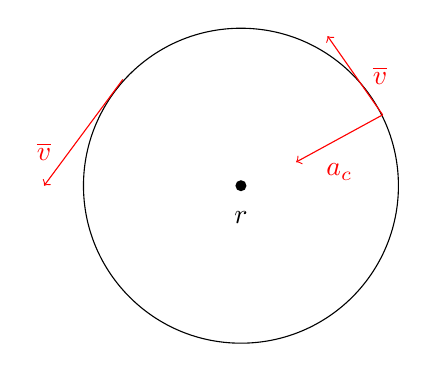
\begin{tikzpicture}
  \fill[black](0,0) circle (2pt) node[below=2mm] {$r$};
  \draw[fill=none](0,0) circle (2.0);
  \draw[red, ->](-1.5,1.35) -- (-2.5,0) node[above=2mm] {$\overline{v}$};
  \draw[red, ->](1.8,0.9) -- (1.1,1.9) node[midway, right=1mm] {$\overline{v}$};
  \draw[red, ->](1.8,0.9) -- (0.7,0.3) node[midway, below=2mm] {$a_c$};
\end{tikzpicture}
\end{figure}

We can define a few variables that relate to this motion. First out is $T$, the \emph{period} in seconds it takes the object to travel along the entire circumference once. Second is the \emph{frequency} $f$, which measures how many times it travels around the circle per second. The two are then inverses, so that $f = 1/T$ and $T = 1/f$.\\
The SI unit for frequency is Hertz; the dimension is then $\text{dim Hertz} = \displaystyle \frac{1}{[T]}$, and $\SI{1}{Hertz} = \SI{1}{s^{-1}}$.

We can consider how fast it moves in a different way, in measuring velocity in \emph{radians per second}, instead of meters per second (or other units of ``regular'' velocity). We call this \emph{angular velocity}, symbol $\omega$. Since there are $2\pi$ radians in a circumference, this implies that

\begin{equation}
\omega = \frac{2 \pi}{T}
\end{equation}

As for the speed $v$ (not the velocity $\vec{v}$ just yet), we can write

\begin{equation}
v = \frac{2 \pi r}{T} = \omega r
\end{equation}


\subsection{Centripetal acceleration}

Note that as the object moves around in a circle, the direction of the velocity vector in constantly changing. This can only happen if there is a nonzero acceleration. This acceleration is called the \emph{centripetal acceleration}, often denoted by $\vec{a_c}$. This acceleration vector always points towards the center of the motion. Because the velocity vector is always tangent to the circle at any given point, the acceleration vector is always perpendicular to the velocity, assuming a constant \emph{speed} around the circle. 

The magnitude of the centripetal acceleration can be stated as

\begin{equation}
|a_c| = \frac{v^2}{r} = \omega^2 r
\end{equation}

\subsubsection{Proportionality of $r$}
Be careful when it comes to the proportionality of $r$. If $T$ is held constant, $v$ is a function of $r$, being equal to

\begin{equation}
v = \frac{2 \pi r}{T}
\end{equation}

and so increasing $r$ will also increase $v$, and thus in the end increase $a_c$:

\begin{equation}
|a_c| = \frac{v^2}{r} = \frac{4 \pi^2 r^2}{r T^2} = \frac{4 \pi^2 r}{T^2}
\end{equation}

Here, it's obvious that increasing $r$ will increase $a_c$, assuming $T$ is held constant. This should come as no surprise, as we are increasing our speed $v$ by moving a longer distance in the same amount of time.

However, let's not fool ourselves into believing that $a_c \propto r$ is always a correct view! Let's now look at the case where we hold the velocity constant (thus changing T) while changing the radius. To get a nice look of how this works, we use the simple equation

\begin{equation}
|a_c| = \frac{v^2}{r}
\end{equation}

Here, holding $v$ constant, it's clear that the centripetal acceleration goes \emph{down} as we increase the radius of the circle we travel in.


\subsection{Planetary orbits}

Let's now have a quick look at the orbits of planets. We will look at them much closer in a few weeks, but until then, let's assume (incorrectly) that orbits are circular. (In reality, they are slightly elliptical.)\\
First out, we have a lecture question:

``The radius of Earth's orbit is $150 \times 10^6$ km. Assuming that the orbit is circular, what is the centripetal acceleration of the Earth?''

They want the answer in $\text{km/yr}^2$, so we shouldn't have to do any ugly conversions.\\
Let's see. The period is one year, by definition (not exactly 365.00 days, but that's another story).

Because $\omega = \frac{2\pi}{T}$ and $T = 1$ year, we find $\omega^2 = 4\pi^2$ radians per year, and $\omega^2 r = (4 \pi^2)(\num{150e6}) = \SI{5.92e9}{km/yr^2}$.

Just to make sure, let's also calculate it using $v^2/r$.

$v$ is found by dividing the circumference of the orbit by the time (1 year), which in then equal in value (but obviously not units) to just the circumference. We then square that, and divide by the radius again; a bit redundant to divide out the radius, but let's go with it for simplicity:

\begin{equation}
v = \frac{2 \pi r}{T} = \frac{2 \pi r}{1 \text{ year}}
\end{equation}

\begin{equation}
a_c = \frac{v^2}{r} = \frac{4 \pi^2 r^2}{r} = 4 \pi^2 r = \SI{5.92e9}{km/yr^2}
\end{equation}

Unsurprisingly, we get the same answer. Still, we have now double-checked, and have also gained a bit of practice doing in two different ways.

Now, let's have a look at the orbits of various planets -- their mean distance to the sun (mean, since the orbits are not truly circular) and periods, and let's compare the centripetal acceleration of various planets. What we find can be seen on this plot below:

\begin{figure}[H]
  \centering
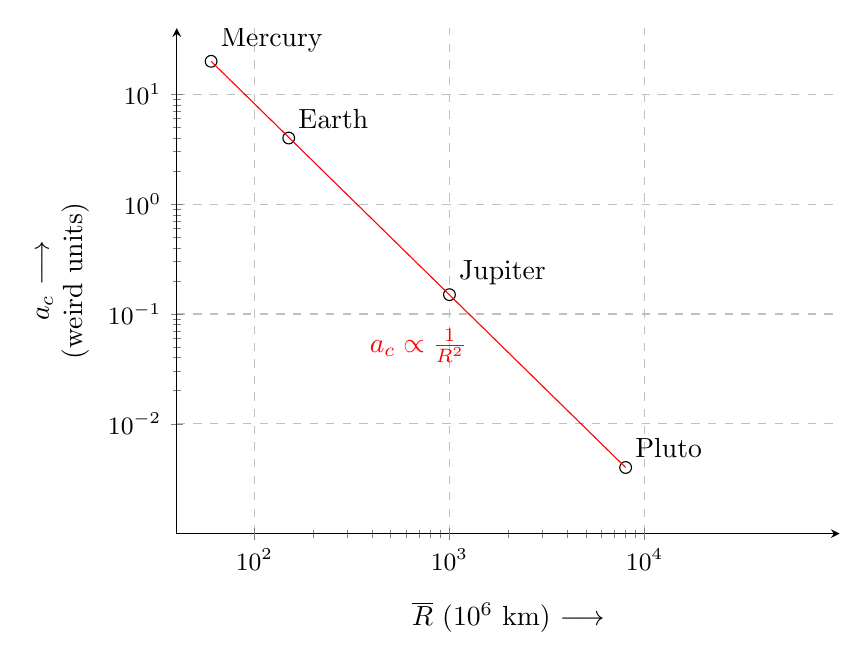
\begin{tikzpicture}
  % Logarithmic plot settings
  \begin{loglogaxis}[
      width=10cm,
      height=8cm,
      xlabel={$\overline{R}$ ($10^6$ km) $\longrightarrow$},
      ylabel style={align=center},
      ylabel={$a_c$ $\longrightarrow$\\(weird units)},
      xmin=4e1, xmax=1e5,
      ymin=1e-3, ymax=4e1,
      xtick={1e2, 1e3, 1e4},
      ytick={1e-2, 1e-1, 1e0, 1e1},
      axis x line=bottom,
      axis y line=left,
      extra x ticks={1e2, 1e3, 1e4},
      extra x tick labels={\phantom{}, \phantom{}, \phantom{}},
      tick label style={font=\small},
      grid=major,
      grid style={dashed, gray!50}
  ]

  % Red line representing ac ∝ 1/R^2
  \addplot[red, thick, domain=1e2:1e4] {1/x^2};

  % Points for planets
  \node[circle, draw=black, fill=white, inner sep=1.5pt] at (axis cs:6e1,2e1) {};
  \node[above right] at (axis cs:6e1,2e1) {Mercury};

  \node[circle, draw=black, fill=white, inner sep=1.5pt] at (axis cs:15e1,4e0) {};
  \node[above right] at (axis cs:15e1,4e0) {Earth};

  \node[circle, draw=black, fill=white, inner sep=1.5pt] at (axis cs:1e3,15e-2) {};
  \node[above right] at (axis cs:1e3,15e-2) {Jupiter};

  \node[circle, draw=black, fill=white, inner sep=1.5pt] at (axis cs:8e3,4e-3) {};
  \node[above right] at (axis cs:8e3,4e-3) {Pluto};

  % Annotation for the red line
  \draw[red] (axis cs:6e1,2e1) -- (axis cs:8e3,4e-3) node[midway, below=7mm] {$a_c \propto \frac{1}{R^2}$};

  \end{loglogaxis}
\end{tikzpicture}
\end{figure}


(It's a bit fun to note that Pluto was still considered a planet when the lecture was recorded! Little has changed in classical mechanics since then, but that one thing certainly has.)

Here, we see the centripetal acceleration on the vertical axis, and the mean distance to the sun on the horizontal. It's clear that the $1/R^2$ fit is rather brilliant! The closer a planet is to the sun, the stronger the centripetal acceleration is, and it falls off following the inverse square law.


\subsection{Centrifuges and more on centripetal acceleration}

Let's now look at the rotation of a glass tube, with a marble inside. The glass tube starts out horizontal, with the marble inside it (see the first picture below):

\begin{figure}[H]
  \centering
\begin{subfigure}[b]{0.4\textwidth}
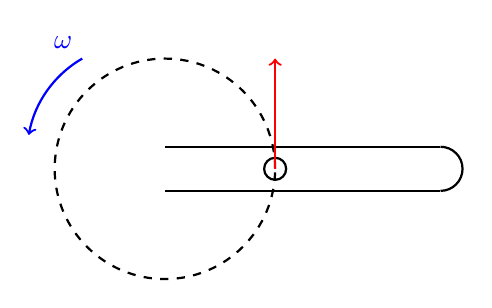
\begin{tikzpicture}[scale=0.7]
  % Draw the dashed circular path
  \draw[dashed, thick] (0,0) circle [radius=2cm];

  \pgfmathsetmacro{\x}{0}
  \pgfmathsetmacro{\r}{0.4}
  \pgfmathsetmacro{\l}{5}

  \draw[thick] (\x,\r) -- (\x+\l,\r);
  \draw[thick] (\x+\l,\r) arc[start angle=90, end angle=-90, radius=\r cm];
  \draw[thick] (\x,-\r) -- (\x+\l,-\r);

  % Draw the small circle at the end of the bar
  \draw[thick] (2,0) circle [radius=0.2cm];

  % Radial arrow (vertical)
  \draw[->, thick, red] (2,0) -- (2,2);

  % Angular velocity arrow
  \draw[->, thick, blue] (-1.5,2) arc[start angle=120, end angle=170, radius=2cm];
  \node[above left, blue] at (-1.5,2) {$\mathbf{\omega}$};

\end{tikzpicture}
\
\end{subfigure}
\begin{subfigure}[b]{0.4\textwidth}
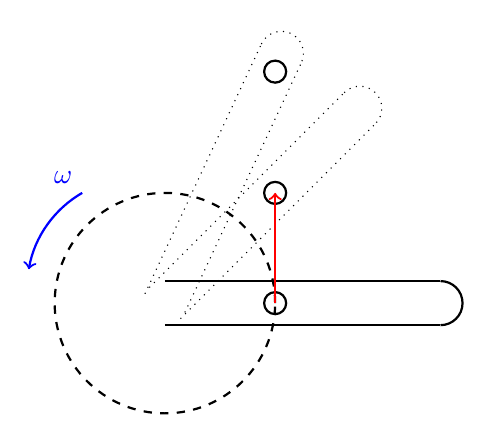
\begin{tikzpicture}[scale=0.7]
  % Draw the dashed circular path
  \draw[dashed, thick] (0,0) circle [radius=2cm];

  \pgfmathsetmacro{\x}{0}
  \pgfmathsetmacro{\r}{0.4}
  \pgfmathsetmacro{\l}{5}

  \draw[thick] (\x,\r) -- (\x+\l,\r);
  \draw[thick] (\x+\l,\r) arc[start angle=90, end angle=-90, radius=\r cm];
  \draw[thick] (\x,-\r) -- (\x+\l,-\r);

  \begin{scope}[rotate around={45:(0,0)}]
  \draw[dotted] (\x,\r) -- (\x+\l,\r);
  \draw[dotted] (\x+\l,\r) arc[start angle=90, end angle=-90, radius=\r cm];
  \draw[dotted] (\x,-\r) -- (\x+\l,-\r);
  \end{scope}

  \begin{scope}[rotate around={65:(0,0)}]
  \draw[dotted] (\x,\r) -- (\x+\l,\r);
  \draw[dotted] (\x+\l,\r) arc[start angle=90, end angle=-90, radius=\r cm];
  \draw[dotted] (\x,-\r) -- (\x+\l,-\r);
  \end{scope}

  % Draw the small circle at the end of the bar
  \draw[thick] (2,0) circle [radius=0.2cm];
  \draw[thick] (2,2) circle [radius=0.2cm];
  \draw[thick] (2,4.2) circle [radius=0.2cm];

  % Radial arrow (vertical)
  \draw[->, thick, red] (2,0) -- (2,2);

  % Angular velocity arrow
  \draw[->, thick, blue] (-1.5,2) arc[start angle=120, end angle=170, radius=2cm];
  \node[above left, blue] at (-1.5,2) {$\mathbf{\omega}$};

\end{tikzpicture}
\end{subfigure}
\end{figure}

Because the glass and the marble are both very smooth, the glass can neither push nor pull on the marble, and so cannot provide any centripetal acceleration. What happens? Well, the glass tube will still rotate, of course -- we assume it's powered by a motor of some kind. The marble, on the other hand, will continue on moving according to its still unchanged velocity vector.

A moment later in time (second picture above), the tube has rotated such that the marble's velocity will take it towards the end of the tube, where we know from experience it will also stay, as long as the tube rotates quickly enough.

\subsection{Artificial gravity through centripetal acceleration}

Let's now look at ``perceived gravity'', or artificial gravity.

\begin{figure}[H]
  \centering
\begin{subfigure}[b]{0.4\textwidth}
  \centering
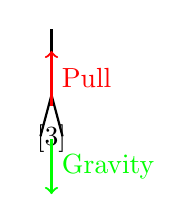
\begin{tikzpicture}[scale=0.7]

  \node at (0, 0) {\Strichmaxerl[3]};
  \draw[thick] (-0.2,0.05) -- (0,0.8);
  \draw[thick] (0.2,0.05) -- (0,0.8);
  \draw[thick] (0,0.8) -- (0,2);
  \draw[thick, red, ->] (0,0.6) -- (0,1.6) node[midway, right] {Pull};
  \draw[thick, green, ->] (0,0) -- (0,-1) node[midway, right] {Gravity};

\end{tikzpicture}
\end{subfigure}
\
\begin{subfigure}[b]{0.4\textwidth}
  \centering
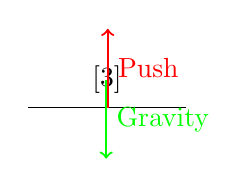
\begin{tikzpicture}[scale=1]

  \node at (0, 0) {\Strichmaxerl[3]};
  \draw (-1,-0.35) -- (1,-0.35);
  \draw[thick, red, ->] (0.01,-0.35) -- (0.01,0.65) node[midway, right] {Push};
  \draw[thick, green, ->] (-0.01,0) -- (-0.01,-1) node[midway, right] {Gravity};

\end{tikzpicture}
\end{subfigure}
\end{figure}
As the illustration shows, we will always experience gravity opposite to any pull or push. The same is true if we somehow hang on to a rope and spin around -- or ride a merry-go-round or something to that effect. We will have a centripetal force inwards, and feel a ``pull'' inwards, but perceive gravity in exactly the opposite direction, as if we were drawn outwards.

Let us now consider a large, circular space station, which experiences almost no gravity (as it is in orbit, essentially in perpetual free fall). It is a big ``wheel'', with a radius of 100 m. We want the centripetal acceleration to be about \SI{10}{m/s^2} for a person standing on the outer wall. How fast should it rotate (what should be the period)?

\begin{figure}[H]
  \centering
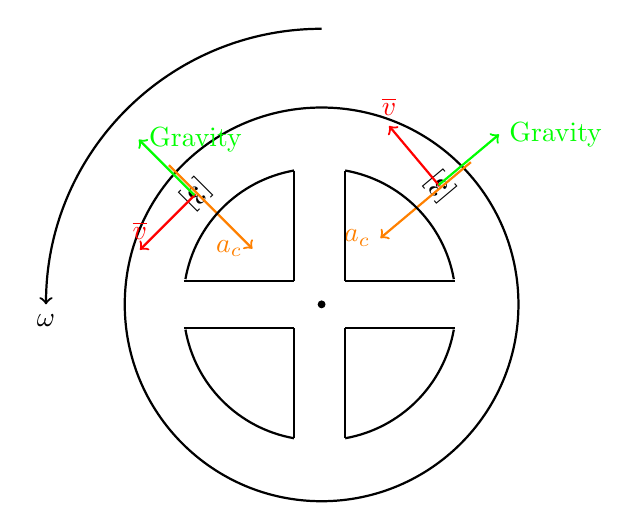
\begin{tikzpicture}[scale=1]

  \draw[thick] (2,0) circle [radius=25mm];
  \fill (2,0) circle [radius=0.5mm];

  \pgfmathsetmacro{\rotate}{130}
  \begin{scope}[xshift=35mm, yshift=15mm]
  \begin{scope}[rotate=\rotate]
    \node at (0, 0) {\rotatebox{\rotate}{\Strichmaxerl[3]}};
    \draw[thick, orange, ->] (-0.02,-0.5) -- (-0.02,1) node[left] {$a_c$};
    \draw[thick, red, ->] (0,0) -- (1,0) node[above] {$\overline{v}$};
    \draw[thick, green, ->] (0.02,0) -- (0.02,-1) node[right] {Gravity};
  \end{scope}
  \end{scope}

  \pgfmathsetmacro{\rotate}{-135}
  \begin{scope}[xshift=4mm, yshift=14mm]
  \begin{scope}[rotate=\rotate]
    \node at (0, 0) {\rotatebox{\rotate}{\Strichmaxerl[3]}};
    \draw[thick, orange, ->] (-0.02,-0.5) -- (-0.02,1) node[left] {$a_c$};
    \draw[thick, red, ->] (0,0) -- (1,0) node[above] {$\overline{v}$};
    \draw[thick, green, ->] (0.02,0) -- (0.02,-1) node[right] {Gravity};
  \end{scope}
  \end{scope}

  \draw[thick, ->] (2,3.5) arc[start angle=90, end angle=180, radius=35mm] node[below] {$\omega$};

  \draw[thick] (1.65,1.7) arc[start angle=100, end angle=170, radius=17mm];
  \draw[thick] (2.30,1.7) arc[start angle=80, end angle=10, radius=17mm];
  \draw[thick] (2.30,-1.7) arc[start angle=-80, end angle=-10, radius=17mm];
  \draw[thick] (1.65,-1.7) arc[start angle=-100, end angle=-170, radius=17mm];

  \draw[thick] (1.65,-1.7) -- (1.65, -0.3);
  \draw[thick] (1.65,1.7) -- (1.65, 0.3);
  \draw[thick] (2.30,1.7) -- (2.30, 0.3);
  \draw[thick] (2.30,-1.7) -- (2.30, -0.3);

  \draw[thick] (0.25,0.3) -- (1.65,0.3);
  \draw[thick] (0.25,-0.3) -- (1.65,-0.3);
  \draw[thick] (2.30,-0.3) -- (3.70,-0.3);
  \draw[thick] (2.30,0.3) -- (3.70,0.3);

\end{tikzpicture}
\end{figure}

We can use $\omega^2 r$ here; it should equal \SI{10}{m/s^2}, so we find

\begin{align}
(\omega^2)(\SI{100}{m}) &= \SI{10}{m/s^2}\\
\omega^2 &= \frac{\SI{10}{m/s^2}}{\SI{100}{m}}\\
\omega^2 &= \SI{0.1}{rad^2/s^2}\\
\omega &= \sqrt{0.1} \text{ rad/s}
\end{align}

And, because $\omega = \frac{2 \pi}{T}$:

\begin{align}
\frac{2 \pi}{T} &= \sqrt{0.1}\\
T &= \frac{2 \pi}{\sqrt{0.1}} \approx \SI{20}{s}
\end{align}

So if we rotated the space station with a period of about/just over 20 seconds, we would perceive it as if we had Earth's gravity.

The gravitational acceleration is zero at the center, but it grows as you come closer to the outer edge. If you were to ``jump'' down the shaft, you would end up crashing into the outer wall at a velocity great enough that you may well be killed!


\section{Lecture 6: Newton's first, second, and third laws}

In this lecture, we will introduce the concept of \emph{force}, an extremely important quantity in physics. Last lecture used forces, but referred to them as ``pushes'' or ``pulls''. We will now start using the correct terminology.

\subsection{Newton's first law}

Newton's first law essentially dates back to Galileo Galilei, in his ``law of inertia''.\\
Newton wrote it as

\begin{quote}
Every body perseveres in its state of rest, or uniform motion in a right line, unless it is compelled to change that state by forces impressed upon it.
\end{quote}

This means that if we perceive ourselves to be at rest unless we experience an unbalanced force such as an acceleration
of a car we are in. We do experience forces we stand still: the gravitational force and the normal force. However,
those cancel each other out.

Newton's first law, however, is not valid in all reference frames. It is only valid in inertial references frames, the definition of which is a reference frame where the motion of a particle not under any forces moves in a straight line at constant speed. In particular, this is not true in a reference frame which is being accelerated in any way.

So the question is: can we find an inertial reference frame? Is the lecture hall an inertial reference frame, for example?\\
In can't be. The Earth spins, causing a centripetal acceleration. That's an acceleration, so the answer is already no. There are many additional reasons, though: the Earth moves around the Sun, again causing centripetal acceleration. The Sun moves around the galaxy's center, the galaxy itself has an orbit, and so on.

The Earth has, as mentioned, a centripetal acceleration. We can estimate it by calculating $\omega^2 R_{earth}$, which turns out to be about \SI{0.034}{m/s^2}, which is of course much, much lower than the acceleration due to gravity. If the Earth spun much, much faster, the centripetal acceleration might start to cancel out gravity noticeably, however.

Let's then calculate the centripetal acceleration due to the orbit around the Sun. The radius of the orbit is about $\SI{150e9}{m}$, and the period is of course one year.

\begin{align}
\omega &= \frac{2 \pi}{T} = \frac{2 \pi}{365 \cdot 24 \cdot 60 \cdot 60} = \SI{1.992e-7}{rad/s}\\
a_c = \omega^2 r &= (\SI{1.992e-7}{rad/s})^2 \times \SI{150e9}{m} = \SI{5.95e-3}{m/s^2}
\end{align}

Because the centripetal accelerations calculated above are so tiny, we can consider the Earth as being very close to an inertial reference frame.

A mathematical statement of Newton's first law might be

\begin{equation}
\sum \vec{F} = 0 \Rightarrow \frac{d\vec{v}}{dt} = 0 \text{ (Newton's first law)} \label{eq:newton1}
\end{equation}

\subsection{Newton's second law}

Say we have a spring (though the law isn't specific to springs), in the absence of gravity. We extend the spring, and attach a mass $m_1$ at the end of the spring.

\begin{figure}[H]
     \centering
\begin{tikzpicture}
     % Draw a spring
     \draw[decorate, decoration={aspect=0.5, segment length=5mm, amplitude=3.5mm, coil}] 
         (0,0) -- (5,0);
     \fill[black] (5,0) circle (3mm) node[above right = 3mm and 2mm] {$m_1$};
     \draw[thick] (0,-1) -- (0,1);
     \draw[thick, red, -{Stealth[scale=1.5]}] (5,0) -- (3,0) node[midway, above = 4mm] {pull};
     \draw[dotted] (2.4, -1) -- (2.4, 1);
 \end{tikzpicture}
\end{figure}

Immediately after we let go of the mass, so that the spring's ``pull'' contracts the spring and pulls the mass with it, we measure the acceleration of the mass to be $a_1$.\\
We then replace the mass with another mass $m_2$, and measure the acceleration, in the same manner, to be $a_2$.

We will then find that $m_1 a_1 = m_2 a_2$. The product $m a$ is the \emph{force} (which we have called a ``push'' or a ``pull'' until now) exerted upon the mass by the spring. The spring's force is independent on the mass, but the acceleration caused on the mass is not; the acceleration is inversely proportional to the mass.

In equation form, Newton's second law -- one of the most important equations in physics -- reads

\begin{equation}
\vec{F} = m \vec{a} \text{ (Newton's second law)} \label{eq:newton2}
\end{equation}

As shown above, force is a vector. The direction of the acceleration caused by a force is always in the same direction as the force.

The SI unit for force is the newton, in honor of Newton himself, of course. Because the product $m a$ is in units of $\displaystyle \text{kg} \cdot \frac{\text{m}}{\text{s}^2}$, 1 newton equals 1 $\displaystyle \text{kg} \cdot \frac{\text{m}}{\text{s}^2}$.

Just as with the first law, we cannot truly prove Newton's second law. Like the first, it is only valid in inertial reference frames, and we cannot provide such a reference frame to conduct our experiments in.

Note that no statement is made regarding speed or velocity, only acceleration. The law holds equally well at 0 m/s, 5 m/s and 5000 m/s. However, once speeds start becoming noteworthy in relation to the speed of light, Newtonian mechanics becomes more and more inaccurate, and we instead need to use Einstein's relativity for accurate results. 

\subsection{Newton's third law}

Let's now have a look at the gravitational force. Using the second law, we see that the force is equal to $m \vec{g}$. Double the mass, double the force, etc.\\
We assume that the lecture hall is an inertial reference frame. Consider an object that is at rest (relative to the lecture hall). We know from the above that there must be a gravitational force on the object, pulling it downwards. However, it is at rest, so there is no acceleration (in our reference frame). Therefore, the net force on it \emph{must} be zero. This is only possible, of course, if there is an equal and opposite force -- or sums of forces that adds up to exactly cancel the gravitational force out.

The above is the result of the third law, which can be stated as

\begin{quote}
If one object exerts a force on another, the other exerts the same force in the opposite direction on the one.
\end{quote}

In other words, if gravity pulls you down into your chair with a force of, say, 700 N, then the chair exerts a force of 700 N back on you. It can be stated more simply as $\text{action} = -\text{reaction}$.\\
We can therefore also write the law as

\begin{equation}
\vec{F_{12}} = -\vec{F_{21}} \text{ (Newton's third law)} \label{eq:newton3}
\end{equation}

where $\vec{F_{ab}}$ means the force exerted \emph{by} object a \emph{on} object b. Note that some physics textbook authors use the reverse notation, which can get confusing.

Unlike the first and second laws, the third laws always holds, including in accelerated reference frames.


\subsection{Examples of Newton's laws in use}

Let's look at a few examples of Newton's law in practice.

\begin{figure}[H]
     \centering
\begin{tikzpicture}

     \draw[thick] (0,0) rectangle (1,1) node[midway] {$1$} node[midway, above=9mm] {$m_1=5$};
     \draw[thick] (1,-0.5) rectangle (3,1.5) node[midway] {$2$} node[midway, above=10mm] {$m_2=15$};

     \draw[thick, red, -{Stealth[scale=1.5]}] (-2,0.5) -- (0,0.5) node[above left=4mm] {$\overline{F}=20$};
 \end{tikzpicture}
\end{figure}



There's a force of 20 newtons towards the right, as shown. Because the total mass is 20 kg, and the force is 20 newton, there will be an acceleration of $\SI{1}{m/s^2}$ via $\displaystyle \vec{a} = \frac{\vec{F}}{m}$ -- Newton's second law. If not else, we know from intuition and daily life that both objects will move towards the right together, with the same acceleration (and thus velocity, since they started together), once they start moving.

The entirety of the force is on object 1. Since they move together, there must be a force between object 1 and object 2 ($\vec{F_{12}}$), towards the right, or object two could not accelerate.

Since we know that the force on object 1 from the left is 20 N, and we also know that $m_1 = \SI{5}{kg}$ and $a_1 = \SI{1}{m/s^2}$ to the right, we can use Newton's second law to find the net force on object 1 to be 5 N towards the right, despite the force on it from the left being 20 N.

How come? Well, the answer lies in object 2. We know that $m_2 = \SI{15}{kg}$ and $a_2 = \SI{1}{m/s^2}$, so the net force on object 2 \emph{must} be 15 N towards the right. The \emph{only} force on object 2 is $\vec{F_{12}}$, so that too must be 15 N towards the right.

What about object 1? Well, Because of $\vec{F_{12}}$ being 15 N to the right, there must be a force $\vec{F_{21}}$ of 15 N towards the left, back on object 1, which ``cancels out'' most of the 20 N, and leaves object 1 with a net 5 N force to the right. In math form:

\begin{equation}
\vec{F_1} = \vec{F} + \vec{F_{21}} = +20\hat{x} + (-15\hat{x}) = +5 \hat{x}
\end{equation}

... defining the increasing direction of $x$ being towards the right.

Now, what about the sum of forces on object 2? Don't we have 15 N towards the right from object 1, and 15 N towards the left back to object 1, for a net zero force? No! The fact that $a \neq 0$ is enough to prove that this cannot be the case.

It's important to note and understand that the two forces $\vec{F_{12}}$ and $\vec{F_{21}}$ act on different bodies. They don't cancel each other out on an individual object. $\vec{F_{21}}$ is a force that object 2 exerts on object 1 -- that fact does \emph{not} in any way negate the force exerted by 1 on 2! If that were the case, object 2 could not accelerate, since its net force would be zero.


\subsection{Tension and another example of Newton's laws in use}

Say we hang a mass $m$ from two strings, suspended at different heights. The leftmost string makes an angle of 45 degrees with the roof above, while the rightmost string makes an angle of 60 degrees. We call the tension in the rightmost string $T_1$, and in the leftmost $T_2$. We consider increasing $x$ to be towards the right, and increasing $y$ to be upwards.

\begin{figure}[H]
     \centering
\begin{tikzpicture}
     \draw (0,2) -- (2,0);
     \draw (2,0) -- (3,2);
     \draw[thick] (-1,2) -- (4,2);
     \draw[thick, red, -{Stealth[scale=1.5]}] (2,0) -- (1.5,0.5) node[below = 4mm] {$T_2$};
     \draw[thick, red, -{Stealth[scale=1.5]}] (2,0) -- (2.5,1) node[below = 4mm] {$T_1$};
     \draw[thick, red, -{Stealth[scale=1.5]}] (2,0) -- (2,-1.5) node[below = 2mm] {$mg$};
     \draw[dotted, -{Stealth[scale=1.5]}] (-1,0) -- (-1,1) node[midway, right = 2mm] {$+y$};
     \draw[-{Stealth[scale=1.5]}] (3,-0.5) -- (4,-0.5) node[below = 2mm] {$+x$};
     \draw[dotted] (0,0) -- (4,0);
 \end{tikzpicture}
\end{figure}


There will be a gravitational force of magnitude $m g$ downwards. Because the object is in equilibrium, sitting still with no acceleration, the \emph{net force} on the object must be zero -- that is clear from Newton's second law.\\
Therefore, we conclude that the two tensions $T_1$ and $T_2$ perfectly balance the gravitational force $m g$, so that the net force on the object is zero.

Force is a vector, so we can decompose this into two one-dimensional problems. We don't need to decompose the gravitational force, of course: it is already only in the $-y$ direction. Let's decompose the tension vectors, though.

Let's start with $T_1$. It makes a 60 degree angle with the horizontal, so by using vector decomposition, we find

\begin{align}
T_{1x} &= T_1 \cos(\ang{60}) = \frac{T_1}{2}\\
T_{1y} &= T_1 \sin(\ang{60}) = \frac{T_1 \sqrt{3}}{2}
\end{align}

As for $T_2$, it makes a 45 degree angle, so the sine and cosine are both one over the square root of two. (It makes sense that the force is equal in both directions, since the angle is exactly in the middle of a 90 degree angle, so to speak.)

\begin{align}
T_{2x} &= T_2 \cos(\ang{45}) = \frac{T_2}{\sqrt{2}}\\
T_{2y} &= T_2 \sin(\ang{45}) = \frac{T_2}{\sqrt{2}}
\end{align}

What then? Well, we know that the net force must be zero, since there is no acceleration. The same can be said for each axis independently, too: $\sum F_x = 0$ and $\sum F_y = 0$. We can set up equations representing this:

\begin{align}
T_{1x} + T_{2x} = 0\\
\frac{T_1}{2} - \frac{T_2}{\sqrt{2}} = 0\\
T_1 = \frac{2 T_2}{\sqrt{2}} = \sqrt{2} \cdot T_2 \label{eq:lec6_t1}
\end{align}

Note that because $T_2$ points towards the negative $x$ direction, the sum of these two forces becomes a subtraction.

As for the $y$ axis:

\begin{align}
T_{1y} + T_{2y} = m g\\
\frac{T_1 \sqrt{3}}{2} + \frac{T_2}{\sqrt{2}} = m g\\
T_2 = \sqrt{2}\left(m g - \frac{T_1 \sqrt{3}}{2}\right)
\end{align}

Alternatively, we could have written $T_{1y} + T_{2y} - m g = 0$ (minus $m g$ since it is in the opposite direction) to show that the sum is zero, rather than saying that they must be equal. This is of course the same thing algebraically.

We now have two equations with two unknowns. Let's substitute the value of $T_1$ into the second equation from \eqref{eq:lec6_t1} and find $T_2$ as a function of only $m$ and constants:

\begin{align}
T_2 = \sqrt{2}\left(m g - \frac{\sqrt{2} T_2 \sqrt{3}}{2}\right)\\
T_2 = \sqrt{2} m g - T_2 \sqrt{3}\\
T_2 + \sqrt{3} T_2 = \sqrt{2} m g\\
T_2 (1 + \sqrt{3}) = \sqrt{2} m g\\
T_2 = \frac{\sqrt{2} m g}{1 + \sqrt{3}}
\end{align}

Since $T_1 = \sqrt{2} T_2$, $T_1$ is simply

\begin{equation}
T_1 = \frac{2 m g}{1 + \sqrt{3}}
\end{equation}

We can finally substitute in some values. The lecture used $m = \SI{4}{kg}$, so let's try that. We find

\begin{align}
T_1 &= \frac{(2)(\SI{4}{kg})(\SI{9.8}{m/s^2})}{1 + \sqrt{3}} \approx \SI{28.7}{N}\\
T_2 &= \frac{T_1}{\sqrt{2}} \approx \SI{20.3}{N}
\end{align}

The professor's answers differ slightly, but match up perfectly if we use $g = \SI{10}{m/s^2}$, so he most likely used that approximation.

As a sanity check, and additional practice, let's just make sure that the forces indeed balance out.

\begin{align}
T_1 \cos(\ang{60}) - T_2 \cos(\ang{45}) &\overset{?}{=} 0\\
14.35 - 14.35 &= 0
\end{align}

... so that indeed works out in the $x$ direction. Let's check $y$:

\begin{align}
T_1 \sin(\ang{60}) + T_2 \sin(\ang{45}) &\overset{?}{=} m g\\
24.85 + 14.35 &= 39.2
\end{align}

It works out perfectly!

%%% Local Variables:
%%% TeX-master: "../../../volumes/Physics/main"
%%% End:


\section{Lecture 7: Weight, perceived gravity, and weightlessness}

This lecture will discuss weight, its relation to mass, and other related topics.

A regular scale, say a bathroom scale, measures weight -- which is a \emph{force}.
The force of the scale is $F_s=mg$, the scale uses the gravitational constant of earth $g$.
Thus, there is only one unknown $m$, which can be derived from $m=\frac{F_s}{g}$.

If we were to use the same scale on the moon, which has a mass of $1/6$ of earth, the 
scale would show that your mass is $1/6$ of what it is since it uses $g$ of earth.

Now, we move the scale and you into an elevator.

\begin{figure}[H]
  \centering
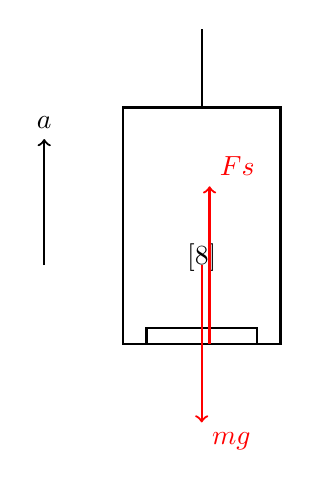
\begin{tikzpicture}
  \pgfmathsetmacro{\ax}{1}
  \pgfmathsetmacro{\ay}{0}
  \pgfmathsetmacro{\bx}{\ax + 2}
  \pgfmathsetmacro{\by}{\ay + 3}
  \pgfmathsetmacro{\cx}{\ax + 1}
  \pgfmathsetmacro{\cy}{\ay+1.1}
  \pgfmathsetmacro{\ddx}{\bx-\ax}
  \pgfmathsetmacro{\dx}{\ax + \ddx/2}

  \draw[thick] (\dx, \by) -- (\dx, \by+1);
  \draw[thick] (\ax, \ay) rectangle (\bx, \by);
  \draw[thick] (\ax+0.3, \ay) rectangle (\bx-0.3, \ay+0.2); % Scale
  \node at (\cx, \cy) {\Strichmaxerl[8]};

  \draw[thick, ->] (0, 1) -- (0, 2.6) node[above] {$a$};
  \draw[thick, red, ->] (\dx+0.1, \ay) -- (\dx+0.1, \ay + 2) node[above right] {$Fs$};
  \draw[thick, red, ->] (\dx, \ay+1) -- (\dx, \ay-1) node[below right] {$mg$};
\end{tikzpicture}
\end{figure}

Again, gravity acts on you with a force $m g$ downwards. The scale pushes back up with force $F_S$. However, now, the elevator is being accelerated upwards. The net force must now be positive (upwards), not zero, since you could not have a nonzero acceleration with zero net force.

We find that $F_S - m g = m a$, so $F_S = m(a + g)$. The reading of the scale has increased, and increases linearly with increasing acceleration upwards. If the elevator accelerates upwards at $2g \approx \SI{20}{m/s^2}$, your weight would be three times as high as usual. Only when $a_y = 0$ is your measured weight as it usually is.

Let's now reverse the situation. We now consider increasing $a$ to be downwards, and the elevator is now accelerating downwards. In other words, $a > 0$.

Again, you have gravity acting downwards with a magnitude $m g$. If that were the only force, you would be in free fall with acceleration $g$, so there must be some upwards acting force. On the other hand, $|m g| > |F_S|$ or there would be no acceleration at all, so while $|F_S|$ is smaller than the force gravity exerts on you, it's still there.

Back to Newton's second law.

\begin{equation}
m g - F_S = m a
\end{equation}

Reading that out loud, it does make a lot of sense: if $F_S = m g$, then $m a$ is zero, and we are not accelerating. If $m g$ is dominant, we are accelerating downwards (since $a > 0$ means downwards acceleration).

Rearranged,

\begin{equation}
F_S = m(g - a)
\end{equation}

The larger the downwards acceleration, the \emph{less} you weigh. I think most of us have experienced this (and the reverse situation) in fast elevators (that accelerate quickly).

Now, imagine we cut the cable of the elevator. What happens? Well, our equation has the answer. The net acceleration $a$ will be equal to the acceleration from gravity $g$, so $F_S = 0$. That is, the scale will show you to have zero weight -- and you will, because you are now in free fall. You are falling downwards, but other than that, you wouldn't notice gravity the same way we do now. The things falling with you wouldn't care about up or down -- a glass filled with water would act the same whether upside down or not.

This is very similar to how things work in the space shuttle and on the International Space Station (ISS). Their orbits around the Earth keep them in constant free fall, only they never hit the surface, as they are going sideways with great velocity (about 7.7 km/s!). We will talk much more about orbits later in the course.

In short, weightlessness is when the forces acting on you are exclusively gravitational. You're not being held up by any floors, ropes, seats, etc, just falling due to gravity pulling on you.

Let's now look at another type of scale:

\begin{figure}[H]
  \centering
\begin{tikzpicture}[scale=1]

  \draw[thick] (0,2) circle (8pt);
  \node at (0,0) {\Strichmaxerl[7]};
  \draw[thick] (0,1.8) -- (0,0.9);
  \draw[thick] (0.4,0.0) -- (0,1.5);
  \draw[thick] (-0.4,0.0) -- (0,1.5);
  \draw[thick] (-0.4,0.0) -- (0,1.5);

  \draw[thick, red, -{Stealth[scale=1.5]}] (0,0.1) -- (0,2) node[midway, right = 2mm] {$T=mg$};
  \draw[thick, red, -{Stealth[scale=1.5]}] (0,-0.1) -- (0,-2) node[midway, right = 2mm] {$mg$};

\end{tikzpicture}
\end{figure}

The scale in this case is a tension meter, inside the string we are hanging from. Because we are hanging still, not accelerating, the tension in the string must equal the force of gravity pulling us down. Therefore, the tension meter reads $m g$, same as it would on a regular scale standing on the floor.\\
Thus, we see that it makes no difference whether we measure the force a scale is pushing us up with, or the force a rope/tension meter \emph{pulls} us up with.

Let's now accelerate this system. We accelerate it upwards, which must mean the tension in the string goes up -- it must be greater in magnitude than $m g$ or we wouldn't accelerate upwards.\\
Just as with the elevator, we find $T - m g = m a$ or $T = m(a + g)$. Same as before, only we use $T$ for tension instead of $F_S$ for force exerted by the scale.\\
If we instead accelerate downwards, we again find the same result as before, as do we if we simply cut the string and go into free fall.

Say we have the following system:

\begin{figure}[H]
  \centering
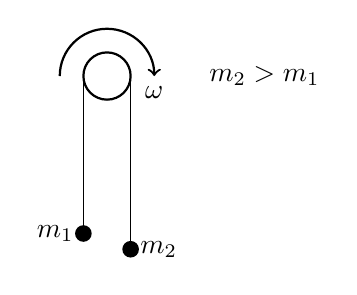
\begin{tikzpicture}[scale=1]

  \draw[thick] (0,2) circle (3mm);
  \fill[thick] (-0.3,0) circle (3pt);
  \fill[thick] (0.3,-0.2) circle (3pt);

  \draw (-0.3,2) -- (-0.3,0) node[left] {$m_1$};
  \draw (0.3,2) -- (0.3,-0.2) node[right] {$m_2$};

  \node at (2,2) {$m_2>m_1$};

  \draw[thick, ->] (-0.6,2) arc[start angle=180, end angle=0, radius=6mm] node[below] {$\omega$};

\end{tikzpicture}
\end{figure}


The string is massless, the pin/pulley is massless, but the two objects hanging an each end are not; the right one at mass $m_2$ has a greater mass than that of $m_1$ to the left.

What happens? Well, we know from intuition and experience that the system will accelerate as shown. $m_2$ will fall down, while $m_1$ will be pulled up.

Because we consider the case where there is no friction, and the string is massless, the tension in the left side must equal the tension on the right side. Only in the case of no friction and a massless string is this true, however.

Why is that, though? It's relatively easy to show. Consider a small piece of the string on the left side. It has gravity pulling the mass $m_1$ down, and a force upwards because of the mass $m_2$ on the other side of the pulley. If the two forces were not equivalent, the massless string would experience an acceleration $a = \frac{F}{0}$ -- that's clearly impossible.	

The same argument can be used for any part (of any length) of the string. The tension must be equal everywhere.\\
Again, this is only true because we consider the string massless, and the pulley frictionless.

Now, we earlier showed that the tension in the string is an indicator of the weight hanging from it. That means that while this acceleration is taking place, $m_1$ and $m_2$ have the same weight! The obviously don't have the same \emph{mass}; that's different, by definition of $m_2 > m_1$. Because weight is mass times acceleration, however, the \emph{weight} of $m_1$ has increased, as it is being accelerated upwards (think about the elevator and the bathroom scale), while the weight of $m_2$ has \emph{decreased}, since it is accelerating downwards (falling, though not in free fall, so it still has a weight larger than zero).

Let's calculate the acceleration and tension for these objects and strings.\\
$m_1$ accelerates upwards. The tension in the string is $T = m_1 g$ while it is in equilibrium, but that cannot be the case now. The force upwards must be greater than $m g$, or it cannot accelerate upwards. Therefore, the tension in the string must be the sum of the downwards force due to gravity, plus the extra ``perceived'' gravity from the upwards acceleration. In total, we have $T = m_1 a + m_1 g = m_1(a + g)$.

For the second object, gravity pulls downwards with force $m_2 g$, while the string tension pulls back up. This object is accelerating downwards, however, so $m_2 g$ must be greater in magnitude than the tension. However, remember that the tension must be the same as in the case of the first mass! It's the same string, and as we showed earlier, we get an impossible situation if the tension differs throughout the string.

To avoid sign confusion, we now denote \emph{downwards} acceleration to be positive. We write the tension out as an equation, and find $T = m_2 (g - a)$.

We now have two equations, so we can set them equal and solve for the acceleration $a$:

\begin{align}
T = m_1(a + g)\\
T = m_2(g - a)\\
m_1 a + m_1 g = m_2 g - m_2 a\\
m_1 a + m_2 a = m_2 g - m_1 g\\
a(m_1 + m_2) = g(m_2 - m_1)\\
a = \frac{g(m_2 - m_1)}{m_1 + m_2}\\
\end{align}

We can then substitute that value into $T - m_1 g = m_1 a$ that we found earlier:

\begin{align}
T - m_1 g = m_1  \frac{g(m_2 - m_1)}{m_1 + m_2}\\
T = \frac{2 g m_1 m_2}{m_1 + m_2}
\end{align}

The algebra isn't shown, but this is indeed the case.\\
These two results make intuitive sense. If we set $m_1 = m_2 = m$, we find $T = m g$ and $a = 0$. All is as it should: the tension on a string with a weight $m$ hanging from it better be $m g$, if it's not accelerating! Likewise, $a$ better be zero, since both masses and weights are equal, so there is no net force on either mass.

If we even consider as $m_2 \to 0$, we find that the tension goes to zero, and the acceleration goes to $g$ (in magnitude). This is because $m_1$ is now in free fall, and since $m_2$ is massless and the string is massless, there is nothing left to cause tension in the string. The acceleration is $-g$ since it is simply in free fall -- nothing is holding it up.

We can also show that if $m_2 > m_1$, then the relationship $m_1 g < T < m_2 g$ will hold for this system. As they are being accelerated, the tension will be equal for both masses. Therefore, $m_1$ must gain weight, and $m_2$ must lose weight. (Keep in mind that $m_1$ accelerates upwards, so it gains weight, like in an elevator, and $m_2$ accelerates downwards, and so it loses weight.)

\subsection{Weightlessness}

We talked a bit about perceived gravity and so on last week. Let's expand on it.

Consider the case where we are swinging an object around a rope of length $R$ in the vertical plane. $R$ is then the radius of the circle the object traces out.\\
Gravity with force $m g$ acts downwards at all times. We spin the object with angular velocity $\omega$.

The string will have a tension $T$, which will change in direction as the thing spins, of course. The magnitude should also change -- if the angular velocity is low, just on the edge of this working out, the tension should be zero at the top. Any slower, and the string will slack off and the object starts falling down.

Let's calculate the tension. First, we know there will be a centripetal acceleration $|a_c| = \omega^2 R$. That must be the case, or the object cannot travel around in a circle like this, period.

At the lowest point of the circle, gravity acts downwards with force $m g$, while the tension upwards is $T$. There's also the centripetal force $m a_c$. We have not really used the term centripetal force yet, but it's a force, so it's found by the centripetal acceleration times the mass in question.

All in all, we find $T - mg = m a_c$, so that $T = m(a_c + g)$. This equation looks almost exactly like the one for acceleration in an elevator, which we found earlier. If $a_c = g$, you tension of the string would be twice the weight of the object.

Now, let's look at the top of the circle instead. As we did earlier, we will now reverse out sign convention so that downwards forces and accelerations are positive.\\
As before, the tension and the force of gravity add up to the centripetal acceleration, so we find $T + m g = m a_c$, so that $T = m(a_c - g)$.

This is just about exactly the same equation as we had for the elevator accelerating downwards, losing weight.\\
If $a_c = g$, the tension will be zero, and the object will be weightless. If $a_c > g$, there will be tension in the string, equal to the object's weight.\\
$a_c$ cannot be smaller than $g$, however. That would give us negative tension, which can't happen. What this implies is that this situation simply would never happen: if $a_c < g$, then the object would never reach the top while tracing out a circle, but would have started falling prior to reaching the top.

The rest of the lecture is mostly demonstrations and related talk, which I didn't find it very useful to take notes for, but it's certainly worth watching, of course.\\
One thing is worth writing down though. The lecture talks about parabolic plane flights -- they start by upwards at a $\approx 45$ degree angle, then follow a parabolic trajectory (free fall) with the engines off, and then re-start the engines and repeat.

This causes the plane to be in free fall for about 30 seconds at a time, during which time any traveler would experience weightlessness -- but \emph{not zero gravity}. There are absolutely similarities between free fall and zero gravity (which you could almost experience far, far from any planets or stars, but certainly not on Earth), but they are not the same.

Zero gravity implies that the Earth's gravity somehow stops acting on the people in the plane, despite the fact that Earth's gravity is almost as strong up there as it is at the surface. Even at the ISS, in orbit at an altitude of about 350 km (which is quite close to the surface for a ``space'' station, all things considered), the gravitational pull is about 90\% of the strength it is near the surface.\\
The astronauts are then weightless for exactly the same reason: they are constantly falling ``towards'' the Earth, only they have such a huge sideways velocity, that they never hit it.

We will talk more about gravity later in the course, including how $g$ is calculated etc.

\section{Lecture 8: Frictional forces}

Let's talk about friction. Thus far, we have ignored friction (and air drag) in all problems we've solved; that will now start to change.

Let's look at a simple case to begin with. We have an object at rest, on a flat surface:

\begin{center}
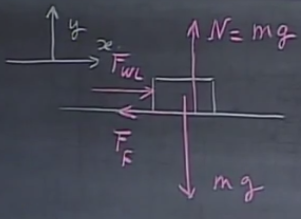
\includegraphics[scale=0.8]{\pIImages/lec8_friction}
\end{center}

There is a gravitational force of magnitude $m g$ pulling the object down, and a \emph{normal force} $N = m g$ (also in magnitude) from the surface on the object, or it could not be at rest; Newton's second law. (Again, however, note that this is NOT a case of Newton's third law; there two forces both act on the object, and so they are not an action-reaction pair.)

We (the professor) exerts a force $F_{WL}$ (WL for Walter Lewin) in the $+x$ direction. Because of friction, the object will not start to move unless the force is great enough. (Without friction, any force, no matter how small, causes an acceleration, even if it's tiny.)

There is a frictional force $F_F$ in the $-x$ direction that exactly cancels out the force we apply. We push harder and harder, and eventually the frictional force reaches its maximum value, at which point we overcome it and the object starts to accelerate.

It is then experimental fact that this maximum, $F_{Fmax}$, is

\begin{equation}
F_{Fmax} = \mu N
\end{equation}

where $\mu$ is a friction coefficient.\\
We can differentiate between the \emph{static} friction coefficient $\mu_s$ and the \emph{kinetic} (or dynamic) friction coefficient $\mu_k$.

$\mu_s N$ is the frictional force we need to overcome to get a resting object to start moving, while $\mu_k N$ is the force we need to overcome to keep accelerating it. (If $\mu_k N = F$, there is zero net force, and so no acceleration. If $\mu_k N > F$, the object will slow down.)\\
We know from experience that it takes more force to get something to move in the first place, so $\mu_s > \mu_k$ -- ``always'', the lecture says, but there does appear to be some strange exceptions to this rule. I'm assuming this course will not cover (or mention) them, however.

We can calculate a friction coefficient by putting an object on an incline, and measure the angle of incline required to get the object to move (due to the gravitational force downwards, of course).

\begin{center}
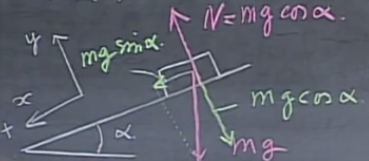
\includegraphics[scale=0.8]{\pIImages/lec8_friction_incline}
\end{center}

Note the choice of coordinate system, which is tilted such that the acceleration (and movement) in the $y$ direction will always be zero, but more importantly such that the $y$ axis is exactly perpendicular to the surface of the incline.\\
The downside to this approach is then that we need to decompose the gravitational force, since it is no longer strictly in one axis.

Because of how the angle $\alpha$ is defined, the strength of the gravitational force in the $y$ direction is $m g \cos \alpha$ (if $\alpha = 0$, $\cos \alpha = 1$ and so it is strictly in the $y$ direction), while that in the $x$ direction is $m g \sin \alpha$. This is a bit opposite to how it usually is ($x$ tends to use the cosine, while $y$ uses the sine), but it should make sense why this is.

There is a normal force $N$ opposing $m g \cos \theta$, which must be equal in magnitude -- there is no acceleration in the $y$ direction, so the net force along that axis must be zero, via Newton's second law.

There is a frictional force $F_F$ in the negative $x$ direction, equal in magnitude to $m g \sin \alpha$ (the gravitational force along the slope), since the object is still not moving. We gradually increase the angle, which increases $F_f$, but of course also the gravitational force in the $x$ direction (downwards along the slope). Sooner or later, the frictional force reaches its maximum, and gravity ``wins''.

How do we then calculate $\mu_s$, the static friction coefficient, in terms of the angle $\alpha_{max}$ (the maximum angle possible before the object starts to slide)?

Well, it should be easy! We know the strength of the force pulling the object: $m g \sin (\alpha_{max})$. We know that $F_F = \mu_s m g \sin (\alpha_{max})$ must exactly equal this force in magnitude to keep it standing still.\\
We also know that $F_F = \mu_s N$, as we mentioned earlier.

Therefore, we set the two equal, and we can solve for $\mu_s$. $N = m g \cos \alpha$, so

\begin{align}
\mu_s m g \cos (\alpha_{max}) = m g \sin(\alpha_{max})\\
\mu_s = \frac{m g \sin(\alpha_{max})}{m g \cos (\alpha_{max})}\\
\mu_s = \frac{\sin(\alpha_{max})}{\cos (\alpha_{max})} = \tan(\alpha_{max})
\end{align}

So finding the static friction coefficient is truly simple: measure the maximum angle possible before the object starts to slide, take the tangent of that angle, and you're done! And, since the incline makes a triangle with the vertical height, horizontal length and the incline itself (the hypotenuse), we can measure this even without knowing angles; we can calculate the angle even if we can only measure distances.

Note that two seemingly important quantities are nowhere to be seen in this result: the mass of the object does not matter, and neither does the amount surface area that is in contact with the incline!\\
This means that two parked cars -- a large truck and a small car,will start to slide at the same angle, if they were tilted together, so to speak. Not only does the mass not matter, but the width of the tires (or the number of tires) also does not matter.

These two facts are then demonstrated qualitatively, by sliding a few objects down a wooden plank. Indeed, adding a few times the mass to a plastic container didn't change the result by much (but by a little -- because the plank is not exactly uniform, the containers may not be identical, etc.). Neither did it make a noticeable difference to slide down two small pieces of wood, one lying down (large contact area) and one standing on the edge (small contact area).

\subsection{Friction on a block with a pulley}

Let's look at a different, but related example. We have the following setup:

\begin{center}
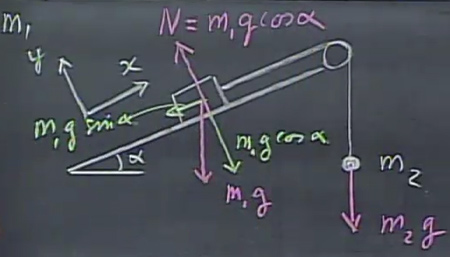
\includegraphics[scale=0.7]{\pIImages/lec8_friction_pulley}
\end{center}

A block of mass $m_1$ is sitting on an incline, with the same gravitational force, decomposed as previously.\\
However, this time, a second mass $m_2$ hangs on a massless and fixed-length string (increasing tension doesn't increase the length of the string), over a pulley (which itself is massless and frictionless).

As before, there is no movement of the  block in the $y$ direction, so we be sure that the normal force $N$ must exactly cancel out the gravitational force of $m_1 g \cos \alpha$ in our rotated $-y$ direction.\\
The string has a tension, since mass $m_2$ is hanging on it. As before, since the string is massless and has a fixed length, the tension must be the same everywhere in the string.

Now... This situation has a tricky part that the previous one didn't: depending on the friction coefficient of the block, and the magnitude of masses $m_1$ and $m_2$, one of three things can happen: the block can accelerate ``downhill'', it can accelerate ``uphill'', or it can simply stand still. We need to consider all of these possibilities when solving this problem. Because of this, we do not know in which direction of the frictional force is; we only know that it always opposes the object's motion, which could be either $+x$ or $-x$.

We do know that the maximum magnitude of the frictional force is

\begin{equation}
F_{Fmax} = \mu_s N = \mu_s m_1 g \cos \alpha
\end{equation}

The tension in the string, $T$, can be drawn as a vector opposing $m_2 g$, in the string above mass $m_2$.

We will now evaluate three different situations. In all cases, the system is at rest for now, but what is about to happen differs: there's the case where it's \emph{just} about to start accelerating towards the left (downhill for the block), the case where it's \emph{just} about to start accelerating in the other direction, and the case where it will remain at rest/in equilibrium.

Because the system is rest, the tension must be of magnitude $m_2 g$, so that it exactly balances the gravitational force on mass $m_2$, and as mentioned previously, that tension is the same in all parts of the string.

\subsubsection{Case 1: About to accelerate uphill}

We will first look at the case where $m_2$ ``wins'', and the block is \emph{just} about to start moving uphill, but is \emph{still at rest}.\\
In this case, the frictional force is at a maximum $F_{Fmax}$, which opposes the direction it's about to move it, so $F_{Fmax}$ acts together with gravity in the $-x$ direction.\\
We can write Newton's second law for the system:

\begin{equation}
T - m_1 g \sin \alpha - F_{Fmax} = 0\text{ (we substitute $T = m_2  g$)}
\end{equation}
\begin{equation}
m_2 g = m_1 g \sin \alpha + F_{Fmax}
\end{equation}

Tension acts ``uphill', while the other two act ``downhill'', and they must sum to zero since $a$ is still zero.

When this equation is true, the block is \emph{just} about to move uphill. Therefore, we can write a criterion for the uphill motion:

\begin{equation}
m_2 g \ge m_1 g \sin \alpha + F_{Fmax}
\end{equation}

If $m_2$ increases in mass by even the tiniest bit, the system will start to accelerate so that $m_2$ starts moving downwards.

\subsubsection{Case 2: About to accelerate downhill}

In this case, the frictional force is in the same direction as the tension, and thus in the opposite direction of gravity. We write Newton's second law again:

\begin{equation}
T + F_{Fmax} = m_1 g \sin \alpha\\
\end{equation}
\begin{equation}
m_2 g = m_1 g \sin \alpha - F_{Fmax}
\end{equation}

If $m_2$ is just a tiny bit \emph{smaller} (or $m_1$ greater, or $F_{Fmax}$ smaller), the system will start moving downhill. Therefore, the criterion for downhill motion is

\begin{equation}
m_2 g \le m_1 g \sin \alpha - F_{Fmax}
\end{equation}

\subsubsection{Case 3: Neither case matches}

In case neither of the two conditions are met, the system will simply sit in equilibrium. The frictional force will be ``adjusted'' so that it causes the net force in the $x$ direction to equal zero.

\subsubsection{Example case}

Let $m_1 = \SI{1}{kg}$, $m_2 = \SI{2}{kg}$, $\mu_s = 0.5$ and $\mu_k = 0.4$, while using $g = \SI{10}{m/s^2}$ for our calculations, just to get an idea. Also, let $\alpha = \ang{30}$.

What will happen in a system with these parameters? Well, we have three possible cases, with equations (or inequalities) we can look at. Since both conditions depend on the same three force terms, let's calculate their values:

\begin{align}
m_2 g &= \SI{20}{N}\\
m_1 g \sin \alpha &= \SI{5}{N}\\
F_{Fmax} = \mu_s m_1 g \cos \alpha &\approx \SI{4.33}{N}
\end{align}

Let's now look at each of the two conditions. For the block to start sliding uphill, substituting in the values, we must have $\SI{20}{N} \ge \SI{5}{N} + \SI{4.33}{N}$. Since that is true, the block will indeed start sliding uphill. Let's just verify that the second case is false, just for the sake of argument. We need $\SI{20}{N} \le \SI{5}{N} - \SI{4.33}{N}$, which is certainly not the case. So indeed, only one case matches, and it says the block will start accelerating uphill.

Let's now attempt to calculate the magnitude of the acceleration, and the string tension. We know that it will start moving uphill, so the frictional force is then downhill, in the $-x$ direction. The magnitude of this force now changes, however: the block is in motion, and so we must now use the kinetic friction coefficient $\mu_k$ instead. Using that, we find

\begin{equation}
F_{Fmax} = \mu_k m_1 g \cos \alpha
\end{equation}

We can again write Newton's second law for this case. The tension is uphill, gravity downhill, and friction downhill. Those forces must equal $m_1 a$, where $a$ is the uphill acceleration. (Since the block is now being accelerated, the net forces no longer sum to zero.)

\begin{equation}
T - m_1 g \sin \alpha - \mu_k m_1 g \cos \alpha = m_1 a
\end{equation}

We need a second equation, however. $T$ is unknown -- because $m_2$ is now being accelerated downwards, it is ``falling'' or ``losing weight'', so $m_2 g > T$ or the object could not accelerate down!\\
Since $m_2$ will never change, and we are still on Earth's surface, $g$ can also not change. The only thing that \emph{can} change is the tension. The tension \emph{must} go down, or $m_2$ simply cannot accelerate downwards!

The second equation can be found by thinking about mass $m_2$. Because the string has a fixed length, the acceleration of this mass \emph{must} be equal to that of the block sliding uphill. Anything else and clearly, the string would need to get either longer or shorter, depending on which acceleration was greater.

Because they are equal in magnitude, then, we can write a second law equation for mass $m_2$, using positive values for the downwards direction (so that this $a$ has the same positive sign as the other $a$ uphill):

\begin{equation}
m_2 g - T = m_2 a
\end{equation}

Solving this system, we get a fairly complex answer, unless we substitute in the numbers early. If we do, we find $a \approx \SI{3.85}{m/s^2}$ and $T \approx {SI}{12.3}{N}$. If we don't, we find, after simplification,

\begin{equation}
a = g\ \frac{m_2 - m_1 (\mu_k \cos \alpha + \sin \alpha)}{m_1 + m_2}
\end{equation}

And for the tension:

\begin{equation}
T = g m_1 m_2 \frac{1 + \mu_k \cos\alpha + \sin \alpha}{m_1 + m_2}
\end{equation}

Two things are important to note from the numerical results we found. One is that the acceleration was a positive number. We had already calculated that the block should move uphill, and since the positive $x$ direction is uphill, a negative acceleration would mean it should move backwards. We already know that is not the case, so the acceleration must be positive in this case.

Second, the tension must be smaller than $m_2 g$, or that mass couldn't possibly be accelerating downwards. If $m_2 g$ doesn't ``win'' over the tension, how could the mass be accelerating downwards?

Let's take a quick look at what would happen in the same system, if $m_2 = \SI{0.4}{kg}$ instead. In that case, $m_2 g = \SI{4}{N}$. Let's look at the conditions again. Is it true that $\SI{4}{N} \ge \SI{5}{N} + \SI{4.33}{N}$? No, certainly not. Is it then true that $\SI{4}{N} \le \SI{5}{N} - \SI{4.33}{N}$? No, that's not it, either.

Since neither condition is met, the system will stay as it is, with $a = 0$. Note that the equations we derived just above, for $a$ and $T$, are not valid in this case and cannot be used. They only hold in the case of accelerations upwards, since that is what we derived them for.

What will happen is that the frictional force will be adjusted so that together with the tension, it holds the object up.


\section{Lecture 10: Hooke's law, simple harmonic oscillator}

Say we have a spring, in its ``relaxed'' state, i.e. in equilibrium. We choose to place $x = 0$ at the spring's end, and then extend the spring a distance $x$.

There will be a restoring force that attempts to pull the spring back to its original length. For many springs, it is approximately true that this restoring force $F$ is proportional to the displacement $x$.\\
For an \emph{ideal spring}, we can write the force as

\begin{equation}
F = -k x
\end{equation}

where $k$ is known as the spring constant, and the minus sign signifies that the force opposes the displacement. (If $x$ is positive to the right, the force will be to the left, and vice versa.)\\
This also holds if the spring is compressed (shortened) instead of stretched.\\
The above relation is known as \emph{Hooke's law}.

We can measure this spring constant in a few different ways. Perhaps the simplest would be to hang a mass from a spring and measure how far it extends due to the pull of gravity. When it is in equilibrium, we know that the upwards force from the spring must equal the downwards force due to gravity. Therefore, we can measure $x$ and $m$, and we know $g$, so we can calculate the spring constant:

\begin{align}
|F| = k x &= m g\\
k &= \frac{m g}{x}
\end{align}

Assuming we work in SI units, the units of the spring constant must then be in newtons per meter.

If we instead change the masses, we will get a plot that is a straight line, assuming Hooke's law holds. We can then find $k$ as the slope of this line:

\begin{figure}[H]
  \centering
\begin{tikzpicture}[scale=1]

  \draw[decorate, decoration={aspect=0.5, segment length=5mm, amplitude=3.5mm, coil}] 
      (0,0) -- (0,5);
  \fill[black] (0,0) circle (2mm);
  \draw[thick] (-1,5) -- (1,5);
  \draw[thick, red, -{Stealth[scale=1.5]}] (0,0) -- (0,1) node[midway, right = 3mm] {$F=mg$};
  \draw[thick, red, -{Stealth[scale=1.5]}] (0,0) -- (0,-1) node[midway, right = 3mm] {$mg$};
  \draw[dotted] (-1,1) -- (1,1);
  \draw[dotted] (-1,0) -- (1,0);
 
  \draw[thick] (2.5,0) -- (8,0) node[below] {$\longrightarrow x$};
  \draw[thick] (3,-0.5) -- (3,4) node[left] {$F$};

  \draw[dashed] (3,0) -- (7,4);
  \draw[thick] (4,1) -- (6.8,1);
  \draw[thick] (6.8,1) -- (6.8,3.8);
  \draw[red, decorate, decoration = {brace, amplitude=3mm}] (6.8,3.8) -- (6.8,1) node[midway, right=3mm] {$\Delta F$} node[midway, right=14mm] {$k =\frac{\Delta F}{\Delta x}$};
  \draw[red, decorate, decoration = {brace, amplitude=3mm}] (6.8,1) -- (4,1) node[midway, below=3mm] {$\Delta x$};
 
\end{tikzpicture}
\caption{}
\end{figure}


This is probably a more reliable test than the single calculation above, since it will show if Hooke's law doesn't hold for the particular spring, instead of silently assuming that it does.

Hooke's law has its limitations, as you might expect. It's possible to stretch a spring so far that it permanently changes its shape, in which case the restoring force will not increase linearly, but grow slower than Hooke's law would predict.

Let's look at a second way of measuring the spring constant of a given spring. Say we have another spring, again with $x = 0$ at the end of spring's relaxed length. We extend the spring further, and attach a mass $m$ to the end of the spring. The mass rests on a frictionless surface.

\begin{figure}[H]
  \centering
\begin{tikzpicture}[scale=1]

  \draw[decorate, decoration={aspect=0.5, segment length=5mm, amplitude=3.5mm, coil}] 
      (0,0) -- (5,0);
  \draw[thick] (5,-0.5) rectangle (6,0.5);
  \draw[thick] (0,-1) -- (0,1);
  \draw[dotted] (3,-1) -- (3,1);
  \draw[-{Stealth[scale=1.5]}] (-1,-0.5) -- (-1,0.5) node[right=1mm] {$y$};
  \draw[-{Stealth[scale=1.5]}] (3,-1) -- (5.5,-1) node[right] {$x$} node[at start, below=1mm] {$x=0$};

  \draw[thick, red, -{Stealth[scale=1.5]}] (5.6,-0.5) -- (5.6,1) node[right=2mm] {$N$};
  \draw[thick, red, -{Stealth[scale=1.5]}] (5.5,0) -- (5.5,-1.5) node[right=2mm] {$mg$};
  \draw[thick, red, -{Stealth[scale=1.5]}] (5.5,0) -- (4,0) node[above=2mm] {$F$};
 
  \node at (1,-2) {$T=2\pi\frac{m}{k}$};
 
\end{tikzpicture}
\caption{}
\end{figure}


When we let the mass go, this system will begin to oscillate. The spring force pulls the mass towards the left until it is relaxed, but when that happens, the mass is already moving towards the left, and has inertia in that direction. The spring will be compressed, and now push on the mass, which eventually comes to a halt, accelerates back towards the right, etc.

Because of the relationship shown, which will be derived shortly, we can either calculate a spring constant from a known mass (while using a stopwatch), or we can measure a mass, if we know the spring constant, even in the absence of gravity! Note that there is no relation to $g$ in the formula. The only place where it appears is in the pull of gravity and the normal force, but since the surface is taken to be frictionless, neither force matters for the oscillation period.

It's interesting to note that the amplitude of the oscillation, i.e. how far it moves horizontally from the center point, does not affect the period at all. If the amplitude is small, it will move slowly back and forth, but if the amplitude is large, it will move at much greater speed, to keep the period constant -- assuming Hooke's Law holds.

\subsection{Simple harmonic oscillators: mathematical derivation}

Let's have a look at the situation we have above. We apply Newton's second law to the system, and find

\begin{equation}
m a = - k x
\end{equation}

Written in alternative notation, and divided through by $m$:

\begin{align}
m \ddot{x} + k x = 0\\
\ddot{x} + \frac{k}{m} x = 0
\end{align}

$\dot{x}$ is used to signify the first time derivative of position (velocity), while $\ddot{x}$ is used for the second time derivative (acceleration).

Prof. Lewin calls this last equation ``arguably the most important in all of physics''. It is the equation that governs simple harmonic oscillators; there are many kinds of such oscillators.

First, it is demonstrated that the solution for $x(t)$ should be some form of sinusoid. Trying to keep this as general as possible, we can write

\begin{equation}
x = A \cos(\omega t + \varphi)
\end{equation}

Here, $A$ is the amplitude (how far it swings, from the center point), $\omega$ is the \emph{angular frequency} (not to be confused with angular velocity), in radians/second, and $\varphi$ is the \emph{phase angle}, in radians.

As we have seen many times before,

\begin{equation}
T = \frac{2 \pi}{\omega}
\end{equation}

since if you increase $t$ by $T$ seconds, the argument to the cosine will have increased by $2 \pi$ radians $= \ang{360}$, and the function repeats.

We can write this in terms of frequency (``regular'' frequency in Hertz, i.e. the number times something happens per second, rather than angular frequency):

\begin{equation}
f = \frac{1}{T} = \frac{\omega}{2 \pi}
\end{equation}

(We can think of the last equations as being in radians per second, divided by $2 \pi$ radians; the ``per second'' is then all that remains.)

Next, we substitute our ``trial answer'' into the equation relating $x$ and $\ddot{x}$. To do that, we must first find $\ddot{x}$, i.e. the second derivative of $x$ with respect to time. Keeping in mind the chain rule, we find

\begin{align}
x        &= A \cos(\omega t + \varphi)\\
\dot{x}  &= A \omega (-\sin(\omega t + \varphi) = -A \omega \sin(\omega t + \varphi)\\
\ddot{x} &= -A \omega^2 \cos(\omega t + \varphi)
\end{align}

Now, because $x = A \cos(\omega t + \varphi)$, we can also write

\begin{align}
\ddot{x} = -\omega^2 x
\end{align}

All in all, our differential equation becomes

\begin{equation}
- \omega^2 x + \frac{k}{m} x = 0
\end{equation}

Because this must always hold for all $x$, it must be the case that

\begin{align}
w^2 = \frac{k}{m}\\
\omega = \sqrt{\frac{k}{m}}
\end{align}

With the equation we already had for $T$, it turns out that

\begin{align}
T = 2 \pi \sqrt{\frac{m}{k}}
\end{align}

... as shown in the figure prior to this derivation.

As we can see, the period is independent on the amplitude, and also independent on the phase angle $\varphi$. More on that now.

When we start this oscillation, we can decide two things: how far we stretch the spring before we let the mass go, and how much (if any) of a push we give it, i.e. initial velocity. The amplitude and phase angle will be decided by these \emph{initial conditions}.

Say we give it a push, so that $\vec{v} = -3\hat{x}$ m/s, while it is at $x = 0$ at $t = 0$. With all these conditions, we can find both the amplitude $A$ and the phase angle $\varphi$. We know the equation must hold true at $x = 0$ at $t = 0$, since that's a given, so we plug that in:

\begin{align}
0 = A \cos(\varphi)
\end{align}

This equation can be true in two cases: $A = 0$, or $\cos(\varphi) = 0$. $A$ cannot be 0, because we know there will be an oscillation with a nonzero amplitude. Therefore,

\begin{align}
\cos(\varphi) = 0\\
\varphi = \frac{\pi}{2}, \frac{3\pi}{2}
\end{align}

Either value of $\varphi$ makes the cosine zero. (There are of course an infinite number of such angles, but we restrict them to $0 < \varphi < 2\pi$.)

Since we have a time-varying position, we can take the time derivative to find the velocity as a function of time, and relate that to the initial condition $v = -3$ m/s.

We calculate the time derivative of the equation (which we did earlier), and substitute in the values, including $t = 0$, and set it equal to $-3$ m/s:

\begin{align}
x = A \cos(\omega t + \varphi)\\
\dot{x} = -A \omega \sin(\omega t + \varphi)
\end{align}

Keep in mind that $\dot{x} = v$.\\
In with the values, and solve:

\begin{align}
-3 = -A \omega \sin(\pi/2)\\
-A \omega = -3\\
A = \frac{3}{\omega}
\end{align}

Say the object has a mass $m = \SI{0.1}{kg}$, and the spring has a spring constant of $k = \SI{10}{N/m}$.

We find $\omega$ as

\begin{equation}
\omega = \sqrt{\frac{k}{m}} = 10 \text{ rad/s}
\end{equation}

So $A = 0.3$ meters, and the full equation that explains this oscillation is

\begin{equation}
x(t) = 0.3 \cos(10 t - \frac{\pi}{2})
\end{equation}

\subsection{Motion of a pendulum}

Next up, we have a look at the equations that govern a pendulum's motion.

\begin{figure}[H]
  \centering
\begin{tikzpicture}[scale=1]

  \draw[dotted] (0,0) arc (240:300:50mm);
  \draw[dotted] (2.5,4.3) -- (2.5,-0.7) node[below] {$x=0$};
  \draw[thick] (2.5,4.3) -- (4.6,-0.2) node[midway, right] {$\ell$};;
  \fill (4.6,-0.2) circle (2mm);
  \draw (2.5,3.3) arc (270:295:10mm) node[midway, below] {$\theta$} ;
  \draw[dotted] (4.6,-0.2) -- (0.4,-0.2);
  
  \draw[-{Stealth[scale=1.5]}] (0,1) -- (0,2) node[right=1mm] {$y$};
  \draw[-{Stealth[scale=1.5]}] (0,1) -- (1,1) node[right=1mm] {$x$};

  \draw[thick, red, -{Stealth[scale=1.5]}] (4.6,-0.2) -- (4,1.1) node[right=2mm] {$T$};
  \draw[thick, red, -{Stealth[scale=1.5]}] (4.6,-0.2) -- (4.6,-1.5) node[right=2mm] {$mg$};

  \draw[thick, orange, -{Stealth[scale=1.5]}] (4.6,-0.2) -- (4,-0.2) node[below=2mm] {$T\sin{\theta}$};
  \draw[thick, orange, -{Stealth[scale=1.5]}] (4.6,-0.2) -- (4.6,1.1) node[right=2mm] {$T\cos{\theta}$};
 
  \draw[dotted, thick, orange] (4.6,1.1) -- (4,1.1);
  \draw[dotted, thick, orange] (4,-0.2) -- (4,1.1);
  %\node at (1,-2) {$T=2\pi\frac{m}{k}$};
 
\end{tikzpicture}
\caption{}\label{fig:lec10-oscillation}
\end{figure}



We have a mass $m$ attached to a string of length $\ell$, which is swinging back and forth. We choose a coordinate system with its origin at the pendulum's center, decompose the forces, and write down Newton's second law for the system.

Gravity is pulling downwards on the mass, while there is a tension in the string pulling upwards (but not straight upwards, of course). We decompose this tension, and write down the equation for the $x$ direction:

\begin{equation}
m a_x = m\ddot{x} = - T(\theta) \sin \theta = -T(\theta) \frac{x}{\ell}
\end{equation}

$a$ is towards the right (since that is the positive direction of the coordinate system), but the horizontal component of the tension is towards the left at this moment. The second equality holds for trigonometric reasons.

For the $y$ direction, we find

\begin{equation}
m \ddot{y} = T(\theta) \cos \theta - m g
\end{equation}

We then have two coupled differential equations to solve, which is above this course's level... but we can simplify things a bit.\\
We start out by making some approximations. First out is the small angle approximation, which is usually used to imply that $\sin \theta \approx \theta$ and $\cos \theta \approx 1$ if $\theta \ll 1$ radian (it works quite well up to 0.2 rad $\approx \ang{11.5}$ or so, at least, where $\cos(0.2) \approx 0.98$ and $\sin(0.2) \approx 0.1987$).

There is a second important approximation we can make if we assume the angle will always be small. Have a look at the diagram above (fig~\ref{fig:lec10-oscillation}), and note how the $x$ amplitude is much greater than the $y$ amplitude. For a 5 degree swing, the $x$ motion is about 25 times as large as the $y$ motion, and it is still 11 times as large at 10 degrees.\\
We can therefore approximate the acceleration in the $y$ direction to be zero, so we find

\begin{align}
0 = T(\theta) - m g\\
T = m g
\end{align}

The cosine disappears, since we approximated it to be one, and the left-hand side disappears since $a = \ddot{x} \approx 0$.

We substitute this into our differential equation for $x$, and find

\begin{align}
m\ddot{x} = -m g \frac{x}{\ell}\\
m\ddot{x} + m g \frac{x}{\ell} = 0\\
\ddot{x} + \frac{g}{\ell} x = 0
\end{align}

Compare this to the spring-mass system, which obeyed $\displaystyle \ddot{x} + \frac{k}{m} x = 0$ -- this is another simple harmonic oscillator!

Since the only difference between the differential equations is, practically, two variable names, the solution is of course the same. We find these equations for this system:

\begin{align}
x = A \cos(\omega t + \varphi)\\
\omega = \sqrt{\frac{g}{\ell}}\\
T = \frac{2 \pi}{\omega} = 2 \pi \sqrt{\frac{\ell}{g}}
\end{align}

Keep in mind that these results are limited to the case where the angles are small, and the string can be considered massless in comparison to the mass at the end of the string.

Now, let's compare the results we found for the spring/mass system and the pendulum on a string.\\
For the oscillating spring, the period depends on the spring constant and the mass $m$. This can be explained simply, as follows: when you extend a spring, there is a restoring force, proportional to the distance you extended it. However, the force is not in any way dependent on the mass of the object you attach to the spring; therefore, the acceleration is inversely proportional to the mass, via Newton's second law:

\begin{align}
|a| = \frac{|F_{spring}|}{m} = \frac{k |x|}{m}
\end{align}

If the acceleration is very low, clearly the period must increase.

As for the pendulum, the period is independent on the mass. Why?\\
Again, this can be shown quite easily. If $m$ doubles, $m g$ doubles, and so the tension $T = m g$ must also double (since the $y$ acceleration is the same -- approximately zero). The restoring force $T \sin \theta$ is proportional to $T$, so that doubles as well. If the mass doubles and the force doubles, the acceleration stays exactly the same, and so the period is not affected.

Next, $k$ and $g$. If $k$ is high, the period is short, which makes sense: the acceleration is proportional to $\sqrt{k}$, so for very large $k$ (meaning a very stiff/strong spring -- remember that it's in newtons per meter of displacement) the acceleration is high, and the period low.\\
As for the pendulum, it is \emph{inversely} proportional to $\sqrt{g}$, so if $g$ is low, the period is very large, and it goes to infinity as $g \to 0$. A pendulum could not work in weightlessness, where the perceived gravity is zero, since it relies on gravity to swing. (This too is easy to see: the restoring force is proportional to $g$, so with $g \approx 0$, there shouldn't be any restoring force, nor any string tension.)


\section{Lecture 11: Work, energy and universal gravitation}

\emph{Work} is a measure of the amount of energy a force uses when moving an object. In simple applications, it can be defined as $W = F d$, where $F$ is the magnitude of the force, and $d$ is the distance the object moves.

A more useful definition, still in one dimension, is an integral, which then can take care of non-constant forces as well:

\begin{equation}
W_{AB} = \int_A^B F\ \mathop{dx}
\end{equation}

... where $A$ and $B$ are the $x$ coordinates where the object starts out, and ends up, respectively.

Work is a scalar quantity, and can be negative, zero or positive.\\
It is positive if the force and the displacement are in the \emph{same} direction, and negative if they are in the \emph{opposite} direction. It can be zero, e.g. if there is no displacement.

The SI unit of work is the joule, J, which from the definition clearly is the same as a force of 1 newton times a displacement of 1 meter. We rarely if ever write Nm for work; though Nm and J are mathematically equivalent, Nm is used for torque (which will be introduced later in the course).

Since $\displaystyle F = m a = m \frac{dv}{dt}$, and distance $dx = v dt$, we can rewrite this integral in terms of velocity:

\begin{equation}
W_{AB} = \int_A^B m \frac{dv}{dt} v \mathop{dt} = \int_{v_A}^{v_B} m\ v \mathop{dv} = \Big[ \frac{1}{2} m v^2 \Big]_{v_A}^{v_B} = \frac{1}{2} m \left(v_B^2 - v_A^2\right)
\end{equation}

Here, we have also found the formula for kinetic energy, often notated as $K_E$, $K_e$ or just $K$:

\begin{equation}
K_E = \frac{1}{2} m v^2
\end{equation}

If an object of mass $m$ is moving at velocity $v$, the above formula can calculate its kinetic energy, i.e. how much energy is required to accelerate it to that velocity.

In other words, using the above two relations, we can see that

\begin{equation}
W_{AB} = \Delta K_E = K_{EB} - K_{EA}
\end{equation}

This is known as the \emph{work-energy theorem}. The difference in kinetic energy of an object is equal to the amount of work done on it by the net forces acting on it.\\
If the kinetic energy has increased when moving from point A to point B, the work is positive; if the kinetic energy has decreased, the work is negative, and if the kinetic energy is unchanged, the net work is zero.\\
Note that it's positive for multiple forces to work against each other, such that one provides positive work, a different force provides negative work, etc. such that the \emph{net} work, and thus the change in kinetic energy, can be either positive, negative or zero, depending on the strengths and angles of the forces.

Let's try an applied example. Say an object is moving upwards, while gravity acts on it downwards as you'd expect.\\
We choose the positive $y$ axis to be upwards, so gravity is $-mg\hat{y}$. The object has a velocity $v_A$ where it starts out at point A, and moves upwards to point B while losing speed due to gravity.

We now want to calculate the distance $h$ between points A and B, assuming that the object comes to (temporary) rest at point B.\\
We apply the work-energy theorem, with $\displaystyle K_{EA} = \frac{1}{2} m v_A^2$ and $K_{EB} = 0$.\\
The gravitational force is constant with a magnitude of $m g$, so the work gravity does is $m g h$. The direction of the force is downward, and the motion is upwards, so the work is negative.\\
We set the two equal and solve for $h$:

\begin{align}
- m g h = 0 - \frac{1}{2} m v_A^2\\
g h = \frac{1}{2} v_A^2\\
h = \frac{v_A^2}{2 g}
\end{align}

We have seen this result before, but we found it in a quite different way last time.

As a second example, say we lift an object against gravity, a height $h$ above where it started out. It starts with 0 speed, and also ends up with 0 speed. Via the work-energy theorem, the net work must be zero, since the object's kinetic energy did not change.\\
Gravity still does its work of $|F h| = |m g h|$, only that it's negative here: the force direction is down, and the motion is up. Since gravity does work $- m g h$ on the object, we, who lift it, must then provide positive work $m g h$ in order to make the net work zero.

If we instead reverse the situation, and lower the object closer to the ground, the opposite thing happens. Gravity does positive work $m g h$, while we provide negative work $- m g h$ when lowering the object, and again the net work must be zero, if the object both starts out and ends up with no kinetic energy.

It's important to realize that work, as used in physics, is far from the same as we might think intuitively.\\
If we lower a very heavy object from a height down to the ground, we will have provided negative work, $- m g h$, but we for sure have still \emph{spent} energy burned in our muscles to provide it. We didn't get some sort of added energy reserve from doing so, even though the work is negative.\\
Likewise, we can get tired from holding an object perfectly still (try holding something heavy at arm's length for an extended period of time!), despite the fact that $F d = 0$ and no work has been done.

\subsection{Taking the step to three dimensions}

We can extend what we have above to three dimensions. Say we apply a force $\vec{F}$ over a path. For each tiny point of this path, we can find a vector $\vec{dr}$, which represents a infinitesimal displacement along the line; so small that we can approximate it as a straight line, rather than some form of curve.

\begin{figure}[H]
  \centering
\begin{tikzpicture}[scale=1]

  \begin{axis}[view={-30}{30},no markers,hide axis,zmax=10,
    z post scale=0.5,
    x post scale=1,
    enlargelimits=false,
    ymax=5,ymin=-5,
    xmax=5,xmin=-5]
    \addplot3+[domain=-0:30,samples=200,samples y=0,ultra thick](x-5,{1.8*sin(deg(2*x))},1*x);
  \end{axis}

  \fill (1.29,0.75) circle (0.8mm) node[right] {$A$};
  \fill (5.2,3.55) circle (0.8mm) node[right] {$B$};

  \draw[thick, orange, -{Stealth[scale=1.5]}] (2.7,1.1) -- (1.3,2.4) node[above] {$\overline{F}$};
  \draw[thick, orange, |-|] (2.6,1.0) -- (2.84,1.24) node[below=2mm] {$d\overline{r}$};
  \draw[thick, orange, -{Stealth[scale=1.5]}] (3.3,2.0) -- (5.0,2.8) node[above] {$\overline{F}$};
  \draw[thick, orange, |-|] (3.1,2.0) -- (3.4,1.9) node[below=1mm] {$d\overline{r}$};

\end{tikzpicture}
\end{figure}


The net work done by the force over the entire path is

\begin{equation}
W_{AB} = \int_A^B = \vec{F} \cdot \vec{dr}
\end{equation}

A dot product integral may look scary, but they're not too bad.\\
By the way, the above is a \emph{line integral} (or \emph{path integral}, or \emph{contour integral}): it evaluates an integral along a path.

We can decompose this integral into three one-dimensional integral -- surprise! -- to make it easier to solve. In general terms, we can write the force vector and the displacement vector as sums of components:

\begin{align}
\vec{F}  &= F_x \hat{x} + F_y \vec{y} + F_z \hat{z}\\
\vec{dr} &= dx \hat{x} + dy \hat{y} + dz \hat{z}
\end{align}

With this in mind, we can find $dW$, a small amount of work done by the force over a small distance $dr$, using the definition of the dot product:

\begin{equation}
dW = \vec{F} \cdot \vec{dr} = F_x \mathop{dx} + F_y \mathop{dy} + F_z \mathop{dz}
\end{equation}

Integrate both sides, and we find

\begin{align}
W_{AB} = \int_A^B \vec{F} \cdot \vec{dr} &= \int_A^B \left(F_x \mathop{dx} + F_y \mathop{dy} + F_z \mathop{dz}\right)\\
                                    &= \int_A^B F_x \mathop{dx} + \int_A^B F_y \mathop{dy} + \int_A^B F_z \mathop{dz}
\end{align}

We now have three one-dimensional problems to solve, instead. Not only that, but we've already solved this integral in one dimension. We just need to add it up for the three dimensions:

\begin{equation}
W_AB = \frac{1}{2} m \left( v_{Bx}^2 - v_{Ax}^2 \right) + \frac{1}{2} m \left( v_{By}^2 - v_{Ay}^2 \right) + \frac{1}{2} m \left( v_{Bz}^2 - v_{Az}^2 \right)
\end{equation}

Not pretty... but that's probably the last time we'll see it written like that. Here it is again, re-arranged, but exactly equal to the above:

\begin{align}
W_AB &= \frac{1}{2} m \left( v_{Bx}^2 + v_{By}^2 + v_{Bz}^2 \right) - \frac{1}{2}m  \left( v_{Ax}^2 + v_{Ay}^2 + v_{Az}^2 \right)\\
     &= \frac{1}{2} m \left( v_B^2 - v_A^2 \right)
\end{align}

... and so we find exactly the same result as we did in one dimension.

Let's as an example calculate the work done by gravity while moving an object around in 3D space.

\begin{figure}[H]
  \centering
\begin{tikzpicture}[scale=1]

  % 3D coordinate axes
  \draw (0,0,0) -- (4,0,0) node[right] {\textbf{x}};
  \draw (0,0,0) -- (0,3,0) node[above] {\textbf{y}};
  \draw (0,0,0) -- (0,0,3) node[left] {\textbf{z}};
 
  % Points A and B
  \filldraw[black] (1,1,1) circle (2pt) node[right] {\textbf{A}};
  \filldraw[black] (3,2.5,2.5) circle (2pt) node[right] {\textbf{B}};
 
  % Wavy 3D path from A to B
  \draw[thick, smooth] 
  (1,1,1) 
  to[out=-30, in=-180] (0.7,0.2,0.6) 
  to[out=10, in=220] (0.8,1.6,1.5) 
  to[out=40, in=160] (2.3,1.2,1.8) 
  to[out=-20, in=200] (2.3,2.2,2.1) 
  to[out=-30, in=-90] (3,2.5,2.5);
 
  % Dashed projection lines to XY plane
  %\draw[dashed] (1,1,1) -- (1,1,0);
  %\draw[dashed] (2,2,2) -- (2,2,0);
  \draw[dotted] (3,2.5,2.5) -- (3,0,2.5);
  \draw[dotted] (3,0,2.5) -- (3,0,0);
  \draw[dotted] (1,1,1) -- (1,0,1);
  \draw[dotted] (1,0,1) -- (1,0,0);
 
  % Gravity force vector
  \draw[thick, orange, -{Stealth[scale=1.5]}] (2.3,1.2,1.8) -- (2.3,0,1.8) node[right=2mm] {$-mg\hat{y}$};

\end{tikzpicture}
\end{figure}

We move from a point $A$ to a point $B$, where $y_B - y_A = h > 0$, in other words, point B is higher up than point A.

The force due to gravity is $- m g \hat{y}$, so the integral would be

\begin{equation}
W_{gravity} = \int_A^B \vec{F} \cdot \vec{dr} = \int_A^B (- m g) \mathop{dy} = - m g \int_A^B \mathop{dy} = -m g(y_B - y_A) = -m g h
\end{equation}

The $x$ and $z$ terms disappear, since $F_x = 0$ and $F_z = 0$ -- gravity only acts along one axis, with the way we've defined our coordinate system.

We find that the work done by gravity is negative, as it should be -- the force vector is down, but the object moved higher up. The net work of the force(s) that moved it upwards, in the $y$ direction, is then $+ m g h$.\\
(We can't say anything about the work along the $x$ and $z$ axes without more information, of course.)

Another thing is interesting about this result: it is independent of the path between points A and B. The only thing that matters, as far as gravity is concerned, is the difference in height. If you move an object up 10 meters and back down 9, the work done by gravity is exactly the same as if you'd just moved it up the one meter. The same goes for all and any movement in the x-z plane, which doesn't affect the work done by gravity whatsoever.

Any force that has the property that the work done is the same for any given pair of start/end points, regardless of the path moved in between them, is called a \emph{conservative force}. As we have just shown, gravity is conservative. If a particle starts at one point, moves around in any path whatsoever, and comes back to that exact point, the work done by gravity is always zero.

\subsection{Conservation of mechanical energy}

We can apply the work-energy theorem to the equation above:

\begin{align}
-m g(y_B - y_A)& = K_{EB} - K_{EA}\\
-m g\ y_B - m g\ y_A &= K_{EB} - K_{EA}\\
K_{EA} + m g\ y_A &= K_{EB} + m g\ y_B
\end{align}

This is a very important result. The quantity $m g y$ is what we call \emph{gravitational potential energy}, often $P_E$ or $U$. What the above result says, then, is that the sum of the kinetic and potential energies at point A must equal the sum of the kinetic and potential energies at point B.

\begin{equation}
K_{EA} + U_A = K_{EB} + U_B
\end{equation}

This is known as the \emph{conservation of mechanical energy}, where the mechanical energy of an object is the sum of its kinetic energy and its potential energy. One can be converted into the other, but \emph{as long as the forces involved are conservative}, the sum of the two must stay equal. This condition is an important one! Friction, for example, is \emph{not} a conservative force, and this relationship will no longer hold if frictional forces are involved.\\
Spring forces \emph{are} conservative, however.

The fact that frictional forces are not conservative should be fairly intuitive. The further we move something against friction, the more total work must be done to overcome the friction. You could move something back and forth on a table and the work done by the friction (and you, in moving it) would just increase and increase in magnitude.\\
If you did the same against gravity, moving something up, then back down, etc., the work done (by gravity, or by you) would \emph{not} simply increase without bound.

With the definition of $K_E = \frac{1}{2} m v^2$, it's clear that kinetic energy is zero when the velocity $v$ of an object is zero.\\
What about potential energy? That is zero where $y = 0$, but where is that? It is up to us to decide where to place that point. We are free to choose it, as long as $g$ is the same at both point $A$ and point $B$ (or simply that $g$ is close enough, so that we can neglect the difference).

\subsubsection{Example problem}

\begin{figure}[H]
  \centering
\begin{tikzpicture}[scale=1]

  \draw (0,0) arc (225:315:50mm);
  \draw[thick] (3.5,-0.65) circle (8mm);

  \draw[thick, -{Stealth[scale=1.5]}] (0,-1.45) -- (0,-0.4) node[midway, left] {$y$};
  \draw[dotted] (0,-1.5) -- (8,-1.5) node[above] {$u=0,y=0$};

  \draw[thick, red, -{Stealth[scale=1.5]}] (3.5,-1.45) -- (5,-1.45) node[right=2mm] {$v_C$};
  \fill (3.5,-1.45) circle (0.5mm) node[below] {$C$};

  \draw[thick, red, -{Stealth[scale=1.5]}] (3.5,0.15) -- (2.5,0.15) node[above] {$v_D$};
  \fill (3.5,0.15) circle (0.5mm) node[above] {$D$};

  \draw[thick, red, -{Stealth[scale=1.5]}] (1.5,-1.03) -- (2.3,-1.4);
  \fill (1.5,-1.03) circle (0.5mm) node[above] {$B$};

  \fill (0,0) circle (0.5mm) node[left] {$A$} node[right=2mm] {$v_A=0$};

  \draw[decorate, decoration = {brace, amplitude=1mm}] (-0.5,-1.45) -- (-0.5,0) node[midway, left] {$h$};

  \draw (3.5,-0.725) -- (2.8,-1.0) node[midway, above] {$R$};
  \fill (3.5,-0.725) circle (0.25mm);

  %\draw[thick] (2.5,4.3) -- (4.6,-0.2) node[midway, right] {$\ell$};;
  %\fill (4.6,-0.2) circle (2mm);
  %\draw (2.5,3.3) arc (270:295:10mm) node[midway, below] {$\theta$} ;
  %\draw[dotted] (4.6,-0.2) -- (0.4,-0.2);
  
  %\draw[-{Stealth[scale=1.5]}] (0,1) -- (0,2) node[right=1mm] {$y$};
  %\draw[-{Stealth[scale=1.5]}] (0,1) -- (1,1) node[right=1mm] {$x$};

  %\draw[thick, red, -{Stealth[scale=1.5]}] (4.6,-0.2) -- (4,1.1) node[right=2mm] {$T$};
  %\draw[thick, red, -{Stealth[scale=1.5]}] (4.6,-0.2) -- (4.6,-1.5) node[right=2mm] {$mg$};

  %\draw[thick, orange, -{Stealth[scale=1.5]}] (4.6,-0.2) -- (4,-0.2) node[below=2mm] {$T\sin{\theta}$};
  %\draw[thick, orange, -{Stealth[scale=1.5]}] (4.6,-0.2) -- (4.6,1.1) node[right=2mm] {$T\cos{\theta}$};
 
  %\draw[dotted, thick, orange] (4.6,1.1) -- (4,1.1);
  %\draw[dotted, thick, orange] (4,-0.2) -- (4,1.1);
  %%\node at (1,-2) {$T=2\pi\frac{m}{k}$};
 
\end{tikzpicture}
\caption{}
\end{figure}



We place an object on this ``roller coaster'', at point A, which is $h$ above the line where we choose $y = 0$ and $U = 0$. It gains speed, by converting gravitational potential energy to kinetic energy, until it reaches point C, where the velocity (and the kinetic energy) is at a maximum, while the potential energy is zero, by our definition.

At that point, it reaches the loop. The question is: from what height $h$ must we let it go along the track, so that it manages to move around the loop without falling out before reaching the top?

We can apply the conservation of mechanical energy to this problem, assuming friction is negligible:

\begin{equation}
U_A + K_{EA} = U_B + K_{EB} = U_C + K_{EC} = U_D + K_{ED}
\end{equation}

We let it go from rest at point A, so $K_{EA} = 0$. Our definition of potential energy as $U = m g h$, where $h$ is the height above the plane where $U = 0$.\\
The vertical distance is must travel ``upward'' in going around the circle is twice the radius, so $2R$.

If we equate the total mechanical energy at A, $U_A = m g h$, with the total mechanical energy at any given point, we can find

\begin{align}
m g h &= m g y + \frac{1}{2} m v^2\\
v^2   &= 2g (h - y)
\end{align}

This equation should hold for any point, again assuming we can neglect friction and other forces. At point D, at the top of the loop, the constraint that $a_c > g$ must hold, or we know that it will fall out of the loop, instead of being pushed against it by the centripetal force.

Since centripetal acceleration is given by $\displaystyle a_c = \frac{v^2}{r}$, and we know $v^2$, we can write an inequality for this being larger than $g$, and then solve for $h$, to find the answer to our question about the minimum height we must release the object from.\\
$y = 2 R$ at this point, so

\begin{align}
\frac{2g (h - 2R)}{R} &\ge g\\
2 h - 4R &\ge R\\
2 h &\ge 5R\\
h &\ge \frac{5}{2} R
\end{align}

So if we find a point along the roller coaster where this condition is met, and perhaps add a small amount due to friction, the ball will ``make the loop'', so to speak. Without friction, air resistance etc., it would come up to the exact same height as it started rolling down from.

\subsection{Newton's law of universal gravitation}

Say we have two masses, often named $m$ and $M$ (where it's often the case that $M$ e.g. a planet, and $m$ is smaller; this is of course no requirement, however). The two point masses\footnote{This also works for masses of nonzero size in some cases, more on that at a later time.} are separated by a distance $r$. The force that $m$ experiences because of $M$ is then

\begin{equation}
F = \frac{G M m}{r^2}
\end{equation}

in the direction of $M$ (gravity is always an attractive force), where $G$ is the gravitational constant, not to be confused with $\displaystyle g \approx \frac{G M_{Earth}}{R_{Earth}^2}$ (approximately because Earth's mass is not all at the center; Earth is not a perfect sphere, etc.).\\
$G$ has a value of about $6.67 \cdot 10^{-11}$, with units that need to cancel out with the others, i.e.

\begin{align}
\text{[N]} = \frac{\text{[G]} \text{[kg]}^2}{\text{[meter]}^2}\\
\frac{\text{[N]} \text{[meter]}^2}{\text{[kg]}^2} = \text{[G]}
\end{align}

So in more terse notation, the units of $G$ are $\text{N} \cdot \text{m}^2 \text{kg}^{-2}$.

Because of $F = ma$, so $\displaystyle a = \frac{F}{m}$, we can find the gravitational acceleration due to a mass $M$ to be the force, above, divided by the mass $m$, as already shown in the aside about $g$.

As the formula shows, as the distance from the source of the gravity doubles, the magnitude of the force (or the acceleration) is reduced by a factor of 4.

\subsection{Gravitational potential energy}

Let's now talk about gravitational potential in the general case. Previously, we've only used it where we are near the surface of the Earth, and $g$ has a value that can be considered constant. This is of course not true in general, but there is a definition we can use that is valid everywhere in the universe.

If it is to be valid everywhere, where do we place the zero? There are only two plausible choices, and one (at $r = 0$) turns out to not make much sense. We end up with only one possibility, which is that $U = 0$ is at $r \to \infty$. This has the strange consequence of making all potential energy values negative, but that does not matter: it is still the \emph{difference} in potential energy that matters, and we could have found negative values with the previous method too, for some choices of the point where $U = 0$.

A general definition of the gravitational potential energy is that $U$ is the amount of work \emph{you} must do to move a mass from infinity to some point P, located some distance from a mass $M$. Alternatively, but equivalently, it's the work gravity does in moving the same mass \emph{from} some point P \emph{to} infinity.

In either case, it's clear that the value must be negative: if the mass is attracted to the point, you don't have to do \emph{any} positive work to move it there, but rather negative work.\\
In the second formulation, gravity doesn't do \emph{any} positive work when you move the mass \emph{away} from another mass, so again the value is negative.

Let's now calculate a general formula for gravitational potential energy. Using the definition above, where it equals the work we do in moving a mass from infinity to P (located $R$ away from the mass $M$),

\begin{align}
U = \int_\infty^R \frac{G M m}{r^2} dr = G M m \int_\infty^R r^{-2} dr = \Big[-\frac{G M m}{r}\Big]_\infty^R = -\frac{G M m}{R}
\end{align}

Note how the value will always be zero ``at'' infinity, and grow larger (\emph{less negative}, but still larger!) as we move away from a body.

\subsubsection{Example calculation}

Lecture question: A mass $M$ is released at zero speed, $2 \cdot 10^6$ km from the center of the Earth. At what speed does it hit Earth, ignoring the gravitational forces from all other objects in the solar system?

We could integrate the acceleration to find the answer, but that is dependent on time, so that seems more trouble than it's worth. 
Instead we attempt to do this by conservation of energy.

If we assume mechanical energy will be conserved, which ought to be a fairly good approximation here, 100\% of the change in the potential energy is converted to kinetic energy. What is the change in potential energy, $\Delta U$? Using the formula for potential energy above, and using A for the initial location and B at the surface at the Earth, it must be

\begin{align}
\Delta U &= U_A - U_B = \left(-\frac{G M_{Earth} M}{\SI{2e9}{m}}\right) - \left(-\frac{G M_{Earth} M}{R_{Earth}}\right)\\
         &= G M_{Earth} M \left( \frac{1}{R_{Earth}} - \frac{1}{\SI{2e9}{m}} \right)
\end{align}

This must then be equal to the kinetic energy $\displaystyle \frac{1}{2} M v^2$ when it hits. We equate the two, use $R_{Earth} = \SI{6.378e6}{m}$ and $M_{Earth} = \SI{5.97e24}{kg}$:

\begin{align}
\frac{1}{2} M v^2 &= G M_{Earth} M \left( \frac{1}{R_{Earth}} - \frac{1}{\SI{2e9}{m}} \right)\\
v^2 &= 2 G M_{Earth} \left( \frac{1}{R_{Earth}} - \frac{1}{\SI{2e9}{m}} \right)\\
v &= \sqrt{2 G M_{Earth}} \cdot 0.0003953 \approx \SI{11.2}{km/s}
\end{align}

From the previous formula, we can find the kinetic energy as it hits, as that is equal to $\Delta U$. It turns out to be about $\SI{3.1e10}{J}$ -- over 30 gigajoules.

\section{Lecture 12: Resistive forces}

This lecture introduces resistive forces and \emph{drag} forces, such as air drag -- a concept we have previously ignored while solving problems. In many cases, it cannot be ignored without yielding wildly incorrect results.

Unlike friction, drag forces depend not only on the medium the object moves though (which we could perhaps compare to the friction coefficient), but also the object's shape, size and speed. In addition, the object's mass also matters for its movement, though the drag forces don't depend on it. More on that later.

The fact that it depends on the medium is obvious, perhaps unlike some of the above. We know from experience that the drag force is much greater in water than it is in air, as it's very hard to make fast movements underwater, compared to air. Oil has an even greater drag force than water.

In general, we can write resistive forces as

\begin{equation}
\vec{F}_{res} = -\left( k_1 v + k_2 v^2 \right) \hat{v}
\end{equation}

In other words, it is always in the \emph{opposite} direction of the velocity, \emph{relative to the medium}. $v$ is the speed, i.e. it is always a positive number, as is of course $v^2$.\\
$k_1$ and $k_2$ depend on the medium, the shape and size of the object, etc.

This lecture will focus exclusively on spheres for the shape, which means we can describe their size as a single variable, the radius $r$. We can write the magnitude of the drag force as

\begin{equation}
|F_{res}| = C_1 r v + C_2 r^2 v^2
\end{equation}

$C_1$ is referred to as the viscous term, i.e., the ``thickness'' of the medium. A low liquid of low viscosity flows easily; water is a good example. The higher the viscosity, the thicker a fluid is; oil has a higher viscosity than water, and honey even higher viscosity than oil. The units of $C_1$ is $\text{kg}/(\text{m} \cdot \text{s})$, or $\text{Pa} \cdot \text{s}$ where Pa for pascal is the SI unit of pressure; $\SI{1}{Pa} = \SI{1}{N/m^2}$.

$C_2$ is referred to as the pressure term. It is closely related to the density of the medium; the units of $C_2$ is also in kilograms per cubic meter ($\text{kg} \cdot \text{m}^{-3}$). It is not identical to the density, but closely related.

\subsection{Terminal velocity}

If an object is in free fall, it will be accelerated downwards by gravity, with a constant force $m g$ (assuming the fall is small enough that $g$ can be considered constant). The resistive force upwards will not be constant, since it is a function of the speed. Since the resistive force will grow as the object falls, there comes a time where the resistive force is equal to the downwards force by gravity, and the net force on the object is zero. Since there is no net force, and thus no acceleration (Newton's second law), via Newton's \emph{first} law, the object will maintain a constant velocity.\\
We call this velocity the \emph{terminal velocity}; it is then the highest velocity (or speed) that object can achieve given a certain value of $g$, in that medium. We can then find that velocity by setting the two forces equal, and solving for $v$. In doing so, we get two answers (since the equation is quadratic), though one of the solutions is unphysical and must be ignored.

In many cases, one of these two terms is dominating. In the first case, which we will call regime I or the viscous regime, the first term dominates, so that

\begin{equation}
|F_{res}| \approx C_1 r v
\end{equation}

In the second, regime II, the pressure term dominates, so that

\begin{equation}
|F_{res}| \approx C_2 r^2 v^2
\end{equation}

Let's look at the case where the two are the same; this happens at a certain velocity, called the \emph{critical velocity}, $v_{crit}$. It occurs when

\begin{align}
C_2 r^2 v_{crit}^2 &= C_1 r v_{crit}\\
v_{crit} &= \frac{C_1}{C_2 r}
\end{align}

In regime, I, which implies $v \ll v_{crit}$, the terminal velocity $v_{term}$ can be found as approximately

\begin{align}
C_1 r v_{term} &= m g\\
v_{term} &= \frac{m g}{C_1 r}
\end{align}

If we drop an object of uniform density $\rho$ (or $\rho_{obj}$ to clarify that it is the density of the \emph{object}, not the medium), we can write the mass as $m = \frac{4}{3} \pi r^3 \rho_{obj}$ (since we are working with spheres only so far), in which case the terminal velocity becomes

\begin{align}
v_{term} = \frac{4}{3} \pi \rho_{obj} \frac{g r^2}{C_1}
\end{align}

So in other words, $v_{term} \propto r^2$.

In regime II, which implies $v \gg v_{crit}$, we instead ignore the viscous term, and concentrate on the second term, the pressure term.

\begin{align}
C_2 r^2 v_{term}^2 &= m g\\
v_{term} &= \sqrt{\frac{m g}{C_2 r^2}}
\end{align}

If we now write the mass $m$ as we did previously, we find

\begin{align}
v_{term} = \sqrt{\frac{4}{3} \pi \rho_{obj} r^3} \sqrt{\frac{ g}{C_2 r^2}} = \sqrt{\frac{4\pi \rho_{obj} g r}{3 C_2}}
\end{align}

... so that $v_{term} \propto \sqrt{r}$ instead.


\subsection{Trajectories with air drag}

Looking at motion through air, we find values of $C_1 \approx 3.1 \cdot 10^{-4}$ pascal-seconds, while $C_2 \approx 0.85 \text{ kg/m}^3$.
We earlier found the critical velocity as $C_1/(C_2 r)$, so for air, it is about 

\begin{equation}
v_{crit,air} \approx \frac{3.7 \cdot 10^{-4}}{r} \text{ m/s}
\end{equation}

Clearly, then, for objects of noteworthy size, such as $r > 1$ cm, the critical velocity is on the order of a few centimeters per second, or less. In other words, for almost any motion though air, we are practically exclusively in regime II.

As a rule of thumb, liquids are usually in regime I, while air (and similar gases) are usually in regime II. It is of course always a good idea to test this assumption before you use it to solve a problem!

Let's take a quick look at how air drag changes the trajectory of e.g. a ball flying through air, in the presence of gravity. Since we can decompose the motion into $x$ and $y$ motions, both of which are through the same medium, it is clear that there will be resistive forces in \emph{both} directions, in addition to gravity, that is slowing the ball down. Thus, the $x$ velocity will no longer be constant. Not only that, but the trajectory will no longer be symmetric, either!

Think of what happens if we fire a small, lightweight ball (think ping-pong ball, or something of a similarly small mass) into the air. It has some initial velocity $\vec{v_0} = v_{0x} \hat{x} + v_{0y} \hat{y}$. The $x$ velocity is constantly reduced by the drag force opposing the motion. That force is proportional to $v_x^2$, so the force is neither constant nor linear.\\
In the $y$ direction, we have a similar situation, but we also have gravity which is constantly trying to pull the ball down.

Because of this asymmetry, it will take \emph{longer} for the ball to fall down from its peak back to the ground (or back to the height from which it was launched, to be more precise), than it will for it to actually reach it. This can be seen fairly easily, at least once you know how to think about the problem.

We can neglect horizontal motion for a second, and only think about how it travels in the $y$ direction, since that alone decides when it reaches the peak / hits the ground. We launch it with an initial velocity upwards, say 10 m/s. Without air drag, it takes 1 second (using $g \approx \SI{10}{m/s^2}$) to reach the peak at 5 meters up ($y = y_0 + v_0t - 0.5 g t^2 = 0 + 10\cdot1 - 0.5\cdot10\cdot1^2$), after which it falls down, and hits the ground at 10 m/s again, having accelerated at $g$ for one second.

With air drag, it doesn't reach as high, since there is an additional downwards force now, due to air drag. Say it reaches 3 meters instead, so that at $y = 3$ m, the velocity is zero. It then begins to fall downwards, with gravity pulling it down, and air drag pushing it upwards (opposing the motion). It is clear, then, that the net acceleration must be \emph{less} than $g$, so the velocity it hits the ground with is also \emph{less} than the 10 m/s we launched it at. Even if it \emph{did} accelerate at $g$, it only has 3 meters to do so. The maximum possible velocity, if we \emph{neglect} air drag for the downwards portion only, can be found by solving the equation

\begin{align}
\SI{3}{m} - \frac{1}{2} g t^2 = 0\\
t = \sqrt{\frac{\SI{6}{m}}{g}} \approx \SI{0.77}{s}
\end{align}

Accelerating at $g$ for 0.77 seconds yields a speed of about 7.7 m/s, clearly less than the initial velocity of 10 m/s. Since the \emph{speed} for the downwards fall was less than the speed going up, the downwards portion \emph{MUST} take longer. We even neglected air drag on the way down, so the real effect is even more significant than this quick calculation shows!


\section{Lecture 13: Equation of motion for simple harmonic oscillators}

The lecture begins with what is really a review of gravitational potential energy, which is still certainly worth watching, to make sure that you everything everything clearly. In addition, the explanation for the potential energy (below) is compared to gravitational potential energy.

First, the potential energy of a spring is derived, which I did in homework 4 (week 5), problem 5.

As a quick refresher: we set $x = 0$ at the relaxed length of the spring, and extend it a distance $x$ further. The spring force is $-k x$, and the force we need to provide to overcome that is $+ k x$. The work we do in extending the spring is all stored as potential energy in the spring, so

\begin{equation}
U_{spring} = W = \int_0^x k x \mathop{dx} = \Big[\frac{1}{2} k x^2\Big]_0^x = \frac{1}{2} k x^2
\end{equation}

It follows, then, that $U_{spring} = 0$ at $x = 0$. As usual, we can define this however we want, but any other definition would only cause problems in most cases, and therefore be silly to make.

As is the case with gravity, as stated in the beginning of the lecture (of which I took no notes), the force is always in the direction \emph{opposite} that of increasing potential energy. For gravity, this turns out to be an always-attracting force. For springs, this turns out to be a restoring force: if you stretch the spring, the force is always such that it pulls to spring back together. If you instead compress the spring, the force reverses, and now tries to push it back to its original length. In both these cases, the force is in the opposite direction of increasing potential energy, since potential energy increases both when the spring is compressed and when it is extended.

Let's now look at the reverse situation. Can we go from knowing only the potential energy, to finding the spring's force? Yes, we can, and it's very easy: we take the derivative of the potential energy, with respect to $x$:

\begin{align}
U &= \frac{1}{2} k x^2\\
\frac{dU}{dx} &= + k x = - F_{sp}\\
\frac{dU}{dx} &= -F_x
\end{align}

Since the force is one-dimensional, we can write $F_x$ for the force. The minus sign is important, and means what we mentioned above: the force is in the direction \emph{opposite} the increase in potential energy. If $\frac{dU}{dx}$ is positive, you are moving in that direction, and you get a minus sign for the force -- it is opposite our motion, since the motion is towards increasing potential energy.\\
If $\frac{dU}{dx}$ is negative, we are moving towards decreasing value of potential energy, and the force is positive (in the same direction as the $x$ motion).

In multiple dimensions, we can find a similar result. If we know the potential energy as a function of $x$, $y$ and $z$, we can find the force components along each axis by taking partial derivatives. So given $U(x, y, z)$, we can find force components $F_x$, $F_y$ and $F_z$:

\begin{align}
\frac{\partial U}{\partial x} = - F_x\\
\frac{\partial U}{\partial y} = - F_y\\
\frac{\partial U}{\partial z} = - F_z
\end{align}

Partial derivatives are quite simple; you calculate them for one function argument at a time. So you essentially first find $\displaystyle \frac{d}{dx} U(x,y,z)$, while \emph{treating y and z as constants}; that gives you the negative of the force along the $x$ axis.\\
In other words, as an example:

\begin{equation}
\frac{\partial}{\partial x}\left(2x^2 - 3y + 2 x y - 3z\right) = 4x + 2y
\end{equation}

The $-3 y$ term disappears, since we consider it constant. Likewise, $2 x y$ becomes $2 y$, since $\displaystyle \frac{d}{dx}(2 x y) = 2 y \frac{d}{dx} (x)$ if $y$ is a constant. Similarly, the $z$ term disappears, since we treat it as a constant.\\
If this polynomial was $U(x, y, z)$, then we just found $-F_x = 4x + 2 y$, so $F_x = -4 x - 2 y$.

You then simply repeat the process for the $y$ and $z$ components, keeping the other two axes constant, and you are done.

Two more realistic examples are covered in the lecture. First, for one-dimensional gravitational potential energy:

\begin{align}
U &= + m g y \text{ (with +y upwards)}\\
\frac{dU}{dy} &= m g\\
F_y = -\frac{dU}{dy} &= - mg
\end{align}

And indeed, the gravitational force is $- m g$, assuming increasing $y$ is upwards.

Next, another one-dimensional problem of gravitational potential energy, this time in general, rather than very close to Earth's surface:

\begin{align}
U &= -\frac{M m G}{r} \text{ (where $M$ is the mass of the Earth)}\\
\frac{dU}{dr} &= +\frac{M m G}{r^2}\\
F_r = -\frac{dU}{dr} &= -\frac{M m G}{r^2}
\end{align}

Again, we find a familiar result.

\subsection{Stable and unstable equilibrium}

Next up, let's look at equilibrium. Say we have a surface, that may look like this:

\begin{center}
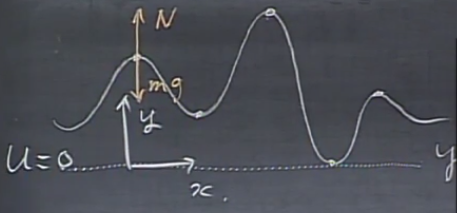
\includegraphics[scale=0.8]{\pIImages/lec13_equilibrium}
\end{center}

The points along the curve have a gravitational potential energy which is $U = m g y$, since we defined $U = 0$ at $y = 0$ (the $= 0$ part is just outside the screen grab above). Since the plot is of $y = f(x)$, for some function $f$, we can also write that $U = m g f(x)$.

There are then points along this curve where $\displaystyle \frac{dU}{dx} = 0$. Those points occur where the curve's slope (or derivative) are zero, by definition, which is at the top of each peak, and at the bottom of each valley, as signified by a dot in the above figure.

From the definition we found before, that then means that $-F_x = 0$, so the net force in the $x$ direction is zero.\\
At such a point, there is a force $-m g$ in the $y$ direction, and a normal force $N = + m g$, so that there is no net force there, either.

Since there is no net force on the object at one of these points, and we can put it in such a situation at rest, it will stay exactly where it is.\\
However, there is an important difference between these two types of points  (peaks and valleys). If we try to balance a marble at the top of such a peak, just about any tiny vibration, small amount of wind etc. will get it moving. Being at the top of a large downwards slope, in either direction, it will then clearly begin to accelerate downwards -- and again, the force is in the direction of decreasing potential energy (which of course is the same thing as being in the \emph{opposite} direction as \emph{increasing} potential energy).

However, if we put a marble in one of the valleys, what happens? If there is a small force, causing a motion in any direction, it will be forced back into the valley. The force is yet again in the direction opposing the increase in potential energy, and potential energy increases both to the left \emph{and} to the right! Therefore, the force is such that the marble is returned to the middle of the valley again, to the point of lowest potential energy.

The difference between these two zero points are that the peaks provide \emph{unstable equilibrium}, while the valleys provide \emph{stable equilibrium}. If there is a disturbance in the first case, it goes out of control. In the second case, in the valleys, any small disturbance is automatically countered, and the object goes back to where it was, at the bottom.

We can find out which of these two cases a point is mathematically, by looking at the second derivative. If the second derivative of potential energy with respect to $x$ is positive, it's a point of stable equilibrium. If it is negative, it's instead a point of unstable equilibrium.

\subsection{Another look at a spring oscillator}

Let's have another look at the oscillation of a mass on a spring, this time from an energy perspective. We know that $\displaystyle U = \frac{1}{2} k x^2$, so a plot of $U(x)$ would be a parabola:

\begin{center}
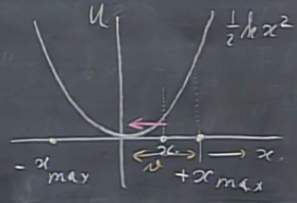
\includegraphics[scale=0.8]{\pIImages/lec13_spring_pe}
\end{center}

Say we have a mass attached to a spring, as usual, and we extend it to $x_{max}$, and let it go, with zero speed.

We know that it will oscillate between $+x_{max}$ and $-x_{max}$, but we can now gain a second insight into this oscillation (albeit one mentioned earlier). Say we release the mass at an extension $x_{max}$ beyond the spring's natural length. That means the potential energy in the spring at that time is

\begin{equation}
U_{initial} = \frac{1}{2} k x_{max}^2
\end{equation}

Since we know that the force will be in the direction opposing the increase in potential energy, the mass will be pulled inwards, towards $x = 0$. Once it crosses the zero point, the force switches directions, since the current \emph{velocity} vector is towards increasing potential energy (the spring is being compressed to be shorter than its natural length). That means the force (and thus the acceleration) instantly flips over, and the mass starts slowing down. The new force is once again in the direction opposing the increase in potential energy, which is again towards $x = 0$, which is now towards the right in the figure.

Because spring forces are conservative (for ideal springs), we can use conservation of energy to write an equation for this system. The \emph{total} energy in the system must equal the spring's stored potential energy at $t = 0$, plus the mass's kinetic energy at $t = 0$. The latter is zero, since we release it at rest (zero speed), so $E_{total} = U_{initial}$. That energy must be held constant -- conservation of energy. Therefore, the sum of the mass's kinetic energy $\displaystyle \frac{1}{2} m v^2$ and the spring's stored energy $\displaystyle \frac{1}{2} k x^2$ must always equal that initial energy. We can set up an equation for this:

\begin{equation}
\frac{1}{2} m v^2 + \frac{1}{2} k x^2 = \frac{1}{2} k x_{max}^2
\end{equation}

This equation must \emph{always} hold for this system, unless there are other forces, such as friction, which we ignore for now.\\
Because $v = \dot{x}$, we can rewrite this equation a bit, by making that substitution, and getting rid of all of the one-halves, and dividing through by $m$:

\begin{align}
\frac{1}{2} m \dot{x}^2 + \frac{1}{2} k x^2 = \frac{1}{2} k x_{max}^2\\
\dot{x}^2 + \frac{k}{m} x^2 - \frac{k}{m} x_{max}^2 = 0
\end{align}

We can then take the time derivative of this. Keep in mind that since the equation is in terms of $x$, we need to use the chain rule for most terms.

\begin{align}
\frac{d}{dt} \left(\dot{x}^2 + \frac{k}{m} x^2 - \frac{k}{m} x_{max}^2\right) = \frac{d}{dt} (0)\\
2 \dot{x} \ddot{x} + 2 \frac{k}{m} x \dot{x} - 0 = 0
\end{align}

We can simplify this equation by dividing through by $2 \dot{x}$:

\begin{equation}
\ddot{x} + \frac{k}{m} x = 0
\end{equation}

Isn't it remarkable? We get the equation for simple harmonic motion, and so we find the same old solutions:

\begin{align}
x        &= x_{max} \cos(\omega t + \varphi)\\
\dot{x}  &= - \omega x_{max} \sin(\omega t + \varphi)\\
\ddot{x} &= - \omega^2 x_{max} \cos(\omega t + \varphi) = -\omega^2 x\\
\omega  )    &= \sqrt{\frac{k}{m}}\\
T           &= \frac{2 \pi}{\omega} = 2 \pi \sqrt{\frac{m}{k}}
\end{align}

\subsection{Motion of a ball along a circular track}

Say we have a circular (or at least semicircular) track of radius $R$. We define $y = 0$ and $U = 0$ to be at the bottom of the track.

\begin{center}
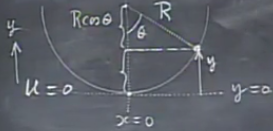
\includegraphics[scale=0.8]{\pIImages/lec13_bowl}
\end{center}

When the ball is at some random location $y$, we can find the angle made with the vertical, $\theta$, via trigonometry.\\
First, we find that the radius $R$ acts as the hypotenuse of a right triangle, where the $x$ component $R \sin \theta$ is at the bottom, and the left side has height $R \cos \theta$. Note that the $y$ coordinate fits $y = R - R\cos \theta$, so that $y = R (1 - \cos \theta)$.

With that in mind, we can write $U$ as a function of the angle $\theta$ now:

\begin{equation}
U = m g y = m g R (1 - \cos \theta)
\end{equation}

Notice that at $\theta = 0$, $U = 0$, as we defined.\\
At $\displaystyle \theta = \frac{\pi}{2}$, $U = m g R$, since it is a height $R$ above $y = 0$.

Using the definition of a radian as the arc length subtended by an angle, where $dS$ is the arc length and $d\theta$ the angle, we find

\begin{align}
\frac{dS}{R} &= d\theta\\
dS &= R d\theta
\end{align}

Taking the time derivative of both sides, we find

\begin{equation}
\frac{dS}{dt} = R \frac{d\theta}{dt} = R \dot{\theta}
\end{equation}

The left-hand term is just the distance moved per unit time, so $\displaystyle \frac{dS}{dt} = v = R \dot{\theta}$.

In most cases, we use $\displaystyle \omega = \dot{\theta} = \frac{d\theta}{dt}$, but in most cases, $\omega$ is also a constant. In this case, it is a function of the angle; the angle will change the fastest near $\theta = 0$ (at the bottom), where the speed is at a maximum, while it will change slower as the ball climbs up the ``edges'' of the circle (I think of it as a ``two-dimensional bowl''), as it is about to come to a halt, and change direction.

As a short aside, we can, as a small-angle approximation, use

\begin{equation}
\cos \theta \approx 1 - \frac{\theta^2}{2}
\end{equation}

This approximation uses the first two terms of a Taylor expansion for $\cos \theta$. If you are unfamiliar with Taylor expansions, you could look them up (even the basics are a bit too much to cover in what is already an aside). In short, they provide for a way to approximate about any function as a polynomial, or -- with an infinite amount of terms -- exactly equal those functions.

Last time we used such an approximation, we used only the first term, $\cos \theta \approx 1$. That's too inexact for this case, though -- we would end up with $U = m g R (1 - 1) = 0$ for all $\theta$!

Even for angles of about 11.5 degrees, the error caused by this approximation is way, way less than 1\% (less than 0.01\%, actually). In fact, for as much as 30 degrees, we have $\cos(\ang{30}) \approx 0.8660254$, while the approximation gives $0.862922$. It's off by about 0.3\% -- still not a lot, all things considered.

Let's return to the problem at hand. Using this approximation, we apply the conservation of mechanical energy to this system. The total mechanical energy must be a constant. If we release the object as zero speed, and thus zero kinetic energy, the total energy (kinetic + potential) must always equal that value:

\begin{equation}
M_E = \frac{1}{2} m v^2 + m g R(1 - \cos \theta)
\end{equation}

Since $v = R \dot{\theta}$, $v^2 = R^2 \dot{\theta}^2$. Let's also apply our approximation for the cosine. What we end up with is

\begin{align}
M_E &= \frac{1}{2} m R^2 \dot{\theta}^2 + m g R(1 - (1 - \frac{\theta^2}{2}))\\
M_E &= \frac{1}{2} m R^2 \dot{\theta}^2 + m g R \frac{\theta^2}{2}
\end{align}

We can now take the time derivative of this. $M_E$ is a constant, so that becomes zero. As far the rest, we use the chain rule again:

\begin{align}
0 &= \frac{1}{2} m R^2 (2 \dot{\theta} \ddot{\theta}) + \frac{m g R}{2} 2 \theta \dot{\theta}\\
0 &= m R^2 \dot{\theta} \ddot{\theta} + m g R \theta \dot{\theta}\\
0 &= R^2 \ddot{\theta} + g R \theta
\end{align}

We can rearrange that as

\begin{equation}
\ddot{\theta} + \frac{g}{R} \theta = 0
\end{equation}

... and it is then again obvious that we have as simple harmonic oscillator! We know the solution to this differential equation, so we can write down

\begin{align}
\theta &= \theta_{max} \cos (\omega t + \varphi)\\
\omega &= \sqrt{\frac{g}{R}}\\
T      &= 2 \pi \sqrt{\frac{R}{g}}
\end{align}

Note that this $\omega$ is completely unrelated to the $\displaystyle \frac{d\theta}{dt}$ we had earlier in the derivation -- it's a good thing we didn't call that $\omega$! This one is a constant, while the other one changed with time.

Note how these equations are identical to the ones for a pendulum, that we derived earlier, also using a small-angle approximation. This time, however, it is our approximation which caused the similarity -- we made the equation quadratic in $\theta$ by doing that. The spring oscillation was quadratic in $x$ from the beginning.

Finally, on to an important detail. Nowhere in this derivation did we consider the normal force from the track on the ball. Is it really safe to ignore it? Why?

It turns out that yes, we can ignore it, because in the case of this circular track, it is always perpendicular to the direction of motion. A force perpendicular to a motion \emph{cannot} do work, because of the definition of the dot product: an angle of $\ang{90}$ between force and displacement always means zero work.

Next, a very interesting demonstration follows, that might cause some sleeplessness until we find the answer to what's going on, likely in two weeks or so.

\section{Lecture 14: Orbits and escape velocity}

As we know, the gravitational force has infinite range. Its strength at a distance is limited, though, due to the inverse square relationship. Because of this, there is a speed, the \emph{escape velocity}, that lets you escape from a body's gravitational field. That is, if you start out with that speed, you will escape it forever, even with no additional outwards force (no engines required). Of course, if you \emph{do} have engines, you certainly don't need to stay above the escape velocity the entire time to get away; all you need to do is overcome the force of the gravitational pull.

We can find this velocity for a given body (such as the Earth) quite easily, using conservation of energy. The kinetic energy at launch must be $\displaystyle \frac{1}{2} m v_{esc}^2$, and since the problem definition is that in never adds to that kinetic energy (no engines). That must therefore be the total energy of the object, at all times. The total energy at any given time is the sum of the kinetic energy at some point $r$, which we call $\displaystyle \frac{1}{2} m v_r^2$, and the potential energy at that point, $\displaystyle - \frac{G M m}{r}$, with $M$ being the mass of the Earth (or the body), and $m$ the mass of the object trying to escape.

\begin{equation}
\frac{1}{2} m v_{esc}^2 + \left(-\frac{G M m}{R_{Earth}}\right) = \frac{1}{2} m v_r^2 + \left(-\frac{G M m}{r}\right)
\end{equation}

On the left side, we have the total energy as we start out our journey, and on the right, the total energy some distance $r$ away.

However, since the goal is for the energy to be enough to escape to an infinite distance, the kinetic energy ``at'' infinity (let's just say extremely, extremely far away, since being ``at'' infinity is meaningless), the potential energy is zero, by definition. The kinetic energy is also zero, \emph{if} we gave it \emph{just} enough energy, and not any more than required (we know that the Earth's gravity will reduce the speed, and thus the kinetic energy, as time goes on).

Because of this, we can set the entire right side of the equation equal to zero, which is valid ``at'' infinity (or just so far away that the gravitational pull of the Earth is now completely negligible), and solve for the escape velocity:

\begin{align}
\frac{1}{2} m v_{esc}^2 -\frac{G M m}{R_{Earth}} = 0\\
v_{esc}^2 -\frac{2 G M}{R_{Earth}} = 0\\
v_{esc} = \sqrt{\frac{2 G M}{R_{Earth}}}
\end{align}

where, again, $M$ is the mass of the Earth. For Earth, this value is then about 11.2 km/s. So if we neglect air resistance, which will surely make these results valid if we are at the Earth's surface, if we could fire a cannon ball at more than 11.2 km/s, it would never fall back to Earth.

If the initial velocity is greater, then you will still have kinetic energy (and thus speed) left when you've escaped. In the case you do ``escape'', with the condition $E_{init} \ge 0$, you are in an \emph{unbound orbit}. In the case that $E_{init} < 0$, you enter a \emph{bound orbit}, and will never escape the gravitational pull of the Earth (or the body in question).

\subsection{Circular orbits}

Elliptical orbits will be covered later in the course, along with Kepler's laws and other fun stuff, but for now, let's introduce circular orbits, as a simplified case.

Say we have a mass $m$ orbiting the Earth, with Earth's mass being $M$, and say that $m \ll M$.\\
It moves in a circle around the Earth at constant (tangential) speed, but not constant velocity -- there is a constant centripetal acceleration, or it wouldn't be moving in a circle. Centripetal acceleration is provided by centripetal force, which in this case is the attractive force of gravity of the Earth on the mass.

We know how to find the gravitational force using the Newton's law of universal gravitation, and we can set that equal to the centripetal force $\frac{m v^2}{r}$ (which is just $a_c m$, via $F = m a$):

\begin{align}
\frac{G M m}{r^2} = \frac{m v_{orbit}^2}{r}\\
\frac{G M}{r} = v_{orbit}^2\\
\sqrt{\frac{G M}{r}} = v_{orbit}
\end{align}

where $r$ is the radius of the orbit, which has nothing to do with the radius of the Earth itself. $v_{orbit}$ is then the tangential speed of the object that is in orbit. Knowing these facts, we can now find the period of the orbit:

\begin{equation}
T = \frac{2 \pi r}{v_{orbit}} = 2 \pi \frac{r^{3/2}}{\sqrt{G M}}
\end{equation}

If we plug in the Sun's mass, and $r = \SI{149.6e9}{m}$, the approximate average distance to the sun, we find Earth's orbital period $T \approx 365.33$ days. Not bad at all, since this is only an approximation (it ignores the several things that matter, including the Earth's elliptical orbit).

As a different example, we can take the space shuttle, or the space station, which orbit at 250-400 km above the Earth's surface. If we make the calculation for 400 km, so that $r = R_{Earth} + 400$ km, we find $v_{orbit} \approx \SI{8}{km/s}$ and $T \approx 90$ minutes(!).

Note that the orbital parameters are independent on the mass of the orbiting object. It only depends on the mass of the object you orbit, and the distance from it (i.e. the radius of the orbit), times some constants.

Also note that $v_{esc} = \sqrt{2} \times v_{orbit}$, for a given point. (In $v_{esc}$, we used the radius of the Earth, because we wanted to calculate the escape velocity from the surface.)

The total mechanical energy at some radius $r$, at orbital velocity $v_{orbit}$, is

\begin{equation}
E = \frac{1}{2} m v_{orbit}^2 - \frac{G M m}{r}
\end{equation}

We can substitute the value for $v_{orbit}^2$ in there, though:

\begin{align}
E = \frac{1}{2} m \frac{G M}{r} - \frac{G M m}{r}\\
E = -\frac{1}{2} \frac{G M m}{r} = \frac{1}{2} U = - K_E
\end{align}

Quite an interesting result. In words, then, the total energy of an orbiting object is always half its gravitational potential energy, and also the negative of its kinetic energy.

Now, for something completely different (more on orbits in a few weeks).

\subsection{Power}

\emph{Power} is energy per unit time -- or work per unit time, since energy and work are closely related, and share the same dimension. The SI unit for power is joules per second, or watts, W; not to be confused with W for the quantity of work! If we have $W = $ something then it's work; if we have $P = 10$ W, then it's watts.

Stated differently, it is then just the derivative of work -- that is, $P = \displaystyle \frac{dW}{dt}$.\\
Since $dW = \vec{F} \cdot \vec{dr}$, we can take the time derivative of both sides:

\begin{equation}
\frac{dW}{dt} = \vec{F} \cdot \frac{\vec{dr}}{dt}
\end{equation}

... and since the rate of change versus time of $\vec{dr}$ is simply the velocity:

\begin{equation}
P = \vec{F} \cdot \vec{v}
\end{equation}

\subsubsection{Power in riding a bicycle}

Let's look at an example: riding a bicycle. We try to keep a constant velocity, which means there should be no net force on the bike. However, there \emph{is} air drag, and the force opposing your motion, $F_{res} \propto k v^2$. In order for there to be no \emph{net} force, your pedaling must then provide an equally great force in the forwards direction, in order for you to keep a constant speed.

As an aside, how does pedaling provide this force? First, you push down on the pedals, and the pedals push back on you with equal force via Newton's third law. This causes no net force on the bike, and we call these forces \emph{internal forces}.

The pedals push on the chain, and the chain pushes on the wheel, all of which cancels, but finally, the wheel now wants to rotate, because of the force exerted by the chain.

The wheel pushes backwards on the ground, which leads to a reaction force such that the ground pushes the wheel forward. Finally something useful! This only works because of friction, of course -- without friction, it would simply start spinning, and there would be no forward force on the bicycle.

Now, let's look at the amount of power you must provide to overcome air resistance. We can model this as a regime II problem, so the drag force is proportional to $k_2 v^2$. Say that the power you must provide at 10 miles/hour is 15 watts -- which is a given, and not something we actually show.

Now, the power we must provide is $P = \vec{F} \cdot \vec{v}$, as we showed earlier. Since the force and the velocity are in the same direction, $P = F v$. Since $F = k_2 v^2$, we find $P = k_2 v^3$! It is proportional not to $v^2$, but $v^3$.

If you then want to speed up to 25 mph, 2.5 times the original speed, you need to provide $2.5^{3} \approx 15.6$ times the power, about 230 watts! For 30 mph, 3 times the original speed, you need $3^3 = 27$ times the power (over 400 watts)! Needless to say, we reach the limits of human physiology rather quickly if we keep going like this. At 50 mph, it would take over 240 times the power (over 1800 watts -- far above what any human could do, except for elite athletes for a period of seconds or less)!

\subsection{Heat energy}

First, a few definitions. We use the symbol $Q$ for heat energy, often in the unit of calories. A calorie is the energy required to raise the temperature of 1 gram of water by 1 degree Centigrade (or 1 Kelvin, which is the same thing). There are, unfortunately, a ton of different definitions for a calorie, but all are close to 4.2 joules. (Some are defined as the energy required to heat 1 g of water from $3.5 {}^\circ$C to $4.5 {}^\circ$C, others from 14.5 to 15.5, 19.5 to 20.5, etc.)

Next, there is the \emph{specific heat} $C$, which is a constant (for a given material) that specifies the amount of energy required to raise the temperature of that material by 1 degree centigrade, per unit mass. That is, it's in $\text{cal}/(g {}^\circ\text{C})$.\\
If we want the unit to use kilograms instead of grams, which is always a nice thing when using the MKS (meter-kilogram-second) system, we simply multiply the constant by 1000.

The amount of heat energy Q, is then

\begin{equation}
Q = m C \Delta T
\end{equation}

in calories, if $m$ is in grams, $C$ in the units stated above (per gram, not per kilogram), and $\Delta T$ in either Kelvin or degrees centigrade (they are equivalent; the zero point is the only difference).\\
As a reference, ice has a specific heat of about 0.5, compared to liquid water's 1. Aluminium has a specific heat of about 0.2, and lead a very low 0.03.

James Joule first found that mechanical work and heat energy are equivalent in 1845, though he was not the first to begin research on the topic. This research, among other things, led to the naming of the joule in his honor.

\subsection{Power and the human body}

The human body radiates heat, infrared radiation, at a rate of about 100 watts -- 100 joules per second. That is about $10^7$ joules per day, which then is about 2.4 (or $\approx 2$) million calories.\\
Clearly, then, we need to input an equivalent amount of energy, or we would run dry sooner rather than later! We get this energy from food, of course.\\
Food labels are usually in kilocalories, which is sometimes written as either Cal (capital c) or kcal. They often mention the equivalent value in kilojoules as well.\\
So when a food label says 400 (kilo)calories, that that is enough for a power output of 100 watts for about 4 hours.

Normal, daily activities use almost no energy at all, compared to the rate of energy use of the body that occurs either way. Walking up 10 meters (vertically) of stairs, 5 times a day, is an average power use of about 1 W, if spread out over over 10 hours or so. That's only about 1\% of the heat energy produced by the body when essentially at rest.

On the other hand, if you climb a mountain of 5000 feet (about 1500 meters), you might do about a million joules worth of mechanical work just to overcome gravity, which is not negligible compared to the $10^7$ joules daily. In other words, you need to eat more, in order to stay the same weight (or mass, rather!).\\
Because the conversion from food energy to mechanical work is quite inefficient, eating 10\% more won't do it, though; you may have to eat 40\%+ more in order to account for the increased energy use.

\subsection{More heat, and electric energy}

Consider taking a bath: we might need to heat 100 kg of water, by about 50 degrees C. (I'm not so sure I agree with that number, though! Even if the water was $0 {}^\circ$C to begin with, it would probably be painfully hot! Anyway, let's work with the number from the lecture.)

With $C = 1 \text{ cal/(g} {}^\circ \text{C})$ for water, the answer is then simply the mass (in grams!) times $C = 1$ times 50 degrees $C$, or about $5 \cdot 10^6$ calories, which is about $\SI{2e7}{J}$.

It's fairly difficult to produce 120 watts of work in turning a crank on a generator that then produces electric energy; a student was unsuccessful, and the professor says he is also unable to do so. Still, you would need to produce those 120 watts for 48 hours in order to heat up the water in that bath by 50 degrees!

Next, a demonstration of a simple battery is shown; four cells consisting of a zinc anode and a copper cathode in a sulfuric acid solution are wired in series to power a small light bulb.

After that, some more numbers: the global energy consumption (in 1999, when the lectures were recorded) is/was about $\SI{4e20}{J}$ per year.\\
The USA consumes about 1/5 of that, with 1/30 of the world's population.

The Sun has a power output of about $\SI{4e26}{W}$, radiated in mostly visible light and infrared. Of course, it radiates a roughly equal amount in all directions, so only a small fraction of that reaches the Earth. We can calculate how large Earth's cross section is, and find the ratio of that divided by $4 \pi R^2$, with $R$ being the mean distance between the Earth and the Sun. We find about 1400 watts per square meter, that reaches the Earth's atmosphere.\\
The measured value at the ground varies greatly, for many reasons: the Sun's altitude above the horizon (i.e. day/night cycle, seasons, location on the Earth), cloud cover, and more.

If we try put solar panels on a horizontal roof, then clearly they will not do anything useful when the sun is just at the horizon.

Taking all this into account, along with solar cell inefficiency, we could perhaps provide enough energy to power the planet continuously by having a 400 mile by 400 mile solar grid -- not a small area! That area is three times that of England. Clearly, we cannot sustain our current energy use by solar power alone.

Lecture question time:\\
``When the sun is in the zenith and the sky is perfectly clear, the solar power we receive on the surface of the earth is roughly 1 kW per square meter (on a horizontal surface that is normal to the direction of the sun).

Calculate the average solar power per square meter (in Watts) on a horizontal surface for a day when the sun goes through the zenith at noon.

The sun goes through the zenith exactly twice a year on latitudes that are close to the equator. Take the angle to the sun into account.''

Okay, let's see. Let's imagine one single square meter somewhere on the Earth. First we have sunrise, where the sun is at $-\pi/2$ radians compared to the zenith. At noon, it is at 0 rad (straight above), and at sunset, at $+\pi/2$ radians. The power at a given angle $\theta$ should be $P = (\SI{1000}{W})\cos\theta$. Next, we need to find an average.

We can do find the average by an integral:

\begin{equation}
\overbar{P} = \frac{1}{b - a} \int_a^b 1000 \cos \theta d \theta
\end{equation}

where $a = -\pi/2$ and $b = \pi/2$. However, that is only exactly half a day -- the other 12 hours, there is zero sunlight, so we need to divide our answer by two, which causes the additional factor of 1/2 below. We find

\begin{align}
1000 \frac{1}{\pi} \frac{1}{2} \int_{-\pi/2}^{\pi/2} \cos \theta d \theta &= \frac{1000}{2 \pi} \int_{-\pi/2}^{\pi/2} \cos \theta d \theta = \frac{1000}{2\pi} \Big[ \sin \theta \Big]_{-\pi/2}^{\pi/2}\\
                                                              &= \frac{1000}{2\pi} \times 2 = \frac{1000}{\pi} \approx \SI{318.3}{W}
\end{align}

I do believe I'm missing a simplification, but at least this gets us the correct answer.

Finally, a small note on the current energy crisis.\\
We are using fossil fuels at a rate which is about one \emph{million} times greater than nature's production. At this rate, we will run out in less than 100 years. Fossil fuels account for a bit over 80 percent of human energy consumption, so clearly we need to start producing a \emph{lot} of energy from other sources, or we will simply run out. While solar power is very useful, we have already ruled it out as a full replacement. We can combine many energy sources, though, and have solar power be one of them.

Nuclear fusion is often touted as the ``energy source of the future''. And indeed, if we can create an efficient reactor (current designs are not usable in practice, and mostly use more power than they provide back), it could provide practically limitless energy. One possible fuel source is deuterium and tritium, isotopes of hydrogen, present in sea water. We have enough water to provide the current world's energy usage for about 25 billion years, so if it could work, the energy problem would be solved.

Not only that, but fusion is both clean and intrinsically safe. Most of us know of Chernobyl or Fukushima -- rare accidents, but they do happen, and can be very problematic.\\
(Though as of late 2013, the death toll due to Fukushima is still zero (but the lifetime rate of cancer has likely increased in some people), and fission energy has a lower death rate per unit energy produced than even wind and solar energy. I'm not trying to sell some propaganda here, but I do feel that nuclear fission has a worse reputation than it deserves, even though there obviously are risks.)

If a tsunami or an earthquake were to hit a \emph{fusion} reactor, however, not a lot can happen. In magnetic containment fusion, the magnetic field would collapse if power was cut, and the reactor would automatically shut down. Not automatically as in a safety protocol, but rather without the containment, the reaction cannot be sustained, and stops all by itself. That's in contrast with a fission reactor, which must rely on safety measures to stop the reaction, so that it doesn't go out of control.\\
(Newer fission reactor designs are safer than ones in use, but few new designs are actually put into use, likely in part due the rather vocal opposition to nuclear energy.)\\
In addition, a fission reactor usually has many tons of fuel inside, while a fusion reactor can be powered off just grams of fuel, and use well below 1 ton of fuel in a year -- and the fuel is just hydrogen isotopes. Granted, tritium is radioactive, and there are some radioactive byproducts, but nowhere near the many tons a year of poisonous, radioactive material that fission reactors produce per year.


\section{Lecture 15: Momentum and its conservation}

We will now introduce the concept of momentum.\\
Momentum is a vector: the product of mass and velocity. The SI units are then kg $\cdot$ m/s or N $\cdot$ s; there is no named unit for this quantity.

It is usually written as $\vec{p}$, so

\begin{equation}
\vec{p} = m \vec{v}
\end{equation}

Momentum is closely connected with force, and knowing the above, it is easy to show how. $\displaystyle F = m a = m \frac{dv}{dt}$. We can work backwards, assuming $m$ is a constant so that $m \frac{dv}{dt} = \frac{d(mv)}{dt}$:

\begin{equation}
F = m \frac{dv}{dt} = \frac{d(mv)}{dt} = \frac{dp}{dt}
\end{equation}

So force is the time derivative of momentum.\\
This also implies that in order for an object's momentum to change, a force must have acted on it. And, conversely, if a (net) force acts on an object, its momentum must change.

Next, the professor shows (in some detail) how momentum is conserved for a \emph{system} of particles/objects, unless there is a net \emph{external} force on them. What happens internally does not matter, since all such internal forces cancel out, when you consider the system as a whole. For example, if two particles collide, the momentum of both particle \#1 and of particle \#2 may change, but the momentum of \#1 + \#2 will stay a constant.

This then leads to the \emph{conservation of momentum}, which is a very helpful concept in solving some kinds of problems. Let's solve a simple problem using this principle.

Say we have two objects of masses $m_1$ and $m_2$ respectively, both moving towards the right, with velocities $v_1$ and $v_2$, where $v_1 > v_2$. Eventually, the two will collide.

Momentum prior to the collision can be found by the sum $m_1 v_1 + m_2 v_2$; since it is a vector, it has a direction. Both velocities are towards the right, so the net momentum will be as well; we take right to be increasing value of $x$, so that the numbers are positive.

In the collision, the masses will stick together -- pretend that we put glue on one of them. (Collisions where the two separate after colliding are covered later in the lecture, or in the next.)\\
Because they stick together, they will share a velocity later -- and a momentum, as well. The momentum after the collision can be written as $(m_1 + m_2) v'$, if we call the new velocity $v'$. 

Via conservation of momentum, the two must be equal, if there are no external forces (so this collision happens on a frictionless table, with no air drag etc). We set them equal, and solve for $v'$:

\begin{align}
(m_1 + m_2) v' &= m_1 v_1 + m_2 v_2\\
v' &= \frac{m_1 v_1 + m_2 v_2}{m_1 + m_2}
\end{align}

To get a feeling for this, say $m_1 = \SI{1}{kg}$, $m_2 = \SI{2}{kg}$, $v_1 = \SI{5}{m/s}$ and $v_2 = \SI{3}{m/s}$. Mass 1 has a momentum of $\SI{5}{kg m/s}$, while mass 2 has $\SI{6}{kg m/s}$. The net momentum prior to the collision is then $\SI{11}{kg m/s}$, since the two are in the same direction.

Both velocities are towards the right and thus positive, so $v'$ will also be positive.\\
Plugging the numbers in, we find $\SI{11/3}{m/s}$ as the new velocity for the masses, moving together.

What is now the momentum? It is the new velocity times the total mass, which is $(11/3) \times 3$, so indeed we find that momentum was conserved. Not a huge surprise, since we derived the equation from that assumption!

What may be surprising is instead what happens to the kinetic energy.\\
Prior to the collision, the total kinetic energy was 12.5 J + 9 J = 21.5 J.

After the collision, the total kinetic energy is only $20.1\overbar{6}$ J -- we lost one and a quarter of a joule. Not a whole lot, perhaps, but let's look at a second situation.

Say we have the same values for the masses and velocities, only that $v_2$ is now negative, i.e. to the left, and so the two hit each other head-on.

Mass 1 still has the same momentum of $\SI{5}{kg m/s}$, but $v_2$ now has $-\SI{6}{kg m/s}$. The net momentum is now $\SI{-1}{kg m/s}$ instead of +11.

Using the same formula, we now find $v' = -1/3$ m/s. The initial kinetic energy is unchanged -- the masses are the same, and the \emph{speeds} are the same -- but the kinetic energy after the collision is now a tiny 1/6 of a joule!

In short: in the absence of (net) external forces, the momentum of a \emph{system} of two or more objects is always conserved; kinetic energy, however, is not.

Let's have a look at a two-dimensional problem from a lecture question:

``In a scattering experiment, an incident alpha particle of mass $M_1 = 4u$ interacts with a static proton of mass $M_2 = u$. The incident particle is initially moving along the x-axis with a velocity $\vec{v_1} = v_{1x} \hat{x} = 0.05 c \hat{x}$, and a final velocity (after collision) $\vec{v_1}' = v_{1x}^{'} \hat{x} + v_{1y}^{'} \hat{y} = 0.044 c \hat{x} + 0.008 c \hat{y}$, where $c$ is the speed of light ($c = \SI{3e8}{m/s}$).

What is the speed of the proton after the collision?\\
What is the direction of the proton after the collision? (give the angle with respect to the x-axis in radians)''

To solve this, we apply conservation of momentum on the two axes, independently of each other.\\
Before and after the collision, in the $x$ direction:

\begin{align}
4 u v_{1x} = 4 u v_{1x}^{'} + u v_{2x}^{'}\\
4 (v_{1x} - v_{1x}^{'}) = v_{2x}^{'}
\end{align}

where $v_{2x}^{'}$ is the $x$ component of the proton's velocity after the collision. Plugging in the numbers given, we find $v_{2x}^{'} = 4(0.05c - 0.044c) = 0.024c$.

Next, the $y$ direction. Neither particle has any $y$ component whatsoever at the moment, so the net momentum prior to the collision is clearly zero. That also means that the net momentum \emph{after} the collision must be zero.

\begin{align}
4 u v_{1y}^{'} + u v_{2y}^{'} = 0\\
v_{2y}^{'} = -4 v_{1y}^{'}
\end{align}

So we find $v_{2y}^{'} = -0.032c$.

With that in mind, we can now calculate the speed as $v_2^{'} = \sqrt{(v_{2x}^{'})^2 + (v_{2y}^{'})^2} = 0.04c$.

Next up, the angle made with the $y$ axis. If we consider the components, it must be angled downwards to the height. Drawing it out, we find that

\begin{equation}
\theta = \arctan \frac{v_{2y}^{'}}{v_{2x}^{'}} = \arctan \frac{-0.032}{0.024} = \ang{-53.13}
\end{equation}

This angle would put it in the correct quadrant, and since the magnitude of the $y$ component is slightly greater than that of the $x$ component, it makes sense that the angle is a bit more than a 45 degrees down from the axis.


\subsection{Center of mass}

Every object, regardless of shape or size, has a center of mass; a single point, which has some very interesting and useful properties.

We take any object, of any size (greater that zero, however, or the entire point is lost), and think of it as being composed by a practically infinite amount of small masses $m_i$. Each mass has a position vector $\vec{r_i}$ from the origin, which we are free to choose.

\begin{figure}[H]
  \centering
\begin{tikzpicture}
\node [cloud, draw,cloud puffs=10,cloud puff arc=120, aspect=2, inner ysep=2em] at (4, 2) {};

\coordinate (P1) at (0.5,0.3);
\coordinate (P2) at (3.2,2.2);
\coordinate (P3) at (4.5,1.8);

\draw[thick] (0,0) circle [radius=2mm];
\fill[black] (P1) circle (0.7mm);
\draw[thick, ->] (P1) -- (P2) node[midway, above=1mm] {$\overline{r}_i$};
\draw[thick, red, ->] (P1) -- (P3) node[midway, below=1.5mm] {$\overline{r}_{cm}$};
\draw[thick] (P2) circle [radius=1mm] node[above=2mm] {$m_i$};
\draw[thick, red] (P3) circle [radius=1mm] node[above=2mm] {$cm$};
\end{tikzpicture}
\end{figure}


It is then true that the 

\begin{align}
M_{tot} \vec{r_{cm}} &= \sum_i m_i \vec{r_i}\\
\vec{r_{cm}} &= \frac{1}{M_{tot}} \sum_i m_i \vec{r_i}
\end{align}

In the limit as the masses become infinitesimally small, this becomes an integral:

\begin{align}
\vec{r_{cm}} &= \frac{1}{M_{tot}} \int \vec{r} \mathop{dm}
\end{align}

$x$, $y$ and $z$ components of this can be found in the same way, with three separate integrals.

For the simple case of two particles along a single axis:

\begin{equation}
x_{cm} = \frac{m_1 x_1 + m_2 x_2}{m_1 + m_2}
\end{equation}

This gives a result where the center of mass is closer to the more massive of the two objects. If they are equally massive, the center of mass is at the midpoint between the two.

Returning to the first equation solved for $\vec{r_{cm}}$, we can take the time derivative of both sides of this equation. $\vec{r_{cm}}$ becomes $\vec{v_{cm}}$, and $\vec{r_i}$ becomes $\vec{v_i}$, since velocity is the time derivative of position.

\begin{equation}
\vec{v_{cm}} = \frac{1}{M_{tot}} \sum_i m_i \vec{v_i}
\end{equation}

However, note that $\sum_i m_i \vec{v_i}$ is the sum of the mass-velocity products: it is the total momentum of the system. In other words,

\begin{align}
\vec{v_{cm}} &= \frac{1}{M_{tot}} \vec{p_{tot}}\\
\vec{p_{tot}} &= M_{tot} \vec{v_{cm}}
\end{align}

This second result is an important one: the total momentum of a system can be found by knowing its total mass and the velocity of its center of mass, and is the same regardless of what the rest of the system is doing.

Not only that, but we can take the time derivative of this. The time derivative of momentum is force (or net external force, to be more precise), while the derivative of velocity of the center of mass is the \emph{acceleration} of the center of mass:

\begin{equation}
F_{ext} = M_{tot} \vec{a_{cm}}
\end{equation}

This is a very interesting result. Regardless of the shape of an object, if we know the external force and the total mass, we can predict how the center of mass moves in a simple way, even though the motion of the object as a whole may be very complicated and involve tumbling/spinning at varying speeds, etc.

So if the (net) external force is zero, the center of mass will continue to move in a straight line, forever, regardless of what the rest of the object is doing.

\section{Lecture 16: Elastic and inelastic collisions}

Last lecture was focused on inelastic collisions; we will now consider general collisions, including elastic ones. Again, let's start with a one-dimensional example.

A mass $m_1$ is moving towards the right with speed $v_1$, towards a mass $m_2$ which is at rest. We take increasing values of $x$ to be towards the right.

After the collision, $v_1^{'}$ can be either positive or negative (to the right or to the left), while $v_2^{'}$ is certainly towards the right. (If an object hits it from the left, how could it start moving towards the left?)

To find the velocities after the collision, we can apply conservation of momentum. Only the first mass had any momentum prior, so that must be the sum of the momentum after the collision as well:

\begin{equation}
m_1 v_1 = m_1 v_1^{'} + m_2 v_2^{'}
\end{equation}

Unfortunately, the equation has two unknowns; we need a second equation to get anywhere.

In order to find a second equation, we can use the conservation of energy. \emph{Kinetic} energy is not necessarily conserved in collisions, which we saw last lecture. However, the kinetic energy that is lost must be converted to some other form of energy, such as heat energy.

If we use an extra $Q$ to denote the rest of the energy, we can write an equation of the form $K + Q = K'$, where $K$ is the kinetic energy prior to the collision, and $K'$ is the kinetic energy after.

There are three possible cases here.

\begin{itemize}
\item $Q > 0$: we call this a \emph{superelastic} collision; the amount of kinetic energy has \emph{increased} (as demonstrated with a spring's stored energy as the source in the previous lecture; an explosion or such could also cause this to happen).
\item $Q = 0$: this is an \emph{elastic} collision (or ``completely elastic''; the modifier ``completely'' is really not necessary, however). Kinetic energy is \emph{conserved} in this special case.
\item $Q < 0$: this is an inelastic collision. Kinetic energy is lost in the collision (in any amount from almost none lost, to \emph{all} kinetic energy lost), and is mostly turned into heat (but perhaps also noise and vibration, etc).
\end{itemize}

Let's focus on the special case of elastic collision, so that $Q = 0$ and $K = K'$. In this case, we can write an equation relating the initial kinetic energy to the final kinetic energy, as follows:

\begin{align}
\frac{1}{2} m_1 v_1^2 &= \frac{1}{2} m_1 (v_1^{'})^2 + \frac{1}{2} m_2 (v_2^{'})^2\\
m_1 v_1^2 &= m_1 (v_1^{'})^2 + m_2 (v_2^{'})^2
\end{align}

Combining this with the equation that relates the momentum of the system, we can find expressions for $v_1^{'}$ and $v_2^{'}$ as follows, by solving the system of equations:

\begin{align}
v_1^{'} &= \left(\frac{m_1 - m_2}{m_1 + m_2}\right) v_1\\
v_2^{'} &= \left(\frac{2 m_1}{m_1 + m_2}\right) v_1
\end{align}

So the above is valid under three conditions: the initial velocity $v_2 = 0$ initially, $Q = 0$ and momentum is conserved (i.e. there is no net external force on the system).

We will now look at what will happen in three special cases: $m_1 \gg m_2$, $m_1 \ll m_2$ and $m_1 = m_2$.

First out is $m_1 \gg m_2$, which turns out to be the same as $m_2 \to 0$. What happens in the above equations as $m_2 \to 0$?

Well, $v_1^{'} = v_1$ -- which comes as no surprise. If a very massive object runs in to one that has practically zero mass, it will just continue on its way.\\
What happens to the smaller object is more interesting: its velocity goes to $v_2^{'} = 2 v_1$. As long as $m_1 \gg m_2$, no matter what the actual masses or velocities are, it will zoom away at twice the speed of the object that hits it.

Next, the opposite case, where $m_1 \ll m_2$, which means $m_1 \to 0$. Since $m_1$ is the one that moves initially, I would expect it to change direction and move backwards at some speed, while $m_2$ does almost nothing. Let's plug it in: we find $v_1^{'} = -v_1$ and $v_2^{'} = 0$, as predicted. It turns out that $m_1$ simply bounces back with the \emph{same} speed, only in the opposite direction. Considering what happened to the tiny mass in the previous case, this might not be obvious -- it was twice the speed in the previous case!

Finally, what happens if the masses are about the same? Plugging it in, we find $v_1^{'} = 0$, and $v_2^{'} = v_1$: the first object stops, and the second moves as the first one did prior to the collision.\\
Most have seen this in action, perhaps while playing pool, or in a ``Newton's cradle'' where several balls (usually at least 3, but 2 works) hang suspended as pendula; you raise one up, and when it whacks on the rest, only the one at the other end starts moving; the others merely ``relay'' the momentum through until it reaches the last ball.

The cases where $m_1 = m_2$ and $m_1 = 0.5 m_2$ are then demonstrated, with very convincing results!

What if $v_2 \neq 0$? More specifically, $v_2 > 0$, so that they are both moving towards the right, with $v_1 > v_2$ so that they will eventually collide. Again, we assume an elastic collision.

If we set up the system of equations, with the change that both masses now have momentum towards the right, and both have initial kinetic energy, we find 

\begin{align}
v_1^{'} &= \frac{m_1 v_1 - m_2 v1 + 2 m_2 v_2}{m_1 + m_2}\\
v_2^{'} &= \frac{2 m_1 v_1 - m_1 v_2 + m_2 v_2}{m_1 + m_2}
\end{align}

With $m_1 = m_2$, this yields a funny result: the two essentially trade speeds with one another. $v_1^{'} = v_2$ and $v_2^{'} = v_1$.

\subsection{Elastic collisions seen from the frame of the center of mass}

We can choose our reference frame such that the center of mass has zero velocity in our frame. This is referred to as the ``center of mass frame'', ``center of momentum frame'' or COM frame.

In this frame, total momentum is always zero. We found last lecture that $\vec{p_{tot}} = M_{tot} \vec{v_{cm}}$, and \emph{in the COM frame}, $v_{cm} = 0$ by definition. That definition is what makes it the COM frame.

Using the definition for the velocity of the center of mass

\begin{equation}
v_{cm} = \frac{1}{M_{tot}} \sum_i m_i v_i = \frac{\sum_i m_i v_i}{\sum_i m_i}
\end{equation}

and a Galilean transformation for the velocities of two particles,

\begin{align}
u_1 &= v_1 - v_{cm}\\
u_2 &= v_2 - v_{cm}
\end{align}

where the $u$ notation is used for the particle's velocities in the COM frame, we can show that the total momentum must be zero in this frame, in a different way.

The sum $\sum_i m_i u_i$ is the net momentum in the COM frame. $u_i = (v_i - v_{cm})$, so we substitute that in and find $\sum_i m_i (v_i - v_{cm})$ as the total momentum. Using the definition of $v_{cm}$ above, that is

\begin{equation}
\sum_i m_i \left(v_i - \frac{\sum_i m_i v_i}{\sum_i m_i}\right) = \sum_i m_i v_i - \sum_j m_j \frac{\sum_j m_j v_j}{\sum_j m_j} = 0
\end{equation}

The denominator in the fraction becomes $1$, and we then have the subtraction of two equal quantities that equals the total momentum, as seen from the COM frame, since the indices $i$ and $j$ are equivalent.

Now that we can hopefully accept the above as being true (I had trouble seeing it until I did the above)...\\
Say we are in this frame, and there are two particles with velocities inward toward the center of mass; one mass $m_1$ with speed $u_1$, and one mass $m_2$ with speed $u_2$ -- again with those speeds being in the COM frame. Also say $Q = 0$ for this collision, i.e. it is an elastic collision.

Momentum is zero both before and after the collision. In addition, because this is an elastic collision, we can also write down an equation relating kinetic energy before and after the collision. Altogether, we have:

\begin{align}
m_1 u_1 + m_2 u_2 &= 0\\
m_1 u_1^{'} + m_2 u_2^{'} &= 0
\end{align}
\begin{equation}
\frac{1}{2} m_1 u_1^2 + \frac{1}{2} m_2 u_2^2 = \frac{1}{2} m_1 (u_1^{'})^2 + \frac{1}{2} m_2 (u_2^{'})^2
\end{equation}

With all this information, we can find (through some tedious algebra) two very simple answers: $u_1^{'} = -u_1$ and $u_2^{'} = -u_2$.

That is, \emph{as seen from the center of mass frame}, which is moving, both simply reverse direction, but keep moving at the same speed. This happens regardless of the masses and speeds, so this is clearly only possible in this very special frame.

In this simple case with only two objects, the definition we have above for $v_{cm}$ is fairly simple:

\begin{equation}
v_{cm} = \frac{m_1 v_1 + m_2 v_2}{m_1 + m_2}
\end{equation}

We can then follow the process of first transforming our velocities into velocities as seen from the center-of-mass by subtracting $v_{cm}$, do the collision calculations knowing that momentum is zero both before and after the collision (this holds for all collisions; inelastic, elastic and superelastic), and then transforming back to the external frame by \emph{adding} $v_{cm}$ back.

Since the center of mass moves at a constant velocity in the absence of external forces, we need not worry about it having changed during the collision (unless we are making an incorrect assumption that the external forces are zero).

Let's try an example (from a lecture question).

``Before a 1-dimensional collision, two masses $m_1 = 3$ kg and $m_2 = 5$ kg have velocities $v_1 = -5$ m/s and $v_2 = 3$ m/s with respect to their center-of-mass frame.

What are their velocities (in m/s) in the laboratory frame after an elastic collision? (The velocity of the center of mass is $v_{cm} = 2$ m/s)''

Alright, so in the center of mass frame, $v_1^{'} = 5$ m/s and $v_2^{'} = -3$ m/s, since all they do in that frame is reverse direction. To convert this to the lab frame, we need to \emph{add} $v_{cm}$ to these numbers, so we find 7 m/s and -1 m/s, respectively. That was certainly very easy.

\subsection{Inelastic collisions seen from the center of mass frame}

The center of mass frame has another interesting property. In the case of a completely inelastic collision, i.e. the two masses that collide stick together, both velocities go to zero (as seen from the center of mass; this would be true even if they were sliding together according to an outside observer).\\
Zero velocity means zero kinetic energy, so \emph{all} kinetic energy will be lost in this frame.

This kinetic energy, as seen from the center of mass frame, is called the \emph{internal energy}; it is the maximum energy that can be converted to heat in a collision.

Let's first calculate the amount of kinetic energy lost in a completely inelastic collision, as seen from the ``lab frame'' (one that is fixed to the room you're in, i.e. what at least I personally would consider the default frame).

We take the case where a mass $m_1$ moves with speed $v_2$ towards a second mass, $m_2$, that is at rest (with respect to the lab frame). It's a completely inelastic collision, so they stick together after the collision.

After the collision, we call the velocity $v'$ (which is just a speed in the same direction as $v_1$, since momentum is conserved), and the total mass is then $m_1 + m_2$.\\
Conservation of momentum gives

\begin{equation}
m_1 v_1 = (m_1 + m_2) v'
\end{equation}

\begin{equation}
v' = \frac{m_1 v_1}{m_1 + m_2}
\end{equation}

$v_{cm} = v'$; that can be seen very easily by looking at the equation for $v_{cm}$, and considering the case where $v_2 = 0$, as it is here. $v_{cm}$ equals exactly the above expression in that case.

Next, we can calculate the difference is potential energy before ($K$) and after ($K'$) the collision. This is the $Q$ we had in a previous equation (see the note just below; I made a small mistake):

\begin{align}
Q = K' - K &= \frac{1}{2} m_1 v_1^2 - \frac{1}{2} (m_1 + m_2) \left(\frac{m_1 v_1}{m_1 + m_2}\right)^2\\
           &= \frac{1}{2} m_1 v_1^2 - \frac{m_1^2 v_1^2}{2(m_1 + m_2)}\\
           &= \frac{m_1 v_1^2(m_1 + m_2)}{2(m_1 + m_2)} - \frac{m_1^2 v_1^2}{2(m_1 + m_2)}\\
           &= \frac{m_1 v_1^2(m_1 + m_2) - m_1^2 v_1^2}{2(m_1 + m_2)}\\
           &= - \frac{m_1 m_2}{2(m_1 + m_2)} v_1^2 \text{ (see below re: minus)}
\end{align}

Phew! This is then, from the external reference frame, the amount of kinetic energy lost in the collision.\\
As it turns out, I accidentally calculated $K - K'$ instead. The only difference is a minus sign, of course, so the actual answer should be \emph{minus} what I actually found; I added the sign in the last step above, instead of re-writing the code for this mess; sorry about that.\\
So the last line in the equation above is correct.

Next, we do the same calculation in the center of mass frame. We know $v_{cm}$, $v_1$ and $v_2$, so we can jump straight to converting the velocities. Using $u_i$ for the velocities as seen from the center of mass frame,

\begin{align}
u_1 &= v_1 - v_{cm} = v_1 - \left(\frac{m_1 v_1}{m_1 + m_2}\right)\\
u_2 &= v_2 - v_{cm} = - \left(\frac{m_1 v_1}{m_1 + m_2}\right)
\end{align}

The first equation simplifies:

\begin{align}
u_1 &= \frac{v_1(m_1 + m_2) - m_1 v_1}{m_1 + m_2}\\
u_1 &= \frac{v_1 m_1 + v_1 m_2 - m_1 v_1}{m_1 + m_2}\\
u_1 &= \frac{v_1 m_2}{m_1 + m_2}
\end{align}

And we can then write them as

\begin{align}
u_1 &= \left(\frac{m_2}{m_1 + m_2}\right) v_1\\
u_2 &= - \left(\frac{m_1}{m_1 + m_2}\right) v_1
\end{align}

We can then calculate the total kinetic energy \emph{prior} to the collision as

\begin{align}
K &= \frac{1}{2} m_1 u_1^2 + \frac{1}{2} m_2 u_2^2\\
K &= \frac{1}{2} m_1 \left(\left(\frac{m_2}{m_1 + m_2}\right) v_1\right)^2 + \frac{1}{2} m_2 \left(- \left(\frac{m_1}{m_1 + m_2}\right) v_1\right)^2\\
K &= \frac{1}{2} m_1 \left(\frac{v_1 m_2}{m_1 + m_2}\right)^2 + \frac{1}{2} m_2 \left(\frac{v_1 m_1}{m_1 + m_2}\right)^2\\
K &= \frac{v_1^2 m_1 m_2^2}{2(m_1 + m_2)^2} + \frac{v_1^2 m_2 m_1^2}{2(m_1 + m_2)^2}\\
K &= \frac{v_1^2 m_1 m_2^2 + v_1^2 m_2 m_1^2}{2(m_1 + m_2)^2}\\
K &= \frac{(m_1 + m_2) m_1 m_2 v_1^2}{2(m_1 + m_2)^2}\\
K &= \left(\frac{m_1 m_2}{2(m_1 + m_2)}\right) v_1^2
\end{align}

Again, phew! Note that this is exactly the same as the answer we found earlier, for the kinetic energy lost in the lab frame.\\
In this frame, that energy is \emph{all kinetic energy that exists to begin with}. After the collision, kinetic energy will be zero, since the wreck sticks together (this entire section is about a completely inelastic collision), and neither body will move with respect to the center of mass after the collision.\\
In other words, the \emph{change} in kinetic energy is the same in both reference frames, even though the initial and final energies are different in the different frames.

Lecture question time.

``Just before an inelastic head-on collision, two cars have a relative speed of $v = 40$ km/h (25 mph). The cars have masses $m_1 = 1300$ kg and $m_2 = 1600$ kg.\\
How much kinetic energy is lost during the collision?''

Hmm. Well, we can use the equation above. Assume $v_2 = 0$, and then it's just a matter of sticking the numbers in there, which yields about 44300 J.

\section{Lecture 17: Momentum of individual objects}

Previously, we measured the speed of a bullet, simply by measuring how long it took the bullet to move a certain distance. This was only possible because of the electronic timer, which both started and stopped automatically, as the bullet was shot through two wires.\\
We will now calculate the speed, by a more manual, indirect method, of firing the bullet into a block hanging as a pendulum. This way, we can find the velocity (with a fairly large uncertainty, but still) with nothing but a small meter stick and knowledge of physics.

The way in which we do this is fairly complex, but let's start simple. We have a solid block of mass $M$ hanging from a string of length $\ell$; this forms a \emph{ballistic pendulum}.

The bullet of mass $m$ comes in with a velocity $v$, and ``merges'' with the block (gets stuck inside), so we can model this is a completely inelastic collision. The block moves from its equilibrium position (straight down), towards the right and slightly upwards (since it is a pendulum!), with velocity $v'$.

We can apply conservation of momentum to find $v'$:

\begin{align}
m v &= (m + M) v'\\
v' &= \frac	{m v}{m + M}
\end{align}

Soon thereafter, $v'$ will have gone to zero, as the pendulum reaches its highest point. Here, we know that kinetic energy is zero, and all kinetic energy has been converted into gravitational potential energy.\\
If we define $U = 0$ at the equilibrium position, the change in gravitational potential energy was $(m + M) g h$, where $h$ is the amount the block moved upwards. This energy must have come from the kinetic energy, so via conservation of energy, we can relate the block's initial kinetic energy (as the bullet is absorbed) and the gravitational potential energy as it stops:

\begin{equation}
\frac{1}{2} (m + M) (v')^2 = (m + M) g h
\end{equation}
\begin{equation}
v' = \sqrt{2 g h}
\end{equation}

With this in mind, we could theoretically fire a bullet into the block, measure how far it moves up, and calculate the speed of the bullet. However, the upwards movement is minuscule, less than a single millimeter; we still cannot measure that with any useful accuracy. We \emph{can} measure how far it travels towards to the side, though, since that excursion is must greater. (Remember how we even neglected the upwards motion of a pendulum completely when we derived an equation for it using simple harmonic motion?)

So if we set the origin at the equilibrium position, we can call the maximum horizontal displacement of the pendulum $x$. Via trigonometry, we can find that $x = \ell \sin \theta$, and $h = \ell - \ell \cos \theta = \ell(1 - \cos \theta)$.

Using the same small-angle approximations we have used previously, that $\displaystyle \cos \theta \approx 1 - \frac{\theta^2}{2}$ and $\sin \theta \approx \theta$ (both only valid for radians), $\displaystyle h \approx \ell \frac{\theta^2}{2}$.

For $\ell = 1$ meter and $\theta = \ang{2}$, we find that $h \approx 0.6$ mm, far to small to measure with any useful accuracy. However, $x \approx \ell \theta \approx 3.5$ cm, which is much more reasonable. 

Since we now know $x$ as a function of $\theta$, we can write $h$ as a function of $x$ by combining the two equations:

\begin{equation}
h \approx \ell \frac{\theta^2}{2} \approx \frac{\ell}{2} \left(\frac{x}{\ell}\right)^2 = \frac{x^2}{2 \ell}
\end{equation}

With this in mind, we can find $v'$ as a function of $x$

\begin{equation}
v' = \sqrt{2 g} (\frac{x}{\sqrt{2 \ell}}) = x \sqrt{\frac{g}{\ell}}
\end{equation}

... and then finally the bullet's original velocity $v$ as a function of $v'$, by using the old conservation of momentum equation we had:

\begin{equation}
v = \frac{v'(m + M)}{m} = x \frac{m + M}{m} \sqrt{\frac{g}{\ell}}
\end{equation}

Let's now look at some numbers. The mass of the bullet is $m = \SI{2.0(2)}{g}$; $M = \SI{3.20(2)}{kg}$, and $\ell = \SI{1.13(2)}{m}$.

With these numbers, we find $v = 4.7 \times 10^{3} x$. The total uncertainty is somewhere around 15\%, in large part because of the large uncertainty in $m$.

When the experiment is carried out, $x \approx \SI{5.2}{cm}$ = 0.052 meters, so $v \approx \SI{244}{m/s}$. Of course, with a 15\% uncertainty, that last four may be rather meaningless. 15\% less than this is just 207.5 m/s, and 15\% more is 280.5 m/s.

Comparing the initial kinetic energy of the bullet $\displaystyle \frac{1}{2} m v^2 \approx 59.5$ J (with a large uncertainty) and the maximum kinetic energy of the block-bullet system $\displaystyle \frac{1}{2} (m + M) (v')^2 \approx 0.038$ J, we see that the vast majority of the kinetic energy was lost to heat, deforming the block (and perhaps bullet), etc. About 99.94\% was lost, according to the lecture, which seems to match this calculation quite well.

\subsection{Impulse}

Impulse is a concept closely related to momentum. Any time a change in momentum occurs for an object, an impulse was imparted on that object.\\
It is a vector, and can be written as the time integral of force:

\begin{equation}
\vec{I} = \int_{t_0}^{t_1} \vec{F} \mathop{dt} = \int_0^{\Delta t} \vec{F} \mathop{dt}
\end{equation}

using $\Delta t = t_1 - t_0$. In the simple case where the force is constant, $\vec{I} = \vec{F} \Delta t$.

However, force is also the rate of change of momentum. Therefore, the integral above can also be written as the integral of the derivative of momentum -- clearly, the dimension here is going to be the same as that of momentum.\\
In fact, we can show that the impulse is just the difference in momentum at two different times; using $\vec{p_i}$ for the initial momentum and $\vec{p_f}$ for the final momentum, 

\begin{equation}
\vec{I} = \vec{p_f} - \vec{p_i}
\end{equation}

The units of impulse are then the same as those of momentum: kg m/s or newton-seconds ($N \cdot s$).

As an example, take the collision of a ball bouncing on the floor. In the simple case where the collision is elastic, and the ball bounces back to the same height (which is of course impossible, but we can come close), the ball hits the floor with momentum $m v$, if we take downwards to be the positive direction, and leaves with equal momentum in the opposite direction, that is, $- m v$.

The impulse is then found as $- mv - (mv) = - 2 m v$. The impulse is upwards in this case, and has the magnitude of the change in momentum $2 m v$.

In the case of a completely inelastic collision (in other words, no bounce), as with a tomato hitting the floor, the impulse is smaller in magnitude at just $m v$ -- the colliding object loses all of its momentum to the floor, and ends up with zero speed and zero momentum.

Using the definition of impulse in terms of force, we can calculate the average force on a body during a collision as

\begin{equation}
\Braket{F} = \frac{I}{\Delta t}
\end{equation}

As an example, a ball (bouncy ball, super ball or what you may call it) with a mass $m = 0.1$ kg is dropped from a height of 1.5 meters. That gives it a speed of about 5.5 m/s (a bit less) as it hits the floor. Assuming an elastic collision, $I = 2 m v = 1.1$ kg m/s.\\
We can then divide this by the impact time to find the average force. The impact time was measured (by high-speed photography) to be just 2 milliseconds. That gives an average force of

\begin{equation}
\Braket{F} = \frac{\SI{1.1}{kg m/s}}{\SI{0.002}{s}} = \SI{550}{N}
\end{equation}

Remember that our definition (at least one definition) of \emph{weight} was the magnitude of the normal force exerted by e.g. the floor, to counteract gravity. (It could also be the tension in a rope, pulling you upwards.)

That means that this ball, during the short moment of the collision, has a weight about 550 \emph{times} greater than it would otherwise ($550 g$), since its ``normal'' weight is just $m g \approx 1$ N (a bit less, but we use $g \approx \SI{10}{m/s^2}$ for simplicity).

Lecture question time:\\
Car 1 of mass $m_1$ is moving along the +$x$-axis with speed $v_1$ towards car 2 of mass $m_2$ and speed $v_2$ moving along the -$x$-axis. They have a head-on collision that lasts a time interval $\Delta t$. After the collision the cars stick together. (Note: $m_1$ and $m_2$ include the drivers.)

The magnitude of the average force acting upon the driver of mass $m_{dr1}$ in car 1 by her seat belt during the collision is given by:

\begin{align}
F_{dr1} &= \frac{m_1}{m_1 + m_2} (v_1 - v_2) \frac{m_{dr1}}{\Delta t}\\
F_{dr1} &= \frac{m_1}{m_1 + m_2} (v_1 + v_2) \frac{m_{dr1}}{\Delta t}\\
F_{dr1} &= \frac{m_2}{m_1 + m_2} (v_1 - v_2) \frac{m_{dr1}}{\Delta t}\\
F_{dr1} &= \frac{m_2}{m_1 + m_2} (v_1 + v_2) \frac{m_{dr1}}{\Delta t}
\end{align}

If $v_1 = v_2$, considering the two are \emph{speeds} in opposite directions, the driver will most certainty not experience zero force, so the two options with minus signs should both be wrong. Still, let's solve this the proper way.

Total momentum is conserved, and the cars stick together. Considering that $v_2$ is towards the $-x$ axis, its velocity is negative, so the sum of momenta becomes a subtraction. The velocity after the collision is given by

\begin{align}
m_1 v_1 - m_2 v_2 = (m_1 + m_2) v'\\
v' = \frac{m_1 v_1 - m_2 v_2}{m_1 + m_2}
\end{align}

The driver's initial and final speeds are the same as the car's, of course. With that in mind, we can calculate the impulse of the driver directly, as

\begin{align}
I &= m_{dr1} v' - m_{dr1} v_1\\
I &= m_{dr1}  \frac{m_1 v_1 - m_2 v_2}{m_1 + m_2} - m_{dr1} v_1\\
I &= - \frac{m_2(v_1 + v_2)}{m_1 + m_2} m_{dr1}
\end{align}

We wanted a magnitude, but got a negative number; that is simply due to the coordinate system choice. Since all variables must be positive ($v_1$ and $v_2$ are speeds and never negative), we can simply remove the minus sign to find the magnitude.

By definition, $\Braket{F} \Delta t = I$, so we can write this in terms of an average force. We just make that substitution, and solve for the force by dividing both sides by $\Delta t$:

\begin{equation}
\Braket{F} = \frac{m_2(v_1 + v_2)}{m_1 + m_2} \frac{m_{dr1}}{\Delta t}
\end{equation}

Finally, we have one of the four possible answers, and it is indeed the correct one.

Next up, we have some talk about impact times, though nothing general enough to really write down. As always, no notes doesn't mean not worth watching -- it's really a bit of the opposite.

\subsection{Thrust and rockets}

Consider the case of throwing tomatoes towards the floor again. Say we throw $n$ tomatoes per second, and each tomato has a mass $m$. $n m$ is (tomatoes/second) times (kilograms/tomato), so the dimension of this is in kilograms per second of ``stuff'' we throw.

The change in momentum for each tomato is $m v$; $n m v$ gives us the dimension of impulse per time, so

\begin{equation}
n m v = \frac{\Delta p}{\Delta t} = \Braket{F}
\end{equation}

Since $\displaystyle \frac{dp}{dt}$ is the definition of force, the above yields a time-averaged force. The floor experiences a net downwards force from all these tomatoes.

In the form of a proper derivative, we have

\begin{equation}
F = \frac{dm}{dt} v
\end{equation}

Similarly, in the case of a more horizontal case, we need to accelerate these tomatoes from a velocity of 0 to a horizontal velocity of $v_x$. The object they hit (a poor person's face, in the lecture) experiences a force in the same direction as the tomatoes' velocity vector, which should be quite intuitive. Why does this happen, though?\\
Well, the tomatoes come in with velocity $v_x$ and momentum $m v_x$. They hit the person, and all of a sudden $v_x = 0$, and they have lost all of their momentum. Momentum is conserved (there is no relevant external force involved in the horizontal direction), so the momentum is imparted on the person. Since a change in momentum is a force by definition, the person experiences a force in the same direction as their gain in momentum -- away from the tomato thrower.

However, for reasons of symmetry, when we \emph{throw} the tomatoes, they start with zero velocity. It is up to us to give them that velocity $v_x$, and with that, the momentum $m v_x$. Momentum is conserved for us, too, so \emph{we} must experience a change in momentum opposite to that of the tomatoes, so that the sum is zero. Again, a change in momentum is a force -- we feel a force backwards!\\
This too should be fairly intuitive. Recoil from firing a gun is one example of this in effect.

This is, then, how a rocket works. It ejects massive amount of gas, at an extremely high velocity. Both $\displaystyle \frac{dm}{dt}$ and $v$ are high, and the force generated is enormous. This then yields a forward (or upward) \emph{thrust}, which is essentially the reaction force caused by ejecting all that matter.

Note that the thrust of the rocket is not dependent on the ejected matter hitting anything; it works just the same in the vacuum of space.\\
Helicopters work on the practically same principle, only that the air they eject is not stored as a fuel, but simply sucked in from above. Helicopters \emph{do} have a stronger lift near the ground, due to an unrelated effect called the ground effect. With that said, helicopters don't depend on this effect to fly -- if they did, they could only fly at very low altitudes. In fact, the effect is almost completely negligible at a height where the rotor's distance to the ground is greater than the rotor diameter, so the effect becomes irrelevant at about 20 meters off the ground.

As on example, the Saturn V rocket, the exhaust velocity was on the order of 2.5 km/s (!), and about 15000 kg/s of material was spewed out. The net thrust is then the product of the two, about 37.5 million newtons. That sounds like an incredible lot, of course, but the thrust-to-weight ratio (which clearly must be greater than 1 to take off vertically, or gravity would win) was only about 1.2:1 at liftoff. That is still enough to have a net acceleration, though, so that it could reach a speed of 2.7 km/s in less than 3 minutes (and the speed only increased from there, to a bit over 7 km/s).

So this thrust then imparts a impulse on the rocket. The force (the thrust) acts for a certain time, the burn time. However, as the rocket accelerates, the mass of the rocket goes down, since the fuel is being burned and ejected. That in turn causes the acceleration to increase, and so it gains velocity faster. (If the force is constant, and the mass goes down, acceleration must go up. The force is not constant though, but increases; more on that later, I believe.)

\subsection{Velocity change in a rocket}

Let's look at calculating the change in velocity for a rocket, using an approach based on the conservation of momentum.

Consider the rocket at a time $t$. It is moving upwards with a velocity $v$ (relative to an observer on the ground), and has a mass $m$.\\
A short time $\Delta t$ later, the velocity is now $v + \Delta v$, and the mass $m - \Delta m$, since some of the fuel has been burned and ejected to create thrust.

If we use $u$ to denote the exhaust velocity \emph{relative to the rocket} (all other velocities are relative to the ground), the piece of exhaust is moving upwards with velocity $v - u$ as seen from the ground.

If the rocket's velocity is larger than the exhaust velocity, we see the exhaust moving upwards; if not, we see it moving downwards. Both are possible cases, and both are handled by the signs, with positive being upwards.

In the case where no external forces has acted on the system (we will look at gravity soon), momentum is conserved. The rocket's momentum will change for sure, but there will be an equal and opposite change in the exhaust's momentum, such that the net momentum is conserved.

At time $t$, the momentum is $m v$. At the later time $t + \Delta t$, the momentum is still mass times velocity, which is $P_{after} = (m - \Delta m)(v + \Delta v) + \Delta m(v - u)$. The last term is the momentum of the exhaust, which we must not forget!\\
Multiplied out, this is $P_{after} = m v + m \Delta v - v \Delta m - \Delta m \Delta v + v \Delta m - u \Delta m$. 

$v \Delta m$ cancels out, and $\Delta m \Delta v$ is the product of two tiny numbers, so we neglect it. We find the momentum as

$P_{after} = m v + m \Delta v - u \Delta m$.\\
The net change in momentum must be zero, since momentum is conserved. $\Delta p = p_f - p_i$, so $\Delta p = m \Delta v - u \Delta m = 0$.

Considering the case where $\Delta t \to 0$, we can take the time derivative of the above equation, and find

\begin{align}
0 &= m \frac{dv}{dt} - u \frac{dm}{dt}\\
0 &= m a - u \frac{dm}{dt}
\end{align}

Since we previously had the definition that $\displaystyle F_{thrust} = u \frac{dm}{dt}$, where $u$ is the exhaust velocity relative to the rocket, what we really found is

\begin{equation}
F_{thrust} = m a
\end{equation}

What happens if we consider gravity? In a still simplified case, we consider a fully vertical launch. The thrust and the force due to gravity $m g$ are then in exactly opposite directions.\\
We would then find that $m a = F_{thrust} - m g$.

In a derivation not shown, we can then find the change in velocity $\Delta v = v_f - v_i$ (this $\Delta v$ is the \emph{total} change in velocity during the entire burn time of minutes (or so), and has nothing to do with the tiny $\Delta v$'s in the derivation above, over a tiny time period $\Delta t$).

\begin{equation}
\Delta v = -u \ln \frac{m_f}{m_i} - m g
\end{equation}

This then only holds in a fully vertical launch. Since $m_i > m_f$ (the fuel used up will cause the final mass $m_f$ to be much smaller than the initial mass $m_i$), this equation will always be positive, assuming the thrust is greater in magnitude than the force of gravity. If it is not, then clearly, the rocket will either slow down in its upwards motion, or speed up in its fall back to Earth. We could rewrite the signs with this in mind, and flip the fraction inside the natural logarithm:

\begin{equation}
\Delta v = u \ln \frac{m_i}{m_f} - m g
\end{equation}

If we remove the $- m g$ term, this equation is known as the rocket equation (or ideal rocket equation, or Tsiokovsky rocket equation).

According to this equation, the change in the velocity is fixed for a certain amount of fuel burned (assuming $u$ is constant). However, the change in kinetic energy is \emph{not} fixed. In other words, burning the same amount of fuel, in the same rocket, for a certain amount of time will cause a fixed increase in velocity, but the increase in kinetic energy will be \emph{different} for different such burns, depending on the initial velocity!

Consider the increase in kinetic energy from a velocity of 0 m/s to 100 m/s; the increase is $\frac{1}{2} m 100^2$ J. If the rocket instead already has a velocity of 1000 m/s, and we perform exactly the same burn -- same amount of fuel, same exhaust velocity, same burn time and same increase in velocity of 100 m/s (so that the new velocity is 1100 m/s) -- the increase in kinetic energy is now $\Delta K_e = \frac{1}{2} m 1100^2 - \frac{1}{2} m 1000^2 = \frac{1}{2} m (2.1 \times 10^5)$! The increase in kinetic energy is \emph{21 times greater}, and the only difference was the initial velocity. Very non-intuitive!

There is one fairly intuitive way to think about this, though. Work is force times distance; consider the thrust as the force. As the rocket starts out, it is standing still, so the thrust does zero work to begin with. The faster the rocket moves, the greater the distance moved per unit time is (obviously, since that's the definition of speed), and so the amount of useful work is greater at higher speeds.


\section{Lecture 19: Rotating rigid bodies, inertia and axis theorems}

This week is mostly if not exclusively about rotation and related concepts such as rotational energy, moments of inertia, angular momentum, torques, etc.\\
To get started, we begin by finding some equations for rotational motion, very similar to the kinematics equations for linear motion that we first saw in week one of the course.

Say an object is moving along a circular path, at some angular velocity $\omega$. It has a tangential speed $v$, which always points tangent to its position on the circle. So far, nothing has changed compared to uniform circular motion.

However, we can now allow $v$ to change in magnitude. Previously, only the direction of the velocity vector $\vec{v}$ changed, in order to stay along the circle. The tangential speed $v$ was always the the same in uniform circular motion. That is what we now change.

$v = \omega R$, as we have seen before. $\omega = \dot{\theta}$ (that is, the first time derivative of theta), so $v = \dot{\theta} R$ also.\\
If we take the time derivative of the angular velocity $\omega$, we find the angular acceleration, $\alpha = \dot{\omega} = \ddot{\theta}$. We use the symbol lowercase alpha for angular acceleration, and the units are $\text{rad/s}^2$.

There are now two accelerations that this object experiences. One is the radial acceleration, that is, the inwards (centripetal) acceleration $a_c$ required for it to change direction so that the motion is circular. There is also the tangential acceleration $\alpha$, which changes the angular velocity of the object as it moves along the circle.
Note that the two have different units, however.\\
The centripetal acceleration will, in MKS units, be in $\text{m/s}^2$, while the angular acceleration is in $\text{rad/s}^2$. In order for them to have the same set of units, we need to convert the angular acceleration tangential acceleration via $a_{tan} = \alpha R$. Only then can we add the two to find the net acceleration vector.

By making some very simple substitutions, we can use the same equations we used previously. We replace $x$ with $\theta$, $v$ with $\omega$ and $a$ with $\alpha$, and that's it! These equations can be derived the same way as the kinematics equations, by assuming a constant angular acceleration $\alpha$ and integrating that with respect to time.

For the angular velocity, we find

\begin{equation}
\omega = \int \alpha \mathop{dt} = \omega_0 + \alpha t
\end{equation}

$\omega_0$ appears from the constant of integration. We can then integrate this to find the angle as a function of time:

\begin{equation}
\theta = \int (\omega_0 + \alpha t) \mathop{dt} = \theta_0 + \omega_0 t + \frac{1}{2} \alpha t^2
\end{equation}

Again we have a constant of integration, which is the initial angle $\theta_0$.

We can then use these equations in all cases where there is a \emph{constant} angular acceleration. In other cases, integrals are the way to go.

The direction of angular velocity (and acceleration) is found by using the right-hand rule; see the part on vector mathematics for more information. In short, you can curl the fingers of your \emph{right} hand (the left hand will give the opposite answer! The convention to use the right hand for consistency) along the rotation, and your thumb will point along the vector's direction, perpendicular to the actual rotational movement.\\
Alternatively, you can use the professor's preferred version, the right-hand corkscrew rule. Imagine turning a corkscrew clockwise: it goes into the screen. Turn it counterclockwise, and it goes out of the screen.

For accelerations, beware that you need to curl your fingers along the acceleration, not along the current rotation! The two are the same if the rotation speed is increasing, but opposite if it is decreasing!\\
For example, if the current rotation is counterclockwise at 100 rad/s, the angular velocity vector points ``out of the screen'' using the right hand rule.\\
If the rotation is speeding up, the acceleration vector is also in this direction.\\
However, if it is slowing down, so that it will eventually come to a halt and reverse, the acceleration is in the opposite direction. We curl our fingers opposite the motion, so clockwise in this case, which means you need to turn your hand (rather awkwardly) to curl your fingers, and your thumb then points inwards. In this case, the right-hand corkscrew rule is certainly easier.

\subsection{Moment of inertia and rotational kinetic energy}

Let's now calculate the kinetic energy stored in rotating objects. First, let's limit ourselves to a simple disk, rotating along a perpendicular axis.

The disk has a mass $m$, and a radius $R$, and rotates with angular velocity $\omega$ (that may or may not be constant).

In order to find the rotational kinetic energy, we add up the kinetic energy of each tiny portion of the disk. Say we divide it into tiny pieces, each with a mass $m_i$, at a distance $r_i$ from the center of the disk.  It is clear that the elements very near the edge of the disk move at a high velocity, while ones near the center barely move at all, making tiny tiny circles.

The kinetic energy of one such mass piece is simply $\displaystyle K_i = (1/2) m_i v_i^2$, where we can find the velocity as $v_i = \omega r_i$ -- something that always holds for circular motion. Because of this relationship, we can re-write the kinetic energy in turns of $\omega r_i$ instead of $v_i$, and find

\begin{equation}
K_i = \frac{1}{2} m_i \omega^2 r_i^2
\end{equation}

This is a useful change, since $v_i$ depends on the location of the element, as noted above. $\omega$ is a constant for the disk, however, so we now have the kinetic energy in terms of our elements $m_i$ and their distances from the center $r_i$ only.\\
The total kinetic energy is then the sum

\begin{equation}
K = \sum_i \frac{1}{2} m_i \omega^2 r_i^2 = \frac{1}{2} \omega^2 \sum_i m_i r_i^2
\end{equation}

We can factor out the $(1/2) \omega^2$, since it is the same for all elements. The sum we have above is known as the \emph{moment of inertia}, $I$ (not to be confused with impulse, which is unrelated).

\begin{equation}
I_C = \sum_i m_i r_i^2
\end{equation}

This is the moment of inertia about the center of the disk, which is why there is a $C$ above; more on that in a second. However, now that we have a name for this sum, we can write the kinetic energy in a form very similar to the one we already know:

\begin{equation}
K = \frac{1}{2} I_C \omega^2
\end{equation}

$\omega$ takes the place of $v$, as we mentioned earlier regarding the kinematics equations, but note that $I_C$ takes the place of the mass $m$. The mass (inertial mass) of an object is a measure of its inertia, that is, how hard it is to accelerate it. The greater the mass, the greater the force required for a certain acceleration.\\
The same thing can be said about the moment of inertia, in the case of rotational motion. The higher the moment of inertia, the harder it is to change the angular velocity of an object about an axis of rotation, so the \emph{torque} required is higher. (Torque is introduced later this week, but in short, it is sort-of the amount of twisting a force produces.)

We now know how to calculate kinetic energy, given we know the moment of inertia. The professor recommends looking those up in tables in books, rather than memorizing, since they depend not only on the shape of the object, but also on about which axis you rotate it, and whether that axis is centered or not.

Let's try to calculate that of the disk, though. Say we rotate it as mentioned, about the perpendicular axis, through its center (i.e. in the most obvious way there is). Also, let's actually model it as a cylinder, since the height may matter, so that we get a more general result. The height is $h$, radius $R$. The volume is then $\pi R^2 h$, and the density $\rho = M/(\pi R^2 h)$, assuming uniform density.

The derivation is fairly long if we don't skip any steps, so to be clear, I will spell many of them out. We begin with the definition of the moment of inertia, and take the limit to get an integral, via the definition of the integral:

\begin{equation}
I_C = \lim_{\Delta m_i \to 0} \sum_i r_i^2 \Delta m_i = \int r_i^2 \mathop{dm}
\end{equation}

$dm$ is given by $\rho dV$ if $\rho$ is the density, and $dV$ a small volume element. If the density is uniform, we can find $\rho$ from the total mass, divided by the volume:

\begin{equation}
\rho = \frac{M}{\pi R^2 h}
\end{equation}

Meanwhile, $dV$ can be written in terms of $dr$. We can find the volume of a cylinder by integrating infinitesimally thin cylindrical shells. They then have a thickness $dr$, and circumference $2 \pi r$. $V = h \int 2 \pi r \mathop{dr}$, so $dV = 2 \pi r h \mathop{dr}$. We finally have all the parts, so we put them together, integrate and simplify:

\begin{equation}
I_C = \int r^2 \mathop{dm} = \int r^2 \rho \mathop{dV} = \int r^2 \rho (2 \pi r h \mathop{dr}) = 2 \pi \rho h \int r^3 \mathop{dr}
\end{equation}

Make the substitution for $\rho$:

\begin{equation}
I_C = 2 \pi \left( \frac{M}{\pi R^2 h}\right) h \int_0^R r^3 \mathop{dr} = \frac{2 M}{R^2} \left(\frac{R^4}{4}\right) = \frac{M R^2}{2}
\end{equation}

So in the end, we find the moment of inertia of a cylinder (or disk) with uniform mass density, rotating around its center on an axis perpendicular to the radius, is 

\begin{equation}
I_C = \frac{1}{2} M R^2
\end{equation}

Never forget that this result is only valid for the conditions above, though! The moment of inertia for other shapes, or even the same shape but different axes or off-center rotation are all different, as we'll see rather soon. 

What about for a sphere, again of uniform density, rotating around an axis through its center?\\
This derivation may seem very simple, but if you start from the definition for the moment of inertia of a point mass, it's actually a rather ugly triple integral. The reason is that the $r_i$ in $\int r_i^2 \mathop{dm}$ is not the distance from the sphere's center, but the distance from the \emph{axis of rotation}. Consider a point near the ``north pole'' of the sphere. It is $R$ from the center of the sphere, but much closer to the axis of rotation, so a simple integral doesn't give us the correct answer.

We can, however, derive it in terms of infinitely thin disks, now that we know the  above result. We stack an infinite number of such disks, where the top disk has approximately 0 radius, and they grow up to $R$, and then go back down to 0 near the opposite pole again. The radius of each disk, call it $x$ (since $r$ could be confusing, see above), can be found using the Pythagorean theorem. I find it a bit difficult to visualize, but I did draw it out and found the relationship $z^2 + x^2 = R^2$, where $z$ is the height above the sphere's center. That gives us $x^2 = R^2 - z^2$.

We then use a coordinate system centered on the sphere, and integrate from $z = -R$ to $z = +R$.

\begin{equation}
I_C = \int_{-R}^{R} \frac{1}{2} x^2 \mathop{dm}
\end{equation}

For a disk, $dm = \pi x^2 \rho dz$, where $dz$ is the height of the disk. (The total height of the sphere is then $z = 2R$.)

\begin{equation}
I_C = \int_{-R}^{R} \frac{1}{2} x^2 (\pi x^2 \rho \mathop{dz}) = \frac{\pi \rho}{2} \int_{-R}^{R} x^4 \mathop{dz}
\end{equation}

Finally, using the relationship for $x^2$ above -- since $x^4 = (x^2)^2$ -- and integrating from $0$ to $R$ to simplify (the problem is symmetric, so this doesn't change the answer if we multiply it by 2 also)

\begin{equation}
I_C = \frac{\pi \rho}{2} \int_{-R}^{R} (R^2 - z^2)^2 \mathop{dz} = \pi \rho \int_{0}^{R} (R^2 - z^2)^2 \mathop{dz}
\end{equation}

We substitute in $\displaystyle \rho = \frac{M}{(4/3) \pi R^3}$, which contains a divided by $\pi$ that cancels in front of the integral:

\begin{equation}
I_C = \frac{M}{(4/3) R^3} \int_{0}^{R} (R^2 - z^2)^2 \mathop{dz} = \frac{M}{(4/3) R^3} \int_{0}^{R} \left(R^4 - 2 R^2 z^2 + z^4 \right)\mathop{dz}
\end{equation}

The integral equals $\displaystyle \frac{8 R^5}{15}$, so

\begin{equation}
I_C = \frac{M}{(4/3) R^3} \left(\frac{8 R^5}{15}\right) = \frac{24 M R^2}{60} = \frac{2}{5} M R^2
\end{equation}

is the moment of inertia for a solid sphere of uniform density.

\subsection{Parallel axis theorem}

Note that the moments of inertia we've found so far are only valid along exactly one axis. That axis must always be exactly through the center of mass of the object. There are two useful theorems that we can use to find the moment of inertia about other axes.

First out is the parallel axis theorem, which we can use the find the moment of inertia for an off-center axis, that is parallel to the original one (thus the name!).\\

Imagine the disk rotating as before, around an axis through its center of mass. We move this axis a distance $d$ from the disk's center, so that the disk is now wobbling back and forth as it rotates. The new moment inertia for this off-center axis is

\begin{equation}
I = I_C + M d^2
\end{equation}

where $M$ is the total mass of the disk.\\
This theorem is not limited to disks, however, but works for a mass distribution of any shape, which makes it very powerful.

\subsection{Perpendicular axis theorem}

In the case where we have a very thin mass distribution, i.e. a practically 2-dimensional object, we can also use a second theorem: the \emph{perpendicular axis theorem}.

Say we have three axes, $x$, $y$ and $z$, each perpendicular to each other, going through a common point of the object. We can then relate the moments of inertia of rotations along these three axes.\\
We define the $z$ axis to be perpendicular to the object's area (since it is 2-dimensional), while the $x$ and $y$ axes are in the plane of the object. It then holds that the moment of inertia of rotation along the $z$ axis is the sum of the moments of inertia for the $x$ and $y$ axes:

\begin{equation}
I_z = I_x + I_y
\end{equation}

This can then be used in a few different cases, depending on what you know and what you want to know.

\subsection{Flywheels}

We already know that rotating objects have kinetic energy. Unlike the case of linear motion, however, it is often fairly simple to ``store'' energy in a rotating object. Linear motion would clearly mean that the object needs to move, while a rotating object can remain in one place and still store vast amounts of kinetic energy.

A rotating disk or wheel that is used to store energy is known as a \emph{flywheel}. The idea is that we can store energy and the use it up later. We will now look at one of many cases where a flywheel can be used: to store energy that is otherwise wasted as heat in the brakes of cars.

Say we are driving through the mountains, on a dangerous, narrow road, so that we must keep our speed low in order to not lose control. The car starts out 500 meters above a valley, that it is driving into (and later out of, back to another 500 meter high peak). The mass of the car is 1000 kg.

If we say the car's speed must not exceed 4 m/s (14 km/h), the kinetic energy of the car is roughly 8 kJ (or less).\\
The speed will of course increase by itself by driving downhill, so the driver constantly applies the brakes, which simply turn the kinetic energy into heat -- wasting it, in other words, in addition to causing wear on the brakes.

By the work-energy theorem, the total increase in kinetic energy, almost all of which is ultimately wasted as heat, comes from the change in gravitational potential energy $m g h$. For the numbers given, $m g h = \SI{5e6}{J}$, or 625 times the car's maximum allowed kinetic energy, due the speed limit we set.

Now consider what would happen if we used that energy to start rotating a flywheel instead. The flywheel can use magnetic bearings and be mounted in a vacuum, so that the amount of friction practically goes to zero, so that almost no energy is lost, at least not over reasonably short periods of time.

Say we give the wheel a radius of $R = 0.5$ m, and a mass $M = 200$ kg -- that gives it a moment of inertia of $\displaystyle I = \frac{1}{2} M R^2 = \SI{25}{kg m^2}$.\\
We then want the disk to store as much as possible of the 5 MJ of gravitational potential energy we could use up. We can set that equal to the kinetic energy of the disk, and find out what the angular velocity needs to be:

\begin{align}
\frac{1}{2} I \omega^2 &= m g h\\
\omega &= \sqrt{\frac{2m g h}{I}}
\end{align}

For these numbers, $\omega \approx 632$ rad/s, which is about 100 revolutions per second, or very close to 6000 rpm.

Volvo announced such a system in 2013, with a 6 kg carbon fiber disc, with a 20 cm radius. It can spin at up to 60 000 rpm, however, so let's have a quick look at the maximum energy storage, considering the much smaller dimensions and lower mass. Kinetic energy goes with $\omega^2$ so I would not be surprised if the net result was still similar to the above.

\begin{equation}
\frac{1}{2} \left(\frac{1}{2} M R^2\right) \left((\SI{1000}{Hz})(\SI{2\pi}{rad})\right)^2 = \SI{2.37e6}{J}
\end{equation}

It turns out that their system stores about half the amount of energy, though in a flywheel that is 3\% the mass, and less than half the radius.

This type of braking is useful for driving on flat ground too, of course, only that the initial energy source will likely have to be the car's engine in that case. You should still be able to store energy in a flywheel when braking, and extract it at a later time, and perhaps use it to power an electric engine.

Designing such a system is certainly not an easy task, but it can be done, and has been demonstrated. There are other issues than simply finding an efficient way of extracting and storing the energy, though, including one we might understand better at the end of this week, or next week, regarding how the rotating wheel will very strongly resist changes in its motion.

``A car has a flywheel (a disk of radius $R = 0.2$ m and uniformly distributed mass $M = 100$ kg) that can convert 25\% of the rotational kinetic energy into translational kinetic energy. The mass of the car is $1000$ kg (including flywheel). Suppose the car is at rest, and the flywheel has an angular speed of 200 rad/sec. After all the rotational energy is converted to kinetic energy of the car, what is the speed of the car? Ignore air resistance.''

Okay, so we can start out by finding the amount of stored kinetic energy. The moment of inertia is $\SI{2}{kg m^2}$, and with $\omega = 200$ rad/s, that gives us 40 kJ worth of energy. Only 25\% gets converted to kinetic energy, so that leaves 10 kJ. The speed for a given kinetic energy can be calculated easily:

\begin{align}
\frac{1}{2} m v^2 &= K\\
v &= \sqrt{\frac{2 K}{m}}
\end{align}

For $K = 10$ kJ and $m = 1000$ kg, $v \approx 4.47$ m/s. Not a great deal, but then again the amount of stored energy was fairly low, and could have been 50 times greater, in which case it would give a final speed of 31.5 m/s = 113 km/h. Not bad.

\subsection{Rotational kinetic energy in celestial bodies}

As we all know, the Earth rotates about its axis, with a period of one day. The Sun also rotates about its axis, with a period of about 26 (Earth) days. Because of their vast masses, they store huge amounts of rotational kinetic energy.\\
The moment of inertia for the Earth is about $\SI{1e38}{kg m^2}$, which translates into a rotational kinetic energy of about $\SI{2.5e29}{J}$.\\
As for the Sun, the moment of inertia is about $\SI{4e47}{kg m^2}$, and the rotational kinetic energy then is about $\SI{1.5e36}{J}$.

These are rather crude approximations, based on a uniform mass distribution. In both cases, the density is higher at the center, so this is not really the case.

Is it possible that the energy we receive from the Sun is little more than rotational kinetic energy that is converted into light? No, because the Sun's power output is about $\SI{4e26}{W}$, which means it would run out of rotational energy in a little less than 120 years, assuming the energy output is roughly constant. We know that the Sun's rotation does not slow down anywhere near as fast as would be required.\\
We know now, of course, that nuclear fusion is the source of the energy the Sun outputs, but the concept of nuclear fusion is fairly new, at about 80 years. Prior to that, other explanations were needed. At some point, this may have been one.

Can we use this process here on the Earth, though? Slow the Earth's rotation, and use the energy we could extract from that?\\
Well, the first big question is of course \emph{how} we would do that... but let's put that craziness aside (this isn't a serious idea!), and look purely at the energy considerations. Will it be enough? We obviously can't slow the rotation too much, or the lengths of day and night would shift too much.

The world energy consumption is on the order of $5 \times 10^{20}$ joules per year. At that usage rate, we could extract rotational energy for 500 million years before the Earth stopped rotating.

If we instead extracted enough energy for it to last for one year, how much would the rotation slow down? Well, let's see. The rotational kinetic energy goes down by $5 \times 10^{20}$ J, so

\begin{align}
\frac{1}{2} I \omega_{before}^2 - \frac{1}{2} I \omega_{after}^2 = \SI{5e20}{J}
\end{align}

One day would become 86400.0000817 seconds instead of the 86400 exactly I assumed in the calculation, so a day would become about 82 microseconds longer. I think we could deal with that -- but as mentioned, there's no feasible way to put this into practice. Let's move on to something more realistic.

Another spinning celestial object is the Crab pulsar, located in the Crab nebula, named after its distinct shape (the pulsar is then named after the nebula). The pulsar was created in a supernova, that was first observed here on Earth in the year 1054. (The nebula was also created due to this supernova.)\\
The next lecture talks about this in more detail.

The Crab pulsar spins at a rate of about 30.2 Hz (compared to the approximately $10^{-5}$ Hz of the Earth, so about 2.6 million times faster) and has a tiny radius of about 10 to 15 km. The \emph{mass}, however, is slightly greater than that of our Sun, so the density is just mind-bogglingly large, about $10^{14}$ grams per cubic centimeter (or, in more silly units, on the order of $10^{12}$ kilograms per teaspoon).

The moment of inertia is about the same as the Earth's -- with such a small radius, the huge mass can't quite make up for the tiny radius, since $I \propto M R^2$.\\
The rotational kinetic energy, on the other hand, is off the charts. The rotational kinetic energy is proportional to $\omega^2$, and the pulsar spins at $>30$ Hz, i.e. with a period of about 33 milliseconds. That gives it a rotational kinetic energy of more than $10^{42}$ J, a million times that of our Sun.

Unlike the Sun, the Crab pulsar \emph{does} give off light energy that ultimately comes from its rotational kinetic energy. Much of it is in X-rays and gamma rays (and other frequencies/wavelengths). If we add that output power up, we find a number that is about $\SI{6e31}{W}$ -- about 150 000 times more than the Sun.

Because it is a pulsar, it by definition ``blinks'' (pulses) light at us, once every 33 milliseconds. We can measure its rotation extremely accurately by timing these pulses. When the lecture was recorded, in 1999, its period was $T = 0.0335028583$ s. This goes up with time, with a few hundred nanoseconds per day.

This means it is slowing down, and therefore losing rotational energy. The loss of rotational energy, as measured by the change in $T$ and therefore $\omega$, can be calculated to happen at a rate of $\SI{6e31}{W}$. That is exactly the number we found for its total energy output, two paragraphs up! For this reason (hopefully calculated in a more rigorous way than here!), we can say that the source of its power output is its rotational kinetic energy.

As a side note, not all pulsars are powered by rotational kinetic energy. Other types include accretion-powered pulsars, powered by the gravitational potential energy of matter that is accreted (matter that spirals in because of the gravitational attraction), and \emph{magnetars}, powered by extremely strong magnetic fields that lose energy over time.

\section{Lecture 20: Angular momentum}

Say we have an object with mass $m$, moving at some velocity $\vec{v}$. It is clear that it has a momentum $\vec{p} = m \vec{v}$, which is valid for all points of origin in a given reference frame; the magnitude (and direction) can differ for different reference frames, however.

We can find the angular momentum of this object relative to any point of our choosing. The professor calls some point Q, and draws a position vector $\vec{r_Q}$ from Q to the moving object.

\begin{figure}[H]
  \centering
\begin{tikzpicture}[scale=1]

  \begin{scope} [rotate=5]
  \draw (0,0) -- (4,0) node[midway, above=2mm] {$m$};
  \draw (1,0) rectangle (1.2,-0.2);
  \draw (1,0) -- (1,-1);
  \draw[dotted] (2,0) -- (3,1);
  \draw[-{Stealth[scale=1.5]}] (1,-1) -- (2,0) node[below=2mm] {$\vec{r_Q}$};
  \draw[-{Stealth[scale=1.5]}] (2,0) -- (3,0) node[above=1mm] {$\vec{v}$};
  \draw[red, -{Stealth[scale=1.5]}] (2,0) -- (4,0) node[right=1mm] {$\vec{p}$};
  \filldraw[black] (1,-1) circle (1pt) node[below] {$Q$};
  \draw (2.4,0) arc[start angle=-10, end angle=15, radius=0.8cm] node[right] {$\theta$};
  \draw [red, decorate, decoration = {brace, amplitude=2mm}] (1, -1) -- (1, 0) node[midway, left=2mm] {$r_{Q\perp}$};
  \end{scope}


\end{tikzpicture}
\end{figure}


The definition is then that the angular momentum relative to the point Q is

\begin{equation}
\vec{L_Q} = \vec{r_Q} \times \vec{p} = (\vec{r_Q} \times \vec{v}) m
\end{equation}

The direction can be found via the right-hand rule (into the blackboard in this case), and the magnitude is

\begin{equation}
|L_Q| = m v r_Q \sin \theta
\end{equation}

where, in shorthand notation, $r_Q \sin \theta = r_{\perp Q}$ may also be used. $\theta$ is, as usual in these cases, the smallest angle between the two vectors. This magnitude follows directly from the definition of the cross product, $\vec{a} \times \vec{b} = a b \sin \theta$. Also, $m(\vec{a} \times \vec{b}) = m a b \sin \theta$; nothing strange there.

Things do start to get strange now, however. We can consider the angular momentum as seen from a different point, call it C, that is located anywhere along the line of the velocity vector (i.e. a point where the object has been, or will be, assuming the direction of the velocity does not change).\\
Here, because $\vec{r_{C}} \times \vec{v} = \vec{0}$, since the two are parallel and cross products have a $\sin \theta$ term in them, the angular momentum relative to C is zero.\\
If we instead choose a point D above this line, the angular momentum relative to this new point D even has the opposite direction as the angular momentum relative to point Q.

This is then clearly a major difference between angular momentum and ``regular'' momentum (linear momentum, or translational momentum; both names are used).\\
Linear momentum has a certain value that is fixed for a certain reference frame. (We can still find reference frames where it is zero, or even opposite in direction, but that is a different discussion.)\\
Angular momentum, however, depends not only on your reference frame, but also on your point of origin. If you consider the origin to be at yourself, and look at a moving object, its angular momentum depends on where you stand, not only on your reference frame.

Consider the case of an object moving along a parabola (or a similar shape -- with or without air drag). It starts out at a point C, and first moves up, and then falls back down, all the while it moves at constant velocity along the x axis.

At time $t = 0$, the object is located at point C, so the angular momentum at time $t = 0$ is clearly 0: $\vec{r_C} = 0$ makes the cross product zero.\\
At any later time, however, there is a nonzero position vector, and a velocity vector that is not parallel to the position vector. Therefore, angular momentum is constantly changing. This does make sense, since the velocity vector is constantly changing.

There are, however, cases where a constantly changing velocity does not imply that angular momentum is changing.

Consider the Earth, going around the Sun, in a circular orbit. (The true orbit is elliptical, but we have not introduced such orbits yet.)

We define the point C to be at the center of the orbit, i.e. at the center of the Sun. We then have the position vector $\vec{r_C}$ to the Earth, which itself has a velocity vector $\vec{v}$, which is always changing, to be tangential to the orbit. The orbital speed $v$ is constant, however.

\begin{figure}[H]
  \centering
\begin{tikzpicture}[scale=1]

  \begin{scope} [rotate=15]
  \draw (0,0) circle (25mm);

  \fill (0,0) circle (2pt);
  \draw[-{Stealth[scale=1.5]}] (0,0) -- (2.5,0) node[midway, below=2mm] {$\vec{r_C}$};
  \draw[red, -{Stealth[scale=1.5]}] (2.5,0) -- (1.5,0) node[above=2mm] {$F_r$};
  \draw[red, -{Stealth[scale=1.5]}] (2.5,0) -- (2.5,1) node[midway, right=2mm] {$\vec{v}$};
  \draw (2.5,0) rectangle (2.2,0.3);
  \fill (2.5,0) circle (2pt);

  \begin{scope} [rotate=20]
  \draw[-{Stealth[scale=1.5]}] (0,0) -- (0,2.5) node[at start, left=2mm] {$C$};
  \draw (0,2.5) rectangle (-0.3,2.2);
  \draw[red, -{Stealth[scale=1.5]}] (0,2.5) -- (-1,2.5) node[midway, above=2mm] {$\vec{v}$};

  
  \fill (-2.5,0) circle (2pt) node[below=1.5mm] {$Q$};
  \end{scope}

  \end{scope}

\end{tikzpicture}
\end{figure}


The direction of the angular momentum relative to point C, $L_C$, is easy to find via the right hand rule; it is out of the page. The magnitude is found as

\begin{equation}
|L_C| = m v r_C \sin \theta
\end{equation}

However, the angle $\theta$ between the position vector and the Earth's velocity vector is always 90 degrees. Therefore, the sine of that angle is always 1, and $|L_C| = m v r_C$.\\
A while later in time, the exact same thing still applies. The velocity vector has changed direction, but the direction of the cross product remains constant. $\theta$ remains 90 degrees, and so the magnitude remains.\\
The angular momentum, relative to point C, is constant.

What about relative to some other point $Q$, which is on the Earth's orbital circle? It is clearly changing with time. When the Earth is \emph{at} that point, it must be zero, since $r_Q = 0$. When the Earth is \emph{not} at that point, it must be nonzero, as $\vec{r_Q} \times \vec{v} \neq 0$.

In other words, angular momentum is \emph{conserved} relative to point C, but is \emph{not} conserved relative to any other point!

\subsection{Torque}

Let's now have a look at torque. If angular momentum is the rotational analogue of linear momentum, torque is the rotational analogue of force.

We can write down an expression for the angular momentum relative to some point Q (which can be any point whatsoever), and then take the time derivative of that expression. We will need to use the product rule, though that is not a particularly difficult task:

\begin{align}
\vec{L_Q} &= \vec{r_Q} \times \vec{p}\\
\frac{dL_Q}{dt} &= \frac{d\vec{r_Q}}{dt} \times \vec{p} + \vec{r_Q} \times \frac{d\vec{p}}{dt}
\end{align}

The first of the two terms is the cross product between $\vec{v_Q}$ and the momentum vector of the Earth, but because that velocity and the momentum vector are always parallel ($\vec{p} = m \vec{v}$), that term is zero. What remains is a term that is the position vector cross the net force on the Earth, since $\displaystyle \vec{F} = \frac{d\vec{p}}{dt}$.

The quantity $\displaystyle \frac{d\vec{L_Q}}{dt}$ is known as the \emph{torque} relative to point Q. We use the symbol $\tau$ (Greek letter tau) for torque:

\begin{equation}
\vec{\tau_Q} = \frac{d\vec{L_Q}}{dt} = \vec{r_Q} \times \vec{F}
\end{equation}

Torque is also known as moment or moment of force, and may also be translated to something along the lines of ``turning moment'' in some other languages. $M$ or $N$ are other symbols used for torque, especially when it is called moment.\\
Note that torque, exactly as with angular momentum, is also relative to a point! We cannot, in general, talk about ``the'' torque on an object, without specifying our point of origin. Therefore, I used $\vec{\tau_Q}$ above, to show that we are talking about the torque relative to that same point Q.

The torque is the amount of ``twisting'' a force provides. Consider a nut and a wrench. The further out you grip the wrench, the easier it is to loosen a nut/bolt. That is because you are increasing the position vector $\vec{r_C}$, and the torque is proportional to this length. Needless to say, if you increase the amount of force you exert, the torque also increases.

The torque is also proportional to $\sin \theta$ (because of that term in the cross product $\vec{r} \times {F}$) which is quite intuitive. Only the force that is perpendicular to the wrench causes any turning of the nut. If the force is entirely parallel, you are just pushing or pulling on it the nut/bolt, and it will certainly not turn because of that force. For angles in between the extremes of 0 and 90 degrees, the closer you are to a perpendicular angle, the stronger the torque is.

If there is a net torque on an object (relative to a point), angular momentum (relative to that same point) must change. With zero net torque, angular momentum is conserved.\\
There is a clear parallel to conservation of linear momentum here: if there is a net force on an object, its momentum must change. With no net force, momentum is conserved.

Now, consider the case of the Earth orbiting the Sun again. The force vector is always inwards, and it is therefore always anti-parallel to $\vec{r_C}$. The cross product $\vec{\tau_C} = \vec{r_C} \times \vec{F}$ is always zero! This is the same result as we found earlier, but now we know why that must be.

Of course, if we calculate the torque at point $Q$, or any other point for that matter, the torque will not be zero, and will also not be constant. We will come back to what is so special about this center point $C$.

\subsection{Spin angular momentum}

So far, we have only really talked about the angular momentum of a point mass, moving through space (even if one such ``point mass'' was the Earth!). We will now consider objects of nonzero size, that rotate around their center of mass. For example, a rotating disk. It has a radius $R$, a mass $M$, and rotates about point C which is its center of mass.

\begin{figure}[H]
  \centering
\begin{tikzpicture}[scale=1]

  \draw (0,0) circle (25mm);
  \fill (0,0) circle (2pt) node[above=2mm] {$C$};
  \draw[-{Stealth[scale=1.5]}] (-0.8,2.99) arc[start angle=100, end angle=150, radius=2.9cm] node[midway, above=2mm] {$\omega$};

  \begin{scope} [rotate=50]

  \draw[-{Stealth[scale=1.5]}] (0,0) -- (1.5,0) node[below=2mm] {$\vec{r_C}$};
  \draw[red, -{Stealth[scale=1.5]}] (1.5,0) -- (1.5,1) node[right=2mm] {$\vec{v_i}$};
  \draw (1.5,0) rectangle (1.8,0.3);

  \draw (0,0) -- (3,0) node[right=2mm] {$m_i$};

  \begin{scope} [rotate=-20]
  \draw[dotted] (0,0) -- (-2.5,0) node[midway, above=2mm] {$R$};
  \end{scope}

  \end{scope}

\end{tikzpicture}
\end{figure}



We can now, as we did for the moment of inertia among other things, split the disk up into small mass elements $m_i$. Each such element moves with velocity $v_i$. However, as before, we want to express this velocity in terms of $\omega$, since the velocity is a function of the distance to the center, whereas $\omega$ is not. We can use $v_i = \omega r_{iC}$; clearly we need to have that radius in there, anyhow.

The magnitude of the angular momentum for this tiny mass element alone is $L_{Ci} = (\vec{r_iC} \times \vec{v_i}) m_i = m_i r_{iC} v_i = m_i r_{iC}^2 \omega$. There is no $\sin \theta$ term since $\theta$ is always 90 degrees, and so $\sin \theta = 1$.\\
The direction can be found by the right-hand rule as usual, and is out of the blackboard (or page) in this case.

Now, in order to find the total angular momentum, we must sum up the angular momenta of all these tiny mass elements:

\begin{equation}
L_{disk_C} = \sum_i m_i r_{iC}^2 \omega = \omega \sum_i m_i r_{iC}^2 = I_C \omega
\end{equation}

If we factor out $\omega$ of the sum, since it is common to all elements, all that remains in the sum is $\sum_i m_i r_{iC}^2$, which as we have seen previously is just the moment of inertia for the disk. Therefore, we can find the angular momentum of the disk relative to point C as $I_C \omega$.

What is now remarkable is that this value is the angular momentum relative to \emph{all} points anywhere in space, not just relative to point C. This is true because of, and only in the cases where, this is a rotation around the center of mass.

$I_C \omega$ is referred to as the spin angular momentum, and is an intrinsic property of an object, regardless the origin you choose.\\
It is valid for objects of all shape, not only disks, as long as the rotation is about the center of mass.

$I_C \omega$ for the disk then gives us $L_{disk_C} = (\omega/2) M R^2$.

This concept is of course very handy. In the case of an object spinning around its center of mass, we can now talk about \emph{the} angular momentum of that disk, without having to specify any point of origin.

\subsection{Derivation/proof of spin angular momentum}

First, let's make some definitions; this isn't as bad as it looks.

$\vec{R_{cm}}$ is the position vector from point Q to the center of mass (the center of the rotation)\\
$\vec{R_i}$ is the position vector from point Q to each mass element $m_i$\\
$\vec{V_i}$ is the velocity vector of each mass element $m_i$ seen from point Q\\
$\vec{r_i}$ is the position vector from the center of mass to each mass element $m_i$\\
$\vec{v_i}$ is the velocity vector from the center of mass to each mass element $m_i$

So capital letters are vectors from point Q, and lowercase are from the center of mass/relative to the mass elements themselves. Keep that in mind and this shouldn't be that hard to read.

%TODO: add image
%\begin{center}
%\includegraphics[scale=1.2]{\pIImages/spin_angular_momentum_proof}
%\end{center}

Via vector addition, we have

\begin{equation}
\vec{R_i} = \vec{R_{cm}} + \vec{r_i}
\end{equation}

By taking the time derivative of the above equation, we find $\vec{V_i} = \vec{V_{cm}} + \vec{v_i}$.\\
The definition of angular momentum relative to point Q is the sum of the angular momenta of each tiny mass element as seen from point Q, which is found as $\vec{R_i} \times \vec{P_i}$.

\begin{equation}
L_Q = \sum_i \vec{R_i} \times \vec{V_i} m_i = \sum_i (\vec{R_{cm}} + \vec{r_i}) \times (\vec{V_{cm}} + \vec{v_i}) m_i
\end{equation}

The entire point of this proof is that we have pure rotation about the center of mass, so $V_{cm} = 0$. Expanding the sum out and removing everything multiplied by $V_{cm}$, we find

\begin{equation}
L_Q = \sum_i \vec{R_{cm}} \times \vec{v_i} m_i + \sum_i \vec{r_i} \times \vec{v_i} m_i
\end{equation}

$\vec{R_{cm}}$ doesn't change during the summation, since it points to the center of mass, not to each mass element (not to mention $V_{cm} = 0$, so it's a constant):

\begin{equation}
L_Q = \vec{R_{cm}} \times \sum_i \vec{v_i} m_i + \sum_i \vec{r_i} \times \vec{v_i} m_i
\end{equation}

We can now see that the first term in zero: the sum of the momenta $\vec{v_i} m_i$ is zero in the center of mass frame (it is also called the center of momentum frame, or zero momentum frame). The term that remains can be shown to be equivalent to $I_{cm} \omega$, which is really derived in the section prior to this one (for a disk, at least).\\ 
For a rigid object seen from the center of mass, $\vec{r_i}$ and $\vec{v_i}$ are always perpendicular. We can get evaluate the cross product (since we only care about magnitude; the direction is certainly the same as the $\vec{\omega}$): $|\vec{r_i} \times \vec{v_i}| = r_i v_i \sin (\pi/2) = r_i v_i$.\\
Next, we apply $v_i = \omega r_i$:

\begin{equation}
L_Q = \sum_i r_i v_i m_i = \sum_i r_i (r_i \omega) m_i = \omega \sum_i r_i^2 m_i
\end{equation}

The sum is now simply the moment of inertia about the center of mass:

\begin{equation}
L_Q = L_{cm} = \omega \sum_i r_i^2 m_i = I_{cm} \omega
\end{equation}

And we are done! Everything specific to point Q has disappeared, and we end up with this simple result. Since there was nothing specific whatsoever about the point chosen, this holds for all points.

\subsection{Back to spin angular momentum}

The Earth has both a spin angular momentum and an orbital angular momentum due to its motion around the Sun. The spin angular momentum is quite easy to find as $I_C \omega$.\\
The moment of inertia for a sphere spinning about its center of mass is $\displaystyle (2/5) M R^2$, derived in the previous lecture. Using $R_{Earth} = 6400$ km and $T = 86400$, which translates into $\omega \approx \SI{7.2722e-5}{rad/s}$, 

The spin angular momentum of the Earth is then

\begin{equation}
\left(\frac{2}{5} (\SI{5.972e24}{kg}) (\SI{6400e3}{m})^2\right) (\SI{7.2722e-5}{rad/s}) = \SI{7.11e33}{kg m^2 s^{-1}}
\end{equation}

The orbital angular momentum around the Sun, relative to the center of the orbit, is

\begin{equation}
L_C = (|\vec{r_C} \times \vec{v}|) m = m r_s \frac{2 \pi r_s}{T_{orbit}} = \frac{2 \pi m r_s^2}{T_{orbit}}
\end{equation}

where $r_s$ is the radius of the Earth's orbit, about 150 million km, or \SI{1.5e11}{m}. The mass $m$ is $\SI{5.97e24}{kg}$. $T_{orbit} \approx 86400 \times 365$, so
This then gives us \SI{2.677e40}{kg m^2 s^{-1}}.

The ratio of the two, with spin angular momentum on top, is about $\num{2.66e-7}$.

\subsection{Conservation of angular momentum: an experiment}

Consider a person, standing on a plate that is free to rotate, like this:

\begin{figure}[H]
  \centering
\begin{tikzpicture}[scale=1]

  \node at (0,0) {\Strichmaxerl[9]};
  \draw[dotted] (0,-2) -- (0,0);
  \fill (0,-1.15) circle (1pt);
  \draw (-1,-1.3) rectangle (1,-1);
  \draw[red, thick, -{Stealth[scale=1.5]}] (0,0) -- (0,1.3) node[midway,right=2mm] {$L$};

  \draw[-{Stealth[scale=1.5]}] (-1.0,1.1) arc[start angle=240, end angle=300, radius=1.8cm];

  \fill (-1.4,0.1) circle (4pt);
  \draw[thick] (-0.4,0.1) -- (-1.4,0.1);
  \fill (1.4,0.1) circle (4pt);
  \draw[thick] (0.4,0.1) -- (1.4,0.1);

\end{tikzpicture}
\end{figure}


In his hands, he holds two weight of mass $m \approx 1.8$ kg (each). The mass of the person, including the weights plus the turntable itself, is $M \approx 75$ kg.
In this counterclockwise rotation, seen from above, the angular momentum vector will be upwards.

In a case like this, we have a rotation about a center of mass. Angular momentum has a value found simply by $I_C \omega$, and it will be conserved, after the initial push to get the person rotating. When rotating, these weights can be moved either close to his body, or as far out as his arms can reach. Clearly, this does not cause an \emph{external} torque, so angular momentum $L_C$ must be conserved.

However, $I_C$, the moment of inertia, will change! Since $L = I_C \omega$, and $I_C$ will go down, $\omega$ must go up -- there is no other way for the conservation to hold.

In a semi-quantitative calculation, we can approximate the professor as a cylinder, with radius $R = 0.2$ m. The cylinder has a mass of 75 kg\footnote{I think it should be 75 kg minus the 2 times 1.8 kg, but these numbers will clearly not be very accurate either way.}, and so has a moment of inertia of about $\frac{1}{2} M R^2 = \SI{1.5}{kg m^2}$.

Now, if we ignore the weight of the professor's arms, when stretching them out, two additional point masses are added, at arm's length from the axis of rotation. The moment of inertia for each weight is about $m r^2 = \SI{1.5}{kg m^2}$, assuming an arm length of 90 cm.\\
When his arms are stretched out, we then find the total moment of inertia to be the roughly 1.5 from the professor's body, plus another 3 from the weights! This difference of a factor of 3 (4.5/1.5) when pulling the weight in close causes a difference in $\omega$ of a factor of three, so the change in the angular velocity is very apparent!

\subsection{Conservation of angular momentum (in general, and in stars)}

Let's look at conservation of angular momentum in a similar way to how we treated linear momentum.

Say we have a group of objects interacting: stars, interacting gravitationally, point particles of any kind, objects connected together with springs, etc. There can be any kind of internal interactions between these, including collisions, internal friction, explosions/supernovae, and so on.\\
Because all internal forces will cancel out, there can never be any net internal torque relative to any point Q we choose. In the absence of a net \emph{external} torque, angular momentum will be conserved. In the presence of a net external torque, angular momentum will change according to

\begin{equation}
\frac{d\vec{L_Q}}{dt} = \vec{r_Q} \times \vec{F_{Ext}} = \vec{\tau_{Q,Ext}}
\end{equation}

... for the entire system as a whole. The angular moment of any one object \emph{inside} that system is, just as with linear momentum, \emph{not} conserved. Essentially, they can ``trade'' angular momentum with each other, but the net angular momentum of the entire system cannot change.

Similar to the experiment the professor did, reminiscent of ice skaters, stars can also shrink, and have their moments of inertia go down (since $I \propto R^2$), which means that the star's angular velocity must increase: $L = I \omega$ must be constant in the absence of a net external torque.

In a star, 	the nuclear fusion going on causes forces that want to expand the star outwards. However, there is also gravity, which does what it can to collapse the star towards its center. In all stars that are actively ``burning'' fuel, these two forces are balanced out.

What now happens when the fuel runs out, and fusion can't continue on? This won't happen for about 5 billion years for our Sun, but it happens all the time for other stars, considering the amount of stars in the observable universe. There are three possible end products of stars.

The first is that the star becomes a \emph{white dwarf}. They have radii of about $10^4$ km, not too far from the radius of the Earth, and a mass of about half our Sun's mass. Our Sun will end up as a white dwarf far in the future.\\
We can see that the density of such an object must be very high, with half the Sun's mass, but a volume almost comparable with that of the Earth. The density becomes on the order of $\SI{1e6}{g/cm^3}$.

The second possibility is that the star becomes a \emph{neutron star}, a very interesting type of celestial object. They have radii on the order of 10 kilometers -- less than many cities -- yet a mass typically in the range 1.4 to 3.2 solar masses! This causes a ridiculous density of some $10^{14} \text{ g/cm}^3$. Neutron stars are so named because they are thought to consist largely of neutrons. In some ways, they are like enormous nuclei.\\
The Crab pulsar, which we discussed earlier, is a neutron star. In fact, all pulsars are neutron stars. Not all neutron stars are pulsars, however, since they do stop rotating sooner or later, at which point they no longer pulse. Also, pulsars are mostly defined by the fact that they pulse towards the Earth, so the vast majority of such neutron stars may go unnoticed, since their light beams are unlikely to be pointed towards us.

Finally, the third possibility is that the star becomes a \emph{black hole}, an even more bizarre type of celestial object. This can only happen for stars that are more massive than about three solar masses.\\
Black holes will not be covered in this lecture, but will be in the future.

When a star collapses, due to the lack of outwards pressure, a huge amount of gravitational potential energy is converted to kinetic energy, as the mass of the star falls inward. That energy is ultimately turned into heat and radiation.\\
In addition, because the moment of inertia is reduced as the mass moves inwards, the rotational period of the star increases, often dramatically. (Especially for neutron stars, see below.)

Our Sun will not become a neutron star, as it is not massive enough, but let's do some calculations on it anyway, just to get a feeling for some numbers. The radius of the Sun is about 700 000 km, while that of a neutron star might be about 10 km.\\
The mass is about $\SI{2e30}{kg}$. In moving all this mass inwards, there is a huge loss in gravitational potential energy, on the order of $\Delta U = 10^{46}$ joules.\\
This is converted to kinetic energy, and then conserved into heat and radiation, etc.

This energy is on the order of \emph{100 times more} than the Sun releases in its \emph{10 billion year} lifetime -- and this explosion releases that energy in a matter of seconds, rather than billions of years! This is what we call a supernova. (There are different types of supernovae; this is one of them.)

``A white dwarf, with a mass of $\SI{2.8e30}{kg}$ and a radius of about 10 000 km implodes (via gravitational collapse) to becomes a neutron star of the same mass with a radius of about 10 km. The rotational period of the white dwarf was $T_i = 10$ hours. What will the rotational period of the neutron star be? For simplicity, assume that the mass density in both the white dwarf and the neutron star is uniform.''

Okay, so let's first convert these numbers a little. The initial radius is $10000\times10^3 = 10^7$ m, and the final radius $10^4$ m. The initial period is $T_i = 36000$ seconds.

$ L = I \omega = I (2 \pi/T)$ is conserved, so when $I$ goes down, $T$ must go down by the same factor. $I \propto R^2$, and the change in $R$ is a factor $10^3$, so the change in $R^2$ in a factor of $10^6$. The time period becomes $T = 36000 \times 10^{-6} = 0.036$ seconds (27.77 Hz, up from $\SI{2.77e-5}{Hz}$!).

\subsection{More on supernovae, pulsars and neutron stars}

The idea behind these notes is not to provide a transcript, and as such, as I do now and then, I recommend simply watching this part of the lecture at this point. There is quite a bit of information, but most of it works better in context in the video, so I see little point in copying it down here almost verbatim!

\section{Lecture 21: Torque}

The lecture begins with a review of the last week. I didn't find anything in particular to take notes of again. After all, being able to review is sort of the point of these notes!

Still, here are a few equations given:

\begin{align}
\vec{L_Q} &= \vec{r_Q} \times \vec{p}\\
\vec{\tau_Q} &= \vec{r_Q} \times \vec{F}\\
\frac{d\vec{L_Q}}{dt} &= \vec{\tau_{Q,Ext}}
\end{align}

The last equation is often used for a system of objects, thus the ``external'' qualifier. With no net \emph{external} torque, angular momentum in conserved... relative to that point Q, since that may be the only point with zero torque.

In rotation about some point Q, we can write a variant of Newton's second law, that relates torque with moment of inertia and angular acceleration (rather than relating force with mass and linear acceleration), as well as a relation that relates angular momentum with moment of inertia and angular velocity (rather than relating linear momentum with mass and linear velocity):

\begin{align}
|\tau_Q| &= I_Q\ \alpha_Q \text{, where $\alpha = \ddot{\theta}$, $\omega_Q = \dot{\theta}$}\\
|L_Q|    &= I_Q\ \omega_Q
\end{align}

In the special case of a rotation about the center of mass of an object, the angular momentum is instead an intrinsic property of that object, and it \emph{no longer matters} which point Q we choose. In that case

\begin{equation}
|L_{cm}| = I_{cm} \omega_{cm}
\end{equation}

In all other cases, it is crucial to specify the point of origin chosen, since angular momentum depends on not only your reference frame, but also the point of origin.

Let's now look at a case where angular momentum is conserved for exactly one point, but is not conserved for any other.\\
We have a rod, that we rotate about a point P, which is a distance $d$ from the center of mass C. It has a mass $M$ and a length $\ell$, and we rotate it with an angular velocity $\omega$.

\begin{center}
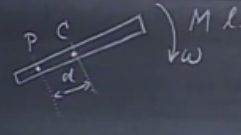
\includegraphics[scale=0.7]{\pIImages/lec21_rod}
\end{center}

The moment of inertia for rotation about the center of axis of a rod of uniform density is $\displaystyle \frac{1}{12} M \ell^2$, so angular momentum relative to point P is

\begin{equation}
|L_P| = I_P \omega = \left(\frac{1}{12} M \ell^2 + M d^2\right) \omega
\end{equation}

where the $M d^2$ term is added because of the parallel axis theorem.

There will be a force acting on the ruler at point P, as well as one acting on the pin (that it rotates around) \emph{by} the ruler. We can show this by analogy. Consider a massless rod, with two equal masses on each end. We rotate this rod about the center of mass, which is also the center of the rod. There is a centripetal force inwards on each of the masses, of equal magnitude since the masses are equal and the distance from the point of rotation are equal (and the velocities of the masses are then also equal).\\
However, if we rotate the rod about a point that is closer to one of the masses, then the centripetal force on that mass is smaller, but the centripetal force no the other is larger, since they move in circles of different radius. (As the point of rotations comes closer to one of the masses, it almost doesn't rotate at all, but rather spins about its axis.)

For this reason, there will be a force on the pin (and a reaction force from it) at point P in the ruler. The \emph{torque} relative to point P is zero, however: the force is along the ruler, and the position vector in $\vec{r} \times \vec{F}$ is also along the ruler.

Since $|\vec{\tau_P}| = 0$, angular momentum is conserved in this case. It would not be if we chose any other \emph{stationary} point, however.

Let's now rotate the same ruler about the center of mass C. The problem is now symmetric, like the case with the two masses mentioned above, and so there is now no net force on the pin/due to the pin. With no net force, $\vec{\tau_Q} = \vec{r_Q} \times \vec{F}$ must be zero for \emph{all} points Q, since $F = 0$. Therefore, in this case, angular momentum is conserved relative to \emph{all} points, as there is no net torque relative to \emph{any} point. The magnitude of the angular momentum for the rotation about the center of mass is then simply $I_C \omega$, which for a rod is

\begin{equation}
|L_{CM}| = \frac{1}{2} M \ell^2 \omega
\end{equation}

for all points in space.

\subsection{Off-center impulse: translation and rotation}

Let's now consider a ruler, lying flat on a frictionless table. It has a uniform mass density, and so its center of mass C is located at the geometric center. We give it an impulse $I$, in other words, a force that acts for a certain amount of time (a very short amount of time in this case, but that is not strictly necessary for this to hold).

\begin{center}
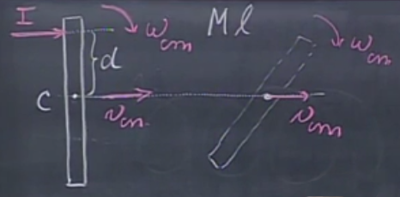
\includegraphics[scale=0.7]{\pIImages/lec21_ruler_rotation}
\end{center}

What will happen? Clearly, it is going to move towards the right. It will also rotate, assuming you don't aim for the center of mass (i.e. assuming $d \neq 0$).

The object \emph{must} rotate about its center of mass -- anything else is impossible. If it were to rotate about a point offset from the center of mass, then the center of mass would have to move in a spiral-ish motion. Due to conservation of (linear) momentum, the center of mass must have a constant velocity (meaning both magnitude and direction are constant!) after the initial push, which is only possible if any rotation is about the center of mass.\\
(Keep in mind that this is assuming a frictionless table. On a real table, where $\mu$ likely differs at different points, the results may also therefore differ: there is then an external force that may vary in unpredictable ways!)

That much is fairly intuitive, in my opinion, but what's interesting that the distance $d$ from the center of mass where the impulse happens does not affect the velocity of the center of mass. For a given amount of momentum given by the impulse, the velocity of the center of mass is constant, regardless of $d$. I find this nonintuitive, but it is still easy to see mathematically.

$\vec{p} = m \vec{v_{cm}}$ must hold, and since initial momentum is 0, $\vec{p} = \vec{I}$ after the initial push. Nowhere in the equation does $d$ appear -- the equation in question is valid for any isolated system, regardless of shape and place where the force is applied, as long as it is rigid.\\
Since $\vec{p} = \vec{I}$, the above equation also says that

\begin{equation}
\vec{v_{cm}} = \frac{\vec{I}}{m}
\end{equation}

$\omega$, on the other hand, clearly depends on the distance $d$. If $d = 0$, then $\omega = 0$; that much is clear. It is also clear that $\omega$ grows as $d$ grows. The reason is that the amount of torque (relative to the center of mass) provided depends on $d$ and the amount of force provided during the impulse. (The amount of angular impulse, i.e. change in angular momentum, depends on the average torque and the time, $J = \tau \Delta t$, just like how the linear impulse is given by $I = F \Delta t$.)\\
($\omega$ was calculated in this week's homework: week 9/homework 7, problem 9.)

However, note that if we instead look at the torque relative to a point P on the line of the impulse, i.e. a distance $d$ up from the center of mass, this torque is zero! Zero torque means angular momentum will be conserved, and so angular momentum \emph{relative to point P} is zero not only before, but also after the object starts to rotate. It is therefore conserved, unlike angular momentum relative to the center of mass!

\subsection{Physical pendulum}

Let's have a look at a different ruler. We previously derived an equation describing the motion of a simple pendulum, as a simple harmonic oscillator. We made some unrealistic approximations, however, including a massless string and a point mass hanging from it.\\
We will now consider a related yet different type of oscillator, called a physical pendulum.

In this case, we have a ruler, though the solution is valid for other shapes as well. We drill a hole through it at point P, and hang it on a small pin. The point P is located a distance $b$ from the center of mass, point C.

\begin{center}
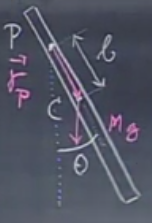
\includegraphics[scale=0.7]{\pIImages/lec21_physical_pendulum}
\end{center}

The ruler makes an angle $\theta$ with the vertical. Using the concept of the center of mass, we can consider gravity acting only at the center of mass; the magnitude is $M g$, where $M$ is the total mass of the ruler.

If we choose to use point P as our origin, our lives become much easier. There will be a force at point P, but if we choose it as our origin, we do not have to worry about those forces, since the torque due to those forces will be zero: $\vec{\tau_P} = \vec{0} \times \vec{F}$, since the first term is the position vector from P to P.

There is a torque that matters, relative to point P, however: the torque due to gravity acting on the center of mass. The distance $b$ acts as a lever arm, and the torque is given as the cross product between the distance and the force. The torque can also be found as $I_P \alpha$, as we saw earlier.

\begin{equation}
|\vec{\tau_P}| = \vec{b} \times \vec{F_g} = M g b \sin \theta = - I_P \alpha
\end{equation}

The torque is always trying to restore things back to equilibrium, which gives us a minus sign, just as how we used $- k x$ for the force when deriving the equation governing a spring oscillator. Note that we have used the Newton's second law equivalent for torques: $F = m a \Rightarrow \tau = I \alpha$.

$\alpha = \ddot{\theta}$ by definition, in a different form of notation. Now, using the small angle approximation that we have used several times earlier, $\sin \theta \approx \theta$. This is fairly valid for small angles; at 5 degrees, the difference is less than 0.15\%; at 10 degrees, the difference is about 0.5\%.\\
By using this approximation, and making the substitution for $\alpha$, we have

\begin{align}
M g b \theta &= - I_P \ddot{\theta}\\
I_P \ddot{\theta} + M g b \theta &= 0\\
\ddot{\theta} + \frac{M g b}{I_P} \theta &= 0
\end{align}

A-ha! This has the exact form of a simple harmonic oscillator! We already know the solutions; the square root of the stuff multiplying $\theta$ gives us the angular frequency $\omega$, etc:

\begin{align}
\theta(t) &= \theta_{max} \cos(\omega t + \phi)\\
\omega    &= \sqrt{\frac{M g b}{I_P}}\\
T         &= \frac{2 \pi}{\omega} = 2 \pi \sqrt{\frac{I_P}{M g b}}
\end{align}

Keep in mind that because $I_P \propto M$, this is in fact independent on the mass, just as with a simple pendulum. We can substitute in the value for $I_P$, in which case we transform the general result, above, into a result that only holds for a rod.\\
$I_P = \frac{1}{12} M \ell^2 + M b^2$ via the parallel axis theorem. Making that substitution,

\begin{align}
\omega    &= \sqrt{\frac{g b}{\frac{1}{12} \ell^2 + b^2}}\\
T         &= \frac{2 \pi}{\omega} = 2 \pi \sqrt{\frac{\frac{1}{12} \ell^2 + b^2}{g b}}
\end{align}

Again, note that these results are now only valid for the case of a rod.

As a side note, we can also write for the angular acceleration $\alpha = \dot{\omega}$. This is a very confusing thing to do, however! The omega in the previous sentence is the \emph{angular velocity}, i.e. how fast the angle is changing with time, analogous to the velocity $v$ for linear motion. This omega is \emph{constantly changing in time}, and has a minimum at $\theta_{max}$, as the pendulum reverses direction, and a maximum at $\theta = 0$.

On the other hand, the $\omega$ used in the cosine above, and the only one I have mentioned prior to the paragraph above to avoid confusion, is the \emph{angular frequency}, $\displaystyle \omega = \frac{2 \pi}{T}$. That $\omega$ is a \emph{constant}, and is only related to how many oscillations the pendulum completes per second. This sentence marks the last mention of the angular velocity $\omega$ in this section; only the one that represents angular \emph{frequency} will be used from here on.

Let's try to calculate the approximate period, including the uncertainty, of this pendulum when $\ell = 1.00$ m and $b = \SI{0.400(2)}{m}$, i.e. the uncertainty is 2 mm or 0.2 cm.

In the ideal case, the number we find by plugging in the numbers is $T = \SI{1.5497}{s}$, using $g = \SI{10}{m/s^2}$.\\
The largest possible time should be when $\ell$ and $b$ are both maximized, which gives $T = 1.556$ s. On the other side of things, the smallest possible period is about $T = 1.543$ s.

The uncertainty is about 0.0065 seconds or so; call it 0.01 s.\\
It turns out the professor used $g = \SI{9.8}{m/s^2}$, which is probably a good idea if you're going to time this in the real world. In either case, he found $T = 1.565$ seconds, which is very close to these numbers.

This is then demonstrated, and the timing indeed works out.

Next, we look at the same type of oscillation, but we use a hula hoop as the pendulum, instead of the ruler. The derivation is almost identical, and except for some variable names, we can still use the general equation we found earlier.

The center of mass of the hoop is at the geometric center, i.e. in the middle of empty space. We again hang it on a pin, at point P, which clearly is at the very top of the hoop.

\begin{center}
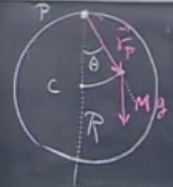
\includegraphics[scale=0.7]{\pIImages/lec21_hoop_pendulum}
\end{center}

As before, we consider the force of gravity as acting solely on the center of mass, with a force $M g$ downwards. Again as before, the position vector $\vec{r_P}$ acts as the lever arm, and the torque relative to point P is

\begin{equation}
\vec{r_P} \times \vec{F_g} = M g R \sin \theta = -I_P \ddot{\theta}
\end{equation}

As before, the torque must be equal to the negative of $I_P \alpha = I_P \ddot{\theta}$, using Newton's second law for circular motion. If we use the small angle approximation $\sin \theta \approx \theta$ again, and solve for $\ddot{\theta}$:

\begin{equation}
\ddot{\theta} + \frac{M g R}{I_P} \theta = 0
\end{equation}

Clearly, this is yet another simple harmonic oscillator! The only difference from the one we found for the rod is that we now used $R$ instead of $b$ for the distance to the center of mass; they are identical other than that non-detail.\\
The moment of inertia about point $I_P$ is the moment inertia about the center of mass $I_C$, plus $M R^2$ via the parallel axis theorem. $I_C$ is also $M R^2$ for a circular object with uniform mass distribution (all mass points are a distance $R$ away (derivation not shown), so $I_P = 2 M R^2$. That gives, using the solutions we found previously and using this new $I_P$,

\begin{align}
\theta(t) &= \theta_{max} \cos(\omega t + \phi)\\
\omega    &= \sqrt{\frac{g}{2 R}}\\
T         &= \frac{2 \pi}{\omega} = 2 \pi \sqrt{\frac{2 R}{g}}
\end{align}

This is the same result as we have found previously for a pendulum with a massless string, if we just call its length $2 R$! Quite neat, that they would have the same period.	

Time for an interesting lecture question.

\begin{center}
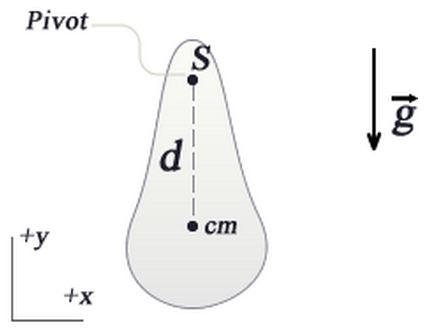
\includegraphics[scale=0.5]{\pIImages/lec21_physical_pendulum_2}
\end{center}

``A physical pendulum consists of a body of mass m contained in the xy-plane. The moment of inertia of the object about an axis perpendicular to the plane and passing through the object's center of mass is Icm.

The object oscillates in the xy-plane about the point S a distance $d$ from the center of mass as shown. What is the period of the pendulum for small angle oscillations where $\sin\theta \approx \theta$?''

Since they want the answer in terms of $I_{cm}$ (so that we don't need to actually calculate the moment of inertia) this should be fairly easy. In fact, we just use the general solution with $d$ as the distance between the point and the center of mass,

\begin{equation}
T = 2 \pi \sqrt{\frac{I_{S}}{m g d}}
\end{equation}

$I_S$ can be written as $I_{cm} + m d^2$, so

\begin{equation}
T = 2 \pi \sqrt{\frac{I_{cm} + m d^2}{m g d}} = 2 \pi \sqrt{\frac{I_{cm}}{m g d} + \frac{d}{g}}
\end{equation}

There is then a demonstration of the hula hoop, and a simple pendulum (an apple hanging on a lightweight string), to show that their periods are almost synchronized. (Most of the error likely comes from a small difference in length.)

%%% Local Variables:
%%% TeX-master: "../../main"
%%% End:


\section{Lecture 22: Kepler's laws, elliptical orbits, and change of orbits}

Let's begin with a quick review of circular orbits, before we move on to the more general (and more realistic) case of elliptical orbits.\\
In all the following equations, $m$ is the mass of the object that orbits (e.g. a satellite around the Earth, or the Earth itself around the Sun), while $M$ is the object at the center\footnote{For circular orbits; it is not at the center of elliptical orbits!} of the orbit. $G$ is the gravitational constant, and $R$ is the (fixed) distance between the two masses. $v$ is the orbital speed (tangential speed), and $T$ the orbital period. With all these variables in place, the following equations hold for circular orbits:

\begin{align}
T^2 &= \frac{4 \pi^2 R^3}{G M}\\
v &= \frac{2 \pi R}{T} = \sqrt{\frac{M G}{R}}\\
v_{esc} &= \sqrt{2}\ v = \sqrt{\frac{2 M G}{R}}\\
E_{total} = K + U &= \frac{1}{2} m v^2 - \frac{m M G}{R} = - \frac{m M G}{2R} = \frac{1}{2} U
\end{align}

Gravity is the only relevant force, and since gravity is conservative, mechanical energy is conserved. The total mechanical energy is, interestingly enough, always equal to half the gravitational potential energy, which makes it rather easy to find the total energy.\\
All bound orbits have negative total energy, as can be seen above (with $E_{total} = \frac{1}{2} U$, and $U < 0$ at non-infinite separations). If the total energy is zero, the orbit is unbound and parabolic (the object will never return; this is an escape trajectory), and if it is positive, it is hyperbolic (again, the object will never return).

We can find the orbital period by setting $\displaystyle \frac{m v^2}{R} = \frac{G M m}{R^2}$, where $\displaystyle v = \frac{2 \pi R}{T}$, and then solving for $T$.\\
The escape velocity can be found by setting $E_{tot} = 0$ and solving for $v$, since that causes an escape trajectory (as mentioned above).\\
The total energy is simply found by adding the kinetic energy at some point with the gravitational potential energy at that same point, and then substituting in $\displaystyle v = \sqrt{\frac{M G}{R}}$.

Let's now move on to elliptical orbits. Since a circle is a special case of an ellipse (with a semi-minor axis that equals the semi-major axis, or the eccentricity is 0, or the two foci coincide at the center; all of these must be the case for a circle), the above equations are good approximations for many orbits, since many orbits are very close to being circular (their eccentricity is very low).

In some cases, however, orbits can be extremely elongated; comets are a common example. Comet Hale-Bopp comes as close as 0.9 AU to the Sun, where 1 AU (astronomical unit) is the mean Earth-Sun distance, it then goes as far as 370 AU away. The eccentricity of the orbit is about 0.995, where $>1$ would mean a hyperbolic (unbound) orbit.

\subsection{Kepler's laws}

Kepler's first law states that planetary orbits are ellipses, where the Sun is located at one focus. Note that the Sun is then \emph{not} located at the center, except in the special case of a circular orbit, where both foci are are both located at the center.

Kepler's second law is best described with the help of an image.

%TODO: add image
%\begin{center}
%\includegraphics[scale=0.6]{\pIImages/lec22_keplers_2nd_law}
%\end{center}

Kepler's second law says that if the area $A_1$ is the same as the area $A_2$, the time taken to go between points 1 and 2 is the same as the time taken to go between points 3 and 4.

Kepler's third law says that $T^2 \propto \text{(mean distance)}^3$. This is often stated as $T^2 \propto a^3$, where $a$ is the semi-major axis or the orbit, which is equal to the mean distance in some ways of calculating the average, and not equal in other ways. The two statements are usually considered equivalent, however.

\subsection{Elliptical orbits}

Let's now consider the case of elliptical orbits.

\begin{figure}[H]
  \centering
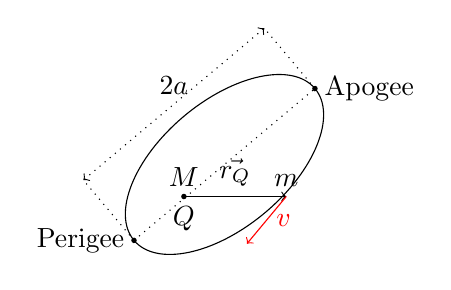
\begin{tikzpicture}
  \begin{scope}[rotate=40]
    \coordinate (P) at (1, 0);
    \coordinate (A) at (4, 0);
    \fill (P) circle (1pt) node[left] {Perigee};
    \fill (A) circle (1pt) node[right] {Apogee};
    \draw (2.5,0) ellipse (1.5 and 0.8);
    \draw[dotted] (P) -- (A);
    \draw[dotted] (P) -- (1, 1);
    \draw[dotted] (A) -- (4, 1);
    \draw[dotted, <->] (1,1) -- (4, 1) node[midway, above] {$2a$};
  \end{scope}

  \coordinate (M) at (1.4, 1.2);
  \coordinate (m) at (2.7, 1.2);
  \fill (M) circle (1pt) node[above] {$M$} node[below] {$Q$};
  \node[above] at (m) {$m$};
  \draw[->] (M) -- (m) node[midway, above] {$\vec{r_Q}$};
  \draw[red, ->] (m) -- (2.2, 0.6) node[midway, right] {$v$};
\end{tikzpicture}
\end{figure}

Say $M$ here represents the Earth, located an one focus of the ellipse. $m$ is perhaps a satellite or such that orbits the Earth, with velocity $\vec{v}$, with the position vector $\vec{r_Q}$ from Earth.\\
When the satellite is at the closest point to Earth, we say it is at \emph{perigee}. At the farthest point, it is at \emph{apogee}. The distance between apogee and perigee is $2a$, i.e. the major axis of the orbit.

If $M$ instead represented the Sun, and $m$ orbited the Sun instead (where $m$ could be the Earth, or some other planet), we instead call the closest approach \emph{perihelion}, and the farthest point is at \emph{aphelion}. The distance between the two extremes is still $2a$; only the names change.

We can now re-write a few of our equations:

\begin{align}
T^2 &= \frac{4 \pi^2 a^3}{G M}\\
v_{esc} &= \sqrt{\frac{2 M G}{r(t)}} \quad \text{(by setting $E_{tot} = 0$)}\\
E_{total} = K + U &= \frac{1}{2} m v(t)^2 - \frac{m M G}{r(t)} = - \frac{m M G}{2a} = \frac{1}{2} U
\end{align}

The total mechanical energy is still a constant (which is not proved here). Not only is it still constant, but it also has the same value as it would for a circular orbit with the same radius as the semi-major axis of the elliptical one. That is, all we do is replace the $R$ by $a$, and we have the constant energy total.

What is however not constant now is the two energy terms on their own. The kinetic energy now changes, since the orbital speed is no longer constant.\\
The gravitational potential energy also changes with time, since the distance to the Sun is no longer constant.

The escape velocity now also changes with time, though the expression looks about the same as it did for circular orbits, only that the constant radius $R$ has been replaced by the current distance to the sun, $r(t)$.

\begin{figure}[H]
  \centering
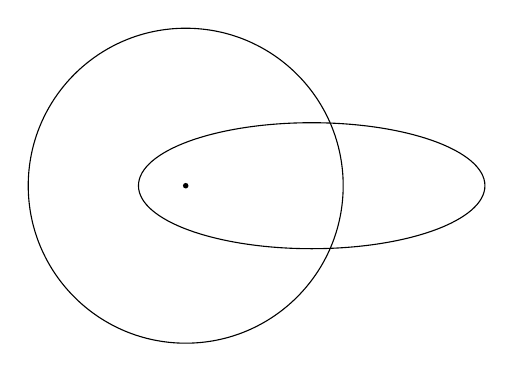
\begin{tikzpicture}
  \draw (1.6,0) ellipse (2.2 and 0.8);
  \draw (0,0) circle (20mm);
  \fill (0,0) circle (1pt);
\end{tikzpicture}
\end{figure}


These two orbits were drawn to have the same semi-major axis ($R = a$). This means that not only is the total mechanical energy the same for the two, but the time taken to complete one orbit is also exactly the same for either orbit.\\
What about angular momentum? Is it the same for both orbits, and if not, which one has more?

First off, angular momentum is conserved for elliptical orbits. This is clear if you use the same arguments as you do for circular orbits: the only relevant force is the gravitational force; that vector points straight from the planet towards the Sun. The position vector points straight from the Sun towards the planet. Therefore, the torque $\tau_Q = \vec{r_Q} \times \vec{F} = 0$, since the cross product of parallel/anti-parallel vectors is zero. With no external torque, angular momentum must be conserved -- \emph{with respect to the center of the orbit} Q, and not in general!

We can write the angular momentum relative to point $Q$ (the center of orbit) as $L_Q = \vec{r} \times \vec{p}$. However, in the case of the elliptical orbit, the magnitude of both these vectors change in time.  What doesn't change is the angular momentum relative to this point (see above). Because it is conserved, we can calculate the value at any point of the orbit, and if the value is smaller than it would be for a circular orbit of the same mean distance, that must mean the angular momentum is always smaller. (Or the other way around, if it is bigger.)

The answer is that it is smaller. Using the above information, consider a very elongated orbit, with a semi-major axis the same as the circular orbit we compare it to of course, but with a smaller semi-minor axis. Since angular momentum is constant, we can calculate the angular momentum at a point where it is very far from the Sun. Here, the position vector is large, but the velocity vector is small, and the angle between them is also small. This makes the cross product, proportional to the sine of the angle, small.\\
Alternatively, consider the case where the two orbits overlap. For the circular orbit, the position vector and velocity vector are always constant, and always at 90 degree angles.\\
In the case of the elliptical orbit, the position vector is the same, but the velocity vector differs, and makes a smaller angle with the position vector.

Let's now try to find some information about an orbit, given some initial conditions. We are have an object moving at a velocity $v_0$ near the Earth, which makes an angle $\varphi_0$ with the position vector $\vec{r_0}$ from the Earth, at some $t = 0$. Given these details plus the mass $M$ of the Earth, can we find all the details about the orbit, such as: the semi-major axis, the velocity at any given point, the perigee and apogee (closest and furthest distances from the Earth), and so on? The answer is yes, we can.\\

\begin{figure}[H]
  \centering
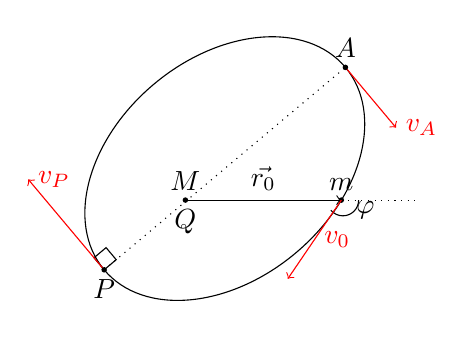
\begin{tikzpicture}
  \begin{scope}[rotate=40]
    \draw (0,0) ellipse (2.0 and 1.4);
    \draw[dotted] (-2,0) -- (2,0);
    \draw (-2,0) rectangle (-1.8,0.2);
    \draw[red, ->] (-2,0) -- (-2,1.5) node[right] {$v_P$};
    \draw[red, ->] (2,0) -- (2,-1) node[right] {$v_A$};
    \fill (-2,0) circle (1pt) node[below] {$P$};
    \fill (2,0) circle (1pt) node[above] {$A$};
  \end{scope}

  \fill (-0.5,-0.4) circle (1pt) node[above] {$M$} node[below] {$Q$};
  \fill (1.48,-0.4) circle (1pt) node[above] {$m$};
  \draw[dotted] (1.48,-0.4) -- (2.48,-0.4);
  \draw[->] (-0.5,-0.4) -- (1.48,-0.4) node[midway, above] {$\vec{r_0}$};
  \draw (1.7,-0.4) arc[start angle=0, end angle=-140, radius=0.2] node[right=2mm] {$\varphi$};
  \draw[red, ->] (1.48,-0.4) -- (0.8,-1.4) node[midway, right] {$v_0$};
\end{tikzpicture}
\end{figure}


We start out by finding the total mechanical energy, which we can use to find the semi-major axis. One of our equations for elliptical orbits is

\begin{equation}
E_{total} = K + U = \frac{1}{2} m v(t)^2 - \frac{m M G}{r(t)} = - \frac{m M G}{2a} = \frac{1}{2} U
\end{equation}

In this case, we can find the mechanical energy at this instant $t = 0$, since we know everything we need to know in the above equation:

\begin{align}
\frac{1}{2} m v_0^2 - \frac{m M G}{r_0} &= -\frac{m M G}{2a}\\
a \left(v_0^2 - \frac{2 M G}{r_0}\right) &= -M G\\
a &= -\frac{M G r_0}{v_0^2 r_0 - 2 M G}
\end{align}

Since $a$ cannot be negative, the second term in the denominator \emph{must} be greater than the first, so that the signs work out. We can rewrite the equation with this in mind:

\begin{equation}
a = \frac{M G r_0}{2 M G - v_0^2 r_0}
\end{equation}

This only holds for bound orbits. If $E_{tot} > 0$, $a$ must be negative, which makes no physical sense. The equation is simply invalid at in that case.

We can now apply
\begin{equation}
T^2 = \frac{4 \pi^2 a^3}{G M}
\end{equation}

given that we know $a$, so we also know the orbital period at this point.\\
The escape velocity also follows easily, since all you need to know there is $M$ and the distance to he center of that mass $r$.

Next up, we want to find the angular momentum of the orbiting object, relative to the center of the mass $M$ (which we call point Q), as the conservation of angular momentum is helpful for finding some other orbital properties. We can relate the initial angular momentum with the angular momentum at perigee (point P). The distance at perigee is QP, and so we have

\begin{equation}
|L_Q| = m v_0 r_0 \sin \varphi_0 = m v_p (QP)
\end{equation}
The first term is the cross product $(\vec{r_0} \times \vec {v_0}) m$, i.e. the angular momentum as we start out. The second term is the cross product $(\vec{r_p} \times \vec{v_p}) m$, only we call the distance QP instead of $r_p$.

Both $v_p$ and QP are unknown, so we need a second equation. We can find another using the conservation of mechanical energy. At point P, we have

\begin{equation}
\frac{1}{2} m v_p^2 - \frac{m M G}{QP} = - \frac{m M G}{2a}
\end{equation}

Now, as an added bonus, when we solve this, we will get two answers, since this equation is quadratic in $v_p$. One solution will be $v_p$, and the other will be $v_A$. We will also find both QP and QA (the perigee and apogee distances). The reason we find both of these values is rather simple: we have said that the angular momentum is $m v_p (QP)$. There are only two places where the position vector and the velocity vector are exactly perpendicular: at perigee, and at apogee. The equations are equally valid at both points, since the equation doesn't know that we said $v_p$ and QP; it might as well have said $v_A$ and QA, and we would have found the same answers.

The solutions I got were extremely ugly; I'm not sure if they can be simplified further using physics knowledge, but Mathematica can't do any better than this.

\begin{align}
v_p        &= \frac{a G M - \sqrt{a G M \left(a G M- r_0^2 v_0^2 \sin^2 (\varphi_0)\right)}}{a r_0 v_0 \sin (\varphi_0) }\\
\text{QP}  &= a + \sqrt{a\left(a - \frac{r_0^2 v_0^2 \sin^2(\varphi_0)}{G M}\right)}\\
v_A        &= \frac{a G M + \sqrt{a G M \left(a G M- r_0^2 v_0^2 \sin^2 (\varphi_0)\right)}}{a r_0 v_0 \sin (\varphi_0)}\\
\text{QA}  &= a - \frac{\sqrt{a G M(a G M - r_0^2 v_0^2 \sin^2(\varphi_0))}}{G M}
\end{align}

Because the angular momentum $m(\vec{r} \times \vec{v})$ must remain a constant at all times, it must be true that at perigee/apogee when the cross product equals simply $m r v$, the product of the distance and the velocity must be the same in both cases. That is, $m v_p (QP) = m v_A (QA)$. The mass cancels, of course, so we find that $v_p (QP) = v_A (QA)$ must hold.

Apogee is by definition farther from the Earth than perigee, so the speed at apogee must be lower.\\
The difference in speed can be rather enormous, for very elliptical orbits. If apogee is 14 times as far away as perigee is, the speed at perigee will then be 14 times \emph{higher} than the speed at apogee. If this were not the case, angular momentum would not be conserved (relative to the point Q, the only point relative to which it is \emph{ever} conserved).

So in conclusion, by knowing the initial position, velocity (including the direction, i.e. angle between position vector and velocity vector) and the mass of the object we orbit, we can find all the orbital details. This is assuming that the orbital will be elliptical ($a > 0$ when we calculate it, using the first equation). If that is not the case, then there will be no bound orbit, and some of these parameters are meaningless (such as apogee/aphelion, the orbital period, etc). In any case, we can not deal with that using what we have learned \emph{so far}.

\subsection{Change of orbits}

Let's look at a simplified case of a change in orbit. We begin in a fully circular orbit, and then fire a rocket exactly tangentially to the orbit.\\
Say we begin at the ``top'' of the orbit (in a diagram), at point X. We fire the rocket a very short amount of time, so that we can consider that it is still at X afterwards. The speed will increase, so the kinetic energy will increase, and the total mechanical energy will increase (we have not moved away, so gravitational potential energy must be the same, assuming our mass has not changed).

Because our velocity is now greater, and we are at a certain distance $R$ from the planet (or star, or whatever), our velocity is no longer the correct velocity for a circular orbit at this distance. Instead, we go into an elliptical orbit, where $a > R$. The total mechanical energy has increased, which means $a$ must increase; total mechanical energy is $-\frac{m M G}{2 a}$, and for mechanical energy to increase, that number must become less negative. A larger $a$ does exactly that. Via the relationship in $T^2$, this also implies that the period of this new orbit is greater than the old period, despite the increase in speed.

\begin{figure}[H]
  \centering
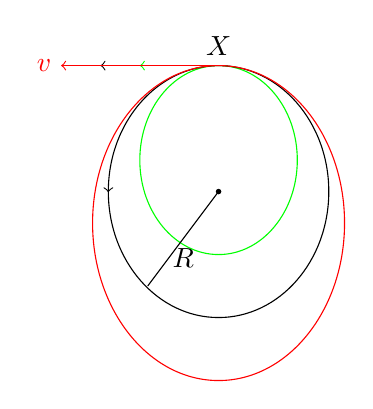
\begin{tikzpicture}
    \draw[green] (0,-1.2) ellipse (1.0 and 1.2);
    \draw[green, ->] (0,0) -- (-1,0);
    \draw (0,-1.6) ellipse (1.4 and 1.6);
    \draw[->] (0,0) -- (-1.5,0);
    \draw[red] (0,-2.0) ellipse (1.6 and 2.0);
    \draw[red, ->] (0,0) -- (-2,0) node[left] {$v$};
    \node[above] at (0,0) {$X$};
    \fill (0,-1.6) circle (1pt);
    \draw (0,-1.6) -- (-0.9,-2.8) node[midway, below] {$R$};
    \draw[->] (-1.4,-1.6) -- (-1.4,-1.61);
\end{tikzpicture}
\end{figure}

In this graphic, the original orbit (fully circular) is in white. We are orbiting counterclockwise, as seen here.\\
For the red orbit, we have increased our tangential velocity, and so the orbit grows, and becomes elliptical. $E_{tot} > E_{tot,circular}$, and so the semi-major axis is greater than the original radius, and the period is greater than the original, since $T^2 \propto a^3$.

For the green orbit, we instead fired our rocket exactly opposite to our velocity, so that we slowed down, and lost kinetic energy, and also lost total mechanical energy.\\
In that case, $a < R$, and the period goes down.\\
Out of context, it sounds rather crazy: you go around faster by braking! Of course, you also travel a shorter distance per period, so there's nothing particularly crazy about it.

The rest of this lecture will focus on a ``practical'' (fun, at least) example of this; perhaps we can call it several examples, even.

Two astronauts, Peter and Mary, are in orbit around the Earth. They are both moving at the same speed, and are at the same distance from Earth, sharing a circular orbit. They are not moving along it together, however. Peter is at one place along this circular orbit, point X, while Mary is at a point M, a distance further along. We can specify this separation as a fraction of the circumference $2 \pi R$ of the orbit, using $f$ as the fraction. The distance between the two is then $f\ 2 \pi R$. The rest of the orbit must then be $(1-f) 2 \pi R$, which is the amount of distance Mary must move before she ends up at point X (which she recently passed).

\begin{figure}[H]
  \centering
\begin{tikzpicture}
    \draw[*-*] (0,1.5) arc[start angle=90, end angle=160, radius=15mm] node[at start, above] {$PX$} node[at end, left=1mm] {$M$};
    \draw[->] (0,1.5) arc[start angle=90, end angle=200, radius=15mm];
    \draw[green, thick] (0,0) circle (15mm);
    \draw[red, thick] (0,1.5) arc[start angle=90, end angle=160, radius=15mm] node[midway, left] {$F2\pi R$};
\end{tikzpicture}
\end{figure}



Say the radius of this shared orbit is $R = 7000$ km ($\SI{7e6}{m}$), and $f = 0.05$, which makes the separation between the two about 2200 km. (The actual separation as a straight line is smaller, but we don't really care about that.)\\
Given these parameters, there is a only one possible circular orbit: the radius of the orbit puts a demand on the velocity and period of the orbit. This velocity is about 7.55 km/s, and the period is about 97 minutes.

If we round things off a bit, it then takes $f T \approx 5$ minutes to travel the distance that exists between Peter and Mary. This means it takes 92 minutes for Mary to get to the point where Peter is currently. (Needless to say, Peter will no longer be there when she gets there.)

Now, here is the problem: Mary forgot her lunch. She radius Peter, who says not to worry; he will throw her a ham sandwich. The question is: how will he do this, so that Mary can catch it? Perhaps the simplest way is to throw the sandwich such that its new orbit brings it to point X, where Mary will be, in exactly the 92 minutes required, so that Mary and the sandwich meets at that point.

Here comes the counter-intuitive part (at least to me): if Peter throws the sandwich forward, it will come back to point X \emph{later} than Mary. The faster he throws it, the longer it will take.\\
The reason is that by throwing it, he is doing exactly what we did with the rocket earlier on. The sandwich will move into an elliptical orbit, with $a > R$. Since $T \propto a^{3/2}$, this orbit has a longer period than Peter's, and so the sandwich will take a longer time to get into place for Mary's move past point X.

Instead, he needs to throw it \emph{backwards}, and \emph{reduce} its orbital speed. That way, it will move into a smaller orbit, with a smaller period, and come back to point X faster, by having moved a smaller distance.

What we need is that the orbital period of the sandwich $T_s$ is less than Mary's period $T_a$ (a for astronaut), such that $T_s = (1 - f) T_a$. $T_a$ is 97 minutes, and the orbit we want should be 92 minutes. $1 - f = 0.95$, and $0.95 \times 97$ minutes is about 92 minutes. (Keep in mind that all of these numbers for the period are rounded approximations; the actual period $T_s$ will be exactly right.)

Doing the actual math, we need the sandwich's orbit to be $(1-f)$ times the astronauts' orbit, as mentioned, which using Kepler's third law is

\begin{equation}
\sqrt{\frac{4 \pi^2 a^3}{G M}} = (1-f) \sqrt{\frac{4 \pi^2 R^3}{G M}}
\end{equation}
\begin{align}
\sqrt{a^3} &= (1-f) \sqrt{R^3}\\
a &= (1-f)^{2/3} R
\end{align}

So knowing only the radius of their orbit and how far they are apart along that orbit (as measured by a fraction $f$ of the total circumference), we can find what the radius of the sandwich, $a$, must be.\\
Knowing $a$, the semi-major axis of the sandwich's orbit, we can now calculate what velocity it must have, using the equation for total mechanical energy.

\begin{equation}
\frac{1}{2} m v_s^2 - \frac{m M G}{R} = -\frac{m M G}{2a}
\end{equation}

On the right-hand side, we have the current kinetic energy of the sandwich (after the throw), and its current gravitation potential energy. An instant after the throw, we can still consider it to be at point X, so it is still a distance $R$ from the planet. The right-hand side of the equation must always hold for elliptical (and thus also circular) orbits: the total mechanical energy is always $\displaystyle \frac{1}{2} U$.

We can solve this for $v_s$, now that we know everything else. $m$ cancels, as always, and in the end, we find

\begin{align}
\frac{1}{2} v_s^2 - \frac{2 M G}{R} = -\frac{M G}{a}\\
v_s^2 = \frac{2 M G}{R} - \frac{M G}{a}\\
v_s^2 = \frac{2 M G}{R} - \frac{M G}{a}\\
v_s = \sqrt{\frac{G M (2 a - R)}{a R}}
\end{align}

In terms of $R$ (since we know $a$), this is also

\begin{equation}
v_s = \frac{\sqrt{(2(1-f)^{2/3} - 1) G M R}}{(1 - f)^{1/3} R}
\end{equation}

In terms of numbers, we have $a = 6765$ km -- smaller than $R$, which it must be; $v_s = 7.42$ (though closer to 7.43) km/s.\\
The speed of the sandwich \emph{relative to Peter} is what matters to hit, though: he doesn't need to throw it at over 7 km/s! He just needs to throw it so that its final velocity $v_s$ is that value, but most will come from his current orbital speed $v_a$.

The speed he needs to throw it at is $v_s - v_a = 0.13$ km/s. Note how $v_s < v_a$ -- it moves in a smaller orbit, but therefore also moves at a lower speed.

So in order for Mary to catch it the \emph{first time she passes point X again}, he must throw the sandwich \emph{backwards} (towards the clockwise direction), slowing its speed and reducing its total energy, even though he can see Mary currently in front of him!

Unfortunately, 130 m/s is a bit much for a person to throw a sandwich. We can find a different solution, where the sandwich moves around the Earth multiple times, and possibly where Mary does too.\\
Mathematically, we can have Mary pass the point $n_a$ times ($n$ for number of times, $a$ for astronaut), and the sandwich $n_s$ times. Both numbers need to be integers, of course.

We now find

\begin{equation}
a = R \left(\frac{n_a - f}{n_s}\right)^{2/3}
\end{equation}

as the semi-major axis for the sandwich's orbit. If $n_a = n_s = 1$, the equation reduces down to what we had previously.\\
Not all combinations of integers will work, however.

For $n_a = 1$ and $n_s = 3$, such that the sandwich should make three orbits in the same time Mary completes her one orbit, the result is invalid.\\
For these numbers, we find $a = 3252$ km (versus $R = 7000$ km).\\
$2a < R$, which is not allowed; the reason why can be seen in the equation for $v_s$. If we the $a$ value in, we find an imaginary answer (complex, but the real part is 0).\\
As $a$ approaches $R/2$, $v_s$ goes to zero. There is the possibility where he throws it at exactly his orbital speed, in which case it will stand still relative to the Earth, and fall straight down. What if he throws it ever faster? In that case, there is clearly no longer a counterclockwise orbit, which has been our assumption all along.

The final part of the lecture shows a computer simulation of this scenario, including a few cases not mentioned in this text.

\section{Lecture 23: Doppler effect, binary stars, neutron stars and black holes}

The speed of sound, in air, is about 340 m/s, at roughly room temperature. The range is something like 306 m/s near $-40$ degrees Celcius (which also equals $-40$ degrees Fahrenheit) and 360 m/s at 50 degrees Celcius ($122^\circ$ F), which hopefully covers most temperatures we encounter.

When a person speaks, his/her vocal cords oscillate at a certain frequency, which causes a pressure wave in the air to move towards you, at the speed of sound. Your eardrums then oscillate at the this same frequency, which your brain can interpret as a certain pitch.

If the sound transmitter is moving away or towards the receiver, the perceived sound frequency will change. The faster the transmitter is approaching you, the higher the perceived frequency, and vice versa. If the transmitter is moving away from you at the speed of sound, you will hear exactly half the original frequency.\\
That is, if we use prime notation for the perceived frequency and $f$ for the original frequency,

\begin{align}
f' &> f \text{ (when sound source is approaching you)}\\
f' &< f \text{ (when sound source is moving away from you)}
\end{align}

More quantitatively, when a source source is moving towards you, but you are sitting still, the frequency you perceive is

\begin{equation}
f' = f(1 + \frac{v}{v_s} \cos \theta)
\end{equation}

where $v_s$ is the speed of sound, and $v \cos \theta$ is the radial speed, i.e. the speed at which the transmitter is moving towards you. If the transmitter is moving quickly, but at a 90 degree angle to you, you don't hear any shift in the frequency.\\
If the transmitter is moving \emph{away} from you, the frequency you perceive goes down, which this equation also captures (for negative values of $\cos \theta$).

The professor demonstrates this by using a 4000 Hz tuning fork, moving it back and forth towards and away from the students. If this is done at roughly 1 m/s, the pitch will change with $\pm 0.3$\% which is $\pm 12$ Hz. This difference is clearly audible, including in the recorded video of this lecture.

This effect of frequency change is known as the \emph{Doppler effect}. It is the reason behind the familiar scenario where the pitch of an ambulance/police car/fire truck's siren changes as it travels past you.\\
When the sound transmitter is moving away from you, the pitch you hear is lower than the pitch that is actually transmitted at the source. If the transmitter is coming towards you, the pitch instead increases.

Note that the case of a stationary transmitter and a receiver moving away is \emph{not} equal to the case of a stationary receiver where the transmitter is moving away!

If the transmitter is stationary, and is creating sound waves with a frequency of say 440 Hz (the standard tuning in all modern music is to the A440 note), and the receiver moves away at the speed of sound, then there will be no sound heard at all - the receiver (just barely) outruns the sound waves entirely!

On the other hand, if the \emph{transmitter} is moving away at the speed of sound, while the receiver is stationary, the result is that the perceived frequency is cut in half to 220 Hz.\\
So we still hear the sound, in this case. If you find that nonintuitive, think about it a bit more - it's very clear that while the transmitter moves, the waves will still reach you as they always travel at 340 m/s in your direction. The transmitter may be moving in a direction away from you, but the sound waves don't travel along with the transmitter, but towards you (and it all other directions, too, assuming an omnidirectional speaker).

Let's now consider the case where the transmitter is moving around in a circle. Now, the perceived frequency, assuming the receiver is still stationary, will vary sinusoidally around the base frequency of $f$ that the transmitter is sending out.

\begin{figure}[H]
  \centering
  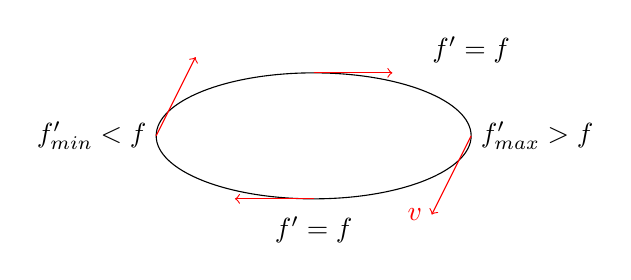
\begin{tikzpicture}
    \draw (0,0) ellipse (2 and 0.8);
    \draw[red, ->] (0, 0.8) -- (1, 0.8);
    \draw[red, ->] (0, -0.8) -- (-1, -0.8);
    \draw[red, ->] (2, 0) -- (1.5, -1) node[left] {$v$};;
    \draw[red, ->] (-2, 0) -- (-1.5, 1);

    \node at (2,0) [right] {$f'_{max}>f$};
    \node at (-2,0) [left] {$f'_{min}<f$};
    \node at (2,0.8) [above] {$f'=f$};
    \node at (0,-0.8) [below=1mm] {$f'=f$};
  \end{tikzpicture}
\end{figure}
  

When the source is moving straight towards you, $f'$ is at a maximum; the opposite is true when it is moving straight away from you. At the other two extremes, when it is at 90 degree angles, $f' = f$, and so there is no change in frequency at those times. In between, as you might expect, there is a gradual change between these extremes.

If we, as the receiver, plotted the frequency we heard as a function of time, we would get something like this:

\begin{figure}[H]
  \centering
  \begin{tikzpicture}
    \draw (0,1) cos (1,0) sin (2,-1) cos (3,0) sin (4, 1) cos (5,0) sin (6,-1) cos (7,0) sin (8, 1) cos (9,0);

    \draw[dotted] (0,0) -- (10,0);
    \draw (-1,-2) -- (10,-2);
    \draw (0,-3) -- (0,2.5);

    \fill (0,0) circle (2pt) node[left=1mm] {$f$};
    \draw[thick] (-0.2,1) -- (0.2,1) node[left=1mm] {$f'_{max}$};
    \draw[thick] (-0.2,-1) -- (0.2,-1) node[left=1mm] {$f'_{min}$};
    \draw[dotted] (0,-1) -- (2,-1);

    \draw[->] (8,-2.5) -- (9,-2.5) node[right] {$t$};

  \end{tikzpicture}
\end{figure}
 


If we have this curve, we can calculate an impressive number of things. First, we know ${f'}_{max}$ and $f$, which means we can calculate the velocity of the transmitter.\\
We can also measure the period of one rotation, by measuring the time from one peak to the next (or one valley to the next, etc). Knowing that, we can find the radius $R$ of the circle the transmitter is moving in:

\begin{align}
\frac{2 \pi R}{T} = v_{tr}\\
R = \frac{T v_{tr}}{2 \pi}
\end{align}

So from simply listening to/measuring the sound over time, we can calculate these three things, rather easily.

% Doppler ilustration
% Taken from https://tikz.net/wave_doppler/
\begin{figure}[H]
  \centering
\begin{tikzpicture}
  [
    pics/eye/.style={
      code={
        \draw (#1-180:0.5) to[out=#1,in=#1-240,looseness=0.9] (#1-90:0.25)
              (#1-180:0.5) to[out=#1,in=#1-130,looseness=0.9] (#1-270:0.25);
        \clip (#1-180:0.47) to[out=#1,in=#1-240,looseness=0.9] (#1-90:0.24) --
              (#1-270:0.242) to[out=#1-130,in=#1,looseness=0.9] cycle;
        \draw[very thin,top color=white,bottom color=red!60!black!20,shading angle=#1-120]
           (#1-180:0.48) circle(0.45);
        \fill[brown!30!black,rotate=#1-180]
          (0.07,0) ellipse({0.05} and 0.12);
        \fill[black,rotate=#1-180]
          (0.05,0) ellipse({0.03} and 0.06);
      }},
    pics/eye/.default=180
  ]
  \def\R{1.5}      % radius
  \def\N{5}        % number of wave fronts
  \def\lam{\R/\N}  % wavelength
  \def\angmin{30}  % min. angle velocity arrow
  \def\angmax{330} % min. angle velocity arrow
  \def\waves#1{
    \foreach \i in {1,...,\N}{
      \draw[myblue,thick] ({-(\i-0.25)*#1*\lam},0) circle ({\lam*(\i-0.25)});
    }
    \foreach \a in {\angmin,90,150,210,270,\angmax}{
      \draw[-{Latex[length=3,width=2]},vcol] ({-(\N-0.25)*#1*\lam},0)++(\a:\R-0.50*\lam) --++ (\a:\lam);
    }
    \fill[myred] (0,0) circle (0.06);
  }
  \def\s{0.61}
  \draw[myblue!20,dashed,very thin,dash pattern=on 1 off 1]
    ({-(\N-0.25)*\s*\lam},0) -- (0,0);
  \fill[myred!20] ({-(\N-0.25)*\s*\lam},0) circle (0.06);
  \waves{\s}
  \node[vcol] at (30:{1.15*\R-\s*\R} and 1.2*\R) {$c$};
  \draw[{Latex[length=3,width=2]}-{Latex[length=3,width=2]}]
    (-0.9*\R-\s*\R,-0.8*\R) node[left=-1,scale=0.7] {$y$}
    |-++ (0.15*\R,-0.15*\R) node[right=-1,scale=0.7] {$x$};
  %\draw[dashed] (\R-\s*\R,0) --++ (0,-1.3*\R);
  %\draw[dashed] (0,0) --++ (0,-1.3*\R);
  %\draw[dashed] (-\R-\s*\R,0) --++ (0,-1.3*\R);
  \pic at ( 1.25*\R-\s*\R,0) {eye={180}};
  \pic at (-1.15*\R-\s*\R,0) {eye={0}};
  \draw[-{Latex[length=4.8,width=3.8]},white,line width=1.2]
    (0.05,0) -- (0.22*\R+0.02,0);
  \fill[myred] (0,0) circle (0.06);
  \draw[-{Latex[length=4,width=3]},thick,vcol,line cap=round]
    (0.05,0) -- (0.22*\R,0); %node[right=-1] {$v$};
  \begin{scope}[shift={(0,-1.35*\R)}]
    \draw[myblue,thick,samples=100,smooth,variable=\x]
      plot[domain=-(\s+1)*(\R):0](\x,{0.1*\R*sin(360/(\s+1)/(\lam)*\x)}) %--
      plot[domain=0:(1-\s)*(\R)](\x,{-0.1*\R*sin(360/(1-\s)/(\lam)*\x)});
    \fill[myred] (0,0) circle (0.05);
    \draw[-{Latex[length=3,width=2]},vcol] ({-(\s+1)*(\R-0.25*\lam)},0.04*\R) --++ (-\lam,0);
    \draw[-{Latex[length=3,width=2]},vcol] ({(1-\s)*(\R-0.25*\lam)},0.04*\R) --++ (\lam,0);
    \draw[{Latex[length=3,width=2]}-{Latex[length=3,width=2]}]
      (-\R-\s*\R-2.3*\lam,0.06*\R) node[left=-1,scale=0.7] {$z$}
      |-++ (0.15*\R,-0.15*\R) node[right=-1,scale=0.7] {$x$};
  \end{scope}
  %\draw[<->] (0,-1.5*\R) --++ (\R-\s*\R,0)
  %  node[midway,right=2,below=1,scale=0.6] {$\sim c-v$}; %{$\sim\dfrac{c}{c+v}$};
  %\draw[<->] (0,-1.5*\R) --++ (-\R-\s*\R,0)
  %  node[midway,below=1,scale=0.6] {$\sim c+v$}; %{$\sim\dfrac{c}{c-v}$};
\end{tikzpicture}
\end{figure}


\subsection{The Doppler effect and electromagnetic waves/light}

Let's look more at the Doppler effect in light (and other EM radiation).

\begin{figure}[H]
  \centering
  \begin{tikzpicture}

    \draw[*-*] (0,0) -- (5,0) node[right] {$f'$};
    \node at (0,0) [left] {$tr_f$};
    \draw[red, ->] (0,0) -- (2,1) node[right] {$v_{tr}$};
    \draw[red, ->] (0,0) -- (2,0) node[below] {$v\cos{\theta}$};

    \draw (1,0.5) arc[start angle=40, end angle=-10, radius=0.6] node[midway, right] {$\theta$};
  \end{tikzpicture}
\end{figure}
 

The equation given in lecture, which is only valid for $v \ll c$, i.e. when the relative velocity between transmitter and receiver is much smaller than the speed of light, is:

\begin{equation}
f' = f (1 + \frac{v}{c} \cos \theta)
\end{equation}

In calculating the Doppler shift due to some relative motion, only the radial component, meaning the part of the velocity that is directly towards or from you, matters. Therefore, we take the cosine of the angle of the velocity vector. Note that the radial component is given as $v \cos \theta$, rather than $v_{tr} \cos \theta$ (tr for transmitter); the index was dropped as it does not matter whether the transmitter or the receiver is moving, or both. (It is even really a meaningless question in relativity; moving relative to what reference frame?)\\
There is however something known as the transverse Doppler shift, which occurs even at 90 degree angle. I'm not sure when this matters, but it is not mentioned in the lecture, at all, so I suppose it is less important in most cases.

Much of the idea behind special relativity, as the name implies, is that motion is relative. There is no such thing as an absolute reference frame, and therefore, there is only one term of velocity in the equation. It is meaningless to ask whether person A is moving towards person B, or person B is moving towards person A. What we can say is that they are approaching each other.\\
It does however, of course, matter whether the two are approaching or receding from each other.

In this equation, if $\theta < \ang{90}$, $f' > f$ since the cosine term will contribute to increasing $f'$. If $\theta > \ang{90}$, the cosine will be negative, and $f' < f$. At 90 degree angles, as mentioned, this equation will tell you that there is zero Doppler shift. And again, this only holds if $v \ll c$, i.e. $\displaystyle \frac{v}{c} \ll 1$.

All electromagnetic radiation, whether it is visible light, gamma rays, microwaves, radio waves etc., has a frequency associated with it. Anything with a frequency of oscillation also has a \emph{period} of oscillation, with the simple relationship that $T = 1/f$.\\
How far does EM radiation travel in a time T? Well, it travels at the velocity $c$, the speed of light ($c \approx \SI{3e8}{m/s}$, to within 0.07\%). That means the distance traveled is $\lambda = c T$, where $\lambda$ (lowercase Greek letter lambda) is the symbol we use to denote \emph{wavelength}.

\begin{equation}
\lambda = c T = \frac{c}{f}
\end{equation}

For example, if $T = \SI{2e-15}{s}$, $\lambda = \SI{6e7}{m}$, which is the about wavelength of red light.\\
If instead $T = \SI{1.3e-15}{s}$, $\lambda = \SI{3.9e7}{m}$, which we perceive as blue light.

In optical astronomy, we can only measure the wavelength of light -- not frequency or period -- so we can rewrite some of our equations to better accommodate this. We can of course calculate frequency, so that

\begin{align}
f  &= \frac{c}{\lambda}\\
f' &= \frac{c}{\lambda'}
\end{align}

With that in mind, we can find

\begin{equation}
\lambda' = \lambda(1 - \frac{v}{c} \cos \theta)
\end{equation}

What was a plus sign in the previous equation of this sort is now a minus sign. Also, keep in mind that this equation also has the restriction that $v \ll c$.

Since frequency is inversely proportional to wavelength, $\lambda' < \lambda$ if the object is approaching you ($\theta < \ang{90}$). This is known as \emph{blueshift}. The name comes from the fact that all radiation becomes more energetic (higher frequency/smaller wavelength), which causes visible light to shift towards the blue end of the spectrum. (EM radiation that is already more energetic than blue/violet light becomes even more energetic, and therefore shifts even further away from the visible spectrum, towards the gamma rays.)

Similarly, if the object is moving away from you, $\theta > \ang{90}$ and $\lambda' > \lambda$. A longer wavelength means less energy, and this is known as \emph{redshift}. Here, all light becomes less energetic and ``stretched out'', which shifts visible light (and all more energetic light) towards the red end of the spectrum. Light that was already lower energy (microwaves, radio waves) lose further energy and shift further away from the red (and further from visible light altogether).

In case the above is written in a confusing manner: blueshift is called as such because visible light is shifted towards the blue. \emph{All} light, regardless of frequency/wavelength becomes \emph{more} energetic when blueshifted. Conversely, redshift is called as such because visible light is shifted towards the red, and all light, regardless of frequency/wavelength becomes \emph{less} energetic when redshifted.

\subsection{Emission and absorption spectra}

We can look at the light spectra of stars, and look at the intensity of the light as a function of wavelength. When plotting that, we will not see a continuous distribution, as we might expect. Instead, we see a mostly smooth curve, with some sharp spikes downwards. That is, light intensity is sharply reduced for certain wavelengths.\\
We call these \emph{absorption lines}. Each absorption line is due to some element present in the atmosphere of the star. Through the process of figuring out which elements and isotopes cause which absorption lines here on Earth, we can use the lines to figure out which elements are present in the star.


%TODO: add images
%Here is an example of \emph{emission lines}, in this case of hydrogen:
%\begin{center}
%\includegraphics[scale=0.75]{\pIImages/lec23_hydrogen_emission}
%\end{center}

The red line on the right is known as H$\alpha$ (hydrogen alpha), and is a very well-known spectral line. Telescopes are often fitted with H$\alpha$ filters for viewing the Sun.\\
Emission lines are the \emph{opposite} of absorption lines. In this case, we use a lamp or such that excites hydrogen, which then only produces light in discrete steps, for quantum mechanical reasons.

If you have ever seen street lightning that makes everything appear yellow, those lamps were most likely sodium-vapor lamps. These lamps, especially the low-pressure type, are almost entirely monochromatic, and essentially only emit light at two wavelengths, about 589.0 and 589.6 nm -- both of which are yellow.\\
Since vision relies on having light reflect off things and enter our eyes, in the presence of only such light, it is impossible to see colors other than yellow. Objects that completely absorb yellow will become dark. For this reason, the amount of different wavelengths a lamp emits is a common measure of its perceived quality (see color rendering index aka color rendition index, CRI).

As mentioned, absorption lines are the opposite of this. Here is an example of absorption lines:

%TODO: add images
%\begin{center}
%\includegraphics[scale=0.75]{\pIImages/lec23_absorption_spectrum}
%\end{center}

The letters refer to labels of Fraunhofer lines, a set of spectral lines named after (and identified by) German physicist Joseph van Fraunhofer, in the early 1800s. The sodium lines above can be seen as D1 and D2 in the yellow-orangeish part of the spectrum.

The now-well known element helium was first discovered in Sun, as an absorption line that could not be reproduced in the lab here on the Earth was identified. The element was named  helium, after Helios, the Greek Sun god.

What is now interesting, and extremely useful, is that the relative spacing of these lines stays constant. If a star is moving (radially) relative to us, the light will be either redshifted (if it moves away) or blueshifted (if it moves towards us), but since \emph{the entire spectrum} will be shifted, we can still identify what elements are present via their distinct patterns and spacings.\\
This means that we can not only look at a star and figure out what it is made of, we can also calculate its velocity relative to us!

For example, if $\lambda'/\lambda = 1.000333$, according to the equation we found earlier, the star is moving at $-0.000333 c$ (radially), where the minus sign signifies that it moves away from us. That is, $v \cos \theta = -0.000333c = -100$ km/second. Note that since $\lambda' > \lambda$, the light from the object has been redshifted. Also note that we cannot say what $v$ is using this information, only what the radial component is -- i.e. how fast it moves towards us, or from us.

As a very quick aside, this is how police ``radar guns'', which can measure the speed of cars, work. They reflect radar waves of a known frequency/wavelength off cars, and measure the wavelength of the returning waves. The radial velocity of the car can then be calculated, using the measured Doppler shift.

\subsubsection{Spectra of binary stars}

Binary stars, pairs or stars that orbit each other, are extremely common. The lecture states that half of the stars in the sky are binaries. I'm not sure if that refers to visible stars, in which case I would guess nothing has changed, but it \emph{may} (with emphasis, indeed) be that science's view has shifted, and that most stars overall are in fact not binaries, from recent (post-lecture recording) news articles.

When binary stars orbit each other (or rather their shared center of mass), we can measure the Doppler shift they exhibit. While orbiting, they will be going towards us, at right angles, from us, etc. just as with the sound source moving in a circle we looked at earlier.\\
This is only possible to see if we are in the plane of their orbit, however. If we are looking at the system from ``above'', the radial component of the velocity between the stars and us will be constant despite the orbit, as they will not move any closer to us or further from us due to the orbit.

Just as in the case with sound, we can measure and calculate the period of this shift, and therefore calculate their velocities, the orbital period, and the orbital speed.

%TODO: 
%\begin{center}
%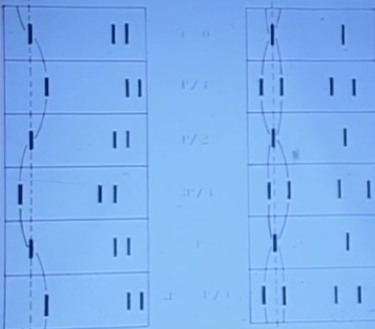
\includegraphics[scale=0.75]{\pIImages/lec23_binary_spectrum}
%\end{center}
%\begin{figure}[H]
%\begin{tikzpicture}
%
%    % Draw two vertical lines representing the waveguides or boundaries
%    \draw[thick] (-2,4) -- (-2,-4);
%    \draw[thick] (2,4) -- (2,-4);
%
%    % Draw horizontal segment dividers
%    \foreach \y in {-3.5,-2.5,-1.5,-0.5,0.5,1.5,2.5,3.5} {
%        \draw[-, thick] (-2.5,\y) -- (2.5,\y);
%    }
%
%    % Draw standing wave pattern
%    \foreach \x in {-1.5, -0.5, 0.5, 1.5} {
%        \draw[thick, dashed] (\x, 4) to[out=270, in=90] (-\x, 3)
%                            to[out=270, in=90] (\x, 2)
%                            to[out=270, in=90] (-\x, 1)
%                            to[out=270, in=90] (\x, 0)
%                            to[out=270, in=90] (-\x, -1)
%                            to[out=270, in=90] (\x, -2)
%                            to[out=270, in=90] (-\x, -3)
%                            to[out=270, in=90] (\x, -4);
%    }
%
%    % Small tick marks inside each section
%    \foreach \y in {-3.5,-2.5,-1.5,-0.5,0.5,1.5,2.5,3.5} {
%        \draw[thick] (-2.2,\y) -- (-1.8,\y);
%        \draw[thick] (2.2,\y) -- (1.8,\y);
%    }
%
%\end{tikzpicture}
%\end{figure}

Above is an illustration on the Doppler shift in the spectrum of a binary star system. On the left, we have the case where we can only see one of the two stars. As time passes, we see the spectral lines shift left and right (as time passes, downwards in the picture) in unison.\\
On the right, we have the case where we can see both stars. In this simplified case, we only show the same two spectral lines. In this case, when we see the spectral lines of one star redshifting, the other will be blueshifted, and vice versa, in the case that one is moving from you, and the other towards you. This means that one set of lines will move towards the left, as pictured, while the other moves towards the right, doubling the number of spectral lines we observe.

As mentioned previously, based on this data, we can then calculate the orbital radius, velocity in orbit, and the (shared) period of the two stars' orbits.

Let's now consider a binary system. They orbit their common center of mass, and are in different circular orbits, of radii $r_1$ and $r_2$, respectively. The stars have masses $m_1$ and $m_2$, and velocities $v_1$ and $v_2$.

\begin{figure}[H]
  \centering
  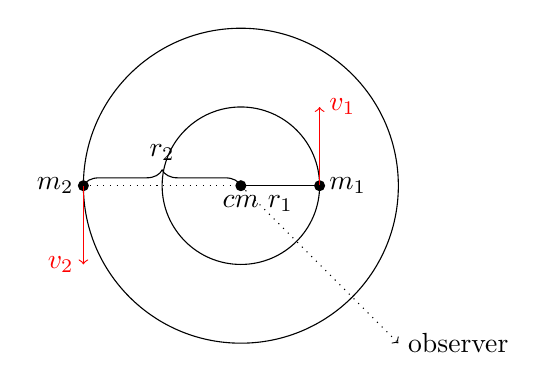
\begin{tikzpicture}

    \draw (0,0) circle (20mm);
    \draw (0,0) circle (10mm);

    \fill (-2,0) circle (2pt) node[left] {$m_2$};
    \fill (0,0) circle (2pt) node[below] {$cm$};
    \fill (1,0) circle (2pt) node[right] {$m_1$};

    \draw[red, ->] (-2,0) -- (-2,-1) node[left] {$v_2$};
    \draw[red, ->] (1,0) -- (1,1) node[right] {$v_1$};
    \draw[dotted, ->] (0,0) -- (2,-2) node[right] {observer};

    \draw (0,0) -- (1,0) node[midway, below] {$r_1$};
    \draw[dotted] (-2,0) -- (0,0);
    \draw [decorate, decoration = {brace, amplitude=2mm}] (-2,0) -- (0, 0) node[midway, above=2mm] {$r_2$};


  \end{tikzpicture}
\end{figure}
 
Via the definition of center of mass, $m_1 r_1 = m_2 r_2$.\\
We, as an observer, are somewhere in the plane of this orbit, but far away from it.

Via Kepler's third law, which we have seen before,

\begin{equation}
T^2 = \frac{4 \pi^2 (r_1 + r_2)^3}{G (m_1 + m_2)}
\end{equation}

If we measure the Doppler shift of star 1, we can find its period $T$, its velocity $v_1$, and its orbital radius $r_1$. We make a similar measurement for the second star, and find $T$, $v_2$ and $r_2$.\\
Because we then know $r_1$ and $r_2$, we obviously also know $r_1 + r_2$. We also know $T$. Using this information, using the equation above, we can find $m_1 + m_2$!\\
Not only that, but we also know that $m_1 r_1 = m_2 r_2$, so we can find $m_1$ and $m_2$ on their own, too, given that we have two equations relating the masses and orbital radii.

Using nothing but two Doppler shift measurements and some calculations, we can find the mass of each star, the radius of their orbit, how fast they move in that orbit, and the time it takes the pair to orbit once. Incredible.\\
If we are not in the plane of the orbit, however, we must have extra information: we need to know the angle $\theta$ we make with the orbital plane. We will only measure the radial components of the stars' velocities, and so only by knowing $\theta$ can we make any calculations on their actual velocities in orbit.

\subsection{X-ray binaries}

Let's now have a look at a special case of binary stars. In an X-ray binary system, we have two different types of stars: one large, relatively normal star, not too unlike our Sun.\\
The other star is a neutron star, or a black hole (or in some cases, a white dwarf). Let's assume it is a neutron star for this discussion.

Consider what happens if the two have the same mass. There will then be a point, right in the middle between them, where the gravitational pull is the same in both directions. We call this the inner Lagrangian point. If instead this point is inside the larger star, matter will fall from that star onto the neutron star, since the gravitational pull for all matter outside that point will have a stronger gravitational force towards the neutron star.

\begin{figure}[H]
  \centering
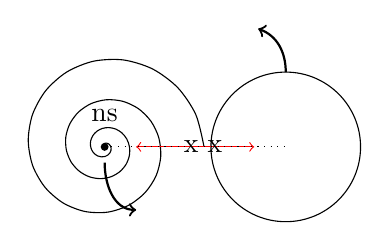
\begin{tikzpicture}
  \begin{scope}[yscale=-1]
  \draw[domain=0:25.1327,variable=\t,smooth,samples=75]
    plot ({\t r}: {0.002*\t*\t});
  \end{scope}

  \fill (0,0) circle (0.5mm) node[above=2mm] {ns};

  \draw (2.3,0) circle (9.5mm);
  \draw[red, <->] (0.4,0) -- (1.9,0);
  \draw[dotted] (0,0) -- (2.3,0);

  \draw[thick, ->] (0,-0.2) to[out=-90, in=180] (0.4,-0.8);
  \draw[thick, ->] (2.3,0.95) to[out=90, in=-20] (1.95,1.5);

  \node at (1.1, 0) {x};
  \node at (1.4, 0) {x};

\end{tikzpicture}
\end{figure}

Here, we see the larger star as the ring to the right, with the arrow indicating how it is orbiting. The neutron star is the small dot at the center of the spiral; the spiral is made up by the infalling matter, and is called the \emph{accretion disk}. Matter cannot fall radially inwards towards the neutron star, because of the fact that the two are orbiting each other (or their common center of mass, rather).

The neutron star is also called the accretor, while the larger star is known as the donor.

Consider now a small amount of matter $m$ that is released far from the neutron star. Technically, ``far'' means infinitely far away, but the answers we find are almost identical for reasonably small distances (starting out at just 1000 km from the neutron star instead of infinitely far away, the impact velocity is 99.5\% of what it is if you begin at infinity, so the impact energy is about 99\%).

We know that total mechanical energy is conserved, so the velocity of the piece that hits can be found by considering its energy as it hits, and far away, where $U = 0$ and also $K_e = 0$ (if we let it go with zero speed):

\begin{equation}
\frac{1}{2} m v^2 - \frac{m M_{ns} G}{R_{ns}} = 0
\end{equation}
\begin{equation}
v = \sqrt{\frac{2 M_{ns} G}{R_{ns}}}
\end{equation}

The kinetic energy as it hits is clearly $\displaystyle \frac{1}{2} m v^2$, where $v$ is the above impact velocity:

\begin{equation}
K_{impact} = \frac{m M_{ns} G}{R_{ns}}
\end{equation}

For $m = 10$ grams (0.01 kg), $M_{ns} = 1.5$ solar masses ($1.5 \times \SI{2e30}{kg}$) and $R_{ns} = 10$ km, we find $K_{impact} = \SI{2e14}{J}$. The impact velocity is $\SI{2e8}{m/s}$ -- ignoring relativistic effects. Keep in mind that this is for a \emph{10 gram} object! This energy output is comparable to that of the atomic bombs used in world war 2 -- all because of a 10 gram object being released from being (relatively) close to a neutron star.

There are hundreds of such systems (that are known) in our galaxy.\\
The mass transfer rate in such systems is something along the lines of $\displaystyle \frac{dm}{dt} = 10^{14}$ kg/s -- which is, of course, a rather insane number. Now, consider how much energy was released from the tiny 10 gram mass falling onto the neutron star! Here, we have $10^{16}$ times more mass \emph{per second}.\\
All in all, this gives an energy rate (power) of about \SI{2e30}{W}, about 5000 times the power output of our Sun.

Because of this enormous energy release, the temperature of the neutron star is about 10 million Kelvin. At such high temperatures, most of the EM radiation emitted is in X-rays.\\
We humans have body temperatures of about 300 K; at that temperature, we emit infrared radiation -- heat. We cannot see this radiation, but we can feel it as heat. An object at 3000 K would glow red-orange due to its temperature. At 3 million K (or degrees Celcius, which are practically the same; the difference is less than 300 K), X-rays begin to matter.

As the matter falls in, it is usually highly ionized, due to the gravitational potential energy released. Highly ionized material has electric charge, which can only reach the neutron star at certain points. The reason is that neutron stars have extremely strong magnetic fields (in particular, one sub-class called magnetars are thought to be the most strongly magnetic objects in the universe), and the movement of charged particles is affected by magnetic fields. They will tend to follow the magnetic field lines, and enter the neutron star near the two magnetic poles.

These two poles then turn into ``hot spots'', and most matter will fall in a relatively small area -- especially considering that the neutron star is very small to begin with.\\
If the axis of rotation doesn't coincide with these hot spots, we can get the effect where it rotates such that the ``jets'' created by the infalling matter appear to pulsate at us, creating an X-ray pulsar.\\
(Consider the case where it rotates around an axis that goes through its north and south (geographic) poles, while the magnetic field is perpendicular to this.)

The timing of these pulses is, as mentioned a few lectures back, extremely precise. However, now that we have a binary system, we can end up with the scenario where the neutron star is coming towards us, and then moving away from us, during an orbit (again assuming we are in the plane of the orbit). The are a bit like a clock; as it is coming towards us, due to Doppler shift, the ``ticks'' come a little closer together. As it moves away, they are a little further apart. So by timing these pulses, we can measure the Doppler shift of the neutron star, and then as earlier find the orbital radius, period and velocity of the neutron star.

If we combine that X-ray observation with an optical observation of the donor star, we see the Doppler shift in the absorption lines due to its orbit, and so we can calculate from that the donor star's orbital radius, orbital velocity and period.\\
As before, with this information, we can now also calculate the individual masses of the two stars.

In addition to what we have discussed so far, there may also be a change in activity on a longer time scale, of days rather than milliseconds or seconds.\\
If we are indeed in the plane of the orbit, then there will be times where the neutron star passes behind the donor -- and the donor then absorbs the X-ray emissions from the neutron star. This will cause periods where the X-ray activity appears to cease, until this X-ray eclipse is over.\\
This also means that we get a second, independent measurement of the orbital period.

\subsection{Chandrasekhar limit, black holes}

Of all the X-ray binaries measured so far, almost all of the neutron stars have a mass very close to 1.4 solar masses, for good reasons.\\
Indian-American physicist Chandrasekhar calculated in 1930, at the age of 19, that a white dwarf star could not exist if its mass was greater than about 1.4 solar masses. The reason lies in quantum mechanics (above that mass, the gravitational force wins over the electron degeneracy pressure, so that the star collapses -- not that I personally truly know what this means yet). This limit is known as the Chandrasekhar limit; the currently accepted value is about 1.44 solar masses.

So imagine a white dwarf, with a radius about 10 000 km. If we keep adding mass to it, by the time it reaches the Chandrasekhar limit, can collapse down into a neutron star, in a type Ia supernova.

If we instead imagine adding mass to a neutron star, by the time it reaches a mass of approximately 1.5-3 solar masses, it can yet again collapse, in this case into a black hole. This limit is known as the Tolman-Oppenheimer-Volkoff limit (or TOV limit). Similarly to the white dwarf case, a neutron star with a mass under the TOV limit is stable due to the equilibrium between two pressures, this time between the gravitational force and the \emph{neutron} degeneracy pressure.\\
As a sidenote, it is possible that other types of ultra-dense stars exist, such as quark stars. There is not yet any definite proof one way or the other, but they remain a theoretical possibility.\\
For now, let us assume that the ``next step'' from a neutron star is a black hole, and that there exists nothing in between.

What is, then, a black hole?\\
Classically, a black hole is a point mass -- it has no radius in itself. Black hole masses vary by extreme amounts for different types; it is thought that there are types from a few (3-10) solar masses, to ones with a mass of \emph{billions} of solar masses: supermassive black holes. It is also thought that most, if not all galaxies contain a supermassive black hole at their center.

A black hole does have one radius that is useful to talk about: the radius of its \emph{event horizon}. We know how to calculate escape velocities:

\begin{equation}
v = \sqrt{\frac{2 M G}{R}}
\end{equation}

As $M$ grows, there is a point that for a certain distance $R$ away, the escape velocity is the speed of light $c$. Setting the two equal, that radius is

\begin{align}
\sqrt{\frac{2 M G}{R}} &= c\\
R &= \frac{2 M G}{c^2}
\end{align}

At all points inside this radius, the escape velocity is greater than the speed of light. In other words, nothing -- not even light -- can escape, thus the term black hole. It is theoretically possible to escape from all points outside this radius, but it clearly becomes increasingly hard, the closer you come.

This radius is known as the Schwarzchild radius. All black holes have an associated Schwarzchild radius, found using the above formula. We can also use the formula to calculate into how tiny space we would need to compress a mass $M$ for it to become a black hole. Earth's Schwarzchild radius is a bit less than 1 centimeter, which says something about the insane density of black holes (even if they are not truly point masses)!

As a side note, black holes are not magical: there is a common misconception that they are the ``vacuum cleaners'' of the universe, and that they suck in everything around them. While this is true in a sense -- they do have an extremely strong gravitational pull -- they do not have any more of a pull than any other object of a similar mass.\\
If our Sun was magically replaced by a black hole \emph{of the same mass as the Sun}, all orbits in the solar system would remain unchanged. We would still die due to the lack of sunlight, but that's a different story!

Since nothing, including light (of any wavelength) can escape a black hole, how can we still observe them? In fact, \emph{can} we observe them?\\
The answer is that yes, we can. Matter in the accretion disk, that is still falling in and is still \emph{outside} the event horizon, can be observed with no contradictions. Such matter can be extremely hot, due to the release of gravitational potential energy while falling in, plus frictional forces. It can be and often is hot enough to emit X-rays.

Black holes never pulsate, as they have no surface, so you cannot have the two jets rotating around. This also implies that we cannot measure the Doppler shift of the black hole. We can measure the Doppler shift of the donor star, however. If we can also estimate the donor's mass, we can find the black hole's/accretor's mass from knowing that.

Cygnus X-1 is a famous case. It was discovered in the early 1970s. It is an X-ray binary, with an orbital period of 5.6 days. By looking at the absorption lines, astronomers estimated the donor's mass to be about 30 solar masses. (Note that this is different from what we have discussed, where we need measurements of both to \emph{calculate} the masses.)\\
The mass of the accretor must then be about 15 solar masses. Given that this is a very compact object (given that it emits X-rays), and it is clearly much more massive than $\approx 3$ solar masses, it is concluded that the object most likely is a black hole.

Since then, many other X-ray binaries have been discovered, where the accretor is thought to be a black hole.

\section{Lecture 24: Rolling motion, gyroscopes}

First out this week is rolling motion; specifically, the case where there is no slipping or skipping, which we call \emph{pure roll}.

Say we have a cylinder that is in rolling motion. It rotates with angular velocity $\omega$, while its center of mass is moving in a straight line. Say the radius of the cylinder is $R$.\\
Once it has made a complete rotation about its axis, if the distance it has moved relative to the surface below is $2 \pi R$, we call that pure roll.\\
When this is the case, the velocity $v_Q$ of the center point Q, is always the same as the tangential velocity $v_c$ about the circumference. That is, $v_Q = \omega R$ for pure roll. ($v_C = \omega R$ always holds, of course.)

If there is no friction with the surface below, we can imagine both that the cylinder might roll and roll without actually moving anywhere, and the opposite situation where it slides without rolling. In either case, then, we certainly don't have pure roll.\\
Let's now try to apply this in practice. There are no new physics here; as long as we have pure roll, we can analyze it without too much trouble.

Consider a cylindrical object on an incline of angle $\beta$. We want to calculate the acceleration of the cylinder, as it rolls down this slope with pure roll.\\
The cylinder has a mass $M$, radius $R$ and a length $\ell$.

Given two cylinders, both solid, both having the same mass and length, but differing in radii, which will accelerate faster / reach the bottom of the slope faster?\\
My semi-intuitive answer was that they both accelerate at the same rate. Considering $F = ma$ of the center of mass naively (considering only $m g \sin \beta$, the down-slope gravity), neither should win. Considering $\tau = I \alpha$ around the center, the torque is due to friction acting upwards; the larger cylinder has a larger moment of inertia (same mass, larger $R$), but it also gains a higher torque due to friction creating a torque along that longer $R$.\\
In the end, I figured the effects cancel, and $\alpha$ and $a$ are the same.

Let's look at the analytical answer. First, here is the situation will all the forces and such drawn:

\begin{figure}[H]
  \centering
  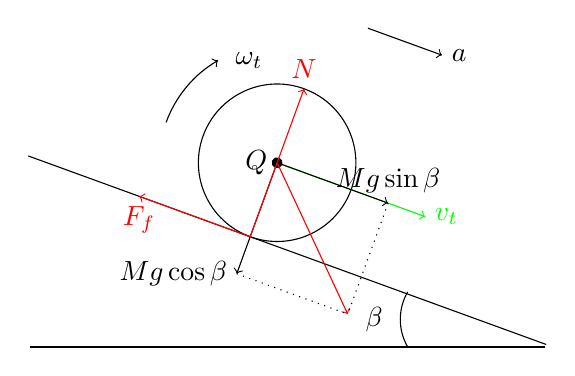
\begin{tikzpicture}
    \begin{scope}[rotate=-20]
      \draw (-3,0) -- (4,0);
      \draw (0,1) circle (10mm);

      \draw[green, ->] (0,1) -- (2,1) node[right] {$v_t$};
      \draw[->] (0.5,3) -- (1.5,3) node[right] {$a$};

      \fill (0,1) circle (2pt) node[left] {$Q$};

      \draw[->] (0,1) -- (0,-0.5) node[left] {$Mg\cos{\beta}$};
      \draw[->] (0,1) -- (1.5,1) node[above] {$Mg\sin{\beta}$};;
      \draw[red, ->] (0,0) -- (-1.5,0) node[below] {$F_f$};
      \draw[red, ->] (0,0) -- (0,2) node[above] {$N$};
      \draw[red, ->] (0,1) -- (1.5,-0.5);
      \draw[dotted] (0,-0.5) -- (1.5,-0.5);
      \draw[dotted] (1.5,1) -- (1.5,-0.5);

      \draw[->] (-1.5,1) arc[start angle=180, end angle=140, radius=1.5] node[right=1mm] {$\omega_t$};
    \end{scope}

     \draw (-2.8,-1.4) -- (3.75,-1.4);
     \draw (2,-1.4) arc[start angle=210, end angle=150, radius=0.7] node[midway, left=1mm] {$\beta$};
  \end{tikzpicture}
\end{figure}

For pure roll, we can say that the velocity of the center, point Q, must equal the tangential velocity:

\begin{equation}
v_Q = \omega R
\end{equation}

If we take the time derivative of this, we find

\begin{equation}
a_Q = \alpha R
\end{equation}

$a_Q = a$ is then the linear acceleration of the cylinder down the slope.\\
Next, we look at torque. The normal force $M g$ (since there is no acceleration in the $y$ direction, if we set $y$ perpendicular to the slope, $N = F_{gravity}$) and gravity both act through the point Q, so they cannot cause any torque. ($\vec{r}$ in the cross product $\vec{r} \times \vec{F}$ is zero, so the cross product is zero.)

The only force that does cause torque is the frictional force $F_f$, which acts perpendicularly to the center point Q. Therefore, the torque about point Q is simply $\tau_Q = R F_f$.\\
The torque must be equal to $I_Q \alpha$; Newton's second law for rotational motion is $\tau = I \alpha$.\\
Another useful relationship is $a = \alpha R$, which is just the time derivative of $v = \omega R$. Therefore, $\alpha = a/R$.

Next, we can look at Newton's second law of translation, good old $F = m a$. In this case, we have a mass $M$ on the left-hand side, and on the right-hand side, we have $M g \sin \beta$ acting downhill, and $F_f$ uphill:

\begin{equation}
M a = M g \sin \beta - F_f
\end{equation}

From the torque and all that above, we also have

\begin{align}
R F_f &= I_Q \frac{a}{R}\\
F_f &= \frac{I_Q a}{R^2}
\end{align}

With this, we can eliminate $F_f$ in the first equation and find $a$:

\begin{align}
a &= g \sin \beta - \frac{I_Q a}{M R^2}\\
a \left(1 + \frac{I_Q}{M R^2}\right) &= g \sin \beta\\
a &= \frac{g \sin \beta}{1 + \frac{I_Q}{M R^2}}\\
a &= \frac{M R^2 g \sin \beta}{M R^2 + I_Q}
\end{align}

Now we just need to enter the moment of inertia of the object, and we're done. This is the fun part. The moment of inertia of a solid cylinder, about the axis of symmetry, is $I_Q = \frac{1}{2} M R^2$. This means that $M R^2$ in the acceleration cancels!

\begin{align}
a &= \frac{M R^2 g \sin \beta}{M R^2 + \frac{1}{2} M R^2}\\
a &= \frac{g \sin \beta}{1 + \frac{1}{2}}\\
a &= \frac{2 g \sin \beta}{3} = \frac{2}{3} g \sin \beta
\end{align}

A very simple result indeed! It doesn't depend on mass, length or radius in \emph{any way}. This result is valid for all \emph{solid} cylinders (since they have the moment of inertia we used) in \emph{pure roll}.

So the answer is indeed that if we ``race'' two solid cylinders, neither one wins. We don't need to specify anything further; nothing else than ``solid'' makes any difference at all.

\subsection{Pure roll of a hollow cylinder}

What if the cylinder is hollow? Either there is a small hole in the center, or it is essentially just a thin edge, or anything in between. In this case, the moment of inertia will be larger for the same mass and radius; in the case where all mass is practically at the edge, the moment of inertia is approximately $M R^2$, i.e. twice as high. If we substitute that into the equation,

\begin{align}
a &= \frac{M R^2 g \sin \beta}{M R^2 + M R^2}\\
a &= \frac{g \sin \beta}{2} = \frac{1}{2} g \sin \beta
\end{align}

So the acceleration is now \emph{less}, so it will take longer to reach the end. Any solid cylinder will beat any hollow cylinder, regardless of their masses, lengths or radii.\\
In the case where the cylinder is hollow, but we can't approximate it either as solid or a thin edge, the moment of inertia is $\frac{1}{2} M(R_i^2 + R_o^2)$ (for inner and outer radius; the math turned too ugly with the full words as indexes). The acceleration becomes

\begin{align}
a &= \frac{M R_o^2 g \sin \beta}{M R_o^2 + \frac{1}{2} M (R_i^2 + R_o^2)}\\
a &= \frac{2 R_o^2 g \sin \beta}{3 R_o^2 + R_i^2}\\
a &= \frac{2 g \sin \beta}{3 + \frac{R_i^2}{R_o^2}}
\end{align}

This is then the most general result we can have for a cylinder. Note that when $R_{inner} = R_{inner}$, we get the one-half $g \sin\beta$ we found for the very thin cylinder. For $R_{inner} = 0$, we get the two-thirds $g \sin \beta$ that we found for the solid cylinder. I have not verified this result, but it does produce the correct answers for the two cases mentioned, so I would assume it correctly predicts the behavior in between these cases, i.e. for $R_i = (0, R_o)$, also.\\
By the way, keep in mind that this result is also, in a way, independent of geometry. Only the ratio matters; a tiny cylinder and a huge cylinder could have the same ratio $R_i^2/R_o^2$, and would then have the same acceleration.

\subsection{Gyroscopes and precession}

``We now come to the most non-intuitive part of all of 8.01. And arguably, perhaps, the most difficult part in all of physics, and that has to do with gyroscopes.''

Say we are somewhere in outer space (to escape any noteworthy gravitational force). We have a bicycle wheel with us, which is mounted such that there an axle sticking out on both sides. That is, we can hold the wheel while it rotates practically freely.

\begin{center}
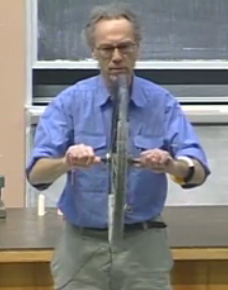
\includegraphics[scale=0.75]{\pIImages/lec24_bicycle_wheel}
\end{center}

(The reasoning for $\tau = b F$ is touched upon briefly just after the first picture in lecture 25.)

If the professor then were to push \emph{his} right hand forwards, while pulling his left right hand inwards, and apply a torque like that for a short amount of time, clearly the wheel will start spinning, counterclockwise as seen from above, and if we let it go, it will keep spinning like that forever. The torque causes a change in angular momentum, $\Delta L = \tau \Delta t$.

Next, we torque it so that the professor's left hand moves up, and his right hand moves down. This causes a rotation along a different axis, such that it spins counterclockwise as seen from our point of view (the angular velocity and angular momentum vectors are out of the screen). Again, it rotates like that forever along that axis.

Now... We spin the wheel up (along the axis a bicycle wheel \emph{should} rotate!), such that the angular velocity points to our right. What happens when he torques the wheel now?

The intuitive answer is, of course, that the wheel keeps spinning (it couldn't simply stop due to an unspecified amount of torque during an unspecified time) as a bicycle wheel does, while also rotating about the axis that we torqued it in. Without friction/air drag, both these rotations would continue on forever.

This is not what happens, though. It \emph{cannot} happen, without some external torque applied forever! The reason is that the spin angular momentum is pointing towards our right, as the experiment begins. After the torque, the intuitive answer states that this spin angular momentum would be changing direction constantly! How can a vector change direction and rotate, without any external torque? It cannot! Something else must happen.

What does happen is rather bizarre, and perhaps the most nonintuitive thing in the entire course.

As an important note on notation. any time I use ``spin'' below, I am talking about the wheel spinning like a bicycle wheel is meant to do.\\
Any time I use ``rotate'', I am talking about rotating about a different axis; one that never happens when it is attached to an actual bicycle going in a straight line.

\begin{figure}[H]
  \centering
\begin{subfigure}[b]{0.4\textwidth}
\begin{tikzpicture}[->] %(x,z,y)
  \draw (0,-2,0) -- (xyz spherical cs:radius=3) node[above] {$z$};
  \draw (0,0,-2) -- (xyz spherical cs:radius=3,latitude=90) node[above] {$y$};
  \draw (-2,0,0) -- (xyz spherical cs:radius=3,longitude=90) node[above] {$x$};

  % Cylinder Base (bottom circle)
  \begin{scope}[canvas is yz plane at x=-0.1]
      \filldraw[fill=white, draw=black, thick] (0,0) circle [radius=1.5];
  \end{scope}
  
  % Cylinder Top (top circle)
  \begin{scope}[canvas is yz plane at x=0]
      \filldraw[fill=white, draw=black, thick] (0,0) circle [radius=1.5];
  \end{scope}

  \draw[green, thick, ->] (0,1.1,0) to[out=-130, in=90] (0,0,0.9);

  \pgfmathsetmacro{\Ax}{-1.5};
  \coordinate (A) at (\Ax,0,0);
  \fill[black] (A) circle (0.4mm) node[above] {$A$};
  \draw[blue] (A) -- (\Ax,0,1) node[below] {$F$};

  \pgfmathsetmacro{\Bx}{1.5};
  \coordinate (B) at (\Bx,0,0);
  \fill[black] (B) circle (0.4mm) node[below] {$B$};
  \draw[blue] (B) -- (\Bx,0,-1) node[above] {$F$};

  \pgfmathsetmacro{\Tz}{1.8};
  \draw[blue] (0,\Tz,0) -- (0,\Tz+0.7,0) node[right] {$\uptau = \ell F$};

  \draw[red, ->] (0,0,0) -- (0.8,0,0) node[below] {$L$};

  \node at (-1.6,2,0) {$AB=\ell$};

\end{tikzpicture}
\end{subfigure}
\begin{subfigure}[b]{0.4\textwidth}
\begin{tikzpicture}[rotate around x=10] %(x,y,z)
  % Cylinder Base (bottom circle)
  \begin{scope}[canvas is plane={O(0,0,0)x(-1,0.7,0)y(0,0,1)}]
    \filldraw[fill=white, draw=black, thick] (0,0.2) circle [radius=1.5];
  \end{scope}
   
  % Cylinder Top (top circle)
  \begin{scope}[canvas is plane={O(0,0,0)x(-1,0.7,0)y(0,0,1)}]
    \filldraw[fill=white, draw=black, thick] (0,0) circle [radius=1.5];
  \end{scope}

  %\draw[green, thick, ->] (0,1.1,0) to[out=-130, in=90] (0,0,0.9);
  \draw[dashed,->] (-2,0,0) -- (3,0,0) node[right]{$x$};
  \draw[dashed,->] (0,-2,0) -- (0,3,0) node[above]{$z$};
  \draw[dashed,->] (0,0,-2) -- (0,0,3) node[below left]{$y$};

  \draw[red, -{Stealth[scale=0.5]}] (0,0,0) -- (2,1,0) node[above] {$L$};
  \draw[red, -{Stealth[scale=0.5]}] (2,0,0) -- (2,1,0) node[midway, right] {$\Delta L = \uptau \Delta t$};

  \draw[green, thick, ->] (-1.2,1.0,0) to[out=-130, in=160] (0,0,1.0);

\end{tikzpicture}
\end{subfigure}
\end{figure}


As can be seen from this picture, which describes this exact situation, the torque is upwards. The spin angular momentum will ``follow'' this torque, and \emph{tilt the wheel} so that the angular spin momentum vector gets closer to the initial position of the torque.\\
That might not sound so strange, unless you keep the conditions in mind: the professor is doing a forwards/backwards push/pull on each side of the wheel, respectively, and instead of turning in the horizontal plane, it \emph{tilts} to the side! This is something that perhaps must be seen to be believed.

It is, of course, possible to predict what will happen, when we take what we know about physics into account. One very helpful thing to remember is that the spin angular momentum vector will always ``chase'' the torque vector. In this case, the torque is upwards, while the spin angular momentum is initially towards the right. In this situation, as we have seen, the wheel tilts such that the spin angular momentum is now pointing slightly upwards, as well.\\
When we reverse the torque, so the torque is downwards, the wheel tilts in the other direction.

What if the professor were to left his right hand up, and move his left hand down? Well, the spin angular momentum is towards the right to begin with. The torque, found as $\vec{r} \times \vec{F}$, now points either towards the blackboard (into the screen), or towards the audience (out of the screen). The wheel will now rotate as we would have expected it to rotate above. When the force along the moment arm is upwards, the wheel rotates so that the right axle (as we see it) points towards the audience.

The professor then demonstrates this by sitting a a stool that is free to rotate, while applying torque as mentioned above. The result is that as long as he keeps applying that force, the stool spins. As soon as he stops, the stool stops; if he torques in the opposite direction, the stool rotates in the opposite direction.\\
This principle can also be applied in space -- many satellites have ``reaction wheels'' that can be used to rotate the satellite, e.g. to keep it pointed in a certain direction.

This slower rotation, that the wheel experiences when exposed to a torque, is called \emph{precession}.

\subsection{Precession of a bicycle wheel on a string}

Next, we change the experiment up a bit. Instead of holding the wheel, we attach a rope to the end of one axis, and one axis only, such that gravity causes a rather strong torque on the wheel, that wants to rotate it downwards (so that it can fall down and simply hang there). That is of course exactly what will happen -- as long as the wheel is not spinning.

Here's what the setup looks like:

\begin{figure}[H]
  \centering
\begin{tikzpicture}[rotate around x=5] %(x,y,z)
  % Cylinder Base (bottom circle)
  \begin{scope}[canvas is plane={O(0,0,0)x(0,1,0)y(0,0,1)}]
    \filldraw[fill=white, draw=black, thick] (0.1,0.2,0) circle [radius=1.5];
  \end{scope}
   
  % Cylinder Top (top circle)
  \begin{scope}[canvas is plane={O(0,0,0)x(0,1,0)y(0,0,1)}]
    \filldraw[fill=white, draw=black, thick] (0,0,0) circle [radius=1.5];
  \end{scope}

  %\draw[green, thick, ->] (0,1.1,0) to[out=-130, in=90] (0,0,0.9);
  %\draw[dashed,->] (-2,0,0) -- (3,0,0) node[right]{$x$};
  %\draw[dashed,->] (0,-2,0) -- (0,3,0) node[above]{$z$};
  %\draw[dashed,->] (0,0,-2) -- (0,0,3) node[below left]{$y$};

  \draw[->] (0,2,0) to[out=-190, in=90] (-0.5,1.5,0) node[below] {$\omega_s$};
  \draw[red,->] (0,0,0) -- (1.5,0,0) node[right] {$L_s$};
  \draw[green,->] (0,0,0) -- (0,-1.5,0) node[midway, right=2mm] {$Mg$};
  \draw (-2,0,-0.1) -- (0,0,-0.1);
  \draw (-2,0,0.1) -- (0,0,0.1);
  \draw (-2,0,0) -- (-2,2,0) node[at start, above left] {$P$};
  \draw (-2,0,0) -- (-2,2,0) node[at start, above right] {$r$};
  \fill (0,0,0) circle (2pt) node[above] {$Q$};
  \node at (1,1) {$R$};

\end{tikzpicture}
\end{figure}

The thicker part of the wheel is towards the viewer.

The length of the axle is little $r$, while capital $R$ is the radius of the bicycle wheel. It is attached to the rope at point P.\\
As the wheel spins, with angular velocity $\omega_s$ (s for spin; we will soon see why a subscript is needed), it has spin angular momentum $L_s$ towards the right, as shown.\\
Gravity acts on the wheel's center of mass, which is approximately at the center of the wheel. Therefore, there is a torque relative to the center point Q, $\tau_Q = (\vec{r} \times \vec{g}) M = r M g$, given that there is a right angle between the moment arm (the axle $r$) and the force.

The direction of this torque is into the blackboard.\\
Unlike the previous situation, in ``outer space'', there \emph{is} now an external torque, due to gravity, that will act on the wheel forever. Since that torque vector is directed into the blackboard, what will happen is that, again, the spin angular momentum vector will ``chase'' that torque. The wheel will keep spinning, but also rotate (precess) \emph{counterclockwise}, as seen from above.

The torque is also changing, since the direction of the axle is constantly changing! It will change in such a way that there is indeed a counterclockwise precession; that is easy to convince oneself of by using the right-hand rule, especially if you use the entire right arm.\\
Point the right arm along the initial spin angular momentum vector, i.e. straight towards the right. Curl your fingers along the torque, exactly perpendicular, downwards (since gravity acts exactly downwards). Your right thumb now points ``forwards'', which is how the wheel will rotate.\\
A small amount later in time, the spin angular momentum will have chased the torque a bit in that direction, and so you need to rotate your entire right arm a bit forwards. Gravity is still straight down, but the new torque vector is slightly rotated compared to the first, so the spin angular momentum vector will never catch up, and the will will keep precessing (in the absence of losses; in reality, it will of course eventually fall down).

So how in the world can the wheel just stay up like that? Gravity acts on it, so it must fall -- $\displaystyle a_{cm} = \frac{F_{ext}}{m}$!\\
Well, no -- there is a string tension in the problem! The net force upwards/downwards on the system is zero -- the string tension equals $M g$, so no downwards acceleration of the center of mass is necessary!\\
So there is no net force on the object. There \emph{is} a net torque, however! This string tension does \emph{not} cancel out the torque due to gravity! The reason is that the tension has no moment arm! It acts through the point P, so it cannot contribute to torque about that point. The wheel's center of mass is located $r$ away from that point, so there is a torque $r M g$ due to gravity, as we saw above.

We can calculate the precession frequency of the wheel. The result is

\begin{equation}
\omega_{pr} = \frac{\tau}{L_s} = \frac{r M g}{I_Q \omega_s}
\end{equation}

The derivation for this is in the book: chapter 22, page 22-4 and forwards.

This is now why we used the subscript on $\omega$ previously. $\omega_s$ is the angular velocity of the spin, while $\omega_pr$ is the angular frequency of the precession -- which is a much, much smaller value. The wheel will spin at several rotations per second, while it will take the wheel about 10 seconds to complete one rotation due to the precession.\\
Note that this equation is also valid as long as the spin angular momentum is way, way larger than the angular momentum due to the ``orbital'' motion about point P (the rope). The total angular momentum of the system is $L_s$ plus the component due to the orbital motion, $I_P \omega_{pr}$ (where we have not calculated $I_P$).\\
The equation holds while the wheels spins quickly, but it predicts a precession frequency that goes to infinity as the wheel's spin slows down, which clearly doesn't make sense.

This result does make sense, though. If we increase the torque, the precession frequency will also increase. That makes some sense, since the torque is trying to ``win'' over the spin angular momentum, and force it to change to follow the torque. The stronger the torque, the easier it has to do this, and make the wheel rotate/precess.\\
On the other hand, the faster the wheel spins, the harder it is to precess. That also makes sense, for the same reason. The same happens as the moment of inertia along the spin axis increases, which also makes it tougher to attempt to change the spin angular momentum.

We can attempt to calculate the period of the precession. Using the above equation, we can use $r = 17$ cm, the length of the axle; $R = 29$ cm, the radius of the bicycle wheel; $f = 5$ Hz (approximate spin frequency of the wheel) so that $\omega_s = 2 \pi f_s = 10 \pi$ rad/s. With these numbers, we find

\begin{equation}
\omega_{pr} = \frac{r M g}{M R^2 \omega_s} = \frac{r g}{2 \pi f_s R^2} \approx \SI{0.631}{rad/s}
\end{equation}

The period is as always $T_{pr} = \frac{2 \pi}{\omega_{pr}} \approx \SI{10}{s}$. So the wheel will spin with at about 5 turns per second (300 rpm), and rotate due to precession with about one turn per ten seconds.\\


%%% Local Variables:
%%% TeX-master: "../../main"
%%% End:


\section{Lecture 25: Static equilibrium, stability, rope walker}

We will begin by introducing the concept of static equilibrium. An object in static equilibrium is one that has no net force \emph{and} and no net torque (relative to any point we choose).\\
Such an object has zero linear acceleration and zero angular acceleration. In general, we will also assume they are at rest to begin with.\\
As an example, most objects on your table are likely in static equilibrium.

\begin{align}
\sum F &= 0\\
\sum \tau_Q &= 0 \text{ (any Q)}
\end{align}

For the net force to be zero, the net force must be zero along any axis by itself. Therefore, we can also use $\sum F_x = 0$, $\sum F_y = 0$ and $\sum F_z = 0$.

It might be easy to think that if the net force on a rigid object is zero, then it is in static equilibrium. That is far from true, though! If we have two forces of equal magnitude, acting in opposite directions, and they don't act along the same line, then they cause a net torque! The object will rotate, but will \emph{not} have any linear motion, since there is no net force.

\begin{center}
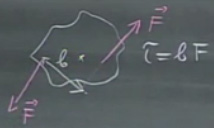
\includegraphics[scale=0.75]{\pIImages/lec25_couple}
\end{center}

(We can think of each force along causing a torque $(b/2) F \sin \theta$, where $\theta = \pi/2$ so $\sin(\theta) = 1$. They cause a torque in the same direction, so the total torque is $b F$.)

These two forces form a \emph{couple} (which I believe is a term used mostly in mechanics): together, they cause rotation, but \emph{not} translation.\\
An example of this are the forces exerted by your hand on a screw driver (or the forces exerted on the screw by the screw driver).

In this lecture, a ladder will be used for the calculations and examples regarding static equilibrium.

We put this ladder against a wall, at an angle $\alpha$ ($\alpha = 0$ meaning it is on the ground, while $\alpha = \ang{90}$ means it is standing straight up, parallel to the wall). Say there is no friction against the wall, but there is static friction $\mu$ at point Q, where the ladder touches the ground. We call the ladder's total mass $M$ and its length $\ell$.

\begin{center}
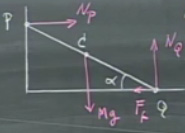
\includegraphics[scale=0.85]{\pIImages/lec25_ladder}
\end{center}

The center of mass of the ladder is in the middle.\\
Now... what forces act on this ladder?

First out, we have a gravitational force $M g$ acting on the center of mass.
 we have a normal force $N_Q$ where the ladder is in contact with the ground. Because the ladder wants to slide towards the right, there is a frictional force $F_f$ towards the left at point Q.\\
We said there is no friction at point P, so there can only be a normal force from the wall, towards the right; we call that $N_P$.

Let's now try to figure out when this static is in static equilibrium, i.e. at what angles $\alpha$ we can leave it, and have it be stable and remain at rest.\\
Our definition of static equilibrium was that the sum of all forces must be zero, and that the sum of all torques relative to any point must be zero. Let's first look at the forces.

First, in the $x$ direction. We have $N_P$ and $F_f$, so the two must be the same in magnitude.

\begin{equation}
N_P = F_f
\end{equation}

Next, the $y$ direction. Again, we have two forces, and find

\begin{equation}
N_Q = M g
\end{equation}

After this, we move on to torque. The torque relative to any point -- we can choose freely -- must be zero. If we choose point Q, neither $F_f$ nor $N_Q$ can contribute to the torque (since they act through point Q), and so we choose that point to simplify our lives.

First, we have the torque due to $N_P$. Torque is $\vec{r} \times \vec{F}$; the position vector from point Q has length $\ell$ (the entire ladder's length), and the angle between the two is $\alpha$. The cross product is then $\tau_{Q,N_P} = N_P \ell \sin \alpha$. The direction of this torque is into the blackboard, using the right-hand rule. We choose this as our positive direction, so this contributes a positive term to the net torque.

Next, there is a torque due to gravity pulling the ladder downwards. We model the gravity as acting purely at the center of mass, which is a length $\ell/2$ away from point Q. The angle between the two is not $\alpha$, but $\ang{90} - \alpha$. Therefore, the cross product becomes

\begin{equation}
\tau{Q,grav} = \frac{\ell}{2} M g \sin(\ang{90} - \alpha) = \frac{\ell}{2} M g \cos \alpha
\end{equation}

The direction is out of the blackboard, and so it contributes with a negative term. The two must be equal in magnitude, so

\begin{equation}
\sum \tau_Q = 0 \Rightarrow N_P \ell \sin \alpha = \frac{\ell}{2} M g \cos \alpha
\end{equation}

We can solve this for $N_P$:

\begin{equation}
N_P = \frac{M}{2} g \frac{\cos \alpha}{\sin \alpha} = \frac{M}{2} g \cot \alpha
\end{equation}

This must then be equal in magnitude to the frictional force, as we found earlier, or there will be a net force in the $x$ direction. This must always be smaller than the maximum possible static friction $\mu M g$, or the ladder will start to slide.

\begin{align}
\frac{M}{2} g \cot \alpha &\le \mu M g\\
\cot \alpha &\le 2 \mu\\
\alpha &\le \arctan \frac{1}{2 \mu}
\end{align}

The larger $\mu$ is, the smaller the angle can be without any sliding -- that is, the ladder can be closer to the ground, while still being held back by friction.\\
When $\mu$ is very small, it will slide at almost any angle, as we would expect. This is then demonstrated: smaller angles are less stable.

\subsection{Adding a mass along the ladder}

Let's now consider what happens when we actually use this ladder. Suppose we set it up just at the critical point, so that it is just about to slide. What happens if we stand near the bottom of the ladder, closer to point Q and far below the center of mass?\\
Will the ladder be more stable, less stable, or is there no change?

Let's consider what happens (rather quickly, as we will perform a full analysis soon). $N_Q$ will increase, which also increases the maximum possible frictional force $F_{fmax} = \mu N_Q$. This makes it seem likely that the ladder becomes more stable, as the maximum possible friction is now larger.\\
Since the actual friction $F_f = N_P$, has $N_P$ increased? I don't see why it would, so the system should become more stable.

What if the person keeps climbing, and moves past point C (the center of mass / center of the ladder), and keeps moving up towards point P? Is it now more stable, less stable, or does it not matter that the person is there?\\
Here (a bit unlike the previous case) I find it intuitively clear that this is \emph{not} a very safe thing to do. You add extra force downwards near the top of this about-to-fall ladder. This contributes to a torque that wants to rotate this ladder such that you fall down. It should also cause $N_P$ to increase, perhaps so that the required friction is now above the maximum possible. The system becomes less stable, as we will soon see.

We add a person of mass $m$ to the ladder, a distance $d$ away from point Q, measured diagonally along the ladder.

\begin{center}
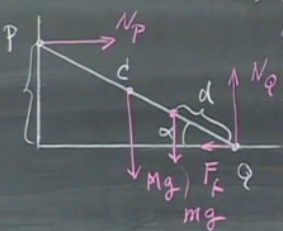
\includegraphics[scale=0.7]{\pIImages/lec25_ladder_person}
\end{center}

We then re-do the above calculations considering this extra mass.

For the $x$ direction, we still find $N_P = F_f$, as before.\\
In the $y$ direction, we have an extra downwards force, that $N_Q$ must balance out for the net force to be zero:

\begin{equation}
N_Q = (M + m) g
\end{equation}

This changes the maximum friction possible to

\begin{equation}
F_{fmax} = \mu N_Q = \mu (M + m) g
\end{equation}

which is clearly an increase from the previous case.\\
For the net torque, the first two terms are unchanged, but we add a third term due to the person of mass $m$ at distance $d$:

\begin{equation}
\sum \tau_Q = 0 \Rightarrow N_P \ell \sin \alpha = \frac{\ell}{2} M g \cos \alpha + m g d \cos \alpha
\end{equation}

The angle is calculated in the same way as last time. Again, we solve for $N_P$:

\begin{align}
N_P \ell \sin \alpha &= \frac{\ell}{2} M g \cos \alpha + m g d \cos \alpha\\
N_P \ell \sin \alpha &= g \cos \alpha \left(\frac{\ell}{2} M + m d\right)\\
N_P &= \frac{g \cos \alpha}{\ell \sin \alpha} \left(\frac{\ell}{2} M + m d\right)\\
N_P &= g \cot \alpha \left(\frac{M}{2} + \frac{m d}{\ell}\right)
\end{align}

And again, $N_P = F_f$ in magnitude, since they are the only two forces in the $x$ direction.

Since we have a new term $\displaystyle g \cot \alpha \frac{m d}{\ell}$, the frictional force has gone up. However, the maximum possible friction $F_{fmax} = \mu (M + m) g$ has also gone up!\\
In order to find which matters most, consider the case where the person is moving up the ladder gradually. To begin with, $d = 0$. We then gradually increase it. At $d = 0$, the frictional force has not changed at all, but the \emph{maximum possible} has! Therefore, the system is \emph{more stable} with this extra mass near the bottom. What happens as this mass is moving up along the ladder?

The maximum friction possible is independent of $d$, so that will always have the same, new value of $F_{fmax} = \mu (M + m) g$. However, as we climb, the actual frictional force $F_f = N_P$ (see above) does go up, due to new term we added.\\
When a certain point is reached, we are back to the just-about-to-slide situation again. If we climb higher yet, we are past that point, and the ladder will slide.

The condition we care about is that the frictional force is less than the maximum possible (when that is still the case, the ladder won't slide).

\begin{equation}
g \cot \alpha \left(\frac{M}{2} + \frac{m d}{\ell}\right) \le \mu (M + m) g
\end{equation}

However, we set the angle at the critical point we found earlier, where $\cot \alpha = 2 \mu$. We can substitute that in and solve for the largest $d$ possible for this inequality to hold:

\begin{align}
2 \mu \left(\frac{M}{2} + \frac{m d}{\ell}\right) &\le \mu (M + m)\\
M + \frac{2 m d}{\ell} &\le M + m\\
2 d &\le \ell\\
d &\le \frac{\ell}{2}
\end{align}

Quite an awesome result -- though perhaps one that could have been guessed, all things considered. Once we walk past (higher than) the center of mass, the situation is less stable that it was before. If we stand exactly \emph{at} the center of mass, we are at the just-about-to-slide stage. If we stand further down than the center of mass, the system is more stable than it was to begin with.

\section{Rope around a cylinder (capstan equation)}

We can often use friction to our advantage. One example of such a case is often used by sailors: by wrapping a rope around a cylinder, we can use friction forces as a ``substitute'' for string tension. We can have a very large force pulling on one end of the rope, which is countered in part by tension on the other side of the rope, but in larger part due to friction between the rope and the cylinder it is wrapped around.

\begin{center}
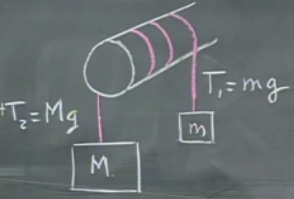
\includegraphics[scale=0.75]{\pIImages/lec25_capstan}
\end{center}

Here, we have two masses attached to either end of a rope. The middle part of the rope is wrapped several times around a cylinder.\\
If the system is at rest, $T_1 = M g$ and $T_2 = m g$. The mass $M$ is much greater than the mass $m$.

The reason the system can be at rest under these circumstances is that friction between the cylinder and the rope is trying to hold the rope in place. 

\begin{center}
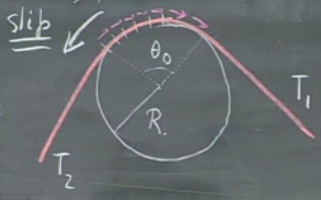
\includegraphics[scale=0.7]{\pIImages/lec25_capstan2}
\end{center}

If we consider the friction at the surface of each tiny length element of the rope, it is clear that the rope wants to slip towards the left (counterclockwise), and therefore, friction is attempting to oppose this motion. $T_2$ is pulling towards the right, but $T_1$ \emph{plus} the total frictional force is pulling towards the right. With enough friction, $T_1$ can be very small compared to $T_2$ and we can still have static equilibrium.

The result (the derivation is fairly complex and thus not shown) is that the ratio of the two tensions is given by

\begin{equation}
\frac{T_2}{T_1} = e^{\mu \theta_0}
\end{equation}

where $e^x$ is the exponential function, $\mu$ is the coefficient of static friction between the rope and the cylinder, and $\theta_0$ is the angle over which the rope is in contact with the cylinder. There is no particular limit on this angle: it could be wrapped 10 turns, which would make $\theta_0 = 20 \pi$.\\
This is known as the \emph{capstan equation}. My dictionary says that a capstan is ``a revolving cylinder with a vertical axis used for winding a rope or cable, powered by a motor or pushed around by levers''.

Notice that this result is independent of the cylinder's radius; only the angle matters.\\
The result is also exponential, so it grows extremely quickly. Adding an extra turn can make a tremendous difference in the tension ratio. For example, consider $\mu = 0.3$.

If we wrap it around exactly once, the ratio is $\displaystyle \frac{T_2}{T_1} = 6.59$ (already an impressive number). Two turns makes the ratio $43.38$, three turns $285.7$... eight turns $\num{3.54e6}$! So the first mass could be one ton, and in theory the tension from a second mass of less than one gram would be enough to counter it. Clearly, we wouldn't need to go to such extremes for this to be very useful. A mere 4 turns is enough for 1 kg to counter more than 1800 kg (or 1 N to counter more than 1800 N; since the ratio is all that matters, we can compare hanging masses in kg and tensions in newton just the same).

Let's go back to a less extreme example. If $\mu = 0.2$ and we wrap the rope 6 turns around, the ratio is about 1881, call it 2000. (If $\mu = 0.202$ instead, it goes above 2000, so it's certainly not far from it!)

With a 10 000 kg mass $M$ hanging on the left side, we could balance that force with a $\SI{10000}{kg}/2000$ = 5 kg mass on the right side! Alternatively, we could hold the rope in our hands and have no problem at all balancing this 10 ton mass on the other side.

What would happen if we let go just a little, and reduced our force from the approximately 50 newtons $(\SI{5}{kg}) g$ to just a tiny bit less? Since this ratio is for the no-slip condition, it will start to slip, and the huge mass will win, and move downwards. We can therefore control this large mass, and lower it down gently, with barely any force at all exerted by us.

What about raising the mass up? We now run in to a problem... a very, very big problem. We now want the rope to slip in the opposite direction, so that it comes towards us. This means that all those tiny friction elements between rope and cylinder switch direction, to as always oppose the relative motion between the two surfaces. To lift this object up, we must now overcome that friction \emph{and} the object's weight... so we must provide a force \emph{2000 times larger} than the object's weight in order to move it, which for a 10 ton mass is the same as hanging a 20 000 ton (20 million kg) mass on this side!\\
We should perhaps stick to lowering things down (and balancing things) using this mechanism.

This (balancing a heavy object) is then demonstrated, with a mass of approximately 30 kg hanging from a rope. After winding the rope a few times around a cylinder, the mass hangs there with almost no counterbalancing force at all. With 12 windings (perhaps even less, as 9, 10 or 11 was not tested) the weight of the remaining rather thin rope itself was enough to balance the 30 kilograms without having to even touch the rope.

\subsection{More on static equilibrium}

Consider an object of some shape (any shape), hanging on a pin somewhere (somewhere that is not through the center of mass, or the point of this will be lost).

\begin{center}
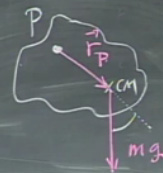
\includegraphics[scale=0.75]{\pIImages/lec25_com_position}
\end{center}

Gravity acts on the center of mass, which is not located at point P, so there will clearly be a torque. The object will start to rotate, and practically become a pendulum. Suppose we either wait until friction takes care of that, or we stop it manually. Clearly, at some point, it will reach a static equilibrium and stand completely still.

This can only happen when the center of mass is on a straight, vertical line with the point P from which it is suspended. In any other case, $\vec{r_P} \times \vec{F_{grav}} \neq 0$ and so there is a torque relative to point P, causing it to rotate.\\
More specifically, the only stable situation occurs when the center of mass is straight \emph{below} the point of suspension. Any time it is straight \emph{above}, any tiny disturbance will of course cause it to turn 180 degrees and then (once stopped) be in static equilibrium like that, instead.

We can then use this information to determine the center of mass very easily (at least in the case of a practically two-dimensional object). We hang it from one location, and draw a line from the pin (that we hang it from) and straight downwards.\\
We then move the pin to some other location, let it settle, and again draw a line straight downwards.

Since the center of mass must have been straight below the point in both two cases, there will be a unique point where the two lines intersect, where the center of mass is located!\\
Clearly, we can't find it from a single measurement: we only know that it will be straight below; it could be \emph{anywhere} straight below though (within reason -- it can't be below the lowest point of the object, of course)! With two measurements, we can narrow it down to a point on a 2D surface.

\section{Lecture 26: Elasticity and Young's Modulus}

We will now look at elasticity in materials. First, we will look at a similar situation with springs and Hooke's law.

Say we have a regular spring, with length $\ell$ and spring constant $k$. We extend it a length $\Delta \ell$ past its natural length, and according to Hooke's law, the spring force is $-k \Delta \ell$ -- a force which is trying to return the spring to its natural length. If we pull twice as hard, $\Delta \ell$ will double, and the spring force will also double.

Now, consider instead doubling the natural length of the spring. For the same pulling force, we now get twice the extension $\Delta \ell$. We can consider this as having two identical springs in series, instead of doubling the length of one, as the physics are the same. Each spring will experience the same pulling force, and so each spring individually will get longer by $\Delta \ell$. Therefore, the spring that is twice as long is extended twice as much.

If we instead have two (still identical) parallel springs, i.e. two springs are fastened at some wall, while a block or such is put on the other side and attached to each spring individually, they will have to share the load. Therefore, if we pull with a force $F$, each spring will respond with a force $-F/2$, so that the net force due to the two springs cancels out our pulling force.\\
Since they are still identical, with the same $k$, they must each be extended by only half as much as previously, so that the sum of the force due to both springs equals the pulling force.\\
If we had three springs in parallel, each would only have to provide a third of the force, and would only extend a third as much.

With these short thought experiments in mind, we have found these three relationships for these springs:

\begin{align}
\Delta \ell &\propto F\\
\Delta \ell &\propto \ell\\
\Delta \ell &\propto \frac{1}{\text{\# of springs in parallel}} \text{ (for identical springs)}
\end{align}

Let's now move on to the subject at hand. We replace the springs by rods (say metal rods, for example) with a cross-sectional area $A$ and length $\ell$. We apply a force at one end of the rod (while it is fastened at the other end, like the springs).

If we new consider this rod as a spring, pulling on this rod with a force $F$ will again extend it a distance $\Delta \ell$. As long as Hooke's law holds, i.e. that the restoring force is proportional to $\Delta \ell$, we can again say that $\Delta \ell \propto F$.

What if we put two rods together, so that the length doubles? (That is, we put them ``in series''.)\\
Again, we get the same result: each rod experience the force $F$, so each rod extends by $\Delta \ell$, and the extension doubles by doubling the length of the rod. $\Delta \ell \propto \ell$ holds for the rods, too.

Finally, what if we have two next to each other, in parallel? We pull downwards with a force $F$, that is shared by the two rods. Each rod only needs to counter half of our pull, and so they extend by $\Delta \ell/2$, just like the springs did. With twice the cross-sectional area $A$ of the rods, we get half $\Delta \ell$. Therefore, $\Delta \ell$ is inversely proportional to the cross-sectional area of the rods.

All in all, for the rods, we find

\begin{align}
\Delta \ell &\propto F\\
\Delta \ell &\propto \ell\\
\Delta \ell &\propto \frac{1}{A}
\end{align}

We can write this as a single proportionality:

\begin{equation}
\Delta \ell \propto \frac{F \ell}{A}
\end{equation}

Reordered,

\begin{equation}
\frac{F}{A} \propto \frac{\Delta \ell}{\ell}
\end{equation}

The proportionality constant $Y$ (or $E$) is called Young's modulus. The equation becomes

\begin{equation}
\frac{F}{A} = Y \frac{\Delta \ell}{\ell}
\end{equation}

Because the fraction on the right has no dimension, while the left-hand side has dimension force per unit area, which is pressure, $Y$ also has units of pressure (newtons per square meter).

In this equation, $\displaystyle \frac{F}{A}$ is called the \emph{stress} while $\displaystyle \frac{\Delta \ell}{\ell}$ is known as \emph{strain}.

If we compare two rods with different value for Young's modulus, the one with the smaller value is easier to stretch out: it gives a larger strain for a given stress. If the Young's modulus is very high, the rod is very stiff.

As an example, if we hang a mass of 500 kg of a cylindrical steel rod of radius 0.5 cm and length 1 meter, how much will it stretch? We can start by solving the equation for $\Delta \ell$:

\begin{equation}
\frac{F \ell}{A Y} = \Delta \ell
\end{equation}

$F = (\SI{500}{kg})(\SI{10}{m/s^2}) = 5000$ N. $A = \pi R^2 = \SI{7.85e-05}{m^2}$. $Y$ for steel is given as $\SI{20e10}{N/m^2}$. We find $\Delta \ell = 0.32$ mm.\\
If we instead use nylon with $Y = \SI{0.36e10}{N/m^2}$, it would stretch 18 mm.

The stress in this case is about $\SI{6.4e7}{N/m^2}$ (for either material -- it does not depend on $Y$, only on the force and the cross-sectional area).

If we keep adding more mass, there is clearly a point where the rod will simply break. That breaking point is at the \emph{ultimate tensile strength}, which is given as a pressure. In other words, when $\displaystyle \frac{F}{A}$ becomes too large, the rod breaks.\\
The ultimate tensile strength of both steel and nylon are such that neither would break given the load we calculated above; even the nylon could tolerate a few times this force. If the bar was made out of aluminium however, which has an ultimate tensile strength of about $\SI{7.8e7}{N/m^2}$, we would be rather close to the breaking point.

Before the material breaks, our equation will stop working, as the strain will no longer be proportional to the stress. Hooke's law no longer holds. If we overload the material like that, it will not return to its original length again, but will be permanently deformed. This also has an analogue with springs: pull too much on a spring, and the restoring force becomes nonlinear, and the spring will eventually be permanently deformed.

Let's have a look of what a stress vs strain plot may look like.

\begin{center}
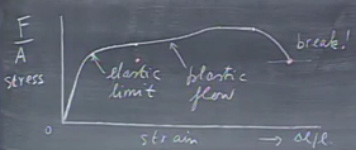
\includegraphics[scale=0.75]{\pIImages/lec26_stress_vs_strain}
\end{center}

The first part of the curve is linear: this is where Hooke's law applies. The next part of the curve is nonlinear, and goes to a point known as the \emph{elastic limit}. Even though it is not linear, as long as we do not pass the elastic limit, the material will return to its original length after we return the force.

Once we pass the elastic limit, however, the material will be permanently deformed.\\
Past this limit, increasing the stress by small amounts will cause very large amounts of strain: That is, the material will be much easier to stretch. If we then remove the force, the material would not return back to where it was. That also implies that if we create a graph like this one by gradually increasing the force and plotting $\displaystyle \frac{\Delta \ell}{\ell}$, if we gradually remove the force, the strain will not follow the curve back to zero, but will instead return to somewhere to the right of the origin.\\
The work we have done in pulling will go in part to deforming the rod, which takes energy, and in part to heat: the rod will heat up, sometimes quite substantially.

Past the elastic limit, but before the breaking point, there is a completely horizontal part of the curve. This implies that with no change at all in the stress ($y$ axis), the strain will increase anyway, and the rod will stretch without any extra force being applied. We call this \emph{plastic flow}. In this region, the material acts almost like a liquid, flowing towards the force.

Prior to breaking, the stress is lower than it was in the plastic flow region. The reason is that the material can start to pinch, so that it gets thinner at a point. That will cause the cross-sectional area to decrease, and so $\displaystyle \frac{F}{A'}$, where $A'$ is the new cross-sectional area, will be larger than $\displaystyle \frac{F}{A}$ for other points.

There are machines designed to test materials, and create plots like this one. They then increase the value of $F$ very gradually, and measure the strain. In the linear region, and the nonlinear region around the elastic limit, this is straightforward.\\
Once they start reaching the plastic flow area, however, they decrease the force. If $\Delta \ell$ increases anyway, they decrease it further. It then becomes possible to trace out the entire curve, until the breaking point.

Brittle materials generally have a curve with many of the same characteristics, but they are practically squashed together right-to-left, so that all these regions occur for smaller values of the strain.

Next we have a very long demonstration with a set-up and measuring of these values of strain vs stress, and plotting them on the blackboard. As usual, I don't really take any notes during demonstrations.

As one of many results of the demonstration, we find that in the linear region, the 36 cm copper rod has only expanded with about 0.13\%. Any further expansion was not linear, and eventually entered the plastic flow region, where adding 1 kg more (for a total of 5 kg) hanging from the copper string would \emph{double} $\Delta \ell$ -- not very linear at all!

A typical breaking point for metals would be at 5\% to 10\% extension over the original length, or so.

\subsection{Elasticity and simple harmonic oscillations}

In the linear portion, just as with springs, there is a restoring force that is linearly proportional.to the extension distance. Assuming this also holds for compression (which appears to have been silently assumed in the lecture), this forms a simple harmonic oscillator. We can solve the equation regarding the Young's modulus for $F$:

\begin{align}
F = \frac{A Y}{\ell} \Delta \ell
\end{align}

Here, we can think of $\displaystyle \frac{A Y}{\ell}$ as the spring constant $k$ (the units are indeed N/m), while as we saw earlier in the lecture $\Delta \ell$ is really just a different way of notating the displacement $x$. Stick a minus sign in there to take care of the direction (it's a restoring force), and we have an equation that is the same as that of a spring oscillator with $\displaystyle k = \frac{A Y}{\ell}$, which gives us

\begin{align}
\omega &= \sqrt{\frac{k}{m}} = \sqrt{\frac{A Y}{\ell m}}\\
T &= \frac{2 \pi}{\omega} = 2 \pi \sqrt{\frac{\ell m}{A Y}}\\
f &= \frac{\omega}{2 \pi} = \frac{1}{2\pi} \sqrt{\frac{A Y}{\ell m}}
\end{align}

For $Y = \SI{11e10}{N/m^2}$, $m = 3$ kg, $A = \SI{2e-7}{m^2}$ and $\ell = 0.36$ m, we find a frequency of about 23 Hz.

%%% Local Variables:
%%% TeX-master: "../../main"
%%% End:

%TODO: add \section{Lecture 27: Gases and incompressible liquids}

Say we have a vessel containing a fluid, where a fluid is either a liquid \emph{or} a gas\footnote{Or more rarely other states of matter; we will only discuss liquids and gases, however.}. That is, a fluid does \emph{not} refer exclusively to a liquid, unlike colloquial usage of the word.\\
It has an opening of area $A$, where we apply a force $F$.

\begin{center}
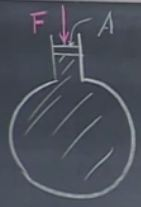
\includegraphics[scale=0.8]{\pIImages/lec27_container}
\end{center}

The pressure at the opening is by definition $\displaystyle P = \frac{F}{A}$, measured in pascal (1 Pa = 1 $\text{N/m}^2$).\\
In the absence of gravity, the pressure everywhere inside this vessel in the same; this is known as \emph{Pascal's principle}.

According to Pascal's principle, a pressure enclosed to an enclosed fluid is transmitted undiminished to every point of the fluid, and to the walls of the container.\\
Pressure is a scalar, i.e. it has no direction. Force has a direction, of course, though.\\
The force exerted on the walls of the container must, at all points, be perpendicular to the wall, in a static situation.\\
If there was a tangential component to any such force, that net force would cause movement in the fluid, and we are no longer in a static situation.

As a result of this, for a small area element $\Delta A$ of the container, we can relate the force on that area $\Delta F$ with the pressure:

\begin{equation}
P = \lim_{\Delta A \to 0} \frac{\Delta F}{\Delta A}
\end{equation}

Pascal's principle leads has many interesting consequences, some of which are not very intuitive. First, we shall look at a hydraulic jack.

\subsection{Hydraulic jack}

We have a container, containing a fluid (a practically incompressible liquid); see drawing:

\begin{center}
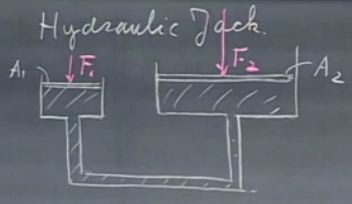
\includegraphics[scale=0.8]{\pIImages/lec27_hydraulic_jack}
\end{center}

The left side has a piston of area $A_1$, and the right area a piston of area $A_2$.\\
We apply a downwards force $F_1$ on the left side, and a downwards force $F_2$ on the right side.

According to Pascal's principle, the pressure everywhere in this container is the same. Since the pressure below each piston is that force divided by that piston's area,

\begin{equation}
P = \frac{F_1}{A_1} = \frac{F_2}{A_2}
\end{equation}

when the liquid is not moving. This is also assuming we can neglect gravity, which we will discuss shortly.

We can then design this system such that $A_2/A_1 = 100$. Rearranging the equation,

\begin{equation}
\frac{A_2}{A_1} = \frac{F_2}{F_1}
\end{equation}

We could then have the situation where $F_2 = 100 F_1$, so that we could balance out a very large force with a much smaller one -- similarly to a capstan.

Unlike a capstan, we can use this system to lift very heavy weights easily. We could put a mass of 10 kg on the left piston, and a mass of 1000 kg on the right, and the system would be in equilibrium.\\
This is used, for example, to lift cars. As we expect, if we increase the force $F_1$ a small amount, that piston will go down, which will force the other to go up, lifting the heavy object using a much smaller force.

So how does this work in regards to energy?\\
Well, consider we push the left piston down a distance $d_1$. We displace a volume $d_1 A_1$ of fluid. This fluid has nowhere to go but the right side, where it moves the right piston a distance $d_2$, displacing a volume $d_2 A_2 = d_1 A_1$.

Using the above equation,

\begin{equation}
d_2 = d_1 \frac{A_1}{A_2}
\end{equation}

And since $A_2 > A_1$, we see that we must push $d_1$ down a lot to raise $d_2$ a little. In other words, the work we do, $F_1 d_1$, is equal to the work done at the right side, $F_2 d_2$, assuming no losses.\\
With this ratio, you would have to move the left piston a distance $d_1 = 100$ m, to raise the right piston $d_2 = 1$ m -- rather unpractical if you want to lift a car, for example.\\
However, we can design such a jack so that we can move it a short distance by applying a force with a lever, and then lower it down again, and repeat. This way, we only raise the car (or whatever we are trying to lift) a very small distance at a time, perhaps less than a centimeter, but can repeat the process until we reach the height we want.

\subsection{Pressure due to gravity: hydrostatic pressure}

Until now, we ignored the effect gravity would have on such a system; we will now (essentially for the rest of the lecture) discuss pressure in fluids in the presence of gravity.

Consider a liquid inside some container. We will look at a small ``slab'' of liquid, which is then everywhere surrounded by more of that same liquid.\\
We look at a piece of area $A$, height $\Delta y$ and density $\rho_y$ -- i.e. the density may be a function of $y$.

We have increasing values of $y$ upwards. The call the coordinate at the bottom of the slab $y$, and the one at the top is then $y + \Delta y$.\\
The pressures at the two depths are then $P_y$ and $P_{y + \Delta y}$, respectively.

\begin{center}
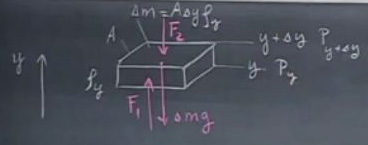
\includegraphics[scale=0.8]{\pIImages/lec27_hydrostatic}
\end{center}

The mass of this ``element'' of liquid is $\Delta m = A \Delta y \rho_y$, i.e. simply the volume times the density.\\
Now, what are the forces on this element? First, there is gravity, $\Delta m g$, acting downwards. There is then a force $F_1$ upward, due to the pressure on this element. Keep in mind that the pressure is everywhere perpendicular to a surface -- even on imaginary surfaces like this one.\\
It then also comes in from the top, with force $F_2$. The forces in the horizontal plane all cancel.

For there to be equilibrium, we apply Newton's second law:

\begin{equation}
F_1 - F_2 - \Delta m g = 0
\end{equation}

By definition, $F_1$ is the pressure at that level, times the area, $F_1 = A P_y$. For the same reasons, $F_2 = A P_{y + \Delta y}$.\\
We can then substitute in the expression we had for $\Delta m$, and find

\begin{align}
A P_y - A P_{y + \Delta y} - A \Delta y \rho_y g &= 0\\
P_y - P_{y + \Delta y} - \Delta y \rho_y g &= 0\\
- \Delta y \rho_y g &= P_{y + \Delta y} - P_y\\
- \rho_y g &= \frac{P_{y + \Delta y} - P_y}{\Delta y}
\end{align}

$A$ cancels, and we can then rearrange this a bit, as shown above. Finally, we can take the limit as $\Delta y \to 0$ and we see that what we have is the definition of a derivative,

\begin{equation}
\lim_{\Delta y \to 0} \frac{P_{y + \Delta y} - P_y}{\Delta y} = - \rho_y g \Rightarrow \frac{dP}{dy} = -\rho_y g
\end{equation}

This equation shows us the definition of \emph{hydrostatic pressure}. As the equation tells us, hydrostatic pressure is there because of gravity.

Most liquids are in practice almost completely incompressible, meaning that the density is practically constant, so we can really change $\rho_y$ into $\rho$ above.\\
Even at an ocean depth of 4 km, at pressures of almost 400 times atmospheric pressure (400 atm is about $\SI{4000}{N/cm^2}$) the decrease in volume of water is less than 2\%. Gases, on the other, are often very compressible.

Say we have a liquid in a container, and apply a force on the top (like in the case we had in the beginning of the lecture), we could not get a measurable change in the density using any reasonable force we as humans could apply. With machines, of course, we absolutely could compress it.

If we hit an air-filled plastic pillow with a sledgehammer, the air would act as a cushion. If we instead hit a marble floor, the pressure on the sledgehammer (and on the floor) would be way higher than that of the pillow, since the marble floor is almost completely rigid and incompressible, so this ``cushioning'' effect is gone.

Now consider two metal paint cans. One is completely filled with water (with no air at all inside), while another is filled with air (at atmospheric pressure).\\
If we hit these two cans with a sledgehammer, there would again be a cushion effect one the one filled with air, while the force (and pressure) on the one filled with water would be much higher.

If we now fire a bullet into these containers instead, what happens? The area where the bullet hits is very small, but the force is clearly very high. With these two effects in combination, the pressure will be extremely high.\\
Pascal's principle says that the pressure will propagate undiminished in the fluid.\\
In the one filled with air, there is not much of a problem: the air is glad to change its volume/density to take care of this.\\
In the one filled with water, however, the pressure is extremely high, and the can may will explode due to the extreme pressure on the sides of the can, as the water won't compress any noticeable amount.

\subsection{Pascal's law}

From now on, we will assume that liquids are completely incompressible.\\
With that in mind, we can now treat $\rho$ as a a constant, and calculate the pressure change as a function of a change in depth, via separation of variables. Again, considering that $+y$ is upwards, and $y_2 > y_1$ (below),

\begin{align}
\frac{dP}{dy} &= - \rho g\\
\mathop{dP} &= - \rho g \mathop{dy}
\end{align}

We can integrate both sides, from $y_1$ to $y_2$ and $P_1$ (pressure at $y_1$) to $P_2$ (pressure at $y_2$) respectively. $g$ is also constant, so the integrals are just the integrals of the differentials themselves (think of it as $\int_a^b 1 \mathop{dx}$).

\begin{align}
\int_{P_1}^{P_2} \mathop{dP} &= - \rho g \int_{y_1}^{y_2}\mathop{dy}\\
P_2 - P_1 &= -\rho g(y_2 - y_1)
\end{align}

Equivalently, we can multiply both sides by $-1$ and get

\begin{equation}
P_1 - P_2 = \rho g(y_2 - y_1)
\end{equation}

which you may or may not prefer.\\
This result is known as \emph{Pascal's law}.

Consider a strange-shaped vessel containing a liquid:

\begin{center}
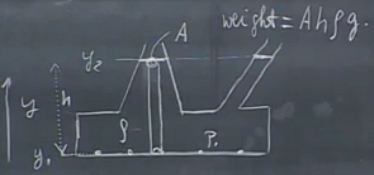
\includegraphics[scale=0.7]{\pIImages/lec27_strange_container}
\end{center}

According to Pascal's law, the pressure at the bottom must be the same, at all points along the bottom (assuming the liquid is static).\\
However, consider the point just below the marked cylinder: the water column has a weight $A h \rho g$ -- its volume $A h$, times the density $\rho$ which gives its mass, times $g$ which gives its weight. The pressure at the bottom is this weight divided by the area, i.e $\rho h g$.

However, the pressure just below that column must be exactly the same as the pressure in the corner, where the water column above is much smaller. Not that intuitive.\\
If we think of it in terms of requiring no net force for a static situation, it does make sense, but from the perspective of weight, it does not.

What is the pressure difference due to gravity for a water column that is 10 meters high?

Well, using $P_2 - P_1 = \Delta P$ and $y_2 - y_1 = \Delta y$ we find, using the previous formulas, $|\Delta P| = \rho g \Delta y$.\\
$\rho$ for water is $\SI{1}{g/cm^3} = \SI{1000}{kg/m^3}$. Using $g = \SI{10}{m/s^2}$ and $\Delta y = \SI{10}{m}$, we find $\Delta P = 10^5$ Pa, which incidentally is very close to 1 atmosphere of pressure (i.e. the pressure the air exerts on us, all the time), which is defined as 101325 Pa; more on that soon.\\
This is a very useful thing to remember: there is an additional 1 atm of pressure for each 10 meters you go down in water.

\subsection{Atmospheric pressure and barometers}

``We live at the bottom of an ocean of air'', as the professor says.

Unlike liquids, the density of air changes noticeable with altitude (clearly: as we go up, sooner or later, the density is almost exactly zero, out in space, and the change is gradual), so we can't do the very simple integration we did earlier with the $\rho$ of air.\\
We can weigh it, though. Look back to the case of the strange-shaped vessel with water: the pressure at the bottom, below a column of water stretching all the way up, was the same as the weight of that column, divided by the area.

In the same way, if we weigh a column of air stretching up to the edge of the atmosphere, we would measure a weight of approximately 10 N per square centimeter. There are 10000 square centimeters in a square meter, so the pressure is about $10^5 \text{N/m}^2 = 10^5 \text{ Pa}$.

More exactly, atmospheric pressure is, as mentioned earlier, defined to be exactly 101325 Pa. It varies with the weather, altitude, etc., but is often relatively nearby. In my case, living within 25 m of sea level, I find it rare to look at a barometer and see a value outside the range 970-1030 hPa (i.e. 97000-103000 Pa).

If we hold out our hands, we feel a force equivalent to about 150 kilogram-force or kgf\footnote{1 kgf = 1 kg times $\SI{9.80665}{m/s^2}$; the unit is used so that we can talk about forces in terms of kilograms, which are more familiar in daily usage than newtons.} pushing downwards.\\
However, there is also a force of almost exactly equal magnitude pushing up on the hand's underside, as well as horizontal forces in many directions. All of these forces are, as mentioned earlier, exactly perpendicular to the hand, if the air is not moving.

We can measure the atmospheric pressure in a rather different way. We emerge a hose completely in a liquid of known density, and block off the the top end. The liquid will stay inside the tube, so that it is filled all the way, up to a certain height. For water, this height is about 10 meters; at that point, the liquid ``lets go'' and the very top of the tube will contain a vacuum.

Consider now instead a glass tube instead of a hose, and mercury instead of water. Mercury is way denser than water, so the height required will also be way less than the 10 meters required for water.

\begin{center}
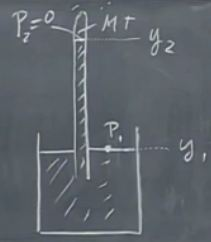
\includegraphics[scale=0.8]{\pIImages/lec27_barometer}
\end{center}

(MT means empty, nothing more; I'm not sure why it is written in short.)

$P_1$ is clearly just the atmospheric pressure, since it is in direct ``contact'' with the outside air.\\
A distance $y_2 - y_1 = h$ above, the pressure is $P_2 = 0$, since there is a vacuum.

We have the formula $P_1 - P_2 = \rho g(y_2 - y_1)$, but since $P_2 = 0$ and $P_1$ is the atmospheric pressure, using the definition of $h$, we have

\begin{equation}
P_{atm} = \rho g h
\end{equation}

where $h$ then is the height of the column of mercury. This device is known as a \emph{barometer}.\\
Using $P_{atm} = 101325$ Pa as an example (it can clearly differ), combined with $g = \SI{9.81}{m/s^2}$ and $\rho = \SI{13.6e3}{kg/m^3}$, we find that the height of the column will be about 760 mm.\\
Because mercury barometers were quite common in the past, this pressure is often referred to as 760 mmHg. Other pressures are also measured in mmHg -- ``millimeters of mercury''; blood pressure is almost always measured in mmHg (the ``golden standard'' of approximately 120 over 80, for example, is measured in mmHg).

For water, using the same formula, we see that the column would then have to be about 10 meters high (as mentioned earlier), which is impractical, yet possible.

\subsection{Submarines and hydrostatic pressure}

Construction of the world's first submarine is usually credited to Dutchman Cornelius van Drebbel, as early as 1622. He not only built it, but successfully operated it at a depth of 5 meters, where the hydrostatic pressure is about 0.5 atmospheres. Add to that the atmospheric pressure of 1 atmosphere, and you get a total pressure of 1.5 atm at that depth.

Since he had 1 atmosphere of air inside, to breathe, the pressure differential is then 0.5 atmospheres, equivalent to about 50 kPa or 5000 kgf per square meter acting on the outside; very impressive for the time.

The professor mentions that modern submarines have gone down to at least a 900 meter depth, meaning approximately 90 atmospheres of hydrostatic pressure, but for some reason made no mention of the manned descents into the Challenger Deep (once in 1960, once in 2012; the latter was after the lecture was recorded, however) to a depth of about 10920 meters! The pressure down there is over \emph{a thousand} atmospheres, equivalent to over $10^8$ Pa, or equivalent to having over ten thousand metric tons of mass on each square meter of the outside, in Earth's gravitational field that is. The fact that this is not only possible, but was done even before the first moon landing, amazes me quite a lot.\\
These descents are not done in regular submarines, of course, but they are still man-made vessels that can withstand such absurd pressures.

The professor demonstrates what a ``small'' pressure difference of 0.5-1 atm can do to an object, by sucking the air out of a paint can. There will then be an underpressure inside the can, i.e. the pressure is larger outside than inside.

Long before the pressure difference is 1 atm (i.e. before there is a vacuum inside the can), it has already crumpled up quite a lot. Based on what happens, it's fairly safe to say that this paint can wouldn't survive at a 5 meter depth, if filled with 1 atmosphere of air and then hermetically sealed. 

Now, consider what happens when we go scuba diving. Could we snorkel at a 10 meter depth? Far from it, actually!\\
The air in our lungs would be at 1 atm, connected to the surface via a snorkel (or a simple hose, etc). The pressure on our chests from the outside would be about 2 atm, however, since there is a hydrostatic pressure of 1 atm in addition to the atmospheric pressure of the air at the surface.

Since 1 atm is about 100 kN per square meter, or 10 tons worth of weight, raising your chest to breathe in is absolutely impossible under these conditions. If you can't breathe with a car standing on your chest, how could you breathe with an equivalent hydrostatic force of the same magnitude pushing in on you? (Based on a chest size of about a tenth of a square meter, or so, the force will be about one ton's worth of weight at $g$.)\\
So at what depths \emph{could} we snorkel?

Well, to answer the question, we would need to know approximately what sort of underpressure we can have in our lungs, and still be able to breathe in. It seems reasonable, but tough, that we could perhaps lift a 100 kg weight laying on our chests, using only our lungs. I doubt that it's easy, but it's probably doable, at least for some humans.\\
Given a chest area of 0.3 times 0.3 meters, or 0.1 square meters, this is equivalent to a pressure of about $\displaystyle \frac{(\SI{100}{kg})(\SI{10}{m/s^2})}{\SI{0.1}{m^2}}$, or about 10000 Pa.\\
That is, the outside pressure cannot be more than 10000 Pa greater than atmospheric pressure; that is about 0.1 atmospheres.

At what depth is the hydrostatic pressure 0.1 atm? With the rule of 1 atm per 10 meters, this is at about 1 meter, or so. So a roughly calculated answer is than snorkeling at a depth greater than 1 meter is essentially impossible.\\
We will look at this in more detail now.

By the way, the way divers get around this is to have pressurized breathing gas. That is, the air in their lungs is at about the same pressure as the water outside.

\subsection{Manometers}

A manometer is a very simple device that can be used to measure pressure. We have a U-shaped tube, plastic in this case, which is partially filled with water.

\begin{center}
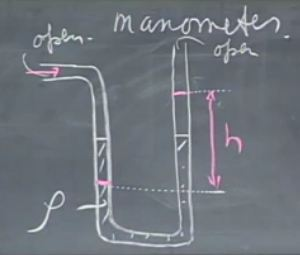
\includegraphics[scale=0.8]{\pIImages/lec27_manometer}
\end{center}

By blowing (or sucking) on one end, we can measure the height difference in the liquid, and calculate the amount of underpressure/overpressure we managed to produce in our lungs.\\
Call the top height $y_2$ with pressure $P_2$, and the bottom $y_1$ with pressure $P_1$, we have

\begin{equation}
P_1 - P_2 = \rho h g
\end{equation}

$P_2$ is at atmospheric pressure, since it is connected to the outside world. Therefore, solving for $P_1$ and making a substitution,

\begin{equation}
P_1 = \SI{1}{atm} + \rho h g
\end{equation}

So we can measure the amount of pressure we can generate above or below the atmospheric pressure. We call that overpressure and underpressure, respectively.\\
If you have ever measured the pressure in a car's tires, that is done by an overpressure gauge.

If we use water in the manometer, the height difference it shows is equal to the depth at which we could snorkel (for a short amount of time, at least), since 1 meter on the manometer means we can generate an overpressure of 0.1 atm, and the hydrostatic pressure at such a depth also is 0.1 atm.\\
The hard part of snorkeling is breathing \emph{in}, though -- out is easy, since your lungs are compressed from the outside. In other to find out out maximum snorkeling depth, we need to measure the maximum \emph{underpressure} we can produce, i.e. when sucking.

The professor then demonstrates this, and then demonstrates an interesting feat: drinking with a ``straw'' that is much, much longer than the 1 meter he could manage with the manometer. Exactly how it's done is not explained.

\section{Lecture 28: Hydrostatics, Archimedes' principle, and fluid dynamics}

We will now look at how objects float.\\
Say we have a cylinder of end-cap area $A$ and length $\ell$, and therefore volume $A \ell$. It has a uniform density $\rho$, and therefore a mass $M = A \ell \rho$.\\
The cylinder is in a liquid of density $\rho_{fl}$, and a height $h = y_2 - y_1$ of the cylinder is submerged.

\begin{center}
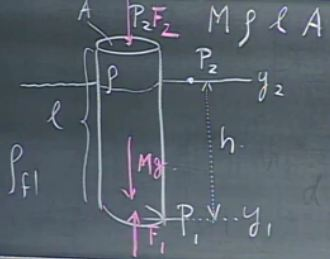
\includegraphics[scale=0.8]{\pIImages/lec28_floating_cylinder}
\end{center}

There is a downwards force $F_2 = A P_2$ due to the weight of the air above the cylinder, and an upwards force $F_1 = A P_1$ due to the hydrostatic pressure. �n addition, there is a gravitational force $M g = A \ell \rho g$ downwards.

Via Pascal's law, $P_1 - P_2 = \rho_{fl} g h$.

In equilibrium, the forces on the cylinder must be balanced:

\begin{equation}
F_1 - F_2 - M g = 0
\end{equation}

If we multiply both sides of the Pascal's law equation by $A$, we find

\begin{equation}
A P_1 - A P_2 = A \rho_{fl} g h
\end{equation}

The left side here, $A P_1 - A P_2 = F_1 - F_2$, is known as the \emph{buoyant force}. The other side is the \emph{weight of the displaced fluid}: $A h$ is the volume of the the displaced fluid, times $\rho_{fl}$ gives us the mass, and times $g$ times us the weight.

This is a case of \emph{Archimedes' principle}, which can be stated as: ``the buoyant force on an emerged body has the same magnitude as the weight of the fluid which is displaced by the body''.

The story is that Archimedes was given the task to find out whether a crown made for his king was made of pure gold. He therefore wanted to measure the density of the crown -- but how does one measure the density of something without destroying it? The simple solution would be to measure the volume and the weight, and then calculate the mass and density from there. However, measuring the volume of such an irregularly shaped object with e.g. a meter stick is no easy task!

What he realized (according to the legend, when he noticed the water rise as he stepped into a bath) was that he could measure the volume by submerging the crown in water.\\
Silver has a lower density than gold, so if part of the crown was silver, for a given mass/weight, it would have to be slightly larger in volume. Measuring the weight is relatively easy, but even then, measuring a fairly small change in volume is still not easy, as the change in water level would be very small (probably less than 1 mm, depending on the container size etc.). Not only that, but there could be other factors causing trouble, such a surface tension, which may well make the difference completely impossible to measure.

What one can do is the following. First, we weigh the crown as per usual, perhaps using a spring, and find a weight $W_1 = V \rho g$, where $V$ is the volume of the crown.\\
Next, we submerge it in water, and weigh it there. Because of the buoyant force acting on the crown, its weight is less under water. (Its \emph{mass} is of course the same.)

In water, the weight is the original weight, minus the buoyant force $V \rho_{fl} g$, which is the weight of the displaced fluid of volume $V$. So we have

\begin{align}
W_1 &= V \rho g\\
W_2 &= V \rho g - V \rho_{water} g = W_1 - V \rho_{water} g
\end{align}

We can solve this to find

\begin{equation}
\rho = \frac{W_1}{W_1 - W_2} \rho_{water}
\end{equation}

and also

\begin{equation}
V = \frac{W_1 - W_2}{g \rho_{water}}
\end{equation}

All of the things needed to find $\rho$ was either known ($\rho_{water}$) or easily measurable (the weights), with rather high accuracy.

\subsection{Floating and icebergs}

I'm sure most of us have heard the expression ``that's just the tip of the iceberg''. There's a good reason for that expression, as we will see now.

Consider an iceberg of mass $M$, volume $V_{tot}$, density $\rho_{ice} = \SI{0.92}{g/cm^3}$, compared to $\rho_{water} = \SI{1}{g/cm^3}$.\\
Because it is floating, the buoyant force is equal in magnitude to $M g = V_{tot} \rho_{ice} g$. The buoyant force is given by the weight of the displaced water, $F_b = V_{sub} \rho_{water} g$, where $V_{sub}$ is the volume of the iceberg that is submerged, i.e. under water.

\begin{equation}
V_{tot} \rho_{ice} g = V_{sub} \rho_{water} g
\end{equation}
\begin{equation}
V_{tot} \rho_{ice} = V_{sub} \rho_{water}
\end{equation}

$g$ cancels. We can rearrange the equation:

\begin{equation}
\frac{V_{sub}}{V_{tot}} = \frac{\rho_{ice}}{\rho_{water}} = 0.92
\end{equation}

So the submerged volume is going to be 92\% of the total volume: 9/10 of the iceberg is under water, and we can indeed only see the tip of it from above water.

Going back to our cylinder from the beginning of the lecture, what is the condition for floating? We know already that the buoyant force must equal the weight, and we have already learned that the buoyant force is equal to the weight of the displaced water, $A h \rho_{fl} g$, where $h$ is the height of the part of the cylinder that is under water.\\
That must be equal to the weight of the cylinder, $A \ell \rho g$, so after cancelling $A$ and $g$ we have

\begin{equation}
h \rho_{fl} = \ell \rho
\end{equation}

However, $h < \ell$ must be the case: the amount submerged must be less than the total height, or it would be entirely underwater. With that condition, to balance the two sides out to be equal, it must also be the case that

\begin{equation}
\rho_{fl} > \rho
\end{equation}

Very simple, indeed. Things float if their density is smaller than the density of the fluid they are in. Note that the masses or weights don't matter: a small pebble, say a 2 mm radius ``rock'', will sink in water, because rock has a greater density than water. A 1 km radius iceberg, with a mass of over $10^{12}$ kg would float in water, however, since the density of ice is smaller than the density of water.

Let's now consider an interesting question. We are in a boat, in some small-ish reservoir of water, like a swimming pool. We have a large/heavy rock in the boat with us. If we throw this rock overboard, so that it sinks, will the water level in the pool go up, go down, or stay the same as it was when the rock was inside the boat?

When it is in the boat, the boat displaces extra water due to the weight of the rock, $W = V \rho_{rock} g$, which causes the water level to rise (compared to the rock not being there at all).\\
When it is in he water, it displaces water equal to the volume of the rock; the displaced water then has a weight $V \rho_{water} g$.\\
So which is greater? The rock's weight is $V \rho_{rock} g$, while the weight of the displaced water in case is $V \rho_{water} g$. The former is clearly greater, since the rock 's density is much greater than the density of water.

More water is therefore displaced when the rock is in the boat, and so the water level will go \emph{down} when it is instead in the water.

\subsection{Stability of immersed objects; balloons}

Consider a floating object, which has a center of mass not aligned with its geometrical center. Perhaps it's an iceberg with some rocks in it.

\begin{center}
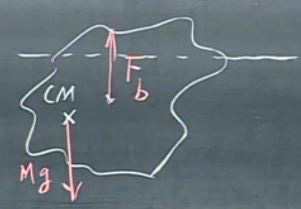
\includegraphics[scale=0.7]{\pIImages/lec28_iceberg_torque}
\end{center}

Gravity acts at the center of mass, as usual, but the buoyant force does not! It acts at the center of mass \emph{of the displaced fluid}, which is this case will be to the right of the iceberg's center of mass. Therefore, these two forces create a counterclockwise torque, causing the object to rotate.

Just as we saw previously, with an object on a pin, it will rotate until these forces are vertically aligned, so that is no longer any net torque.\\
Also as we saw previously, there are two possible cases where this happens: one where the center of mass of the iceberg is \emph{above} the point of application of the buoyant force, which would be a case of unstable equilibrium, or the more stable case where it is \emph{below}.

This is then a very important issue in the construction of ships. If a ship were to have the center of mass above the point where the buoyant force is applied, it could very easily capsize (flip around upside down). The lower the center of mass is, the more stable a ship will be.

Next, let's have a quick look at balloons, specifically ones with light gases inside, such as helium. What is the condition for them to float and rise in air?\\
Well, the situation is really very similar to an object floating in water.

The balloon has a certain mass $M$, given by the mass of the gas inside $V \rho_g$ plus the mass of the ``rest'', i.e. the balloon itself (the rubber, perhaps a string, etc). It then has a weight $W_{balloon} = g(V \rho_g + M_{rest})$.\\
In order to rise, the buoyant force must be greater than this weight. The buoyant force is given by the weight of the displaced fluid -- and the fluid is air, here. $W_{air} = V \rho_{air} g$, so the condition is

\begin{align}
V \rho_{air} g &> V \rho_g g + M_{rest} g\\
V \rho_{air} &> V \rho_g + M_{rest}
\end{align}

It's clear, then, that $\rho_g < \rho_{air}$ must be the case. That is necessary, but not sufficient: it is sufficient only for a massless balloon. Since the rubber has a small mass, the density of the gas must be smaller by a margin wide enough to also carry that mass.

\subsection{Helium balloon in an accelerated frame}

We will now look at a second example involving helium balloons. I will shorten this section compared to the lecture, which should (as always) be watched anyway, especially as this is a demonstration.

In short: in the presence of air, a helium balloon will always move in the direction that opposes gravity. That includes perceived gravity, for example due to a rocket accelerating in outer space.\\
So say we have a sealed-off ``room'' somewhere in outer space, where the gravity due to the surrounding stars etc. is completely negligible. We accelerate this system, say ``upwards'' (as shown in a drawn figure, that is). We will perceive gravity in the opposite direction, which means we will fall down, as will the air inside the room. However, as the air will sink down due to its weight (which was zero prior to the acceleration), we will essentially end up with an atmosphere inside. The pressure will be higher near what has now become the floor, and smaller at the roof. Therefore, the helium balloon will rise towards the roof, in the \emph{same} direction of the acceleration.

So far, this is a bit strange perhaps, but it still appears reasonable, since acceleration creates perceived gravity, which we cannot really tell apart from ``regular'' gravity.\\
However, now consider doing this in a room here on Earth, only we accelerate it towards the right, rather than up.\\
We have a closed compartment filled with air; it indeed needs to be closed, since this effect relies on the pressure difference between the two sides.

If we hang an apple from a string, we know what will happen: accelerate the box towards the right, and the apple will resist this motion, and appear to lean to the left.\\
However, what if we have a helium balloon, attached to the floor via a string? Before we push, it will happily float and just sit there, trying to move opposite gravity, but being stopped by the downwards tension in the string. When we accelerate the box towards the right, the air inside this closed compartment ``falls'' towards the left. Again, a pressure difference is created, such that the pressure at the left side is greater than the pressure on the right side.\\
This causes a horizontal buoyant force, and the balloon will ``float'' and move \emph{towards the right}.

That is, unlike what we would expect any object to do, it moves \emph{forward}, along with the acceleration. This can also be replicated in a car, for example. Step on the gas, and the balloon will move forward, while the passengers are pushed back into their seats; slam the brakes, and the balloon will move backward, while everyone moves forward. Not very intuitive.

\subsection{Bernoulli's equation}

We will now show a rather fast derivation of Bernoulli's equation for incompressible fluids.

Say we have a flow between two different heights, with two different areas, pressures and fluid velocities, as follows:

\begin{center}
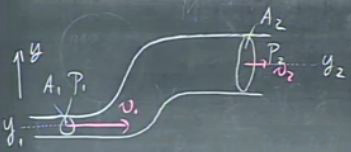
\includegraphics[scale=0.8]{\pIImages/lec28_bernoulli}
\end{center}

Because the fluid is incompressible, the amount of fluid that passes though $A_1$ per unit time must be the same as the amount that passes through $A_2$ per unit time; that is, $A_1 v_1 = A_2 v_2$. For that reason, in this case, $v_1 > v_2$.

In the case where the fluid is static, $v_1 = v_2 = 0$, we could apply Pascal's law: $P_1 - P_2 = \rho g (y_2 - y_1) = \rho g h$, using the usual definition $y_2 - y_1 = h$.\\
This then implies that the pressure at $A_1$ is higher than the pressure at $A_2$, since it is at a lower level, which implies higher pressure.

We know $m g h$ as being a term of gravitational potential energy. However, $m$ divided by volume gives us density $\rho$; therefore, the above expression is in terms of gravitational potential energy per unit volume, $\displaystyle \frac{m g h}{V} = \frac{m}{V} g h = \rho g h$.\\
Since we can only equate quantities that have the same dimension, the dimension of pressure must be the same as energy per unit volume.

If we now consider the dynamic case, where the velocities come in to play, we also have kinetic energy to consider. We can then relate the kinetic energy per unit volume, $\displaystyle \frac{1}{2} \frac{m}{V} v^2 = \frac{1}{2} \rho v^2$, gravitational potential energy per unit volume $\rho g y$, and the pressures. The sum of these three terms must then remain a constant, via the conservation of energy.

\begin{equation}
\frac{1}{2} \rho v^2 + \rho g y + P = \text{constant}
\end{equation}

The above is one way of writing \emph{Bernoulli's equation}. Just as Pascal's law, this equation has some very interesting (and strange) properties.

Consider a tube that changes diameter (like above), but where the level $y$ stays constant. We still have an incompressible fluid of density $\rho$, and two areas $A_1$ and $A_2$, with pressures $P_1$ and $P_2$, respectively; the fluid has speeds $v_1$ and $v_2$ respectively at the two places, where $v_1 > v_2$, because as earlier, $A_1 v_1 = A_2 v_2$ must hold for a fully incompressible fluid.

Since we measure the pressure at the same height $y$, the total energy equation for both places contain a $+ \rho g y$ term, which then cancels. We can then simplify down the result, to arrive at

\begin{align}
\frac{1}{2} \rho v_1^2 + \rho g y + P_1 &= \frac{1}{2} \rho v_2^2 + \rho g y + P_2\\
P_1 + \frac{1}{2} \rho (v_1^2 - v_2^2) &= P_2\\
\end{align}

Because the non-pressure term is positive, it must be the case that $P_2 > P_1$. Very nonintuitive, to me -- I would absolutely have guessed that the pressure would be higher at $A_1$ where not only the velocity is greater, but the liquid seems to be more tightly packed... but that is not the case.

\subsection{Siphons}

Most of us have probably seen a siphon (or syphon) in action. We have a container of water that is at a height, and a hose (with a diameter much smaller than that of the container) going down below the container.

\begin{center}
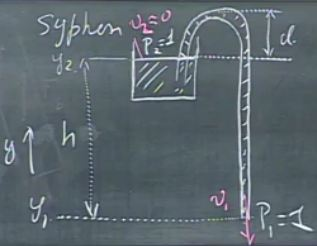
\includegraphics[scale=0.8]{\pIImages/lec28_siphon}
\end{center}

$v_2$, the velocity of the liquid in the container, can be approximated as zero, if it is much larger than the diameter of the hose.\\
Both the top of the liquid in the container and the liquid flowing out is directly exposed to the atmosphere, so $P_1 = P_2 = 1$ atm. Therefore, in our conservation of energy equation, we lose the pressure terms. With that in mind, having different $y$ values this time, and $v_2 \approx 0$, we find, also using $y_2 - y_1 = h$,

\begin{align}
\frac{1}{2} \rho v_1^2 + \rho g y_1 &= \rho g y_2\\
\rho v_1^2 &= 2 \rho g (y_2 - y_1)\\
v_1 &= \sqrt{2 g h}
\end{align}

This is \emph{exactly} the velocity we would find for an object being accelerated down by gravity. When starting at 0 velocity and having fallen a distance $h$, an object in free fall has the velocity $\sqrt{2 g h}$. In other words, the siphoned liquid is acting as if it's in free fall.

That much may be intuitive, but the strange part is once the flow has begun, we can raise the hose up, i.e. increase $d$, up until the $\approx \SI{10}{m}$ limit discussed earlier (for water), as long as the end of the hose is below the container, and the liquid will keep flowing.\\
We need to get it started manually, though, but sucking on the free end. Once that's done, the entire container will empty all by itself.

\subsection{A few quick experiments}

Consider a funnel, with a ping-pong ball inside:

\begin{center}
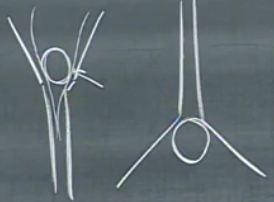
\includegraphics[scale=0.8]{\pIImages/lec28_funnel}
\end{center}

First, we hold it upright. If we try to blow and get the ball to move upwards, what will happen? The opposite of what we might think: the harder to blow, the more the ball is sucked down. According to the Bernoulli principle, the pressure is lower in the thin part, where the velocity is high. Therefore, there is an underpressure there, and the ball is sucked down more than it is blown upwards.

The effect is strong enough that we can do the experiment upside down, and hold it in place (for a short time, at least) merely by blowing out, as the second figure above shows.

Next, we have an air pump, blowing to keep a ping-pong ball floating in mid-air:

\begin{center}
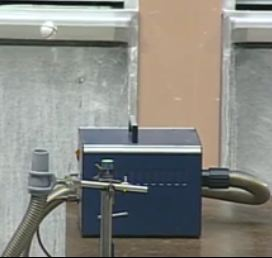
\includegraphics[scale=0.8]{\pIImages/lec28_air_pump}
\end{center}

It is held up for reasons to do with turbulence, which is more complex than we can discuss here. However, Bernoulli's principle comes into play in another way: the stability. While it's obviously difficult to show this in a still image, the ball wobbles back and forth, but never falls out. Even when the hose is tilted perhaps 10-20 degrees, the system is still stable. This stability is because of Bernoulli's principle.

\begin{center}
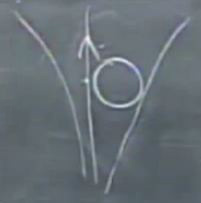
\includegraphics[scale=0.6]{\pIImages/lec28_divergence}
\end{center}

The air is blowing faster near the center, as it is diverging away (the area is becoming larger, so the velocity goes down, as we saw earlier).\\
Therefore, the pressure is the lowest near the center, and when the ball moves away, it is being sucked back in by the lower pressure.

Finally, the professor demonstrates what happens if you fill a glass half-way, put a piece of cardboard (or some paper similar to a postcard in thickness, perhaps) over the top, and then turn it upside down. The liquid will tend to stay in place even upside down, with no support, so not only is the paper is held up against gravity, the liquid is as well.\\
This happens because air pressure is acting to push the paper up, stronger than gravity is pulling the water down.\\
There are other things at play too, though, including surface tension. I have not been able to find a fully satisfactory explanation of this, even though it seems so simple.

For example, why does this not happen when you simply turn the glass upside down, without the paper? Clearly, the paper isn't increasing the air pressure; if the air pressure can support the liquid via the paper, it must obviously be able to support the liquid itself, too! So why does the water simply run out, as we would expect intuitively, but perhaps not expect considering air pressure?

The explanation appears to be quite a bit beyond this course, in Rayleigh-Taylor instability. If the water surface could be \emph{perfectly} flat, it appears that it would indeed not fall out, though achieving this in practice is clearly either extremely difficult or plain impossible.

%%% Local Variables:
%%% TeX-master: "../../main"
%%% End:


\chapter{Week 14}

\section{Lecture 30: Simple harmonic oscillations of suspended solid bodies}

The first half (or so) of this lecture is mostly a review of physical pendula. I will make the notes for that part rather brief, as it's easy to go back to previous chapters of these notes for a review.

We will make frequent use of a formula we derived in lecture 21 (and also derived here in lecture very quickly).

\begin{equation}
T = 2 \pi \sqrt{\frac{I_P}{b M g}}
\end{equation}

where $b$ is the distance between the point a pendulum is fixed, and its center of mass. This was derived for a rod, but holds for any geometry, as shown in this lecture. We will use it for rods, hula hoops, solid disks and simple pendula (a mass on a massless string) here. All we need to do is find $b$ and  $I_P$, the moment of inertia about the point where it is fixed (and therefore rotates); when that is done, we can easily calculate the period of that system.

\subsection{Rod}

For a rod, $I_{cm} = (1/12) M \ell^2$. The point P is then located a distance $b = (\ell/2)$ from the center of mass, as we rotate it about its end. Using the parallel axis theorem, $I_P = I_cm + M b^2 = (1/12) M \ell^2 + M \ell^2/4 = (1/3) M \ell^2$. Using those two equivalences,

\begin{equation}
T_{rod} = 2 \pi \sqrt{\frac{(1/3) M \ell^2}{(\ell/2) M g}} =  2 \pi \sqrt{\frac{2 \ell}{3g}}
\end{equation}

The lecture has a demonstration about several pendulum types, where each has a period of approximately 1 second. We want to know how long/large each type of pendulum should be to match that, so let's solve this for $\ell$ also:

\begin{equation}
\frac{3 g T_{rod}^2}{8\pi^2} = \ell
\end{equation}

For $T = \SI{1}{s}$, $\ell \approx 37.27$ cm, assuming we rotate it about the exact end.

\subsection{Simple pendulum}

Next, they ask how long a simple (``regular'') pendulum should be to have a period of 1 second. We use find the period of such a pendulum using the first equation above, using $b = \ell$ and $I_P = M \ell^2$. Doing so quickly gives you

\begin{equation}
T_{simple} = 2 \pi \sqrt{\frac{\ell}{g}}
\end{equation}

Again, let's solve for $\ell$.

\begin{equation}
\frac{g T_{simple}^2}{4 \pi^2} = \ell
\end{equation}

Here, we find a length of about $24.85$ cm.

\subsection{Ring}

We repeat the process for a ring, e.g. a hula hoop, where all the mass can be approximated to be at the circumference. Its center of mass will then be at the geometrical center, i.e. mid-air. Physics doesn't care, and we can use the same formula anyway. Quite amazing, really.\\
Here, we find a moment of inertia of $M R^2$ about the center of mass. Since point P is a distance $b = R$ away, we must add to that $M R^2$ from the parallel axis theorem, and find $I_P = 2 M R^2$.

\begin{equation}
T_{ring} = 2 \pi \sqrt{\frac{2 R}{g}}
\end{equation}

As the professor notes, this is exactly what you would find for a simple pendulum of length $\ell = 2 R$, i.e. with the same length as the diameter of the hula hoop. That makes it a bit unnecessary to solve for $R$, since we could just say that $R = \ell/2$, but I will do so anyway for completeness.

\begin{equation}
\frac{g T_{ring}^2}{8\pi^2} = R
\end{equation}

As expected, we find $R \approx 12.42$ cm, half (ignoring rounding) the length of the simple pendulum. 

\subsection{Solid disk}

Finally, we do this for a solid disk (solid except for a negligibly small hole where it's fixed, of course). Here, $I_{cm} = (1/2) M R^2$, and so adding $M R ^2$ for the parallel axis theorem gives us $(3/2) M R^2$.

\begin{equation}
T_{disk} = 2 \pi \sqrt{\frac{(3R}{2g}}
\end{equation}

Or, solved for $R$:

\begin{equation}
\frac{g T_{disk}^2}{6 \pi^2} = R
\end{equation}

$R \approx 16.56$ cm, or $d = 33.12$ cm, which is $4/3$ times that of the hollow ring.\\
The rod must also be exactly 50\% longer than the simple pendulum.

\subsection{Lecture question}

``Suppose we scale up the radius of our planet (keeping its mass density fixed), and the size and mass of a physical pendulum by a factor of 2. How will the period of oscillation change?''

Hmm... Many things will have to change, $g$ being one. Let's first find the change in Earth's mass, and then after that find the change in $g$, before we move on to the pendulum.

Even before that, the period of an ideal pendulum (which I chose from the various types as it's simple) is given by

\begin{equation}
T = 2 \pi \sqrt{\frac{\ell}{g}}
\end{equation}

For a uniform density, we have $M_{old} = (4/3) \rho \pi R^3$ and $M_{new} = (4/3) \rho \pi (2R)^3$, so the mass goes up by a factor of 8 from the $2^3$.\\
The distance to the center of the Earth also doubles, so $g$ changes not only due to the increased mass:

\begin{equation}
\frac{g_{new}}{g_{old}} = \frac{(8 GM)/(2R)^2}{(G M)/R^2} = \frac{8R^2}{(2R)^2} = 2
\end{equation}

So $g$ doubles. Since the period depends on $\ell/g$, which becomes $(2\ell)/(2g)$, the period is unchanged.

\subsection{Oscillating liquid in a U-tube}

Let's now move away from the fairly familiar territory above into something new: oscillating liquids.\\
We have a liquid in a U-shaped tube. The entire mass of the liquid is $M$, the density $\rho$ and the ``length'' of the liquid, at the center of the tube, is $\ell$.

The tube has a cross-sectional area $A$ everywhere along it.

\begin{center}
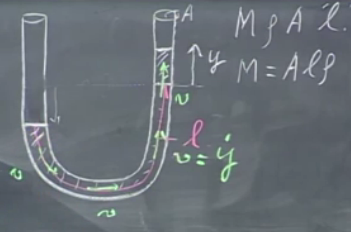
\includegraphics[scale=0.8]{\pIImages/lec30_utube}
\end{center}

As shown above, we displace the liquid so that it is at a height $y$ above equilibrium height on one side, and a height $y$ below at the other. We also denote the velocity of the liquid as $v = \dot{y}$, which is the same everywhere, at one instant.\\
Say we denote the equilibrium point as $U = 0$ for the system, where $U$ is the gravitational potential energy.\\
If we then displace some liquid as shown, say of mass $\Delta m$, the increase in gravitational potential energy is simply $\Delta m g y$, using $\Delta U = m g h$ with other variable names. This works because the same amount of liquid that is above equilibrium on the right side must be taken from the left side, and so it is equivalent to simply lifting that liquid up a distance $y$, regardless of which side this happens on.

There will be frictional losses and such in this system, but if we neglect that for a while, we can derive an approximate period of oscillation by using the conservation of mechanical energy.

In doing so, we find

\begin{equation}
\frac{1}{2} M (\dot{y}) + \Delta m g y = \text{constant}
\end{equation}

If we substitute in $M = A \ell \rho$ and $\Delta m = A y \rho$,

\begin{equation}
\frac{1}{2} A \ell \rho (\dot{y})^2 + A \rho g y^2 = \text{constant}
\end{equation}

If we take the time derivative, we will have a differential equation in $y$ which has $\ddot{y}$ as the highest derivative. Let's do that and see:

\begin{align}
\frac{1}{2} A \ell \rho 2 (\dot{y}) \ddot{y} + A \rho g 2 y \dot{y} &= 0\\
\ell \ddot{y} +  2 g y &= 0\\
\ddot{y} +  \frac{2 g}{\ell} y &= 0
\end{align}

Many things cancel, including $\dot{y}$. We get a result that is clearly a simple harmonic oscillation! However, more in this case than we have seen previously, this result is not that accurate; at least not for the demonstration in lecture. There is a lot of damping, i.e. the amplitude goes down from its maximum quickly, and as that happens, the period is affected.\\
Anyhow, we know the solution to this differential equation very well by now:

\begin{align}
y &= y_{max} \cos(\omega t + \varphi)\\
\omega &= \sqrt{\frac{2 g}{\ell}}\\
T_{tube} &= 2 \pi \sqrt{\frac{\ell}{2 g}}
\end{align}

This happens to be the same answers as you would find for a simple pendulum of length $\ell/2$ -- nature is funny that way.

Solved for $\ell$, since we did that for the rest,

\begin{equation}
\frac{g T_{tube}^2}{2 \pi^2} = \ell
\end{equation}

For $T = 1$ s, we need $\ell = 0.497$ m or about 50 cm.

\subsection{Torsional pendulum}

Nature really loves these simple harmonic oscillators. Granted, in many of these derivations we use a small angle approximation, but still.\\
For this one, we won't need to do that.

In a torsional pendulum, we can have for example an object hanging from a wire, which we rotate, and then let the wire's restoring torque try to get itself back to equilibrium.\\
Like a simple spring pendulum, a torsional pendulum has a period that is independent of the amplitude, assuming we don't permanently deform the wire, and stay in a region where the restoring torque can be considered linear with regard to the angle we twist the wire.

Consider this system:

\begin{center}
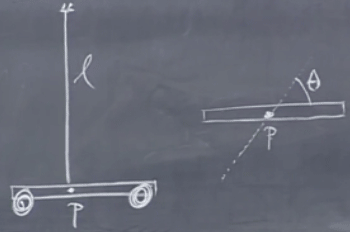
\includegraphics[scale=0.8]{\pIImages/lec30_torsional_pendulum}
\end{center}

(Left: as seen from the front; right: as seen from above, after giving the mass a small twist.)

The torque relative to point P is given by

\begin{equation}
\tau_P = -\kappa \theta
\end{equation}

where $\kappa$ (Greek letter kappa) is the \emph{torsional spring constant}. Just as with a spring oscillator, we have a minus sign to denote a restoring torque (or force, in that case), a spring constant, and something the torque/force is proportional to: here an angle, but in the case of a regular spring oscillator, a displacement.

Since the product $\kappa \theta$ must be in newton-meters, and $\theta$ is in radians, the units of $\kappa$ must be N m/rad (though radians are dimensionless, and perhaps we could say the units are already in N m, though that would be a bit confusing).

The torque is always equal to $I_P \alpha = I_P \ddot{\theta}$, so 

\begin{align}
- \kappa \theta &= I_P \ddot{\theta}\\
\ddot{\theta} + \frac{\kappa}{I_P} \theta &= 0
\end{align}

which is a simple harmonic oscillation -- without using any small angle approximation. As usual, the solution to this differential equation is

\begin{align}
\theta    &= \theta_{max} \cos(\omega t + \varphi)\\
\omega &= \sqrt{\frac{\kappa}{I_P}}\\
T          &= 2 \pi \sqrt{\frac{I_P}{\kappa}}
\end{align}

where $\omega$ is the angular frequency, a constant, not to be confused with $\dot{\theta}$ which is the angular velocity. The angular velocity varies with time; it is at a maximum at $\theta = 0$, and zero at $\theta = \theta_{max}$.

$\kappa$ is a function of the cross-sectional area, the length, and of course of the material in question. If the wire is thicker, $\kappa$ will go up, as we would expect; if you instead make it longer, $\kappa$ goes down.\\
Both are intuitive: a thick wire is much harder to turn than a thin one. Also, if you make it longer, it becomes easier to twist -- that also makes sense. A very short steel wire/rod is almost impossible to twist 10 degrees while grabbing each end of the wire/rod, but if it's very long, it's not a problem (unless it's also very thick, so that $\kappa$ is high for that reason).\\
Exactly how this is calculated is not shown, as it is a apparently more complex than the equivalent calculation for the linear case, using Young's modulus.

In the lecture demonstration, we have a 2.5 meter long piano wire, which is either 25/1000" or 1/25000" thick -- the subtitles say the latter, but I'm doubtful. It's a piano wire, which (according to Wikipedia) usually range from about 1/30 to 1/3 inches in diameter. Why would this one be a hundred times thinner?\\
In either case, the professor calculates $\kappa \approx 4 \times 10^{-4}$ Nm/rad for this wire.

If we now calculate the moment of inertia, we can predict the period of the pendulum.\\
We ignore the moment of inertia of the wire, since it's very thin, and has a near-zero moment of inertia about this rotation axis.

Here's a closeup of the part of the system with a non-negligible moment of inertia:

\begin{center}
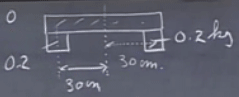
\includegraphics[scale=0.8]{\pIImages/lec30_torsional_pendulum2}
\end{center}

We can approximate the masses as point particles, each having a moment of inertia of $M R^2$ about the center axis (point P), so the total moment of inertia is approximately $I_P \approx 2 M R^2 = 2(\SI{0.2}{kg})(\SI{0.3}{m})^2 = \SI{0.036}{kg m^2}$.

Using the equation we found earlier, we find $T = \SI{59.608}{s} \approx \SI{60}{s}$.

The rest of the lecture is then demonstrations of this concept. The prediction is fairly accurate even for very large angles -- multiple rotations, not just some 30 degrees or such. The angular velocity is then very high (at times) for large angular displacements, since it must rotate much longer in the amount of time (since the period is independent of amplitude). As mentioned earlier, this is only true as long as we don't leave the region where Hooke's law is valid, and/or permanently deform the wire.

For half a period at 1 rotation, $T = 28.8$ s is measured. For three full rotations, half a period is measured as 28.5 seconds. For 10(!) full rotations, the period is measured as 29.2 seconds.\\
There is a reasonable amount of uncertainty in the measurements, as it's hard to define exactly when it stops rotating. Also, our calculations themselves were really approximations (e.g. the moment of inertia about the rotational axis).

\section{Lecture 31: Pendulums and springs}

We have talked considerably about springs in the past, but we will now add a new twist: instead of just setting a spring system off equilibrium and then leave it be, we apply a time-varying force at some fixed frequency that we choose -- which does not have to be the same frequency that the system would oscillate at on its own.

\begin{center}
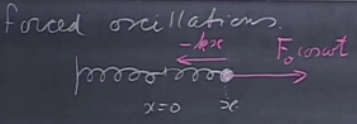
\includegraphics[scale=0.8]{\pIImages/lec31_forced}
\end{center}

An shown, we have a simple system with a mass $m$ connected to a spring. We drive it with some frequency $F_0 \cos (\omega t)$, where $F_0$ is the amplitude of the applied force.\\
We apply Newton's second law to the system, with $a = \ddot{x}$:

\begin{align}
m \ddot{x} &= - k x + F_0 \cos (\omega t)\\
\ddot{x} + \frac{k}{m} x &=  \frac{F_0}{m} \cos (\omega t)
\end{align}

Looks like a simple harmonic oscillator, except that the right-hand side is not zero, which of course changes things considerably.\\
In the beginning, the behavior can be fairly complex; we call this the transient phase, since it is indeed transient: it goes away after a while.\\
After the transient phase, we enter the \emph{steady state}. Here, the driver has ``won'', and the system oscillates at a steady frequency: that of the driver, so $\displaystyle f = \frac{\omega}{2 \pi}$ for the frequency (unless you prefer the angular frequency $\omega$ as-is). The mass will then move as described by $x = A \cos (\omega t)$, once the transient phase is over. The amplitude $A$ of this oscillation is not known, so let's try to find it.

The derivatives of this trial solution are (since we need $\ddot{x}$):

\begin{align}
x            &= A \cos (\omega t)\\
\dot{x}   &= -A \omega \sin(\omega t)\\
\ddot{x} &= -A \omega^2 \cos(\omega t)
\end{align}

We can then try to substitute $x$ and $\ddot{x}$ above into the differential equation we found earlier.

\begin{align}
-A \omega^2 \cos(\omega t) + \frac{k}{m} A \cos (\omega t) &=  \frac{F_0}{m} \cos (\omega t)\\
A\left(\frac{k}{m} - \omega^2\right)  &=  \frac{F_0}{m}\\
A\left(\omega_0^2 - \omega^2\right)  &=  \frac{F_0}{m}\\
A &=  \frac{F_0}{m\left(\omega_0^2 - \omega^2\right)}
\end{align}

Here, we have used $\displaystyle \omega_0 = \sqrt{\frac{k}{m}}$, which we call the natural frequency of the system. It is the $\omega$ we have seen before in spring systems -- the one it oscillates with naturally, if you offset it from equilibrium and then let it be. We add a subscript 0 to denote this, since $\omega$ is now the driving frequency.

Let's look at some limiting cases. In the case $\omega \ll \omega_0$; in that case, we find $A = F_0/k$.\\
If $\omega \gg \omega_0$, the amplitude goes to 0. (That it also becomes negative is something we will discuss shortly.)

If $\omega \to \omega_0$, i.e. we drive it at the natural frequency, the denominator goes to zero, and the amplitude goes to infinity. It doesn't go to infinity it practice, of course, but the amplitude does tend to become very large. We call this \emph{resonance}.\\
Frictional forces etc. limit the actual amplitude in practice.

If we plot the amplitude $A$ versus the driving (angular) frequency $\omega$, we find something like this:

\begin{center}
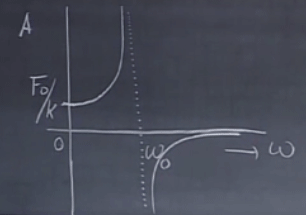
\includegraphics[scale=0.8]{\pIImages/lec31_amplitude}
\end{center}

The negative values mean that the object is now 180 degrees out of phase with the driver, which we don't go into any detail about in this lecture.

If we take a more realistic case (where the amplitude stays finite), and also plot the absolute value of the amplitude to get rid of the discontinuity of the phase shift, we get something like this:

\begin{center}
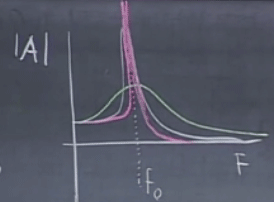
\includegraphics[scale=0.8]{\pIImages/lec31_amplitude2}
\end{center}

The less damping there is, the narrower the resonance peak is (shown in pink). With lots of damping, the peak becomes just a small bump (in green).

If we have a more complex system with more than 1 mass, all joined together with springs, we find the same number of resonance frequencies as there are masses, so a plot of amplitude vs driving frequency would have multiple peaks.\\
We can take this to the extreme, and consider a practically infinite number of such oscillators, in for example a violin string. We can think of each atom being a mass, connected to the others via a ``spring'' (in reality via electromagnetic forces).

In the case we have looked at earlier, we have a case of longitudinal oscillations: the objects move in the same direction as the spring, so to speak.\\
Oscillations/waves can also be transverse; electromagnetic waves are transverse, for example. Water waves are not good as an example, as they are a combination; in a fully transverse water wave, each molecule of water would simply move up and down, as the wave passes from side to side.

Sound is a longitudinal wave; at least in air, there appears to be some discussion about whether transverse waves in other media can be considered sound or not.

\subsection{Harmonics}

Let's look now at the example of shaking a string. As mentioned earlier, there will be many, many resonance frequencies. Consider the first few:

\begin{center}
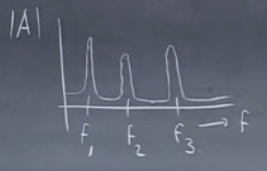
\includegraphics[scale=0.8]{\pIImages/lec31_harmonics}
\end{center}

We start off by shaking the string up and down at a low frequency, which we slowly increase. At one point, we will hit the first resonance frequency, also known as the first harmonic, or the fundamental. We denote this frequency as $f_1$.\\
At that point, the amplitude will be much greater than it was just before, and we will have a \emph{standing wave}. Each point of the curve will bob up and down, but that is all that happens. The movement is the greatest at the center, and zero at the two ends where the string is held.\\
Points where the string is standing still are called \emph{nodes} (while points of maximum amplitude are called \emph{antinodes}).

If we keep increasing the frequency, we will eventually find the second resonance frequency, or second harmonic, $f_2$. There will now be a node at the center of the string, while there will be two antinodes, evenly spaced. The two antinodes will be 180 degrees out of phase, so when one is at its highest point, the other is at its lowest.

Increase the frequency further, we find the third harmonic, $f_3$. This adds another node, so there are now two nodes and three antinodes.\\
Animated graphics are extremely useful here, so I suggest looking some up. Wikipedia has one on the page ``Node (physics)'' and several more in the article ``Vibrating string'', which shows the first five harmonics.

Here is a still image from the lecture, which is about the best I can do in these notes (in the lecture, Prof. Lewin also did a demonstration):

\begin{center}
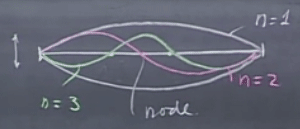
\includegraphics[scale=0.8]{\pIImages/lec31_nodes}
\end{center}

The first harmonic, $n=1$ (in white) just has the string being either all high, all low, or in transition between the two states.\\
The second harmonic, $n=2$ (in pink) has a node at the center, with the antinodes out of phase.\\
The third harmonic, $n=3$ (in green) has two nodes, with the leftmost and rightmost antinodes in phase with each other, and out of phase with the middle antinode.

These frequencies follow a simple relationship of $f_n = n f_1$, i.e. they are integer multiples of the fundamental frequency. If $f_1 = 100$ Hz, then $f_2 = 200 Hz$, $f_3 = 300 Hz$ etc.\\
In musical instruments, the second harmonic is therefore one octave higher than the first. The third harmonic is not one octave higher than the second harmonic, though, but rather an interval of a perfect fifth above.\footnote{In just intonation, a perfect fifth has a frequency ratio of 3:2, i.e. 1.5 times; in equal temperament, which most instruments use in modern times, a perfect fifth is exactly $2^{7/12} \approx 1.4983$ times the frequency of a given note, but this is now really becoming music theory.}  (An octave doubles the frequency, which would be 400 Hz, so the fourth harmonic in an octave above the second.)

The frequency of the fundamental/first harmonic depends on the string's mass, length and tension (or, if you prefer, the mass per unit length, length and tension).

Many musical instruments are of course stringed instruments. In the case of a piano, the strings vary in all three attributes.\\
In a violin, there are four strings, of essentially equal length. The thickness (and therefore mass per unit length) varies. Tuning is set by adjusting the tension in each string individually.\\
A higher tension causes a higher pitch, while a \emph{shorter} string causes a higher pitch (for a given tension and mass).\\
When playing a violin, the player changes the pitch by shortening the strings. When you fret a note (i.e. hold a string down against the violin's neck), the effective length that vibrates is shortened, and so the pitch goes up.

In the case we looked at earlier, with the driven spring and the long shaken string, the driver alone decided the frequency. How does that work in the case of e.g. a violin?\\
When we use a bow on a violin, that rubbing motion can be thought to consist of many, many different frequencies at which the string is ``driven''. The string picks out its resonance frequencies, and so the frequencies we hear are mostly the different harmonics, i.e. integer multiples of the string's fundamental frequency.

The ratio of the amplitudes of the different harmonics is what gives an instrument its \emph{timbre}. Consider a theoretical violin string that only oscillated at a single frequency $f_1$. The sound it would make is a pure sine wave -- which sounds like a very boring ``beep'' and nothing at all like a violin.\\
For a middle A note, both a violin and a piano produce a 440 Hz sound with several harmonics, but they sound very different, as the harmonic content of the two are very different.\\
Adding up only the odd harmonics -- 1, 3, 5 etc -- will produce a square wave, which adding up all harmonics gives a sawtooth wave. These terms are mostly used in synthesis of sound, but are also useful for describing the sound of real-world instruments. Violins have a lot of harmonic content, and are much closer to a sawtooth-shaped waveform than to a square-shaped one in timbre.

\subsection{Woodwind instruments}

Consider an overly simple woodwind instrument: a closed box of length $L$, filled with air, and a loudspeaker at the end that can generate different frequencies. We can find several such resonant frequencies, however, this time it's not the material itself that resonates, but rather the air inside it.\\
The air acts a bit like a spring if you excite it at the right frequencies. The harmonics are easily calculated as

\begin{equation}
f_n = \frac{n v}{2 L}
\end{equation}
where $n$ is the harmonic number, $v$ is the speed of sound in air (about 340 m/s) and $L$ is the length of the box.

This instrument isn't very practical though; it's not only closed, so that the sound will barely be audible outside, but it is driven by a loudspeaker. We can take care of that by opening up either one side, or both. What is now interesting (and rather strange, in my opinion) is that if we open up both sides of this box, and again put the loudspeaker at one end, we can still find the exact same resonance frequencies as we did before!\\
This would be referred to as an open-open instrument. Flutes are open-open (more or less).
We can also open up only one side, to create a closed-open instrument, such as a clarinet. In this case, the formula above doesn't apply; there is no additional detail to how or why it is different, though.

In reality, the loudspeaker is of course replaced by the player (or the player's mouth, rather).

\subsection{Other resonances}

Next, there is some talk about how everything has a resonance frequency: from car keys to frying pans and refrigerators, people and wine glasses.\\
The wine glass is demonstrated: by moving a clean, wet finger around the top of a wine glass, you can generate a fairly loud sound. What happens is just as with the violin string, our rubbing causes a ton of different frequencies to be generated, and the glass ``picks out'' its resonance frequency/frequencies and hums along at those.

Resonances can also be destructive. By playing back a tone that corresponds to the glass' fundamental resonance frequency at a loud volume, we can make the amplitude of oscillation so great that the glass breaks. This is demonstrated using a strobe light setup to allow us to see the deformations in the glass (which are about 470 Hz, which of course is far too fast to see otherwise).

Another well-known and oft-cited example is the Tacoma Narrows Bridge, first opened on July 1, 1940. It collapsed barely more than 4 months later, on a day of strong wind. However, while this is often presented as a resonance phenomena, it appears opinion has changed, and it is now consider to be due to aerodynamic flutter rather than forced oscillation. This is the same phenomena that causes a paper to oscillate when held steadily in constant airflow. Some also present it as a combination of multiple phenomena, and I certainly don't have the expertise to say who is correct, so I'll leave it at that.

Finally, the professor demonstrates what happens when the speed of sound in a medium changes -- or when the medium itself changes, rather, by filling his lungs with helium while speaking. Sound travels about 2.7 times faster in helium than in air, and so the pitch created by our vocal chords goes way up if your lungs are filled with helium rather than air.\\
Since helium is, well, helium, which doesn't contain the $\approx 20$\% oxygen we need to live, this experiment is dangerous if done incorrectly (or for anything but a short period of time).

\section{Lecture 32: Thermal expansion}

We begin the lecture by introducing the concept of thermometric properties. A thermometric property is a property of an object that depends on the object's temperature. A typical one, that we will look at in this lecture, is that many objects expand when heated, and contract when cooled.\\
If we heat up a gas in a closed container, the pressure in the container goes up, which is a thermometric property. If we heat an electric conductor, the electric resistance will tend to go up.\\
(That is why regular light bulbs often break when turned on; the current through them is at a maximum the first split second before it starts to reach its operating temperature (which happens extremely quickly). After that, the resistance goes up, and so the current goes down, to its steady state level.)

If we heat a metal bar, it will expand. Cool it, and it will shrink. If we bring a hot and a cold iron bar together, there will be heat transfer between the objects until they are in thermal equilibrium, i.e. when their temperatures are equal. Until then, the two bars will both change in size as their temperature changes.

We can construct a simple thermometer this way. We have a bar of some length $L$ of a known material, at a known temperature. We put the bar in melting ice, and measure a length $L_1$; we then put it in boiling water, and find a length $L_2$. We can then define a temperature scale such that, for example, $L_1$ means the temperature is 0 degrees, and $L_2$ means 100 degrees. This is basically how the Celsius scale works.\\
This scale is (or was) often called \emph{centigrade} (from Latin's centum, meaning hundred and gradus meaning step), though that name was formally obsoleted in 1948, and the scale is now known as the Celsius scale, after Anders Celsius, the Swedish astronomer who came up with it.\footnote{Apparently, his original scale was the opposite: ice melted at 100 degrees, while water boiled at 0. Carl von Linn\'e, also know as Carl Linnaeus, reversed the scale soon after Celsius' death.}

Another common temperature scale is the Fahrenheit scale, invented by German scientist Daniel Gabriel Fahrenheit. He used brine, a mixture of salt and ice, as the zero degree definition, and human body temperature as 100... roughly speaking, as 98.6 F is the most commonly quoted number for human body temperature these days, and 100 F is defined as having a fever.

Conversion between the two scale is relatively straightforward. 0 degrees C is 32 degrees F, while 100 degrees C is 212 degrees F. To convert, we use

\begin{align}
T_F &= \frac{9}{5} T_C + 32\\
T_C &= \frac{5}{9} \left(T_F - 32\right)
\end{align}

The two scales ``cross over'' at -40 degrees, so $\SI{-40}{{}^\circ\text{F}} = \SI{-40}{\degreeCelsius}$.

The third temperature scale (or perhaps rather unit) that is fairly common, especially very common in science, is the kelvin, which is an absolute temperature scale. Because it is absolute (see below), we do not talk about ``degrees'' kelvin, but just kelvin (just as we don't talk about degrees pascal).
The coldest temperature with any physical meaning, absolute zero, is by definition 0 K. At this temperature, it is often said that all motion stops (which is not entirely true, due to to the world of quantum mechanics), and so colder temperatures are not very meaningful. This might be expanded upon as early as next week, when Heisenberg's uncertainty principle is introduced.

The kelvin scale is closely related to the Celsius scale: it is offset by exactly 273.15 degrees C, so that 0 K = $\SI{-273.15}{\degreeCelsius}$. Therefore, water boils at 373.15 K (at 1 atm of pressure).

\subsection{Thermal expansion}

We can now get to the focus of this lecture: thermal expansion.\\
Say we start with a rod of length $L$. We heat it up by $\Delta T$ degrees C (or kelvin), and it gets longer by an amount $\Delta L$. We can approximate this amount in a simple way:

\begin{equation}
\Delta L = \alpha L \Delta T
\end{equation}

where $\alpha$ is known as the \emph{linear expansion coefficient}, with units of 1 over degrees Celsius ($1/{}^\circ$C).

As the values of $\alpha$ are often small, we can write them in terms of $10^{-6}/{}^\circ$C, equivalent to $\text{ppm/}^\circ$C or ppm/K.\\
$\alpha$ for a few common materials is

\begin{center}
\begin{tabular}{|r|l|}
\hline
$\alpha$ & ppm/${}^\circ$C\\ \hline
Copper & 17\\\
Brass & 19\\
Pyrex & 3.3\\
Invar & 0.9\\
Steel & 12\\
\hline
\end{tabular}
\end{center}

Invar is an alloy often used for its unusually low thermal expansion coefficient. There are several variations; the one usually called invar is 64\% iron and 36\% nickel. It was invented by Swiss scientist Charles \'{E}douard Guillaume in 1896; the invention won him the Nobel prize in physics in 1920.\\
Having a material with a low thermal expansion coefficient is important for many precision instruments, for example.

Consider a steel railroad track, 1000 meters long. In many climates, it might need to be usable at -15 degrees C, a cold winter's day, and also at +35, a hot summer's day, so $\Delta T = 50$ degrees. Using the formula above, and the value of $\alpha$ of steel, we find $\Delta L = 0.6$ meters. If the rail is continuous and can't expand in the ``forward'' direction, it will start to bulge either sideways or upwards, whichever is easier.

How is this taken care of? The rail needs to be able to expand, or it will deform and become unusable. One solution is very simple: the railroad has gaps in it. We need gaps of up to 60 cm per km, so for example 5 cm per 80 meters gives the rail space to expand. With large enough wheels, this causes a ``clunk'' when riding over it, but nothing more.

The professor then demonstrates the expansion of a brass bar, by using an ``amplifier'' device to turn the small (millimeter-scale) expansion into something more clearly visible (a large change in the angle of an indicator).

\subsection{Bimetals}

Bimetals are a very useful type of material. We take two metals with different linear expansion coefficients, and put them together (perhaps using welding):

\begin{center}
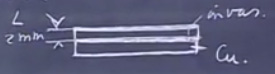
\includegraphics[scale=0.8]{\pIImages/lec32_bimetal}
\end{center}

When we heat this system, what happens? The copper must get longer, but the change in the invar's length is much less. Since we join them such that one can not expand without affecting the other, it will bend upwards, so that the invar is on the inside of an arc, and the copper is along the (longer!) outside. The difference in the length change of the two materials is

\begin{equation}
\Delta L_{Cu} - \Delta L_{invar} = (\alpha_{Cu} - \alpha_{invar}) L \Delta T
\end{equation}

For a 10 cm rod composed of copper and invar, the difference in expanded length is about 0.16 mm. However, the difference in height between the two sides will be about 3-4 mm\footnote{The professor says about 4 mm; a scientific paper on bimetal thermostats has a formula that gives about 3 mm; one or both are probably estimates, though.}, despite the small difference in length.

We can use bimetals for example in thermostats, so that a bimetal being sufficiently cold makes contact in an electric circuit, to turn a heater on. Once the bimetal is warm enough, it expands and ``bends away'', so that the contact is broken, and the heater turns off.

They can also be used for safety devices. Gas stoves sometimes use a ``pilot light'', basically a small flame, that is used to light the main burners. If the pilot light is off, but the gas is on, the room will fill up with a flammable and explosive gas, which can of course cause horrible accidents. One of several ways to prevent this is to use a bimetal, such that the gas supply is only on as long as the pilot light is burning. When it goes out, the bimetal cools down, and in some way automatically turns off the gas supply.

We can build thermometers of bimetals. We could have a construction like this:

\begin{center}
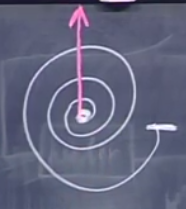
\includegraphics[scale=0.8]{\pIImages/lec32_bimetal_thermometer}
\end{center}

The outer end is attached to some casing and cannot move. The pink arrow is some form of indicator, attached at the center.\\
When the bimetal is heated, it will try to curl up even tighter than it already is, and the arrow moves clockwise. When the bimetal is cooled, the arrow moves towards the left. All we need, then, is to calculate how much it will turn, and then add a temperature scale around this.

Here is such a thermometer:

\begin{center}
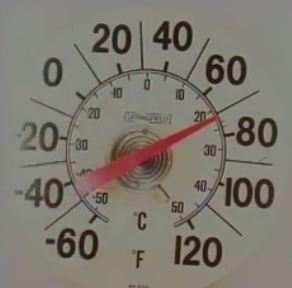
\includegraphics[scale=0.8]{\pIImages/lec32_bimetal_thermometer2}
\end{center}

\subsection{Volumetric expansion}

Let's now consider how much the \emph{volume} of an object increases when heated.\\
For simplicity, we use a cube, of side $L$. We increase the temperature by $\Delta T$.

The old volume is $V = L^3$, and the new volume $V + \Delta V = \left(L + \Delta L\right)^3$. Let's try to approximate this for a small increase in $L$.

\begin{align}
\Delta V &= \left(L + \Delta L\right)^3 - V\\
\Delta V &= L^3 \left(1 +  \frac{\Delta L}{L}\right)^3 - L^3
\end{align}

Here, we simply factor out $L^3$, and then also substitute $V = L^3$.\\
Next, we use the first-order term of the Taylor expansion of $(1 + x)^n \approx 1 + n x$, where $x = \Delta L/L$ and $n = 3$:

\begin{align}
\Delta V &= L^3 (1 + 3 \frac{\Delta L}{L})     - L^3\\
\Delta V &= 3 \frac{L^3 \Delta L}{L}\\
\Delta V &= 3 L^2 (L \alpha \Delta T) \label{eq:lec32eq3}\\
\Delta V &= 3 \alpha L^3  \Delta T\\
\Delta V &= 3 \alpha V  \Delta T
\end{align}

In \eqref{eq:lec32eq3} we simply substitute $\Delta L = L \alpha \Delta T$.\\
We find, then, that the result depends on some value $3 \alpha$. We usually write this as $\beta = 3 \alpha$, and call it the \emph{cubic expansion coefficient} (or volumetric expansion coefficient).

The reason we can use the linear term only is that the next term in the Taylor series contains $\alpha^2$, which is extremely small. (For $L = 1$ m, $\Delta T = 100$ K and $\alpha = 10^{-5}/{}^\circ$C, the quadratic term is $3 \times 10^{-6}$, versus $1.003$ for the two terms we do have. )The higher-order terms are much smaller yet.

We can now look at how a(nother) simple thermometer can work, e.g. a mercury thermometer, though other fluids are used these days, for safety reasons.\\
Mercury has a $\beta$ of about $18 \times 10^{-5}/{}^\circ$C, while Pyrex has a value of roughly $\num{1e-5}$ (3 times the value of $\alpha$ we had earlier). A Pyrex container with mercury inside will then barely expand when heated, but the mercury inside certainly will -- about 18 times as much. If we make a reservoir of mercury at the bottom, and then a very narrow column upwards, we get this:

\begin{center}
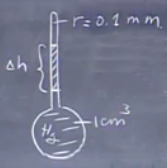
\includegraphics[scale=0.8]{\pIImages/lec32_mercury_thermometer}
\end{center}

When the mercury/liquid expands, it has nowhere to go except up the display tube. We calculate how much the column will grow per degree, and create the scale accordingly. All that remains is then to fill it up to the correct level, and nature takes care of the rest.

Consider a tiny radius of 0.1 mm, as shown, for the display tube. Ignoring the expansion of the Pyrex (which we probably shouldn't do if we actually built this), if our 1 cubic centimeter of mercury/liquid goes up in temperature by 10 degrees C, it expands by $V \beta \Delta T = \SI{0.0018}{cm^3}$.\\
A very small increase, but hold on. A height $h$ in the tube can hold a volume $\pi r^2 h$, so we find $\displaystyle h = \frac{\SI{0.0018}{cm^3}}{\pi (\SI{0.01}{cm})^2} = 5.73$ cm! That gives us almost 6 mm per degree, which is quite a bit more than most such thermometers I've seen; very easily readable.

\subsection{Expansion of water}

Water is a peculiar substance. We have so far only talked about substances that expand when heated, but water behaves rather differently at some temperatures.\\
If we take room-temperature water and cool it down slightly, it shrinks, as expected. However, once we reach 4 degrees C, cooling it \emph{further} down to 0 will cause the water to expand!\\
Put in other words, the density of water is at a \emph{maximum} when it is at 4 degrees C. This also implies that in this region between 0 and 4 degrees C, $\beta < 0$, so it changes sign at 4 degrees C.

This causes several important phenomena. For one, the 4 degree water sinks to the bottom, while ice tends to float; therefore, the bottom of lakes and such tend to remain liquid all year round, so that fish can survive below the ice.

For most materials, the solid of a material tends to sink in its liquid (i.e. the solid tends to have a higher density, so that a given amount, measured by mass, is more compact), but water is an exception.


\section{Lecture 33: Ideal gas law}

While liquids are almost entirely incompressible, as we have seen, gases are not. In a liquid, the molecules are still moving around (as opposed to a solid), but are quite closely packed, at least compared to a gas. In a gas, there is a fairly large distances between molecules, unless the pressure is very high. Therefore, we can compress gases rather easily, until the molecules become about as closely packed as in a liquid. If we keep compressing a gas at that point, it may undergo a phase change, usually to a liquid, but this depends on the compound. Carbon dioxide is perhaps the most well-known compound to only exist in gas and solid phases at atmospheric pressures; the liquid phase only exists at higher pressures (higher than about 5.1 atmospheres), so it either \emph{deposits} (goes from gas directly to solid) or \emph{sublimes} (also known as sublimates), meaning it goes from solid directly to gas.\\
Air at 1 atmosphere has a density 1/1000 times that of water; that says something about the relative distances between molecules involved.

Here are some definitions we'll soon use, from a lecture supplement sheet:

\begin{center}
\begin{tabular}{|r|l|l|}
\hline
Symbol & Meaning & Unit/value\\ \hline
P & Pressure & Pascal ($\text{N/m}^2$)\\
V & Volume & $\text{m}^3$\\
T & Temperature & Kelvin (K)\\
N & Number of molecules & \\
n & Number of moles (see below) & mol\\
$\text{N}_\text{A}$ & Avogadro's constant & $6.022 \times 10^{23} \text{mol}^{-1}$ \\
R & Universal gas constant & \SI{8.31}{J/(K mol)}\\
k & Boltzmann constant & $R/N_A = \SI{1.38e-23}{J/K}$\\
Z & number of protons in a nucleus & \\
N &  number of neutrons in a nucleus & \\
A & atomic number, $A = Z + N$ & \\ \hline
\end{tabular}
\end{center}

We will use the unit of a \emph{mole}, which is a unit not unlike terms like a dozen, only way larger. 1 mol is defined as the number of atoms in 12 grams of carbon-12; 1 mol of water means approximately $6.022 \times 10^{23}$ molecules of water, for example. The unit can be used for anything. 1 mol of eggs is a lot; something like $10^{12}$ eggs were produced in 2002, so 1 mol of eggs would, at that rate, take 602 214 129 000 years to produce! Nevertheless, it is not much more than a number -- only that it has a unit attached to it. I think I'll stick to dozens as far as eggs go.

Note that moles are about a number of something, but not \emph{necessarily} number of \emph{atoms}. One mole of helium molecules is the same as one mole of helium atoms, since helium doesn't tend to group into molecules at all.\\
On the other hand, one mole of oxygen gas ($O_2$) contains 2 moles of oxygen atoms. Unless specified otherwise, one mole will here refer to the molecular count, so that 1 mole of carbon dioxide and 1 mole of helium has the same number of molecules, but \emph{not} the same number of individual atoms.

\subsection{Ideal gas law}

The \emph{ideal gas law} states that

\begin{equation}
P V = n R T
\end{equation}

using the definitions we introduced above. Both sides of this equation have the dimension of energy, i.e. units of joules using the MKS units. $P V$ has units of $(\text{N/m}^2)(\text{m}^3) = \text{N m} = \text{J}$, while $n R T$ has units of $(\text{mol})(\text{J/(K mol)})(\text{K}) = \text{J}$.

Using the Boltzmann constant $k = R/N_A \approx \SI{1.38e-23}{J/K}$ that we listed in the table above, we can also write the ideal gas law as

\begin{equation}
P V = N k T
\end{equation}

where $N$ is now a dimensionless number relating the number of molecules (not in moles, but the actual number), $k$ is the Boltzmann constant as in the table above, and the rest of the variables remain as they were.

Before we use the ideal gas law, we'll have a quick look at atomic number and related things.\\
An atom has $Z$ protons (that define which element it is), $N$ neutrons (which define the isotope) and, if it is electrically neutral (i.e. not an ion), also $Z$ electrons to balance out the change. (As we learn in 8.02 if not in high school, the proton and the electron have exactly the same magnitude of change, only opposite signs.)\\
The \emph{atomic mass number} $A$ is then simply $A = Z + N$, and defines how many protons plus neutrons there are in the nucleus.\\
Protons and neutrons have very close to the same mass (they differ by about 0.14\%), while is this context, electrons have almost zero mass (an electron only has 0.05\% of a proton's mass) that we can often neglect.

Let's look at carbon as an example. Carbon has 6 protons (6 protons defines the element, so anything else wouldn't be carbon). Carbon-12 also has 6 neutrons, so $A = 12$, which is also what we specify in its name.\\
Other forms of carbon have differing number of neutrons; known isotopes range from carbon-8 (2 neutrons) to carbon-22 (16 neutrons), though most of these are highly unstable. Only carbon-12 and carbon-13 are stable; carbon-14 has a half-life of 5730 years and is commonly used for radiometric dating of organic things.

As shown in the definition above, 1 mol of carbon-12 has a mass of 12 grams exactly. 1 mol of carbon-14 has a mass of approximately 14 grams (the approximate mass of 1 mol, in grams, of any atom is simply the number of nucleons), though because of the small difference in mass between protons and neutrons, the actual mass is closer to 14.00324 g.

Another example would be that of oxygen gas; it has a \emph{molar mass} of about 32 g/mol. Each oxygen atom has 8 protons and 8 neutrons (some oxygen atoms are oxygen-17 and oxygen-18, but the vast majority are oxygen-16, so the average atomic mass number is about 16). Each $O_2$ molecule consists of two oxygen atoms, so we find $2 \times (8 + 8) = 32$ g/mol.

Since the mass of a proton and a neutron is almost equal, we can to a reasonable approximation write the mass of a molecule as $m_{molecule} = A \times \SI{1.67e-27}{kg}$, where the mass of a proton is $m_p \approx \SI{1.672621e-27}{kg}$.

\subsection{Ideal gas law example}

The ideal gas law is an approximation, but one that holds reasonably well for most gases. Therefore, we don't need to specify what the gas is to use it.

Say we have a gas at 1 atmosphere, so $P \approx \SI{1.03e5}{Pa}$. We also have $n = \SI{1}{mol}$ of the substance. We do this at room temperature, so $T = \SI{293}{K}$.

$P V = n R T$, and we know everything except $V$. ($R$ is a constant, so we know that, too.)\\
We solve for $V$, and find

\begin{equation}
V = \frac{n R T}{P} = \frac{(\SI{1}{mol})(\SI{8.31}{J/(K mol)})(\SI{293}{K})}{\SI{1.03e5}{Pa}} \approx \SI{0.0236}{m^3} \approx \SI{23.6}{L}
\end{equation}

So this is (approximately) true whether the gas is helium, oxygen, nitrogen etc., as long as there is 1 atm of pressure. Of course, this only holds as long as the substance in question would actually \emph{be} a gas as this temperature and pressure. If we try to use water at 1 atmosphere and room temperature, then our results will be nonsense; we still find almost 24 liters, but the correct answer is about 18 mL, so this ``estimate'' is over 1000 times too high. (It also doesn't hold very well for water vapor either, because water molecules are fairly attracted to each other, which makes the ideal gas law not hold.)\\
We will soon look at phase diagrams, which will help us figure out whether a substance will be a gas, liquid or solid (or a mixture of two or three of these) at a given temperature--pressure combination.

As the name implies, the law is exactly true for \emph{ideal} gases (by definition: an ideal gas is one that obeys this law). Many real gases are close to ideal under common circumstances, though. 1 mole of oxygen at atmospheric pressure and room temperature is within 0.1\% of what the ideal gas law predicts (the true value is smaller than the approximation). At 20 atmospheres, the result is about 2\% off, still with the correct result being smaller than the approximation.

\subsection{Ideal gas law with different molar mass gases}

Consider the case when we have two gases where the molar masses are very different, but we have the same number of moles of each gas. Both are at room temperature, and they are in identical containers. $n$, $T$ and $V$ are the same, and via the ideal as law, that means $P$ is also the same. The masses of the molecules are very different however, and since we have the same amount, the total mass of one gas must also be much greater than the mass of the other.

The molecules in the gas are flying around in all directions, with different speeds. We consider an average speed $\overbar{v}$ for simplicity.\\
Say a molecule of mass $m$ hits the container wall with speed $\overbar{v}$. It bounces back in an elastic collision, which implies a momentum change of $2 m \overbar{v}$ in magnitude -- its forward momentum is replaced with backwards momentum of the same magnitude.

That is just the momentum change of one molecule, though. We want the rate of momentum transfer over time.

If we consider a cube of side $L$, it takes a molecule a time $t = \dfrac{2 L}{v}$ to come back to a wall after bouncing off it, in the simple case where it moves in one dimension only. Therefore, the rate of momentum transfer (per second) is $\dfrac{2 m v}{t} = \dfrac{2 m v}{\frac{2 L}{v}} = \frac{m v^2}{L}$. (Thanks to Grove for this derivation.)

The rate of momentum transfer for the entire system is therefore proportional to $m v^2$. Rate of momentum transfer is force, and force is proportional to pressure. It certainly looks as if $m \propto P$ -- which the ideal gas law clearly says is not the case!\\
The only way this works out, and how it actually does work, is if $m v^2$ is constant for a given temperature, i.e. it is independent of $m$! In other words, the speed of the particle is such that it balances out its mass; the smaller the mass, the larger the speed, and vice versa.

For example, comparing helium and oxygen gas, we can write that

\begin{equation}
m_{He} \overbar{v_{He}}^2 = m_{O_2} \overbar{v_{O_2}}^2
\end{equation}
\begin{equation}
\overbar{v_{He}} = \sqrt{\frac{m_{O_2}}{m_{He}}}\ \overbar{v_{O_2}}
\end{equation}

Oxygen molecules have an average speed of about 480 m/s at room temperature. Since the ratio of masses here is about 8, helium molecules move, on average, about $\sqrt{8} \approx 2.82$ times faster than oxygen molecules, which is about 1350 m/s.\\
If we mix the two cases, the only way the ideal gas law can hold is if these speeds still stay true, so that the lighter molecules move faster.

\subsection{Ideal gas law example \#2}

``A closed container with a volume of $\SI{8000}{cm^3}$ is filled with Xenon gas. The gas temperature is 273 K (the container is placed in ice water) and the pressure is 2.0 atm.

How many moles of Xenon are in the container?''

Well, we use $P V = n R T$. We want $n$, so

\begin{equation}
n = \frac{PV}{RT} = \frac{(2\times\SI{1.03e5}{Pa})(\SI{0.008}{m^3})}{(\SI{8.31}{J/(K mol)})(\SI{273}{K})} \approx \SI{0.726}{mol}
\end{equation}

``The container is now submerged in boiling water until the gas inside the container is at 373 K. You may assume that the increase in volume of the container is negligible.

What is the pressure of the xenon?''

We re-rearrange the equation to give
\begin{equation}
P = \frac{n R T}{V}
\end{equation}

Plugging in the given numbers, plus the $n$ we found above,

\begin{equation}
P = \frac{n R T}{V} = \frac{ (\SI{0.726}{mol})(\SI{8.31}{J/(K mol)})(\SI{373}{K})}{\SI{0.008}{m^3}} \approx \SI{281300}{Pa} = \SI{2.7}{atm}
\end{equation}

\subsection{Phase diagrams}

We will now look at phase diagrams. The \emph{phase} of a substance is basically whether it is a solid, liquid or a gas; however, phase and state of matter are not the same thing. For example, while all water ice is solid (its state of matter), there are many different phases. Ice Ih is by far the most common water ice; Ice Ic essentially the only other form naturally occurring on Earth. Over a dozen other forms of water ice have been created in labs, by varying the temperatures and pressures.\\
I will mostly (perhaps entirely) use phase and state of matter interchangeably in the rest of these notes.

Here's a simple, general phase diagram:

\begin{center}
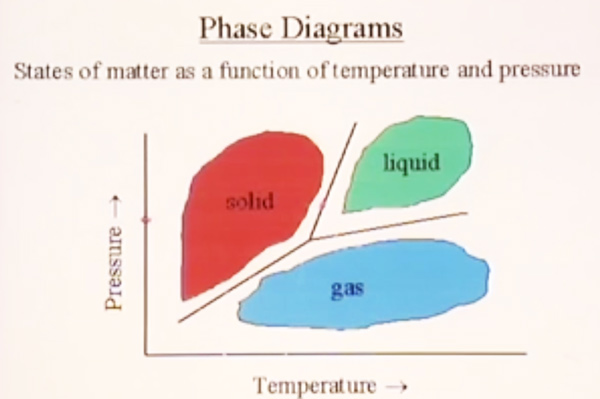
\includegraphics[scale=0.65]{\pIImages/lec33_phase_diagram}
\end{center}

Consider starting at a low pressure, with the temperature at about the center, say around the ``g'' in gas. Clearly, the substance is a gas at this point. We increase the pressure,  while keeping the temperature constant. The volume decreases, and the pressure increases, with $P V$ being kept constant (which is called Boyle's law; it states that $P \propto \frac{1}{V}$ or $PV = \text{constant}$ if temperature/amount of gas is held constant). The ideal gas law holds until we reach the dividing line into the liquid. At this point, \emph{some} of the gas will turn into a liquid, and there will be an equilibrium between the two.\\
If we try to push down harder, the pressure \emph{will not increase} until \emph{all} the gas has been converted into a liquid. Only at that point will pressing harder again increase the pressure; while there is still gas present, pressing down harder will only convert more of the gas into liquid.

Suppose we instead do this at a lower temperature; we can then see that there comes a point in this example phase diagram where we go directly from gas to solid (this is called \emph{deposition}; the reverse process, solid to gas, is called \emph{sublimation}). So we increase the pressure and decrease the volume, until the solid starts forming. Once again, we can't increase the pressure further until all gas molecules are part of the solid.

Let's now look at the case of constant pressure instead of constant temperature.\\
We start out in the solid phase, at about the vertical center -- at the tiny red mark in the $y$ axis, about next to the ``e'' in pressure.\\
Say we start out with water ice; or even iron. We heat it, keeping the pressure constant, meaning we move horizontally towards the right. We eventually hit the dividing line between solid and liquid, i.e. the substance will begin to melt.\\
Once that happens, the temperature will stop increasing until \emph{all} of the solid has melted into liquid, similarly to what we saw with pressure above. Once all of it has become a liquid, we can increase the temperature further.\\
If we do so, it will eventually boil, i.e. go from a liquid to a gaseous form. Yet again, we can no longer increase the temperature at this point, until all of the liquid has become a gas (water vapor). This might be the only one of these that we are familiar with: when boiling water, it doesn't matter if the platter is just barely hot enough than necessary, or \emph{much} hotter than necessary. In either case, the liquid water will not become any hotter than 100 degrees C (unless the pressure is greater than 1 atm), no matter how violent the boiling is.

As a side note: water vapor is completely invisible (it as as transparent as clean air). Any time we think we see water vapor, for example when boiling water in the kitchen, what we actually see is tiny condensed liquid droplets. The water vapor condenses back into liquid as it comes in contact with the much colder surrounding air.\\
For this reason, you may be able to see that just above the surface of boiling water, there is invisible water vapor (i.e. it looks as if there's only air there), and only \emph{above} that is the visible steam showing up, since it hasn't had time to cool down yet when just above the surface of the boiling water.

\subsection{Pressure and phase in a CO2 fire extinguisher}

Carbon dioxide fire extinguishers are fairly common. They work by displacing oxygen, so that a fire can't be sustained. This has two important meanings, by the way: one, it can be dangerous to use on/near people or in closed spaces, as you may suffocate; two, burning materials that contain enough oxygen by themselves may well keep on burning.
 
So is there gas or liquid (or even a solid?) inside such a fire extinguisher?\\
Prof. Lewin calculated the volume of one such extinguisher to be $\SI{7.1e-3}{m^3}$. It is at room temperature, so $T = \SI{293}{K}$.

To find the pressure, which helps us find the phase, we now need to know $n$, the number of moles of CO2 inside. By reading on the label, we can find that the difference between a full extinguisher and an empty one is about 10 pounds, or 4500 grams.

Carbon has an atomic weight of about 12, and oxygen one of about 16; that gives us $A = 12 + 2\times 16 = 44$. With a molar mass of 44 g/mol, we can simply find the number of moles as

\begin{equation}
n = \frac{\SI{4500}{g}}{\SI{44}{g/mol}} = \SI{102.28}{mol} \approx \SI{100}{mol}
\end{equation}

We now have all we need to know to use the ideal gas law. We aren't sure if it will hold, but let's try. Plugging the values in,

\begin{equation}
P = \frac{n R T}{V} = \frac{ (\SI{100}{mol})(\SI{8.31}{J/(K mol)})(\SI{293}{K})}{\SI{7.1e-3}{m^3}} = \SI{3.43e7}{Pa} \approx \SI{340}{atm}
\end{equation}

This pretty much rules out the possibility of there being gas inside, for two reasons! First, it seems doubtful that the container could withstand such a tremendous pressure. Second, if we look at a phase diagram, we would likely find that CO2 becomes a liquid (or a solid) at a way lower pressure than 340 atm at room temperature. And indeed, looking at one, we find that at room temperature, the phase transition to liquid happens at something like 60-70 atm.

The answer is that the extinguisher contains a pressure of about 60 atm, according to a fire department called by the professor. Looking at a phase diagram of CO2, this makes it clear that there is either 100\% liquid, or a combination of liquid and gas inside. When we open the valve, some of the liquid will turn into gas, but the pressure will not change until all the liquid is gone. Up until that point, they must exist together, which can only happen at certain combinations of temperature and pressure. For a \emph{fixed} temperature (say 20 C), however, there is only one pressure at which this can happen; that pressure must then be constant inside until the liquid ``runs out'', having been converted into gas.

This also means we can fit a lot more CO2 into a canister than we could otherwise. Remember how the original calculations said the pressure would have to be over 300 atm if it were pure gas; with this part-liquid mix, we can fit that same amount at about 60 atm instead, which doesn't require as strong a canister. This is put to the test in a lecture question:

``The density of liquid carbon dioxide is about $\SI{0.8}{g/cm^3}$. What volume fraction inside the fire extinguisher (when it is full) is occupied by liquid CO2 ? (The density of CO2 gas is negligible compared to the density of liquid CO2)

Hint: Review what is given in the lecture: Volume of the extinguisher is $\SI{7.1e-3}{m^3}$ , total mass of CO2 = 4.5 kg, temperature= 293 K , pressure at that temperature has to be $\SI{60e5}{Pa}$.''

Hmm. Well, if 100\% was liquid, its volume would be

\begin{equation}
V = \frac{M}{\rho} = \frac{\SI{4500}{g}}{\SI{0.8}{g/cm^3}} = \SI{5625}{cm^3}
\end{equation}

... which is less than the full volume of \SI{7100}{cm^3}. In fact, it is about 80\%... a little more than 75\%, which is one of the answer options. We were told that the density of CO2 gas in negligible, so this should in fact be the answer, and it is. Not a very rigorous process, but they did tell us to neglect the gaseous portion.

\subsection{Isothermal atmosphere}

We have earlier looked at hydrostatic pressure, and found the relationship

\begin{equation}
\frac{dP}{dy} = - \rho g
\end{equation}

between pressure, density and depth. Because we can treat both $g$ and $\rho$ as constants (depth differences are small enough, and liquids are practically incompressible, respectively), this gives us a very simple linear relationship

\begin{equation}
P_2 - P_1 = -\rho g (y_2 - y_1)
\end{equation}

where $y_2 > y_1$ (positive upwards), and therefore $P_1 > P_2$. If you ever lose track of the minus signs and that, you just need to keep in mind that pressure must \emph{increase} at greater depths, and you can't go wrong. With that in mind, I probably prefer to think of this as

\begin{equation}
|\Delta P| = \rho g |\Delta y|
\end{equation}

which is hard to get wrong, using the above (rather obvious) trick.

The reason that was easy to do is that we could treat $\rho$ as constant, with little loss of accuracy. In reality, $\rho$ is a function of pressure. This is a smaller detail for liquids, but a crucial one for gases, which we'll look at now. We can no longer treat $\rho$ as a constant.

We will now look how the pressure changes in altitude in our atmosphere. We will assume that the temperature everywhere is 0 degrees C everywhere in the atmosphere; that is not true, but the full calculation is still a bit too complex. We call this simplification an isothermal atmosphere. (In general, the iso- prefix is used in physics for things that are the same in one way or another; from the Greek word isos, meaning equal.)

Density is mass per unit volume, so if we have $N$ molecules inside a certain volume $V$, each of mass $m$, we can say that

\begin{equation}
\rho = \frac{N m}{V}
\end{equation}

where $\rho$ is the average density inside that volume.

Using the ideal gas law,

\begin{align}
PV &= N k T\\
\frac{P}{k T} &= \frac{N}{V}
\end{align}

So we substitute that, and find

\begin{equation}
\rho = \frac{P m}{k T}
\end{equation}

We can then substitute that into the differential form we had earlier,

\begin{equation}
\frac{dP}{dy} = - \rho g = - \frac{P m }{k T} g
\end{equation}

Rearranged,

\begin{equation}
\frac{dP}{P}  = - \frac{m g}{k T} dy
\end{equation}

As it was before, this is a separable differential equation. $m$ is a constant, $k$ is a constant, and we said we consider $T$ and $g$ constants. The right-hand side is an easy integral, and the left-hand side isn't much harder. We integrate from $0$ (sea level) and $P_0$ to $h$ and $P_h$:

\begin{align}
\int_{P_0}^{P_h} \frac{dP}{P}  &= - \frac{m g}{k T} \int_0^h dy\\
\ln P_h - \ln P_0  &= - \frac{m g}{k T} h\\
\ln \frac{P_h}{P_0} &= - \frac{m g}{k T} h
\end{align}

Exponentiating both sides:

\begin{equation}
\frac{P_h}{P_0} = e^{- \frac{m g}{k T} h}
\end{equation}

We can still simplify this a bit. We have a constant involved; we can find its value. If we flip it upside down, the constant I'm talking about is

\begin{equation}
H_0 = \frac{k T}{m g}
\end{equation}

This is called the \emph{scale height}; it has the dimension of length, because its reciprocal (in the exponential above) must be 1 over length, so that it cancels out with $h$; you need a dimensionless number in exponentials. We know $k = R/N_A \approx \SI{1.38e-23}{J/K}$, $T = \SI{273}{K}$ (0 degrees C, as we chose earlier), and $g \approx \SI{9.8}{m/s^2}$. What about $m$, the mass of an air molecule?

Well, the professor chose to use 29 atomic mass units, with this reasoning: air is about 20\% oxygen (32 amu per molecule) and about 80\% nitrogen (28 amu per molecule), and some spare change (argon, CO2 etc) that we ignore. Since there is more nitrogen, we choose a number closer to 28 than 32 amu, and so we end up with 29 amu. (The actual value appears to be 28.964, so this approximation is very good.)\\
Each amu represents a mass of about $\SI{1.66e-27}{kg}$, so all in all, we find $H_0 \approx 8000$ meters. Rewriting our exponential, we now have

\begin{equation}
P_h = P_0 e^{- h/H_0}
\end{equation}

Using $H_0 = 8$ km and $P_0 = 1$ atm, we can then for example find that the air pressure at 3 km above sea level is about $(\SI{1}{atm})e^{-3/8}$, or about 0.7 atmospheres. At 8 km, it is only $1/e$ times 1 atm, which is about 0.37 atmospheres.

This not only has implications for human life (the air is basically too thin to support human life, though some do climb Mount Everest with no supplemental oxygen), but also for basic things like boiling water.\\
The boiling point is defined as the temperature where the liquid's \emph{vapor pressure} (which we have not really learned about in this course) equals the (atmospheric) pressure of the air surrounding the liquid.\\
The vapor pressure of a substance, e.g. water, is a constant for a given temperature. At 100 degrees, it is about 101.3 kPa (1 atm) -- that is to say, it boils at 100 degrees at 1 atmosphere. However, if the atmospheric pressure is \emph{lower}, the water will boil at a lower temperature. For example, water would boil at 80 degrees C if the atmospheric pressure were 47.3 kPa (about half an atmosphere); in other words, the vapor pressure of water is 47.3 kPa at 80 degrees C.\\
This can cause some trouble for cooking at higher altitudes -- in extreme cases, it will be hard to prepare certain types of food as they will need to boil for very long.

Even more interestingly, the vapor pressure of water at 22 degrees C is about 2.6 kPa -- which means that if we place water in a near-vacuum, it will boil at or even below room temperature. This is demonstrated in the lecture.\\
To see this on a phase diagram, locate the (likely vertical) line of constant temperature of about 20 degrees, and then find the point along that line of 1 atmosphere pressure. That's where we start out; you will undoubtedly find that the water should be in its liquid phase. Follow that line of constant temperature downwards, and you will eventually reach the line where gas and liquid coexist -- which is where it starts to boil.

\subsection{More lecture experiments}

A second lecture experiment is to add a very small amount of liquid water to a paint can (of the same type that imploded in a previous lecture, when we sucked out the air from inside it), boil it, and then seal the can. It is now filled with almost 100\% water vapor (a tiny fraction liquid water may remain), at 100 degrees C, and 1 atmosphere of pressure. We seal the can, and let it cool.

The amount of water, in moles, must of course be a constant. However, now that the temperature goes down, so does the volume of the water vapor gas; we can see this by looking at the vapor pressure for water at various temperatures. (Perhaps also by using the ideal gas law, but it doesn't hold very well for water vapor.)\\
Indeed, as it cools back down to room temperature, the vapor pressure is about 1/45 atm, so there is practically a vacuum inside (as far as the thin walls are concerned, at least), and the can will implode.

Next, we cool a regular air-filled balloon in liquid nitrogen. We change the temperature of the air inside from 293 K to about 77 K (about -196 C, the boiling point of liquid nitrogen). What will happen to the balloon?\\
We can see, using the ideal gas law, that it must shrink; if we hold $P$ approximately constant, that is clear.

\begin{align}
V_1 &= \frac{n R T_1}{P}\\
V_2 &= \frac{n R T_2}{P}\\
\frac{V_2}{V_1} &= \frac{T_2} {T_1}
\end{align}

This gives us $V_2/V_1 \approx 0.26$. The radius changes less, though; $R \propto V^{1/3}$, so the radius should shrink by something like 60\%. However, in practice, the balloon shrinks down to almost nothing -- the volume goes down to perhaps 1-2\% of the original, or something of that order.

What did we miss? Well, we used the ideal gas law -- but we won't have gases when we're done! Remember that air is 80\% nitrogen, and we dip it into liquid nitrogen. The nitrogen inside the balloon may turn into liquid, since we cool it to approximately\footnote{The heat transfer may not be ideal, etc., so it may not go all the way down to 77 K.} its boiling point.\\
The boiling point of oxygen at 1 atm is about 90.1 K, so we cool that down below its boiling point, too, so the oxygen should certainly become a liquid. We know, of course, that liquids have a \emph{way} higher density than gases, so it should not come as a huge surprise (when you consider the phase changes) that the volume is very small.

\section{Lecture 34:Heisenberg's uncertainty principle}

\subsection{Off-topic intro}

This is a course on classical mechanics. It is extremely useful in many everyday situations, whether we talk about toy gyroscopes, elastic collisions in billiards or in all kinds of mechanical engineering. However, it it doesn't always hold true. At large velocities or in very strong gravitational fields, the laws of physics we've learned about here gradually become more and more incorrect. The velocities involved are on the order of 1/10 of the speed of light and greater (or a bit less, depending on the accuracy required); here, we need Einstein's theory of special relativity to find correct answers. For example, using what we have learned in this course, we can calculate the kinetic energy of a 1 kg mass moving at the speed of light as $\frac{1}{2} (\SI{1}{kg}) c^2 \approx \SI{4.5e16}{J}$, but this is a meaningless result. It would take an infinite amount of energy to accelerate a mass to that speed, and so via the work-energy theorem it would have an infinite kinetic energy.

The actual kinetic energy is found as

\begin{equation}
K_e = m \gamma c^2 - m c^2 = m c^2 \left( \frac{1}{\sqrt{1 - v^2/c^2}} - 1 \right)
\end{equation}

Note that as $v \to c$, $K_e \to \infty$, which is not the case in Newtonian mechanics. If you try to plug in $v > c$, you get an imaginary result with no physical meaning.

If we calculate the Taylor expansion of the above function centered at $v = 0$ and only keep the lowest-order term, $\frac{1}{2} m v^2$ is the only term that remains. That is, classical physics agrees with special relativity, only that the latter can handle the more extreme cases.\\
If we plot these two functions between $v = 0$ and $v = 10^7$ m/s, they are almost impossible to tell apart. The plot starts to visually diverge at about $\SI{3e7}{m/s}$, where Einstein's version gives $\SI{4.534e14}{J}$ and the classical variant only $\SI{4.500e14}{J}$.

The term

\begin{equation}
\gamma = \frac{1}{\sqrt{1 - v^2/c^2}}
\end{equation}

is called the Lorentz factor, and appears in many special relativity equations, regarding kinetic energy, momentum, time dilation, length contraction and probably other things I'm not yet aware of. It is a useful thing to know even if you only know Newtonian mechanics: the closer $\gamma$ is to 1, the more accurate the physics we've learned so far will be. For everyday speeds below 200 km/h, $\gamma$ is still 1 to within well over 10 decimal points. At 1000 km/s (yes, per second!), it is about 1.00000556, so calculating momentum as $m v$ instead of $m v \gamma$ will yield an error of much less than 1\%. At $10^8$ m/s, 1/3 the speed of light, $\gamma$ is \emph{still} only 1.06, though this is about where it starts to shoot off towards infinity and begins to truly matter.

Now for a much quicker look on gravity.\\
As an example, the orbit of Mercury cannot be predicted accurately using Newton's law of universal gravitation; its orbit precesses, at a rate of about 1.55 degrees per century relative to the Earth. Einstein's theory of general relativity explains this anomaly, and is currently the best theory of gravity we have. As mentioned, though, classical mechanics is still ``correct enough'' for the vast majority of applications. General relativity is heavily used in astrophysics, where it describes many things that Newtonian mechanics does not (and describes the rest of them more accurately), one of which is gravitational lensing: light bending in gravitational fields.

I had to add a subsection label to this as it became a bit too strongly off topic -- I was going to write a few short sentences on the limits of classical mechanics and simply introduce relativity and quantum mechanics, but got a bit carried away!

\subsection{The smaller world}

After that off-topic introduction, let's now look at the second case where Newtonian mechanics stops working: the world of the very small, i.e. the atomic and sub-atomic scale.\\
An atom is about $10^{-10}$ meters, including the surrounding electron cloud. The nucleus itself is much, much smaller yet, and yet it contains virtually 100\% of the atom's mass. The distance between the nucleus and the electrons is on the order of 100 000 times greater than the size of the nucleus.\\
The nucleus consists of protons (positively charged) and neutrons (with no electric change, thus the name) bound together by the strong nuclear force, which is much stronger than the electromagnetic force, but has an extremely short range, on the order of a nucleus and less. The strong nuclear force is the reason why the nucleus can be held together despite the electromagnetic repulsion of the equal charges; without it, all nuclei would simply fall apart. (Neutrons and protons themselves couldn't exist without it either, as the quarks that make \emph{them} up are also held together by the strong force.)

Atoms are basically all vacuum, as we can see above (the nucleus is almost zero size compared to the atom's total size) -- we're used to thinking of ``empty'' spaces being filled with air, but since air \emph{consists} of atoms, well, there isn't much of anything that fits inside an atom!\footnote{In quantum physics, there \emph{are} ``things'' inside this vacuum: empty space is not truly empty, but contains random energy fluctuations and short-lived virtual particles, in what's called a quantum foam. I won't (and can't!) go into more detail, though.}
So why can we not walk through walls, if we all consist of mostly vacuum? The professor mentions that it's not easy to answer and that we cannot answer it using classical physics, which I find surprising.\\
All (neutral) atoms have electrons in ``shells'' surrounding the nucleus. All electrons are negatively charged, and like charges repel; therefore, atoms repel each other. Your hands are being repelled by the wall even when you're standing ten meters from the wall, but with a force small enough that you cannot notice it. When you are ``touching'' the wall, the repulsive force is very large, and the closer you try to come, the stronger the repulsive force. That is, you never really touch a wall -- just you get really, really close, and the normal force the wall exerts on you really comes from this electromagnetic repulsion of the electron shells.

As far as I know, the above explanation is fairly correct, and if not else a useful way to think of it. I'm not sure of the details of it, however. There must be a reason the professor didn't use it, and especially mentioned that it cannot be explained by classical physics.

In 1913, Danish physicist Niels Bohr postulated that electrons move around the nucleus in well-defined energy levels, which are all distinctly separated from each other, and that electrons cannot exist in between these allowed energy levels. This is then the reason why the electron does not simply crash into the nucleus, as it would seem like it should, considering the electromagnetic attraction between the two.

This concept of quantization was groundbreaking. It also implies that planetary orbits should be quantized; you couldn't orbit at an arbitrary distance, so that you couldn't move an object in orbit in or out just a tiny bit.\\
it also implies that we can't bounce a tennis ball on the ground and have it reach any level; instead, there would be a set of allowed heights it could reach.

However, the quantization here is on a very, very small scale. Small enough that we could never measure the effect on the scale of planetary orbits or tennis balls; the effect is \emph{much} too tiny for that. It is for exactly this reason that quantum mechanics has no meaning when it comes to the motion of tennis balls and planets.\\
Some quantum phenomena are absolutely observable in daily life, however: magnetism has its origin in quantum physics, for example. We will also soon perform an experiment where we could say that quantum physics is observable using the naked eye.

The professor stresses this point of quantized electron energy levels, as it is a very important one.

When we heat a substance, the electrons can gain energy, and therefore jump to higher energy levels. Later on, they lose that energy, and fall back down. As they do, they emit photons: they need to lose that extra energy somehow (since the higher energy levels have, well, higher energy than their previous states).\\
The professor makes an analogy with the work you do while lifting a vase in a gravitational field. You do work, but that energy is not lost; if you drop the vase, the stored gravitational potential energy is ``released'' by being converted into kinetic energy.

\subsection{Photon energy and momentum}

The energy of a photon can be written as

\begin{equation}
E = h f = \frac{h c}{\lambda}
\end{equation}

where $h$ is the Planck constant, $h \approx \SI{6.6e-34}{J s}$, perhaps the most important constant in all of quantum physics. There is also the related constant $\hbar$, ``h-bar'', which is $\hbar = \dfrac{h}{2\pi} \approx \SI{1.05e-34}{J s}$.\\
$f$ is the photon's frequency in hertz, and $\lambda$ the wavelength in meters.

This definition makes it clear that the greater the photon's energy, the shorter the wavelength, and vice versa.\\
This also means that when an electron jumps from a high to a low energy state, and the energy difference between the two levels is very high, a short-wavelength photon will be generated, since it must contain all the energy of the jump. (A single energy jump always releases exactly one photon; an electron can fall down multiple levels in \emph{steps} however, in which case one photon is released per step. These photons will then have a smaller individual energy than if the entire jump were to be done in one step.)

Here's a diagram illustrating these energy jumps.

\begin{center}
\includegraphics[scale=0.65]{\pIImages/lec34_energy_levels}
\end{center}

The lowest-drawn line is the lowest allowed energy level, with energy increasing towards the higher levels.\\
A jump from the highest energy level to the lowest one may generate a photon with too much energy (too short a wavelength) to be visible -- ultraviolet (or even beyond that), while some of the smaller jumps may correspond to visible wavelengths: blue for the more energetic visible ones, green for the mid-range ones, red for the lowest-energy visible jumps. Finally, even smaller jumps may generate invisible frequencies again, such as infrared or beyond.

So when a material emits photons in this manner, we expect to see these very discrete photon wavelengths, and nothing at all in between. Indeed, we can test this. By using a diffraction grating (a concept later introduced in 8.02/8.02x), we can split the light into its constituent colors, in concept not unlike a prism, so that we see the colors laid out in a nice horizontal line, looking very much like pictures of emission and absorption spectra that we have seen earlier, e.g. like this:

%TODO: add image
%\begin{center}
%\includegraphics[scale=0.65]{\pIImages/lec23_hydrogen_emission}
%\end{center}

This is what we would expect to see from a pure-hydrogen source emitting light.

\begin{center}
$\vcenter{\hbox{\includegraphics[scale=0.65]{\pIImages/lec34_helium_grating}}}$
$\vcenter{\hbox{\includegraphics[scale=0.65]{\pIImages/lec34_neon_grating}}}$
\end{center}

Above are two ``simulations'' of the gratings given to the students in lecture, as they could not capture the effect on video. The image on the left is from a helium light source, while that on the right is from a neon light source.

Surprisingly, light also carries momentum! We know that in classical mechanics, $p = m v$, which clearly cannot hold for a photon (if they indeed have nonzero momentum), without some fancy tweaking; the mass of a photon is exactly zero, so $m v = 0$.\\
What we do instead is to use Einstein's mass-energy equivalence, the famous $E = m c^2$:

\begin{equation}
m = \frac{E}{c^2} \Rightarrow p = \frac{E}{c^2} v \Rightarrow p = \frac{E}{c}
\end{equation}

... since $v = c$ for a photon.

We can also find this more directly from the full, less-famous version of the equation:

\begin{equation}
E^2 = (m_0 c^2)^2 + (p c)^2
\end{equation}
where $m_0$ is the rest mass (which I denoted by $m$ above). Since $m_0 = 0$, the equation simplifies down considerably to

\begin{equation}
E = p c
\end{equation}

which is what we found before.

This momentum also gives rise to interesting properties such as radiation pressure/light pressure: shining a light onto something causes a pressure (and therefore a force) due to this momentum transfer! This is used in practice to create spacecraft with ``solar sails'' that use the momentum transfer from reflected light to accelerate. The effect is too tiny to be noticed in daily life, though, considering that visible light has a momentum on the order of perhaps $10^{-27}$ kg m/s per photon. Despite that they come in large numbers, the radiation pressure of for example a regular lamp is negligibly small compared to just about any other force we experience.

\subsection{Wavelength of a particle}

Before quantum mechanics, physicists were divided into two camps: those who thought light to consist of particles, and those who thought it was made of waves.\\
Newton believed that light was made of particles, while Dutch physicist Huygens believed they were waves.\\
In 1801, British scientist Thomas Young showed fairly conclusively that light is a wave, by performing the famous double-slit experiment.\\
You shine a monochromatic light onto two very thin slits in some material (that otherwise blocks light), and project that onto some surface a distance behind.\\
What you see is an interference pattern: there is bright light at the center, then darkness a bit further out, then light again even further out, etc. This can be ``easily'' explained (and is discussed in detail in 8.02/8.02x, and likely even more in detail in 8.03) in terms of light being a wave, as the peaks of the wave cancel out with the valleys when the two arrive in phase, causing darkness; likewise, when two peaks arrive in phase, they add instead of cancel, and the result is a bright area.\\
The two forms of interference are called destructive and constructive interference, respectively.

So it looked like Huygens was right; light is a wave. However, later on, experiments were made that showed quite conclusively that light is made up of particles, perhaps most notably the photoelectric effect observed by Einstein (which won him his only Nobel prize) that required light to arrive in quantized ``packets'' of energy, rather than in a continuous wave. (Einstein didn't discover the effect itself, however.)

Quantum mechanics says the answer to this disagreement is that light acts as \emph{both}, depending on the situation; this concept is known as wave-particle duality.

One of the truly strange things about quantum mechanics is that we can consider \emph{matter particles} to be waves, as well. We now know that finding the wavelength of a photon of some given energy is easy, but what about the wavelength of an electron, or of a baseball?\\
Louis de Broglie suggested that matter can act as waves in this manner. He also specified that the wavelength of such a particle would be

\begin{equation}
\lambda = \frac{h}{p}
\end{equation}

where $p$ is simply the momentum $m v$. We can derive this result ourselves using what we know of the momentum of light.

We know that $E = p c$ and $\displaystyle E = h f = \frac{h c}{\lambda}$; if we put these together, we find

\begin{equation}
p c = \frac{h c}{\lambda} \Rightarrow  p = \frac{h}{\lambda}
\end{equation}

or, equivalently, $\displaystyle \lambda = \frac{h}{p} = \frac{h}{m v}$. This wavelength is called the \emph{de Broglie wavelength}, after him. This derivation assumes that the result is equally valid for matter particles as it is for light, though, which is by no means obvious.

Note that if the momentum is higher, the wavelength is shorter. An electron moving at $10^7$ m/s, and with a rest mass on the order of $10^{-30}$ kg ($9.1\times 10^{-31}$ kg) has a classical momentum of about $\SI{9.1e-24}{kg m/s}$, which translates into a wavelength of about $\lambda = \SI{7.25e-11}{m}$ -- about 73 picometers, several times larger than at atomic nucleus.

A daily life-sized object such a baseball, with a mass of 145 grams, moving at 130 km/h (36.11 m/s) has a momentum of about $5.24$ kg m/s, which gives it a de Broglie wavelength of about $1.3 \times 10^{-34}$ meters -- which is of course ridiculously small. It's far, far below what we could ever measure directly (at a billion billion times smaller than a proton), so this wavelength is meaningless in the macroscopic world. These kinds of quantum effects simply aren't observable at this scale.

\subsection{Heisenberg's uncertainty principle}

In 1926, Austrian physicist Erwin Schr\"odinger formulated the Sch\"odinger equation, which is at the heart of quantum mechanics; it is a wave equation, which describes how a quantum system evolves over time. It unifies these wave and particle behaviors into one set of rules.

We talked earlier about the double-slit experiment and interference of waves. Amazingly, we can do this experiment with particles, too, and get the same end result! This is one of the many extremely nonintuitive results we can find in quantum mechanics.\\
It seems bizarre that e.g. two electrons can be shot through two slits, and then combine and disappear. We really need to think in terms of waves for this to make any sense at all; if the electrons are instead two waves moving through the slits, it does make sense that they can cancel each other out at certain locations.

Let's now look at another bizarre effect in the quantum world. In classical physics, we can measure the momentum and position of an object with any precision that we need, as long as we have the equipment and cleverness. The object has a certain mass, and we can measure its position and momentum at the same time with no problems.

In quantum mechanics, this is not possible. We can measure the position to an arbitrary accuracy, and the momentum to an arbitrary accuracy, but not at the same time! The more exactly we know one, the less exactly we know the other, in this one measurement. This is known as Heisenberg's uncertainty principle.

``The very concept of exact position of an object and its exact momentum, together, have no meaning in nature.''

One way of writing this down mathematically is

\begin{equation}
\Delta p \Delta x \overset{>}{\approx} \frac{\hbar}{2}
\end{equation}

where again $\displaystyle \hbar = \frac{h}{2\pi} \approx 10^{-34}$ joule-seconds.\\
The right-hand side is often written as a factor 2 larger, and I'm not sure which we actually should use. The principle is also often stated in terms of standard deviations. I think we'll have to accept that this is approximate, and take a proper quantum mechanics course for more detail.

Roughly speaking, then, if we know the position to an accuracy $\Delta x$, the momentum is non-determined by an amount

\begin{equation}
\Delta p \overset{>}{\approx} \frac{\hbar}{2 \Delta x}
\end{equation}

The lecture uses twice this ($\hbar$ rather than $\hbar/2$), but there was a caption suggesting that the above values are the ones that \emph{should} have been used in the lecture, i.e. a post-recording correction, so I chose to use their corrected information instead of the one actually shown in the lecture video itself.

The professor uses a story from a book, trying to describe quantum mechanics in an intuitive way (more or less). In this story, we set $\hbar = 1$, instead of about $10^{-34}$. This essentially has the effect of scaling up these quantum effects to a level where we can observe them.\\
So in this world where $\hbar = 1$, a character in the book takes a billiard ball and puts it in a triangle (which is used to align the balls at the start of the game; it can fit exactly 15 such balls in the case of pool).

Assuming the ball stays inside the triangle (which may not be a safe assumption in this crazy quantum world; see quantum tunneling), we have constrained its position to $\Delta x \approx 0.3$ meters. We \emph{know} that it must be somewhere inside the triangle. Via Heisenberg's uncertainty principle, this implies that the ball's momentum is ill-defined to about $1/0.3$ kg m/s (using $\hbar = 1$, and using $\Delta x \Delta p \overset{>}{\approx} \hbar$, as in the lecture), so about 3 kg m/s. If the ball has a mass of 1 kg, the ball's velocity is undetermined to about 3 m/s -- $\Delta p = m \Delta v$. It's moving around like crazy, simply because we constrained its position.

Professor Lewin reads a passage from the book (``the professor'' in what follows refers to a character in the book):

``Look here'', the professor said. ``I'm going to put definite limits on the position of this ball by putting it inside a wooden triangle.''\\
As soon as the ball was placed in the enclosure, the whole inside of the triangle became filled up with the glittering of ivory.\\
''You see'', said the professor, ''I defined the position of the ball to the extent of the dimensions of the triangle. This results in considerable uncertainty in the velocity, and the ball is moving rapidly inside the boundary.\\
''Can't you stop it?'', asks Mr. Tompkins.\\
''No, it is physically impossible. Any body in an enclosed space possess a certain motion. We physicists call it zero point motion. For example, the motion of electrons in any atom.''

So with $\hbar = 1$, the bizarre consequences of the quantum world become more apparent to us, though hardly much easier to grasp.\\
What happens when we perform this experiment in the real world? Well, we perform the same math, but with $\hbar$ being $10^{-34}$ times smaller than above. The effects scales linearly with $\hbar$, so the uncertainty in the ball's velocity is now on the order of $\SI{3e-34}{m/s}$ -- a value so tiny that we could never measure it. In one billion years, the ball would move at most 1/100 of the diameter of a proton. Such distances and velocities are of course completely meaningless to us, and so we again see that these effects are irrelevant in the macroscopic world ``of baseballs and billiards and pots and pans''.

For this reason, it is no problem for us to talk about a billiard ball being exactly at a certain position, and having exactly zero speed. The error is so far beyond measurable that we could never show whether it actually exists or not, so it is completely safe to ignore it and keep working as usual.

Let's now look at an atom, and more specifically the electrons ``orbiting'' it. Say an atom is about $10^{-10}$ meters. An electron is then confined to $\Delta x \approx 10^{-10}$ m. Using the uncertainty principle, we can find that

\begin{align}
m \Delta v \Delta x &\overset{>}{\approx} \hbar\\
\Delta v  &\overset{>}{\approx} \frac{\hbar}{m \Delta x}
\end{align}

(Again, this is using the lecture's possibly incorrect equations and not the ones they later added as corrections via overlaid text, though I'm not sure if either form can be used for accurate calculations.)\\
Using $\Delta x = 10^{-10}$ m and $m \approx 10^{-30}$, we find $\Delta v \overset{>}{\approx} 10^6$ m/s, a third of a percent of the speed of light. So the electron moves simply because it is confined.

\subsection{The single-slit experiment}

The professor then makes a demonstration that can be explained in terms of the uncertainty principle. We shine a laser beam, monochromatic light (i.e. it consists of only one wavelength, as opposed to e.g. white light) onto a thin vertical slit in a material that otherwise blocks light. A distance $L$ away (where $L$ is several meters), we have a wall, that this light pattern is projected upon.

During the experiment, we then shrink the (vertical) slit's width. In doing so, less light will manage to pass through -- that much is clearly unavoidable -- and the laser dot projected on the wall will have its sides ``chopped off'', just as we would predict.\\
However, in doing this, we are constraining $\Delta x$. The thinner the slit is, the better we know the $x$ position of the photons that pass through (if we consider them as photons rather than waves, that is). Because of this, via the uncertainty principle, we lose accuracy in our knowledge of the momentum in the $x$ direction (the direction we are constraining the photons in).
We are not constraining the beam in the $y$ directions, so nothing out of the ordinary will happen in the vertical direction.\\
Horizontally, however, the light begins to \emph{spread out}. The \emph{thinner} the slit becomes, the \emph{wider} the light projection becomes! Simply because we reduce $\Delta x$ and constrain the light's position, the x-component of the momentum is starting to become more and more ill-defined, and some of the light spreads out accordingly.

We can work this out semi-quantitatively. The momentum of each photon is about $10^{-27}$ kg m/s, according to the professor. This indeed corresponds to the wavelength of red light; the laser in the lecture is green, but everything here is an order-of-magnitude approximation, so there's little point in being more precise.\\
Say we start with the slit at 1/10 mm, that is, it can pass though a slit of width $\Delta x \approx 10^{-4}$ meters, constraining its position. That makes the x-component of the momentum ill-defined to about $h/\Delta x \approx 10^{-34} / 10^{-4} = 10^{-30}$ meters. (I'm not sure if $\hbar$ was/should be used here, but it seems it was not; consider this an order-of-magnitude type result either way.)

The total momentum is then the sum of the light's original momentum and this $\Delta p$, so the path changes path according to this vector addition:

\begin{center}
\includegraphics[scale=0.65]{\pIImages/lec34_momentum_uncertainty}
\end{center}

We then expect some of the light to shoot off at an angle, but only in the $x$ direction; the light is not constrained at all in the $y$ direction (the slit's height is much greater than the light beam's diameter).

The angle $\theta$ between the original vector and the new one can now be easily calculated. Using trigonometry, $\tan \theta = \Delta p / p$. For small angles, $\tan \theta \approx \sin \theta \approx \theta$, we can consider this simply as $\theta = \Delta p / p$. (The professor did this implicitly.)

For the values we have, with $\Delta x = 1/10$ mm leading to $\Delta p \approx 10^{-30}$ kg m/s, we find $\theta \approx 10^{-3}$ radians. Using the definition of a radian, we can multiply this by the distance $L$ to the screen to get the approximate size at the screen. With $L = 10$ meters, we find $\theta L \approx 1$ cm (in each direction from the center, so a total width of about 2 cm).

However, if we make the slit 10 times smaller, $\Delta p$ grows by 10 times, which causes $\theta$ to grow by 10 times, and therefore $\theta L$ also grows by 10 times. The ``uncertainty'' is now 10 cm in each direction of the center, so the light has spread out way more. This is then demonstrated in the lecture -- which is clearly something that must be \emph{seen}!

The professor then makes it clear that this can be explained without the uncertainty principle -- and was explained to high accuracy even in the 19th century; this demonstration is however entirely consistent with the uncertainty principle.\\
(This experiment is also discussed in further detail in 8.02/8.02x, in the context of interference of light waves and diffraction; there, we also explain the dark bands that appear, that I briefly mentioned in regards to the \emph{double} slit experiment, where they are more prominent and appear in two ways, rather than one way as seen here.)

Modern quantum physics can make some incredibly accurate predictions (I read that in some cases, we can measure quantum phenomena to an accuracy a million times better than that of some astronomical phenomena), however, we cannot predict exactly where each photon is going to end up. Quantum mechanics is, by its very nature, a probability-based theory. We can calculate how the pattern will look after a whole lot of photons have hit the screen, as they are more likely to end up in some places. However, we cannot predict anything at all about what an individual photon will do; as far as we can tell, nature has an intrinsic randomness built into it.

It has been argued that perhaps this behavior is not random; perhaps it would be predictable, only that there are some variables we are not aware of, and that a more complete theory \emph{would} be able to predict all behavior (given all necessary initial conditions). Certain types of these theories seem to have been disproven, and as of yet, there is no proof of these so-called ``hidden variables'' existing, though there is still discussion and research being done in this area, to the best of my understanding. That is, quantum mechanics still appears to be indeterministic: given all possible information about every particle in the universe, you still cannot predict exactly what will happen next, only come up with accurate probabilities.

One more crazy detail in regards to this: it's important to realize that this experiment cannot be adequately explained by photons (particles) interfering with each other. The exact same pattern will build up over time \emph{regardless} of the rate you shoot the photons through. Even if you shoot one photon, wait 5 minutes, shoot the next, etc. the same pattern will emerge over time. The photon must in some way interfere with... itself? This only really makes any kind of sense if we consider waves.

Also, the same experiment can be and has been done with particles, ranging from electrons up to multi-atom structures such as ``buckyballs'' (each of which consists of 60 carbon atoms), and the results are exactly as predicted by quantum mechanics. Photons, electrons or buckyballs -- nature doesn't really care and treats them the same way, it would seem!

\subsection{Some notes on the uncertainty principle}

(This last section is not at all from the lecture, and is (just as the intro section to this lecture) all written by me. That is, you shouldn't take anything in here as hard fact, as I have not studied quantum mechanics to any greater extent than what this course teaches, plus some popular science which often is just as misleading as it is informative.)

A common question (and misconception) is that this uncertainty is a technical limit in our measuring equipment; it is not. It is a physical limit built into nature. I hardly have the expertise (or even basic knowledge) of quantum mechanics to know this myself yet, but many describe the entire notion of perfectly knowing both momentum and position as \emph{meaningless} in quantum mechanics, including that quote in the lecture earlier.

Another common explanation for this uncertainty (one that I've liked myself) is that in order to for example measure the position of an electron, we need to probe it somehow, perhaps using light (sending photons to interact with it). A photon of long wavelength has little energy and thus little momentum, and won't disturb the electron a lot; we get a fairly accurate measurement of its momentum, but since the light wavelength is large, we don't know \emph{exactly} where it is; we only have a fuzzy idea about the position!

If we want to measure the position accurately, we instead need to use light of a shorter wavelength (smaller $\Delta x$), i.e. greater energy (and greater momentum, $p = E/c$ for light). This means we will know where the electron is (was) very accurately, but because we transferred a large amount of momentum to it, we can now not know its momentum exactly.

The above explanation (Heisenberg's microscope) is not technically accurate, though. It is a metaphor, rather than an explanation. In reality, the uncertainty predicted by the uncertainty principle is greater than that in the above experiment.

My current understanding (again, without having actually studied any quantum mechanics -- this is still unlikely to be 100\% correct!) is that the uncertainty arises from the wave nature of matter. That is, the electron doesn't really \emph{have} a perfectly defined position until it is probed; prior to the probing, the electron's position is only a probability distribution. It may be likely to be confined in a small volume, but it is still \emph{possible} for it to be outside it -- even infinitely far away, only with a probability moving closer to 0 the further away you go.

\section{Lecture 35: Professor Lewin's early days at MIT}

I did not take any notes for this lecture. It is as always absolutely worth watching, but it feels pointless to write it down -- professor Lewin is telling \emph{his} story, and I should leave that to \emph{him} to do so! If you want it in text form, his book ``For the Love of Physics'' talks about  these topics and several others!

%%% Local Variables:
%%% TeX-master: "../../../main"
%%% End:

 \newpage
\newcommand{\pathPII}{\pathPHY/Physics-II} \chapter{Physics II}
This compendium is based on the course notes of MIT 8.02 2004 \url{https://web.mit.edu/8.02t/www/802TEAL3D/visualizations/coursenotes/index.htm} and the lectures of MIT 8.02 by Professor Walter Lewin in 2002. The video lectures can be viewed on YouTube from Lectures by ``Walter Lewin. They will make you \ensuremath\varheartsuit~Physics.'' with the playlist name ``8.02x - MIT Physics II: Electricity and Magnetism''
All credits go to Dr. Sen-ben Liao, Dr. Peter Dourmashkin, and Professor John W. Belcher at MIT for the lecture notes and Professor Walter Lewin for the inspiring lectures. I can not guarantee the accuracy of this compendium and that it is a correct interpretation of the material and explanation provided by the lecture notes and lectures. Thus, for accurate information refer to the material that this compendium is based on. If a mistake is in the compendium it is most likely my fault and not the fault of the material in which this compendium is based on.


\section{Introduction}
\subsection{Electric Charges}
%\section{Electric Charges and Forces and Coulomb's Law - Polarization}
An atom comprises positively charged protons, neutrally charged neutrons, and negatively charged electron.
An atom or molecule can have a neutral, positive or negative electric charge. A negatively charged atom or molecule is called a \textit{negative ion}, meaning to a surplus of electrons compared to protons.
A positively charged atom or molecule is called a \textit{positive ion}.
The nucleus, the protons and neutrons or the atom, is significantly larger than an electron, a proton with a size of $10^{-15}\SI{}{\meter}$ is roughly 1000 times larger than an electron with a size of $10^{-18}\SI{}{\meter}$.
For a hydrogen atom the lower energy state has the most probable distance, using Bohr Radius, of approximately $10^{-11}\SI{}{\meter}$ from the nucleus, which is 10000 times further than the size of the hydrogens' proton.

An intuitive way of thinking why same changed ions repel each other and why opposite charged ions attracted each other is to think about a room where we have loud and talkative people who want someone to listen to them, i.e., negative ions, and quiet, shy listeners, positive ions. When a loud and talkative person is approached by another loud and talkative person they talk over each other and neither gets want they want and find it physically uncomfortable to be near each other, they naturally repel each other. Likewise, if two quite people talk to each other they find it awkward and physically uncomfortable to be close each other. However, if there are a quite, shy listener and a loud talkative person they have found there mach.

Conductors allows electrons to flow ``freely'', there is always some resistance. Continuing with our metaphor we can think of it as a channel where the voice of the loud and talkative person can travel far and reach the quite, shy listener. And non-conductors are like a wall where the voice does not travel through.

\subsection{Polarization}

If we have a positive charge object like we see with the rod in Figure~\ref{fig:charged-rod} placed next to a conductive object like we see with the cloud shaped object next to the rod, the conductive object will have a negative and a positive charged side. Only $10^{13}$ of electrons that was originally on the left side might have moves to the right side.

\begin{figure}[H]
\centering
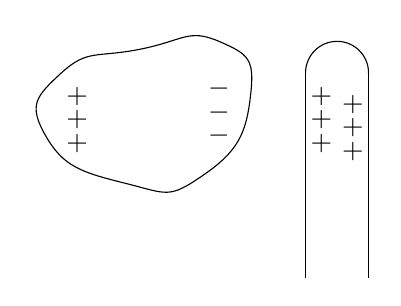
\begin{tikzpicture}

  % Shape of the object
  \path[draw=black]
    plot[smooth cycle, tension=1] coordinates {
      (0,0.4) (1,0.5) (1.4,-0.2)
      (0.8,-1.2) (-0.2,-1.3)
      (-1.2,-0.7) (-1,0.1)
    };

	\node at (-0.8,-0.2) {$+$};
	\node at (-0.8,-0.5) {$+$};
	\node at (-0.8,-0.8) {$+$};

	\node at (1.0,-0.1) {$-$};
	\node at (1.0,-0.4) {$-$};
	\node at (1.0,-0.7) {$-$};


	\draw (2.1,0.1) -- (2.1,-2.5);
	\draw (2.9,0.1) -- (2.9,-2.5);
	\draw (2.1,0.1) arc[start angle=180, end angle=0, radius=4mm];

	\node at (2.3,-0.2) {$+$};
	\node at (2.3,-0.5) {$+$};
	\node at (2.3,-0.8) {$+$};

	\node at (2.7,-0.3) {$+$};
	\node at (2.7,-0.6) {$+$};
	\node at (2.7,-0.9) {$+$};

\end{tikzpicture}
  \caption{Positively charged rod next to some conductive object}
  \label{fig:charged-rod}
\end{figure}

What happens in Figure~\ref{fig:charged-rod} mostly due to induction where the atoms become polarized, i.e., the electron spends more time on one side than the other.
\begin{figure}[H]
\centering
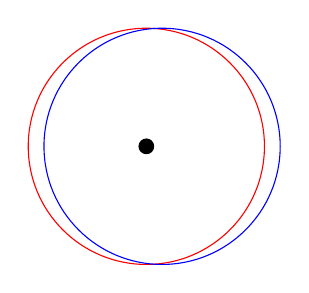
\begin{tikzpicture}

  \fill (0,0) circle (1mm);
  \draw[red] (0,0) circle (15mm);
  \draw[blue] (0.2,0) circle (15mm);

	\end{tikzpicture}
  \caption{Polarized atom is shown with the blue circle and red is non polarized.}
  \label{fig:polarized-atom}
\end{figure}

\begin{figure}[H]
     \centering
     \begin{subfigure}[b]{0.4\textwidth}
         \centering
         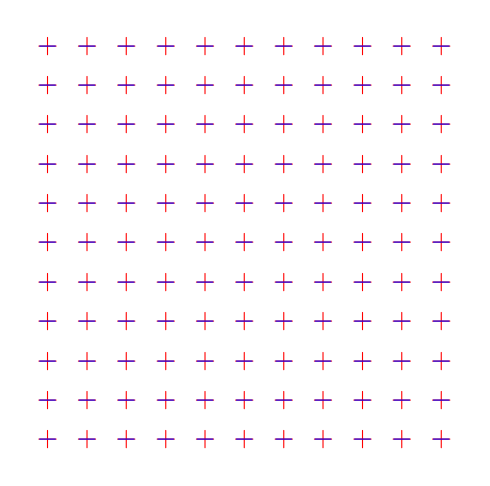
\begin{tikzpicture}

          \foreach \y in {0,1,...,10}
          {
            \foreach \x in {0,1,...,10}
            {
              \pgfmathtruncatemacro{\xnegpos}{0.5*\x + 0.02};
              \pgfmathtruncatemacro{\ynegpos}{0.5*\y + 0.02};
              \node[red] at (0.5*\x,0.5*\y) {$+$};
              \node[blue] at (0.5*\x,0.5*\y) {$-$};
            }
          }

         \end{tikzpicture}
         \caption{No induction, where $-$ is over $+$.}
         \label{fig:y equals x}
     \end{subfigure}
     \hfill
     \begin{subfigure}[b]{0.4\textwidth}
         \centering
          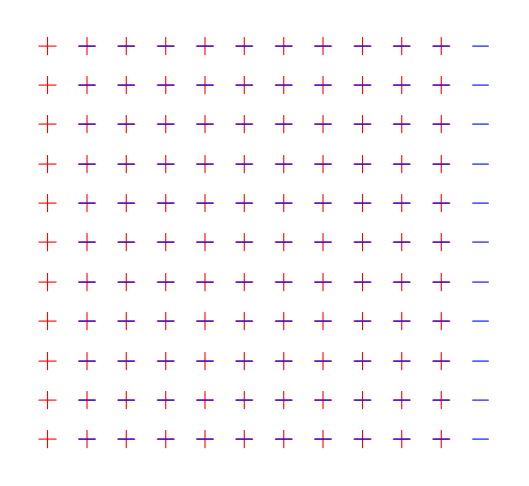
\begin{tikzpicture}


          \foreach \y in {0,...,10}
          {
            \foreach \x in {0,...,10}
            {
              \node[red] at (0.5*\x,0.5*\y) {$+$};
            }
            \foreach \x in {1,...,11}
            {
              \node[blue] at (0.5*\x,0.5*\y) {$-$};
            }
          }


         \end{tikzpicture}
         \caption{Induction, where $-$ is shifted to the right.}
         \label{fig:three sin x}
     \end{subfigure}
        \caption{No induction compared to induction.}
        \label{fig:three graphs}
\end{figure}

\section{Coulomb's Law}
\subsection{Electric Forces and Coulomb's Law}
%31:50 Coulomb's Law 
%40:00 what holds the world together, the autom scale the neculer force, then the electric force and on the size of planets and galixies it is the gravitational force. why
Coulomb's law describes the force resulted by two charged points $q_1$ and $q_2$, separated by a distance $r$ in vacuum.
\begin{equation}
  \vec{\boldsymbol{F}}_{12} = k_e \frac{q_1q_2}{r^2}\hat{\boldsymbol{r}}
\end{equation}
where $k_e$ is Coulomb's constant. The director $\hat{\boldsymbol{r}}$ is the unit vector directed from $q_1$ and $q_2$ defined as $\hat{\boldsymbol{r}}=\vec{\boldsymbol{r}}/r$. The direction of the force is determined by the sign of $q_1q_2\hat{\boldsymbol{r}}$, $(+)(+)=$ the same direction of $\hat{\boldsymbol{r}}$, $(-)(-)=$ same direction, $(+)(-)=$ opposite direction, and $(-)(+)=$ opposite direction.
See Figure~\ref{fig:coulomb-illustration} for the illustration of Coulomb's law.

\begin{figure}[H]
\centering
     \centering
     \begin{subfigure}[b]{0.45\textwidth}
         \centering
  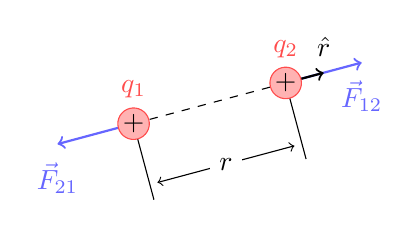
\begin{tikzpicture}

	\begin{scope}[rotate=15] 
    \draw[thick, blue!60, ->] (0,0) -- (-1,0) node[below=1mm] {$\vec{\boldsymbol{F}}_{21}$};  
    \draw[thick, blue!60, ->] (2,0) -- (3,0) node[below=1mm] {$\vec{\boldsymbol{F}}_{12}$}; 
    \draw[thick, ->] (2,0) -- (2.5,0) node[above=0.8mm] {$\hat{\boldsymbol{r}}$}; 

    \draw[dashed] (0,0) -- (2,0); 
    \draw (0,0) -- (0,-1);
    \draw (2,0) -- (2,-1);
    \draw[<->](0.1,-0.8)--(1.9,-0.8) node[midway,fill=white]{$r$};

    \filldraw[color=red!70, fill=red!30] (0,0) circle (2mm) node[above=2mm] {$q_1$};
    \node at (0,0) {$+$}; 
    \filldraw[color=red!70, fill=red!30] (2,0) circle (2mm) node[above=2mm] {$q_2$};
    \node at (2,0) {$+$}; 
  \end{scope}

	\end{tikzpicture}
       \caption{Repel (P - P).}
  \label{fig:coulomb-illustration-repel-p-p}
  \end{subfigure}
     \hfill
  \begin{subfigure}[b]{0.45\textwidth}
    \centering
  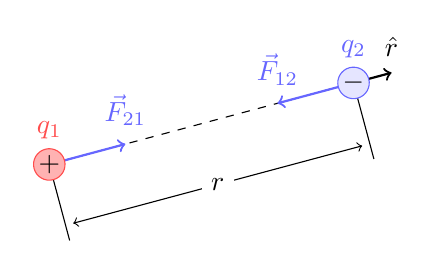
\begin{tikzpicture}

	\begin{scope}[rotate=15] 
    \draw[dashed] (0,0) -- (4,0); 
    \draw (0,0) -- (0,-1);
    \draw (4,0) -- (4,-1);
    \draw[<->](0.1,-0.8)--(3.9,-0.8) node[midway,fill=white]{$r$};
    \draw[thick, ->] (4,0) -- (4.5,0) node[above=0.8mm] {$\hat{\boldsymbol{r}}$}; 

    \draw[thick, blue!60, ->] (0,0) -- (1,0) node[above=1mm] {$\vec{\boldsymbol{F}}_{21}$};  
    \draw[thick, blue!60, ->] (4,0) -- (3,0) node[above=1mm] {$\vec{\boldsymbol{F}}_{12}$}; 


    \filldraw[color=red!70, fill=red!30] (0,0) circle (2mm) node[above=2mm] {$q_1$};
    \node at (0,0) {$+$}; 
    \filldraw[color=blue!60, fill=blue!10] (4,0) circle (2mm) node[above=2mm] {$q_2$};
    \node at (4,0) {$-$}; 
  \end{scope}

	\end{tikzpicture}
  \caption{Attracted (P - N).}
  \label{fig:coulomb-illustration-attracted-p-n}
  \end{subfigure}
\begin{subfigure}[b]{0.45\textwidth}
    \centering
  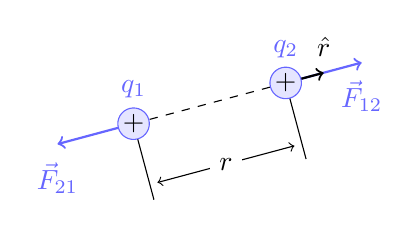
\begin{tikzpicture}

	\begin{scope}[rotate=15] 
    \draw[thick, blue!60, ->] (0,0) -- (-1,0) node[below=1mm] {$\vec{\boldsymbol{F}}_{21}$};  
    \draw[thick, blue!60, ->] (2,0) -- (3,0) node[below=1mm] {$\vec{\boldsymbol{F}}_{12}$}; 
    \draw[thick, ->] (2,0) -- (2.5,0) node[above=0.8mm] {$\hat{\boldsymbol{r}}$}; 

    \draw[dashed] (0,0) -- (2,0); 
    \draw (0,0) -- (0,-1);
    \draw (2,0) -- (2,-1);
    \draw[<->](0.1,-0.8)--(1.9,-0.8) node[midway,fill=white]{$r$};

    \filldraw[color=blue!60, fill=blue!10] (0,0) circle (2mm) node[above=2mm] {$q_1$};
    \node at (0,0) {$+$}; 
    \filldraw[color=blue!60, fill=blue!10] (2,0) circle (2mm) node[above=2mm] {$q_2$};
    \node at (2,0) {$+$}; 
  \end{scope}

	\end{tikzpicture}
  \caption{Repel (N - N).}
  \label{fig:coulomb-illustration-repel-n-n}
  \end{subfigure}
     \hfill
  \begin{subfigure}[b]{0.45\textwidth}
    \centering
  \begin{tikzpicture}

	\begin{scope}[rotate=15] 
    \draw[dashed] (0,0) -- (4,0); 
    \draw (0,0) -- (0,-1);
    \draw (4,0) -- (4,-1);
    \draw[<->](0.1,-0.8)--(3.9,-0.8) node[midway,fill=white]{$r$};
    \draw[thick, ->] (4,0) -- (4.5,0) node[above=0.8mm] {$\hat{\boldsymbol{r}}$}; 

    \draw[thick, blue!60, ->] (0,0) -- (1,0) node[above=1mm] {$\vec{\boldsymbol{F}}_{21}$};  
    \draw[thick, blue!60, ->] (4,0) -- (3,0) node[above=1mm] {$\vec{\boldsymbol{F}}_{12}$}; 


    \filldraw[color=blue!60, fill=blue!10] (0,0) circle (2mm) node[above=2mm] {$q_1$};
    \node at (0,0) {$-$}; 
    \filldraw[color=red!70, fill=red!30] (4,0) circle (2mm) node[above=2mm] {$q_2$};
    \node at (4,0) {$+$}; 
  \end{scope}

	\end{tikzpicture}
  \caption{Attracted (N - P).}
  \label{fig:coulomb-illustration-attracted-n-p}
  \end{subfigure}

  \caption{Illustration of Coulomb's Law.}
  \label{fig:coulomb-illustration}

\end{figure}


Coulomb's constant $k_e$ is defined as:
\begin{equation*}
  k_e = \frac{1}{4\pi\varepsilon_0} = \SI[per-mode = fraction]{8.9875e9}{\newton\meter\squared\per\coulomb\squared}
\end{equation*}
where $\varepsilon_0$ is the \textbf{Vacuum Permittivity}, also known as the
\textbf{Electric Constant} or the \textbf{Permittivity of Free Space}, i.e., a
measure of how much resistance the vacuum of empty space puts up against an
electric field.
\begin{equation*}
  \varepsilon_0 = \SI[per-mode = fraction]{8.85e-12}{\coulomb\squared\per\newton\meter\squared}
\end{equation*}


\section{Principle of Superposition}
Coulomb's laws applies to a pair of charged points and when there are more than
two charged points the net force on any charged point is the vector sum of all
forces exerted on it by the other changed points. 
\begin{equation*}
  \vec{\boldsymbol{F}}_{j} = \sum_{\substack{i=1 \\ j \neq i}}^{N} \vec{\boldsymbol{F}}_{ij}
\end{equation*}
where $\vec{\boldsymbol{F}}_{ij}$ denotes the force between charged point $i$ and $j$ for a system of $N$ charges.

\paragraph{Example:}
There are three charged points shown in Figure~\ref{fig:system-of-three-charges}. Find the force on charge $q_3$, when $q_1 = \SI{6.0e-6}{\coulomb}$, $q_2 = -q_1 = \SI{-6.0e-6}{\coulomb}$, $q_3 = \SI{3.0e-6}{\coulomb}$, and $\SI{2.0e-2}{\meter}$.

\begin{figure}[H]
\centering
\begin{tikzpicture}

  \draw (0,0) -- (0,4) node[above] {$y$} node[pos=0.4, left] {$a$};
  \draw (0,0) -- (4,0) node[right] {$x$};
  \draw[dashed] (0,0) -- (3,3) node[midway, below] {$\sqrt{2}a$};
  \draw[dashed] (3,3) -- (5,3);
  \draw (0,3) -- (3,3);
  \draw[dashed] (0.5,3) -- (1.5,4);
  \draw[dashed] (1.5,4) -- (4,4);
  \draw[thick] (1,0) arc[start angle=0, end angle=45, radius=10mm] node[midway, right] {$\theta$};
  \draw[thick, dashed, -Stealth] (4.5,3) arc[start angle=45, end angle=110, radius=20mm] node[midway, right=3mm] {$\phi$};

  \draw[color=blue!60, very thick, -Stealth] (3,3) -- (0.5,3) node[below] {$\vec{\boldsymbol{F}}_{23}$};
  \draw[color=blue!60, very thick, -Stealth] (3,3) -- (1.5,4) node[above] {$\vec{\boldsymbol{F}}_{3}$};
  \draw[color=blue!60, very thick, -Stealth] (3,3) -- (4,4) node[above right] {$\vec{\boldsymbol{F}}_{13}$};

  \draw[very thick, -Stealth] (3,3) -- (3.5,3.5) node[below right=0.5mm] {$\hat{\boldsymbol{r}}_{13}$};;
  \draw[very thick, -Stealth] (3,3) -- (3.8,3) node[below] {$\hat{\boldsymbol{r}}_{23}$};

  \filldraw[color=red!70, fill=red!30] (0,0) circle (2mm) node[left=2mm] {$q_1$};
  \node at (0,0) {$+$}; 
  \filldraw[color=blue!60, fill=blue!10] (0,3) circle (2mm) node[left=2mm] {$q_2$};
  \node at (0,3) {$-$}; 
  \filldraw[color=red!70, fill=red!30] (3,3) circle (2mm) node[below=2mm] {$q_3$};
  \node at (3,3) {$+$}; 

\end{tikzpicture}
  \caption{A system of three charges.}
  \label{fig:system-of-three-charges}
\end{figure}


\subparagraph{Solution:}
Using the super position principle, the force on $q_3$ is
\begin{equation*}
  \vec{\boldsymbol{F}}_{3} = \vec{\boldsymbol{F}}_{13} +
  \vec{\boldsymbol{F}}_{23} = \frac{1}{4\pi\varepsilon_0} \left(
  \frac{q_1q_3}{r^2_{13}}\hat{\boldsymbol{r}}_{13} + \frac{q_2q_3}{r^2_{23}}\hat{\boldsymbol{r}}_{23} \right)
\end{equation*}
where the unit vector $\hat{\boldsymbol{r}}_{13}$ is 
\begin{equation*}
  \hat{\boldsymbol{r}}_{13} = \cos{\theta}\hat{\boldsymbol{i}} + \cos{\theta}\hat{\boldsymbol{j}} = \frac{\sqrt{2}}{2}(\hat{\boldsymbol{i}} + \hat{\boldsymbol{j}})
\end{equation*}
and $\hat{\boldsymbol{r}}_{23} = \hat{\boldsymbol{i}}$. Therefore, the total force is 
\begin{align*}
  \vec{\boldsymbol{F}}_{3} &= \frac{1}{4\pi\varepsilon_0} \left(
  \frac{q_1q_3}{r^2_{13}}\hat{\boldsymbol{r}}_{13} + \frac{q_2q_3}{r^2_{23}}\hat{\boldsymbol{r}}_{23} \right)
  = \frac{1}{4\pi\varepsilon_0} \left(
  \frac{q_1q_3}{(\sqrt{2}a)^2}\frac{\sqrt{2}}{2}(\hat{\boldsymbol{i}} + \hat{\boldsymbol{j}}) 
  + \frac{(-q_1)q_3}{a^2}\hat{\boldsymbol{i}} \right) \\
  &= \frac{1}{4\pi\varepsilon_0} \frac{q_1q_3}{a^2} \left(\left(
  \frac{\sqrt{2}}{4}-1\right)\hat{\boldsymbol{i}} + \frac{\sqrt{2}}{4}\hat{\boldsymbol{j}} \right) 
\end{align*}
The total force, i.e., the ``length'' of the vector, can be calculated by pythagorean theorem $c=\sqrt{a^2+b^2}$, which gives us
\begin{align*}
  \vec{\boldsymbol{F}}_{3} 
  &= \frac{1}{4\pi\varepsilon_0} \frac{q_1q_3}{a^2} \sqrt{\left(
  \frac{\sqrt{2}}{4}-1\right)^2 + \left(\frac{\sqrt{2}}{4}\right)^2 } \\
  &= \left(\SI[per-mode =
  fraction]{9.0e9}{\coulomb\squared\per\newton\meter\squared}\right)
  \frac{(\SI{6.0e-6}{\coulomb})(\SI{3.0e-6}{\coulomb})}{(\SI{2.0e-2}{\meter})^2}
  (0.74) = \SI{3.0}{\newton}
\end{align*}
The angle of the force from the x-axis is
\begin{equation*}
  \phi = \arctan{\left( \frac{F_{3,y}}{F_{3,x}} \right)}
  = \arctan{\left( \frac{\sqrt{2}/4}{-1+\sqrt{2}/4} \right)} = \SI{151.3}{\degree}
\end{equation*}



\section{Electric Fields}

An electric field $\vec{\boldsymbol{E}}$ is defined as the electric force per unit charge experienced by a small positive test charge placed at a point in space. The small positive test charge will be canceled out in the derivations so the actual value of test charge $q_0$ is not important, but we say that it is infinitesimally small.
\begin{equation*}
  \vec{\boldsymbol{E}} = \lim_{q_0\to0}\frac{\vec{\boldsymbol{F}}}{q_0}
\end{equation*}
And with Coulomb's law we get:
\begin{equation*}
  \vec{\boldsymbol{E}} = \frac{1}{4\pi\varepsilon_0}\frac{Qq_0}{q_0r^2}\hat{\boldsymbol{r}} 
  = \frac{1}{4\pi\varepsilon_0}\frac{Q}{r^2}\hat{\boldsymbol{r}} 
\end{equation*}
Where $Q$ is a stationary charge.

Now for all charges in a given space $q_i$, we can use the super position principle and get the following electric fields:
\begin{equation*}
  \vec{\boldsymbol{E}} = \sum_i\vec{\boldsymbol{E}}_i = \sum_i\frac{1}{4\pi\varepsilon_0}\frac{q_i}{r^2}\hat{\boldsymbol{r}} 
\end{equation*}


\subsection{Electric Fields Lines}
A convenient way of representing the electric fields are with electric field lines.
\begin{figure}[H]
\centering
  \begin{subfigure}[b]{0.45\textwidth}
    \centering
\begin{tikzpicture}[
    scale=0.80,
    attach arrow/.style args={#1}{
        decoration={
            markings,
            mark=at position 0 with {\pgfextra{%
                \pgfmathsetmacro{\tmpArrowTime}{\pgfkeysvalueof{/tikz/arc arrow/length}/(\pgfdecoratedpathlength)}%
                \xdef\tmpArrowTime{\tmpArrowTime}}},
            mark=at position {#1-3*\tmpArrowTime} with {\coordinate(@1);},
            mark=at position {#1-2*\tmpArrowTime} with {\coordinate(@2);},
            mark=at position {#1-1*\tmpArrowTime} with {\coordinate(@3);},
            mark=at position {#1+\tmpArrowTime/2} with {\coordinate(@4);
                \draw[-{Stealth[length=\pgfkeysvalueof{/tikz/arc arrow/length},bend]}]
                  plot[smooth] coordinates {(@1) (@2) (@3) (@4)};},
        },
        postaction=decorate,
    },
    attach arrow/.default=0.5,
    arc arrow/.cd, length/.initial=2mm,
]
\node[draw=red!70, fill=red!30, circle, minimum size=6mm] (Q) {+};

% Radial outward field lines
\foreach \a in {0,30,...,330} {
  \draw[red!70, thick, attach arrow={1/3}, attach arrow={2/3}] (Q) -- ++(\a:3);
}
\end{tikzpicture}
  \caption{}
  \label{fig:electric-field-line-for-positive}
  \end{subfigure}
     \hfill
  \begin{subfigure}[b]{0.45\textwidth}
    \centering
\begin{tikzpicture}[
    scale=0.80,
    attach arrow/.style args={#1}{
        decoration={
            markings,
            mark=at position 0 with {\pgfextra{%
                \pgfmathsetmacro{\tmpArrowTime}{\pgfkeysvalueof{/tikz/arc arrow/length}/(\pgfdecoratedpathlength)}%
                \xdef\tmpArrowTime{\tmpArrowTime}}},
            mark=at position {#1-3*\tmpArrowTime} with {\coordinate(@1);},
            mark=at position {#1-2*\tmpArrowTime} with {\coordinate(@2);},
            mark=at position {#1-1*\tmpArrowTime} with {\coordinate(@3);},
            mark=at position {#1+\tmpArrowTime/2} with {\coordinate(@4);
                \draw[-{Stealth[length=\pgfkeysvalueof{/tikz/arc arrow/length},bend]}]
                  plot[smooth] coordinates {(@1) (@2) (@3) (@4)};},
        },
        postaction=decorate,
    },
    attach arrow/.default=0.5,
    arc arrow/.cd, length/.initial=2mm,
]
\node[draw=blue!70, fill=blue!20, circle, minimum size=6mm] (Q) {$-$};

% Radial inward field lines
\foreach \a in {0,30,...,330} {
  \draw[red!70, thick, attach arrow={1/3}, attach arrow={2/3}] ++(\a:3) -- (Q);
}
\end{tikzpicture}
  \caption{}
  \label{fig:electric-field-line-negative}
  \end{subfigure}
  \caption{Field lines for (a) positive, radially outwards, and (b) negative charges, radially inwards.}
  \label{fig:electric-field-lines}
\end{figure}


\begin{figure}[H]
\centering
\begin{tikzpicture}[
    scale=1,
    attach arrow/.style={
        decoration={
            markings,
            mark=at position 0 with {\pgfextra{%
                \pgfmathsetmacro{\tmpArrowTime}{\pgfkeysvalueof{/tikz/arc arrow/length}/(\pgfdecoratedpathlength)}%
                \xdef\tmpArrowTime{\tmpArrowTime}}},
            mark=at position {#1-3*\tmpArrowTime} with {\coordinate(@1);},
            mark=at position {#1-2*\tmpArrowTime} with {\coordinate(@2);},
            mark=at position {#1-1*\tmpArrowTime} with {\coordinate(@3);},
            mark=at position {#1+\tmpArrowTime/2} with {\coordinate(@4);
                \draw[-{Stealth[length=\pgfkeysvalueof{/tikz/arc arrow/length},bend]}] plot[smooth]
                coordinates {(@1) (@2) (@3) (@4)};},
        },
        postaction=decorate,
    },
    attach arrow/.default=0.5,
    arc arrow/.cd,length/.initial=2mm,
    %nodes={circle,minimum size=2.4em,font=\bfseries\sffamily}
]
\path 
    node[draw=red!70, fill=red!30, circle, minimum size=6mm] (L){+} 
    (2.5,0) node[draw=blue!60, fill=blue!10, circle, minimum size=6mm] (R){--};
\foreach \X in {0,...,7}
 {\draw[red!70, thick, attach arrow] (L) 
 to[bend left={-70+\X*20},looseness=1.6] 
 (R);}
\foreach \X in {0,...,10}
 {\draw[red!70, thick,attach arrow/.list={1/3,2/3}] (L) to[bend left=16-4*\X] ++ (70+\X*22:3);
 \draw[red!70, thick,attach arrow/.list={1/3,2/3}] (R)+(180+70+\X*22:3) 
 to[bend right=16-4*\X] 
  (R);}
\end{tikzpicture}
  \caption{Field lines for an electric dipole.}
  \label{fig:electric-field-line-for-dipole}
\end{figure}


\subsection{Force Exerted on a Charged Particle in a Constant Electric Field}
Consider a charged particle $+q$ in an electric field formed by a positive and negative infinitely large source plates, as shown in Figure~\ref{fig:electric-field-of-source-plates}. 
\begin{figure}[H]
\centering
\begin{tikzpicture}
  \filldraw[color=red!70, fill=red!30] (0,3.5) rectangle (7,3.9);
  \filldraw[color=blue!60, fill=blue!10] (0,0) rectangle (7,0.4);
  \foreach \x in {0,...,6} {
	  \node at (\x+0.5,3.7) {$+$};
	  \node at (\x+0.5,0.2) {$-$};
  }
  \draw[<->] (0.2,0.4) -- (0.2,3.5) node[midway, fill=white] {$y$};
  \draw[red!70, ->] (6.8,3.5) -- (6.8,0.4) node[midway, right] {$\vec{\boldsymbol{E}}$};
  \draw[dashed] (3.5,3) -- (3.5,0.9);

  \filldraw[dotted, very thick, color=red!70, fill=white] (3.5,3) circle (2mm) node[right=2mm] {$q$};
  \filldraw[color=red!70, fill=red!30] (3.5,0.9) circle (2mm);

	\node at (2.5,2.8) {$\vec{\boldsymbol{V}}=\vec{\boldsymbol{0}}$};
  \draw[thick, -Stealth] (4,1.3) -- (4,0.6) node[midway, right] {$\vec{\boldsymbol{V}}$};

\end{tikzpicture}
  \caption{A charge $q$ moving in a constant electric field formed by two infinity large source plates.}
  \label{fig:electric-field-of-source-plates}
\end{figure}

The electric field between the source plates is $\vec{\boldsymbol{E}}=-E_y\hat{\boldsymbol{j}}$, with $E_y>0$. The charge $q$ will experience a downward force
\begin{equation*}
  \vec{\boldsymbol{F}}_e = q \vec{\boldsymbol{E}}
\end{equation*}

With Newton's Second Law $F=ma$, the net force will cause the charge to accelerate with an acceleration
\begin{equation*}
  \vec{\boldsymbol{a}} = \frac{\vec{\boldsymbol{F}}_e}{m} = \frac{q\vec{\boldsymbol{E}}}{m}
  = -\frac{qE_y}{m}\hat{\boldsymbol{j}}
\end{equation*}

Remember that the standard kinematics is described as $v_f^2=v_i^2+2ad$, where $v_f$ is the final velocity and $v_i$ is the initial velocity. The final velocity of the particle hitting the negative charged plate is therefore:
\begin{equation*}
  v_y = \sqrt{2|a_y|y} = \sqrt{\frac{2yqE_y}{m}}
\end{equation*}

Thus, the kinetic energy of the particle when it hits the plate is:
\begin{equation*}
  K = \frac{1}{2}mv_y^2 = qE_yy
\end{equation*}




% TODO: calculation of electric field of a dipole
% TODO: calculation of tourque of a dipole
% TODO: potential energy of a dipole
% TODO: charge density



\section{Electric Potential}
Electric potential energy is similar to gravitational potential energy. A mass higher up has more potential energy, just like a charge closer to a source charge has more electrical potential energy.

The electric potential (measured in Volts) is the potential energy per unit charge. This is analogous to height in gravity. The height of a cliff is the same for a tennis ball or a gold ball; it's a property of the location. Similarly, electric potential is a property of the point in space, set by the source charge, independent of any test charge placed there.
\begin{equation*}
  V=\frac{U}{q}
\end{equation*}
where $V$ is the electric potential defined in Volts $(\si{\volt})$, $U$ is the electric potential energy defined in Joules $(\si{\joule})$, and $q$ is the charge defined in Coulombs $(\si{\coulomb})$.
However, a more useful scale for electric potential is the energy acquires/losses when moving through a potential difference of one volt, we denote it as $(\si{\electronvolt})$.

Similar to gravity where the negative work done, i.e.,
\begin{equation*}
  \Delta V_g = \frac{\Delta U_g}{m} = -\int_A^B(\vec{\boldsymbol{F}}_g/m)\cdot d\vec{\boldsymbol{s}} = - \int_A^B\vec{\boldsymbol{g}}\cdot d\vec{\boldsymbol{s}},
\end{equation*}
the electric potential difference between two points $A$ and $B$ is 
\begin{equation}\label{eq:electric-potential-difference}
  \Delta V = -\int_A^B(\vec{\boldsymbol{F}}_e/q_0)\cdot d\vec{\boldsymbol{s}} = -\int_A^B\vec{\boldsymbol{E}}\cdot d\vec{\boldsymbol{s}}
\end{equation}
where $d\vec{\boldsymbol{s}}$ is the vector in from $A$ to $B$.


\subsection{Electric Potential in a Uniform Field}
Consider a positive charge $+q$ moving in the direction of a uniform electric field $\vec{\boldsymbol{E}} = E_0(-\hat{\boldsymbol{j}})$, as shown in Figure~\ref{fig:charge-moving-in-a-uniform-electric-field}.

\begin{figure}[H]
\centering
\begin{tikzpicture}
  \node[circle, draw=red!70, very thick, dotted, minimum size=2mm, text=black] (start) at (1,4) {$+$};
  \node[circle, draw=red!70, fill=red!30, minimum size=2mm, text=black] (end) at (1,2) {$+$};
  \draw[dashed] (start) -- (end);
  \draw[thick] (start) -- ++(1,0);
  \draw[thick] (end) -- ++(1,0);
  \draw[thick, latex-latex] ([xshift=5mm]start.east) -- ([xshift=5mm]end.east) node[midway, fill=white] {$d$};
  \node at ([xshift=-2mm]start.west) {$A$};
  \node at ([xshift=-2mm]end.west) {$B$};
  \node at ([xshift=1.8mm,yshift=1.5mm]end.north) {$q$};

  \node at (0, 1) {$\vec{\boldsymbol{E}}$};
	\begin{scope}[xshift=4mm] 
    \foreach \x in {0,1,...,5} {
      \draw[-latex, thick, red!70] (\x*0.4, 1.5) -- (\x*0.4, 0);
    }
	\end{scope}

\end{tikzpicture}
  \caption{A charge $q$ moving in a uniform electric field}
  \label{fig:charge-moving-in-a-uniform-electric-field}
\end{figure}

The potential difference between point $A$ and $B$ is
\begin{equation*}
  \Delta V = V_B - V_A = -\int_A^B \vec{\boldsymbol{E}} \cdot d\vec{\boldsymbol{s}} = -E_0\int_A^B ds = -E_0d < 0
\end{equation*}
Since $-E_0d < 0$, $B$ has a lower electric potential than $A$. The electric field lines indicate where the electric potential is higher, since the lines points from higher potential to lower.

Figure~\ref{fig:potantial-difference-in-a-uniform-electric-field} illustrates the difference in electric potential between two points $A$ and $B$ where they are not parallel to the electric field $\vec{\boldsymbol{E}}$.
\begin{figure}[H]
\centering
\begin{tikzpicture}

  \node at (3, 0.6) {$\vec{\boldsymbol{E}}$};
	\begin{scope}[xshift=4mm] 
    \foreach \x in {0,1,...,5} {
      \draw[-latex, thick, red!70] (\x*0.5, 4) -- (\x*0.5, 0);
    }
	\end{scope}

  \node[circle, fill, inner sep=1.2pt] (A) at (1.2,3.5) {};
  \node[circle, fill, inner sep=1.2pt] (B) at (2.2,0.7) {};
  \node[circle, fill, inner sep=1.2pt] (C) at (1.2,0.7) {};

  \draw ([yshift=-7mm]A.south) arc[start angle=-90, end angle=-70, radius=7mm] node[midway, below] {\small $\theta$};

  \draw[very thick, -latex] (A) -- (B) node[midway, right=1mm] {$\vec{\boldsymbol{s}}$};
  \draw[thick, dashed] (A) -- (C);
  \draw[thick, dashed] (C) -- (B);

  \node[above] at (A) {$A$};
  \node[below] at (B) {$B$};
  \node[below] at (C) {$C$};

	\draw[decorate, decoration={brace, mirror, amplitude=3mm}] (A.west) -- (C.west) node[midway, left=3mm] {\small $y$};

\end{tikzpicture}
  \caption{Potential difference between two points in a uniform electric field}
  \label{fig:potantial-difference-in-a-uniform-electric-field}
\end{figure}
The difference in electric potential between $C$ and $B$ is zero, since the path is perpendicular to the electric field. Thus, the difference in electric potential does not depend on the angle $\theta$, only the distance between $A$ and $C$, i.e., $y$.

\begin{align*}
  \Delta V &= V_B - V_A = \Delta V_{CA} + \Delta V_{BC} = \Delta V_{CA} \\
  &= -\int_A^B \vec{\boldsymbol{E}} \cdot d\vec{\boldsymbol{s}} = -E_0s\cos{\theta} = -E_0y
\end{align*}


\subsection{Electric Potential due to a Point Charge}
Consider a point charge $Q$. The field produced by $Q$ is $\vec{\boldsymbol{E}}=(Q/4\pi\varepsilon_0r^2)\hat{\boldsymbol{r}}$. From Figure~\ref{fig:potantial-difference-due-to-point-charge} we see that $\hat{\boldsymbol{r}}d\vec{\boldsymbol{s}}=ds\cos{\theta}=dr$. The electric potential difference between two points $A$ and $B$ is therefor
\begin{equation*}
  \Delta V = V_B - V_A = -\int_A^B\frac{Q}{4\pi\varepsilon_0r^2}\hat{\boldsymbol{r}}d\vec{\boldsymbol{s}} = -\int_A^B\frac{Q}{4\pi\varepsilon_0r^2}dr = \frac{Q}{4\pi\varepsilon_0}\left( \frac{1}{r_B} - \frac{1}{r_A} \right)
\end{equation*}

\begin{figure}[H]
\centering
\begin{tikzpicture}

  \coordinate (CQ) at (0, 0);
  \coordinate (CA) at ({sin(-15)*2}, {cos(15)*2});
  \coordinate (CB) at ({sin(70)*4}, {cos(70)*4});
  \coordinate (CR) at ({sin(30)*2.5}, {cos(30)*2.5});

  \node[circle, fill=red!70, inner sep=1.2pt] (Q) at (CQ) {};
  \node[below] at (Q) {$Q$};

  \draw[dashed, blue!30] ([xshift=2cm]Q) arc[start angle=0, end angle=120, radius=2cm];
  \draw[dashed, blue!30] ([xshift=4cm]Q) arc[start angle=0, end angle=120, radius=4cm];

  \node[circle, fill, inner sep=1.2pt] (A) at (CA) {};
  \node[circle, fill, inner sep=1.2pt] (B) at (CB) {};

  \draw[orange!70] (A) to[out=30, in=160] (CR) to[out=-20, in=150] (B);

  \node[above] at (A) {$A$};
  \node[right] at (B) {$B$};

  \draw[thick, -latex] (Q) -- (A) node[midway, left] {$\vec{\boldsymbol{r}}_A$};
  \draw[thick, -latex] (Q) -- (B) node[midway, below] {$\vec{\boldsymbol{r}}_B$};
  \draw[thick, -latex] (Q) -- (CR) node[midway, right] {$\vec{\boldsymbol{r}}$};
  \draw[thick, -latex, blue!60] (CR) -- ($(CR)!0.3!(B)$) node[below] {$d\vec{\boldsymbol{s}}$};
  \draw[thick, -latex, blue!60] (Q) -- ($(Q)!0.3!(CR)$) node[midway, right] {$\hat{\boldsymbol{r}}$};
  \draw[thin] (Q) -- ($(Q)!1.3!(CR)$);
  \draw[thin, dashed] ($(Q)!1.1!(CR)$) -- ($(CR)!0.3!(B)$);

	\draw[decorate, decoration={brace, mirror, amplitude=1mm}] ($(Q)!1.1!(CR)$) -- (CR)  node[near start, left] {\small $dr$};
  \draw ($(CR)!0.07!(B)$) arc[start angle=-20, end angle=70, radius=2mm] coordinate[midway] (midarc); 
  \draw (midarc) -- ++(0.5, 0.2) node[right] {\small $\theta$};
  

\end{tikzpicture}
  \caption{Potential difference between two points due to a point charge.}
  \label{fig:potantial-difference-due-to-point-charge}
\end{figure}


\subsection{Potential Energy in a System of Charges}
Imagine a system of charges is assembled by an external agent. If there is only one charge no work is node $W_1=0$. If the external agent brings a second charge in the system the work done is $W_2=q_2V_1$. Generally the work done is $W_{\text{ext}}=\Delta U$, i.e., the work the external agent has to do is the change in the systems potential energy. For two charges it is
\begin{equation*}
  U_{1\,2} = W_2 = \frac{1}{4\pi\varepsilon_0}\frac{q_1q_2}{r_{1\,2}}
\end{equation*}
And if the external agent brings a third charge the work done for charge $q_3$ is will be
\begin{equation*}
  W_3 = q_3(V_1+V_2)=\frac{q_3}{4\pi\varepsilon_0}\left(\frac{q_1}{r_1\,r_3}+\frac{q_2}{r_{2\,3}}\right)
\end{equation*}
Thus the potential energy is the sum of the all work done
\begin{equation*}
  U = W_2 + W_3 = \frac{1}{4\pi\varepsilon_0}\left(\frac{q_1q_2}{r_{1\,2}}+\frac{q_1q_3}{r_{1\,3}}+\frac{q_2q_3}{r_{2\,3}}\right)
\end{equation*}
The general equation the total potential energy, i.e., work done by the external agent, of $N$ charges is
\begin{equation*}
  U = \frac{1}{4\pi\varepsilon_0} \sum_{i=1}^N\sum_{\substack{j=1 \\ j > i}}\frac{q_iq_j}{r_{i\,j}}
\end{equation*}

\subsection{Deriving Electric Fields from the Electric Potential}
% TODO: deriving electric fields from electric potential
Consider two points separated with a distance $d\vec{\boldsymbol{d}}$, by using Eq.~\ref{eq:electric-potential-difference} we can derive the following differential from:
\begin{equation*}
  dV = -\vec{\boldsymbol{E}}\cdot d\vec{\boldsymbol{s}}
\end{equation*}
In Cartesian coordinates, $\vec{\boldsymbol{E}}=E_x\hat{\boldsymbol{i}}+E_y\hat{\boldsymbol{j}}+E_z\hat{\boldsymbol{k}}$ and $d\vec{\boldsymbol{s}}=dx\hat{\boldsymbol{i}}+dy\hat{\boldsymbol{j}}+dz\hat{\boldsymbol{k}}$, we have
\begin{equation*}
  dV = \left(E_x\hat{\boldsymbol{i}}+E_y\hat{\boldsymbol{j}}+E_z\hat{\boldsymbol{k}}\right)\cdot\left(dx\hat{\boldsymbol{i}}+dy\hat{\boldsymbol{j}}+dz\hat{\boldsymbol{k}}\right) = E_xdx + E_ydy + E_zdz
\end{equation*}
which implies
\begin{equation*}
  E_x = -\frac{\partial V}{\partial x},\: E_y = -\frac{\partial V}{\partial y},\: E_z = -\frac{\partial V}{\partial z}
\end{equation*}
We now introduce a differential quantity called the ``del (gradient) operator'' to simplifiy the notation.
\begin{equation*}
  \nabla \equiv \frac{\partial}{\partial x} \hat{\boldsymbol{i}} + \frac{\partial}{\partial y} \hat{\boldsymbol{j}} + \frac{\partial}{\partial z} \hat{\boldsymbol{k}} 
\end{equation*}
We then get 
\begin{equation*}
  \vec{\boldsymbol{E}} =  E_x\hat{\boldsymbol{i}} + E_y\hat{\boldsymbol{j}} + E_z\hat{\boldsymbol{k}}
-\left(\frac{\partial V}{\partial x} \hat{\boldsymbol{i}} + \frac{\partial V}{\partial y} \hat{\boldsymbol{j}} + \frac{\partial V}{\partial z} \hat{\boldsymbol{k}}\right)
  = 
  \left(\frac{\partial}{\partial x} \hat{\boldsymbol{i}} + \frac{\partial}{\partial y} \hat{\boldsymbol{j}} + \frac{\partial}{\partial z} \hat{\boldsymbol{k}}\right)V = -\nabla V
\end{equation*}

\begin{equation}\label{eq:electric-field-del-gradient-potential}
  \vec{\boldsymbol{E}} = -\nabla V
\end{equation}

If the charges in the system is having a spherical electric field, the electric field is a function of the radial distance $r$, i.e., $\vec{\boldsymbol{E_r}}=E_r\hat{\boldsymbol{r}}$, when $dV = -E_r dr$. If $V(r)$ the electric field can then be obtained
\begin{equation*}
  \vec{\boldsymbol{E}} = E_r\hat{\boldsymbol{r}} = -\left( \frac{dV}{dr} \right)\hat{\boldsymbol{r}}
\end{equation*}
For instance, electric potential due to a point charge's electric field can be calculated as $V(r)=q/4\pi\varepsilon_0 r$. Thus, the electric field produced is $\vec{\boldsymbol{E}}=(q/4\pi\varepsilon_0 r^2)\hat{\boldsymbol{r}}$.



\subsection{Gradient and Equipotentials}
% TODO: Graidiant and endpoints
%Eq.~\ref{eq:electric-field-del-gradient-potential}

An equipotential curve shows the levels of electric potential. The intersection of the equipotential curve and the electric field lines are always perpendicular, i.e., $\vec{\boldsymbol{E}} \perp d\vec{\boldsymbol{s}}$, shown in Figure~\ref{fig:equipotential-curves-and-electric-field-lines}. The difference in the electric potential between two levels of the equipotential curve is 
\begin{equation*}
  dV = \left( \frac{\partial V}{\partial x}\hat{\boldsymbol{i}} + \frac{\partial V}{\partial y}\hat{\boldsymbol{j}} \right)\cdot\left( dx\hat{\boldsymbol{i}} + dy\hat{\boldsymbol{j}} \right) = (\nabla)\cdot d\vec{\boldsymbol{s}} = -\vec{\boldsymbol{E}}\cdot d\vec{\boldsymbol{s}}
\end{equation*}

% Perpendicular
% Equipotetial cuervs


\begin{figure}[H]
\centering
\begin{subfigure}[b]{0.3\textwidth}
  \centering
\begin{tikzpicture}
  \foreach \d in {0,0.5,...,3.5} {
    \draw[red!70, -Stealth] (-0.2,\d) -- (3.8,\d);
    \draw[blue!60, dashed] (\d,-0.2) -- (\d,3.8);
  }
  \node at (4.1,3.3) {$\vec{\boldsymbol{E}}$};
\end{tikzpicture}
  \caption{} 
  %\label{fig:electric-field-line-for-positive} 
\end{subfigure}
    \hfill
\begin{subfigure}[b]{0.26\textwidth}
  \centering
\begin{tikzpicture}[
      scale=0.70,
      attach arrow/.style args={#1}{
          decoration={
              markings,
              mark=at position 0 with {\pgfextra{%
                  \pgfmathsetmacro{\tmpArrowTime}{\pgfkeysvalueof{/tikz/arc arrow/length}/(\pgfdecoratedpathlength)}%
                  \xdef\tmpArrowTime{\tmpArrowTime}}},
              mark=at position {#1-3*\tmpArrowTime} with {\coordinate(@1);},
              mark=at position {#1-2*\tmpArrowTime} with {\coordinate(@2);},
              mark=at position {#1-1*\tmpArrowTime} with {\coordinate(@3);},
              mark=at position {#1+\tmpArrowTime/2} with {\coordinate(@4);
                  \draw[-{Stealth[length=\pgfkeysvalueof{/tikz/arc arrow/length},bend]}]
                    plot[smooth] coordinates {(@1) (@2) (@3) (@4)};},
          },
          postaction=decorate,
      },
      attach arrow/.default=0.5,
      arc arrow/.cd, length/.initial=2mm,
  ]
  \node[draw=red!70, fill=red!30, circle, minimum size=6mm] (Q) {$+$};
  
  % Radial inward field lines
  \foreach \a in {0,30,...,330} {
    \draw[red!70, thick, attach arrow={1/2}] (Q) -- ++(\a:3);
  }
  \draw[blue!60, dashed] (L) circle (8mm);
  \draw[blue!60, dashed] (L) circle (14mm);
  \draw[blue!60, dashed] (L) circle (24mm);
\end{tikzpicture}
  \caption{}
  %\label{fig:electric-field-line-for-positive}
\end{subfigure}
    \hfill
\begin{subfigure}[b]{0.4\textwidth}
    \centering
\begin{tikzpicture}[
    scale=0.7,
    attach arrow/.style={
        decoration={
            markings,
            mark=at position 0 with {\pgfextra{%
                \pgfmathsetmacro{\tmpArrowTime}{\pgfkeysvalueof{/tikz/arc arrow/length}/(\pgfdecoratedpathlength)}%
                \xdef\tmpArrowTime{\tmpArrowTime}}},
            mark=at position {#1-3*\tmpArrowTime} with {\coordinate(@1);},
            mark=at position {#1-2*\tmpArrowTime} with {\coordinate(@2);},
            mark=at position {#1-1*\tmpArrowTime} with {\coordinate(@3);},
            mark=at position {#1+\tmpArrowTime/2} with {\coordinate(@4);
                \draw[-{Stealth[length=\pgfkeysvalueof{/tikz/arc arrow/length},bend]}] plot[smooth]
                coordinates {(@1) (@2) (@3) (@4)};},
        },
        postaction=decorate,
    },
    attach arrow/.default=0.5,
    arc arrow/.cd,length/.initial=2mm,
    %nodes={circle,minimum size=2.4em,font=\bfseries\sffamily}
]
  \path 
      node[draw=red!70, fill=red!30, circle, minimum size=4mm] (L){$+$} 
      (2.5,0) node[draw=blue!60, fill=blue!10, circle, minimum size=4mm] (R){$-$};
  \foreach \X in {0,...,4}
   {\draw[red!70, thick, attach arrow] (L) 
   to[bend left={-70+\X*35},looseness=1.6] 
   (R);}
  \foreach \X in {0,...,5}
   {\draw[red!70, thick,attach arrow/.list={1/2}] (L) to[bend left=16-8*\X] ++ (70+\X*44:3);
   \draw[red!70, thick,attach arrow/.list={1/2}] (R)+(180+70+\X*44:3) 
   to[bend right=16-8*\X] 
    (R);}
  \draw[blue!60, dashed] (L) ellipse (8mm and 7mm);
  \draw[blue!60, dashed] ([xshift=-1.4mm]L) ellipse (10mm and 9.5mm);
  \draw[blue!60, dashed] ([xshift=-3.6mm]L) circle (14mm);
  \draw[blue!60, dashed] ([xshift=-8.2mm]L) circle (20mm);
  \draw[blue!60, dashed] (1.2,-3) -- (1.2,3);
  \draw[blue!60, dashed] (R) ellipse (8mm and 7mm);
  \draw[blue!60, dashed] ([xshift=1.4mm]R) ellipse (10mm and 9.5mm);
  \draw[blue!60, dashed] ([xshift=3.6mm]R) circle (14mm);
  \draw[blue!60, dashed] ([xshift=8.2mm]R) circle (20mm);
\end{tikzpicture}
  \caption{}
  %\label{fig:electric-field-line-negative}
  \end{subfigure}
  \caption{A charge $q$ moving in a constant electric field formed by two infinity large source plates.}
  \label{fig:equipotential-curves-and-electric-field-lines}
\end{figure}





\section{Gauss' Law}
\section{Capacitors}
\section{Current and Resistance}
\section{Direct Current Circuits}
\section{Magnetic Fields}
\section{Sources of Magnetic Fields}
\section{Faraday's Law}
\section{Inductance and Energy in Magnetic Fields}
\section{Alternating Current Circuits}
\section{Maxwell's Equations and Electromagnetic Waves}
\section{Interference and Diffraction}


 \newpage
\newcommand{\pathPIII}{\pathPHY/Physics-III} \chapter{Physics III} \newpage

\newcommand{\pathCMII}{\pathPHY/Classical-Mechanics-II} \chapter{Classical Mechanics II}
This compendium is based on the book ``Intermediate Classical Mechanics'' by Professor Yih-Hsing Pao and Professor Li-Sheng Wang of Institute of Applied Mechanics, National Taiwan University from 2025~\cite{Pao2025Intermediate} and MIT OpenCourseWare ``Classical Mechanics II'' by professor Matthew Evans in 2017.
I can not guarantee the accuracy of this compendium and that it is a correct interpretation of the material and explanation provided by the lecture notes and lectures. Thus, for accurate information refer to the material that this compendium is based on. If a mistake is in the compendium it is most likely my fault and not the fault of the material in which this compendium is based on.
 \newpage
\newcommand{\pathCMIII}{\pathPHY/Classical-Mechanics-III} \chapter{Classical Mechanics III}
This compendium is based on the book ``Intermediate Classical Mechanics'' by Professor Yih-Hsing Pao and Professor Li-Sheng Wang of Institute of Applied Mechanics, National Taiwan University from 2025~\cite{Pao2025Intermediate}, it is also based on MIT OpenCourseWare ``Classical Mechanics III'' by Professor Iain Stewart and finally ``Port-Hamiltonian systems: an introductory survey'' by Professor Arjan van der Schaft~\cite{Port-HamiltonianAjal2006}.
I can not guarantee the accuracy of this compendium and that it is a correct interpretation of the material and explanation provided by the lecture notes and lectures. Thus, for accurate information refer to the material that this compendium is based on. If a mistake is in the compendium it is most likely my fault and not the fault of the material in which this compendium is based on.

\section{Hamiltonian mechanics}
\textbf{Hamiltonian mechanics} is a reformulation of classical mechanics that provides deep insights into both classical and quantum systems. It is named after the Irish mathematician William Rowan Hamilton and is built upon the concept of the \textit{Hamiltonian function}, which describes the total energy of the system.

Hamiltonian mechanics provides a bridge between classical mechanics and quantum mechanics and forms the foundation of many modern physical theories.

\section{Key Concepts}
\begin{itemize}
    \item \textbf{Phase Space:} A 2$n$-dimensional space where each point represents the state of the system, with generalized coordinates $q_i$ and conjugate momenta $p_i$.
    \item \textbf{Hamiltonian Function:} Denoted by $H(q_i, p_i, t)$, the Hamiltonian typically represents the total energy of the system (kinetic + potential energy).
    \item \textbf{Canonical Variables:} The generalized coordinates $q_i$ and conjugate momenta $p_i$ form pairs of canonical variables.
\end{itemize}

\section{Hamilton's Equations of Motion}
Hamilton's equations are a set of first-order differential equations that describe the time evolution of a system:
\[
\dot{q}_i = \frac{\partial H}{\partial p_i}, \quad \dot{p}_i = -\frac{\partial H}{\partial q_i}
\]
where:
\begin{itemize}
    \item $\dot{q}_i = \frac{dq_i}{dt}$ is the time derivative of the generalized coordinate.
    \item $\dot{p}_i = \frac{dp_i}{dt}$ is the time derivative of the conjugate momentum.
\end{itemize}

\section{Derivation from the Principle of Least Action}
Hamiltonian mechanics can be derived from the \textit{principle of least action}, where the action $S$ is given by:
\[
S = \int_{t_1}^{t_2} \left( \sum_{i=1}^{n} p_i \dot{q}_i - H \right) dt
\]
The equations of motion are obtained by requiring that $S$ be stationary ($\delta S = 0$).

\section{Examples}
\subsection*{1. Simple Harmonic Oscillator}
For a simple harmonic oscillator with mass $m$ and spring constant $k$, the Hamiltonian is:
\[
H = \frac{p^2}{2m} + \frac{1}{2} k q^2
\]
Hamilton's equations are:
\[
\dot{q} = \frac{\partial H}{\partial p} = \frac{p}{m}, \quad \dot{p} = -\frac{\partial H}{\partial q} = -kq
\]

\subsection{2. Free Particle}
For a free particle of mass $m$, the Hamiltonian is purely kinetic:
\[
H = \frac{p^2}{2m}
\]
The equations of motion are:
\[
\dot{q} = \frac{p}{m}, \quad \dot{p} = 0
\]

\section{Canonical Transformations}
A \textit{canonical transformation} preserves the form of Hamilton's equations. If $(q_i, p_i) \to (Q_i, P_i)$ is a transformation such that the new variables also satisfy Hamilton's equations, then the transformation is canonical. 

Generating functions are often used to find such transformations, and they satisfy conditions like:
\[
p_i dq_i - H dt = P_i dQ_i - K dt
\]

\section{Poisson Brackets}
The Poisson bracket of two functions $f$ and $g$ in phase space is defined as:
\[
\{f, g\} = \sum_{i=1}^{n} \left( \frac{\partial f}{\partial q_i} \frac{\partial g}{\partial p_i} - \frac{\partial f}{\partial p_i} \frac{\partial g}{\partial q_i} \right)
\]
Hamilton's equations can be written in terms of Poisson brackets as:
\[
\dot{f} = \{f, H\} + \frac{\partial f}{\partial t}
\]

\section{Advantages of Hamiltonian Mechanics}
\begin{itemize}
    \item Provides a more symmetric formulation compared to Lagrangian mechanics.
    \item Offers a natural framework for the transition to quantum mechanics (via quantization of the Hamiltonian).
    \item Facilitates the study of conserved quantities and symmetries through Noether's theorem.
    \item Useful in systems with constraints and in statistical mechanics.
\end{itemize}

\section{Applications}
\begin{itemize}
    \item \textbf{Classical Mechanics:} Analyzing complex systems such as planetary motion and rigid body dynamics.
    \item \textbf{Quantum Mechanics:} The Hamiltonian operator plays a central role in the Schrödinger equation.
    \item \textbf{Statistical Mechanics:} The Hamiltonian defines the energy of microstates in a system.
    \item \textbf{Control Theory and Optics:} Hamiltonian systems are used in optimal control and ray optics.
\end{itemize}

\section{Conclusion}
Hamiltonian mechanics is a powerful and elegant reformulation of classical mechanics that emphasizes energy and phase space. Its importance extends beyond classical physics, providing the foundation for quantum mechanics and influencing many areas of theoretical physics.



\section{Port-Hamiltonian systems}
\textbf{Port-Hamiltonian systems} (PHS) extend classical Hamiltonian mechanics to encompass open systems with inputs and outputs. They are widely used in control theory and multi-physics modeling, as they naturally handle energy exchange with the environment.

A Port-Hamiltonian system describes the flow of energy in and out of a system, where the Hamiltonian function represents the total stored energy.

\section{Key Concepts}
\begin{itemize}
    \item \textbf{State Variables:} The system is characterized by state variables $x \in \mathbb{R}^n$, which typically include positions and momenta.
    \item \textbf{Hamiltonian Function:} The Hamiltonian $H(x)$ represents the total energy (sum of kinetic and potential energy).
    \item \textbf{Port Variables:} Inputs $u$ and outputs $y$ represent energy flow through the system's ports.
\end{itemize}

\section{Mathematical Formulation}
A Port-Hamiltonian system is described by:
\[
\dot{x} = \left( J(x) - R(x) \right) \frac{\partial H}{\partial x} + G(x) u
\]
\[
y = G^\top(x) \frac{\partial H}{\partial x}
\]
where:
\begin{itemize}
    \item $x \in \mathbb{R}^n$: State vector.
    \item $H(x)$: Hamiltonian (total energy).
    \item $J(x)$: Skew-symmetric interconnection matrix (describes energy-conserving dynamics).
    \item $R(x)$: Symmetric positive semi-definite matrix (describes energy dissipation).
    \item $G(x)$: Input matrix (describes how inputs affect the system).
    \item $u$: Input vector (external forces, voltages, etc.).
    \item $y$: Output vector (conjugate to $u$, representing power flow).
\end{itemize}

\section{Energy Balance}
The energy balance of a port-Hamiltonian system is given by:
\[
\frac{dH}{dt} = -\frac{\partial H}{\partial x}^\top R(x) \frac{\partial H}{\partial x} + y^\top u
\]
This shows that the change in stored energy is due to both dissipation (first term) and external power input (second term).

\section{Examples}
\subsection{1. Electrical Circuit}
Consider an $LC$ circuit with inductance $L$ and capacitance $C$. The state variables are the current $i$ through the inductor and the charge $q$ on the capacitor:
\[
H(q, i) = \frac{1}{2} \left( \frac{q^2}{C} + L i^2 \right)
\]
The Port-Hamiltonian representation is:
\[
\begin{pmatrix} \dot{q} \\ \dot{i} \end{pmatrix} = \begin{pmatrix} 0 & 1 \\ -1 & 0 \end{pmatrix} \begin{pmatrix} \frac{\partial H}{\partial q} \\ \frac{\partial H}{\partial i} \end{pmatrix} + \begin{pmatrix} 0 \\ 1 \end{pmatrix} u
\]
\[
y = \begin{pmatrix} 0 & 1 \end{pmatrix} \begin{pmatrix} \frac{\partial H}{\partial q} \\ \frac{\partial H}{\partial i} \end{pmatrix}
\]

\subsection{2. Mechanical System}
A mass-spring-damper system can be modeled using the state variables position $q$ and momentum $p$. The Hamiltonian is:
\[
H(q, p) = \frac{p^2}{2m} + \frac{1}{2} k q^2
\]
The dynamics can be written in Port-Hamiltonian form, considering external forces.

\section{Properties}
\begin{itemize}
    \item \textbf{Passivity:} Port-Hamiltonian systems are inherently passive, meaning they do not generate energy on their own.
    \item \textbf{Modularity:} Components can be connected easily, preserving energy balance.
    \item \textbf{Stability:} The Hamiltonian function often serves as a Lyapunov function, aiding in stability analysis.
\end{itemize}

\section{Canonical Transformations}
Port-Hamiltonian systems allow for canonical transformations, where the structure is preserved under changes of variables, ensuring that energy balance is maintained.

\section*{Control of Port-Hamiltonian Systems}
Control design for Port-Hamiltonian systems often focuses on shaping the Hamiltonian or modifying the interconnection and dissipation matrices. Common approaches include:
\begin{itemize}
    \item \textbf{Energy Shaping:} Redefining the Hamiltonian to achieve desired behavior.
    \item \textbf{Dissipation Injection:} Adding damping to improve stability.
\end{itemize}

\section{Applications}
\begin{itemize}
    \item \textbf{Electrical Systems:} Modeling power networks, circuits, and electromagnetic devices.
    \item \textbf{Mechanical Systems:} Analyzing robotic arms, vehicles, and mechanical linkages.
    \item \textbf{Multi-Physics Systems:} Coupled domains like electromechanical or thermo-mechanical systems.
    \item \textbf{Control Theory:} Design of controllers for energy-based systems.
\end{itemize}

\section{Conclusion}
Port-Hamiltonian systems provide a unified framework for modeling and controlling physical systems across multiple domains. By emphasizing energy flow and passivity, they ensure modularity, stability, and robustness in the analysis and design of complex systems.

 \newpage
\newcommand{\pathQPI}{\pathPHY/Quantum-Physics-I} \chapter{Quantum Physics I}
This compendium is based on MIT OpenCourseWare ``Quantum Physics I'' by Professor Allan Adams, Professor Matthew Evans, and Professor Barton Zwiebach in 2013.
I can not guarantee the accuracy of this compendium and that it is a correct interpretation of the material and explanation provided by the lecture notes and lectures. Thus, for accurate information refer to the material that this compendium is based on. If a mistake is in the compendium it is most likely my fault and not the fault of the material in which this compendium is based on.


\section{Quantum Mechanics Fundamentals}
% https://www.youtube.com/watch?v=NN2txluv1PY

Quantum Mechanics is the branch of physics that deals with the behavior of matter and energy at very small scales, typically at the level of atoms and subatomic particles. It fundamentally challenges classical mechanics by incorporating wave-particle duality, quantization of energy, and the probabilistic nature of physical systems.

Quantum mechanics has wide-ranging applications, from explaining the structure of atoms to technologies such as semiconductors and quantum computing.

\subsection{Key Concepts in Quantum Mechanics}
\begin{itemize}
    \item \textbf{Wave-Particle Duality:} Particles such as electrons exhibit both wave-like and particle-like properties. This was first demonstrated in experiments like the double-slit experiment.
    \item \textbf{Quantum State:} The state of a quantum system is described by a \textit{wavefunction}, $\psi(x,t)$, which encodes all the information about the system.
    \item \textbf{Quantization:} Physical quantities like energy and momentum are quantized, meaning they can only take discrete values.
    \item \textbf{Superposition:} A quantum system can exist in a superposition of multiple states simultaneously, with probabilities determined by the coefficients in the superposition.
    \item \textbf{Uncertainty Principle:} Formulated by Heisenberg, it states that certain pairs of physical properties, such as position and momentum, cannot both be known exactly at the same time.
\end{itemize}

\subsection{Mathematical Formulation}
The mathematical framework of quantum mechanics is built on linear algebra and functional analysis. The core equations and concepts are as follows:

\subsubsection{1. The Schrödinger Equation}
The time-dependent Schrödinger equation describes how the wavefunction evolves over time. It is given by:
\[
i\hbar \frac{\partial}{\partial t} \psi(x,t) = \hat{H} \psi(x,t)
\]
where:
\begin{itemize}
    \item $i$ is the imaginary unit.
    \item $\hbar$ is the reduced Planck's constant.
    \item $\psi(x,t)$ is the wavefunction.
    \item $\hat{H}$ is the Hamiltonian operator, which represents the total energy (kinetic + potential) of the system.
\end{itemize}

The time-independent Schrödinger equation is used for systems with no time-dependent external forces:
\[
\hat{H} \psi(x) = E \psi(x)
\]
where $E$ is the energy eigenvalue.

\subsubsection{2. Operators and Observables}
In quantum mechanics, physical observables such as position ($\hat{x}$), momentum ($\hat{p}$), and energy ($\hat{H}$) are represented by operators. These operators act on the wavefunction to extract information about the system:
\[
\hat{x} \psi(x) = x \psi(x), \quad \hat{p} = -i\hbar \frac{\partial}{\partial x}
\]
The expectation value of an observable is given by:
\[
\langle \hat{A} \rangle = \int \psi^*(x) \hat{A} \psi(x) \, dx
\]
where $\hat{A}$ is the operator corresponding to an observable.

\subsection*{3. The Heisenberg Uncertainty Principle}
The Heisenberg uncertainty principle states that it is impossible to simultaneously know the exact values of certain pairs of observables (e.g., position and momentum). Mathematically, it is expressed as:
\[
\Delta x \Delta p \geq \frac{\hbar}{2}
\]
where $\Delta x$ and $\Delta p$ are the uncertainties in position and momentum, respectively.

\subsubsection{4. The Wavefunction}
The wave function $\psi(x,t)$ contains all the information about the quantum state of a system. 
It is both injective, continues, and differentiable.
A wave function actually represents the partial, the probability amplitude. The wave function 
of a partial gives information about the behavior, both in terms of probability of position,
probability of momentum, and probability of energy. This can be a misleading interpretation
and theories are formed to give a better description of the subatomic partial. One thing 
can be determined it is not a partial in the traditional sense, e.g., a microscopic ball. 
Other interpretation, such as quantum field theory is described in section~\ref{} and provide 
a more intuitive description of what the subatomic partials actually are. However, quantum
mechanics are an abstraction that is useful.
%https://www.youtube.com/watch?v=sOI4DlWQ_1w
Its square modulus gives the probability density of finding a particle at position $x$ at time $t$:
\[
|\psi(x,t)|^2 \, dx
\]
is the probability of finding the particle in the interval $[x, x+dx]$.

For a system in a superposition of states:
\[
\psi(x,t) = \sum_{n} c_n \psi_n(x) e^{-i E_n t / \hbar}
\]
where $\psi_n(x)$ are the eigenfunctions of the Hamiltonian and $c_n$ are the coefficients determined by the initial conditions.

\subsection{Quantum Mechanics in Different Domains}
\subsubsection{1. Particle in a Box (Infinite Potential Well)}
Consider a particle confined in a one-dimensional box with infinite potential walls at $x = 0$ and $x = L$. The Schrödinger equation for this system is:
\[
\hat{H} \psi(x) = E \psi(x)
\]
with boundary conditions $\psi(0) = \psi(L) = 0$. The solutions are:
\[
\psi_n(x) = \sqrt{\frac{2}{L}} \sin \left( \frac{n\pi x}{L} \right)
\]
and the corresponding energy eigenvalues are:
\[
E_n = \frac{n^2 \pi^2 \hbar^2}{2mL^2}, \quad n = 1, 2, 3, \dots
\]

\subsubsection{2. Harmonic Oscillator}
For a quantum harmonic oscillator, the potential is given by:
\[
V(x) = \frac{1}{2} m \omega^2 x^2
\]
The energy eigenvalues for this system are quantized:
\[
E_n = \left( n + \frac{1}{2} \right) \hbar \omega
\]
and the eigenfunctions are given by Hermite polynomials.

\subsection{Quantum Entanglement and Superposition}
One of the most striking features of quantum mechanics is \textit{quantum entanglement}, where particles become correlated such that the state of one particle immediately influences the state of another, no matter the distance separating them. This leads to phenomena such as:
\begin{itemize}
    \item \textbf{Non-locality:} The measurement of one particle's state can instantaneously affect the state of another.
    \item \textbf{Bell's Theorem:} A set of inequalities that show that no local hidden variable theory can explain quantum correlations.
\end{itemize}


%\subsection{Applications of Quantum Mechanics}
%Quantum mechanics is fundamental to many modern technologies and fields, including:
%\begin{itemize}
%    \item \textbf{Semiconductors:} Quantum mechanics is essential in the design of transistors and other semiconductor devices.
%    \item \textbf{Quantum Computing:} Quantum computers exploit quantum superposition and entanglement to perform calculations exponentially faster than classical computers.
%    \item \textbf{Quantum Cryptography:} Uses principles of quantum mechanics, such as the no-cloning theorem, to secure communication.
%    \item \textbf{Nuclear Magnetic Resonance (NMR) and MRI:} Quantum mechanical principles are applied in these imaging techniques.
%\end{itemize}
%
%\subsection{Conclusion}
%Quantum mechanics represents a profound shift from classical mechanics, incorporating a probabilistic and wave-like nature to the behavior of particles. It forms the basis for much of modern physics, with applications in a wide range of technologies. The theory continues to evolve, with new interpretations and extensions, such as quantum field theory and quantum gravity, exploring the interplay between quantum mechanics and general relativity.


\section{Quantum Field Theory}
%https://www.youtube.com/watch?v=xQFgk-nEihg&list=PLUl4u3cNGP61AV6bhf4mB3tCyWQrI_uU5
Quantum Field Theory (QFT) is the theoretical framework that combines quantum mechanics and special relativity to describe the fundamental interactions of particles through fields. In QFT, particles are excitations of underlying quantum fields, and their interactions are mediated by the exchange of field quanta.

\subsection{Core Principles of QFT}
\begin{enumerate}
    \item \textbf{Field Quantization:} Classical fields, such as the electromagnetic field, are quantized to produce quantum fields. Each field corresponds to a particle type. For instance:
    \begin{itemize}
        \item The electromagnetic field corresponds to photons.
        \item The electron field corresponds to electrons.
    \end{itemize}

    \item \textbf{Wave-Particle Duality:} Particles exhibit both wave-like and particle-like behavior. Fields describe the wave aspect, while excitations of the fields (quanta) represent particles.

    \item \textbf{Lagrangian Formulation:} The dynamics of quantum fields are determined by a Lagrangian density \(\mathcal{L}\), which encodes the symmetries and interactions of the system.
    
    \item \textbf{Symmetry and Conservation Laws:} The symmetries of the Lagrangian, via Noether's theorem, lead to conservation laws. For example:
    \begin{itemize}
        \item Translational symmetry \(\rightarrow\) conservation of momentum.
        \item Rotational symmetry \(\rightarrow\) conservation of angular momentum.
        \item Gauge symmetry \(\rightarrow\) conservation of charge.
    \end{itemize}

    \item \textbf{Interactions and Feynman Diagrams:} Interactions between particles are described by terms in the Lagrangian. These interactions can be visualized and computed using Feynman diagrams.
\end{enumerate}

\subsection{Principle of locality}
Any field $a$ is denoted as $\phi_a(\overline{x},t)$.

The action $S$, i.e., how fields moves or changes in a physical system.
\begin{equation*}
    S = \int \mathcal{L}(\phi_a(x), \partial_\mu \phi_a(x)) \, d^4x
\end{equation*}
also known as local form where the action is expressed as an integral over a local density, i.e., the Lagrangian density.
The $d^4x$ term is the infinitesimal volume element in spacetime, i.e., $d^4x=dtdxdydz$.
The $\partial_\mu \phi_a(x)$ term is the derivatives of the field(s).


The momentum density $\Pi$, i.e., how the momentum is distributed across space.
\begin{eqnarray*}
    \Pi_a(\overline{x},t) = \frac{\partial \mathcal{L}}{\partial \phi_a(\overline{x},t)}
\end{eqnarray*}

Hamiltonian $\mathcal{H}$

\subsection{Mathematical Framework}
\subsubsection{Lagrangian Density}
The Lagrangian density \(\mathcal{L}\) governs the behavior of a field \(\phi(x)\). For a free scalar field, it is given by:
\[
\mathcal{L} = \frac{1}{2} \partial^\mu \phi \partial_\mu \phi - \frac{1}{2}m^2\phi^2,
\]
where \(\partial^\mu = \frac{\partial}{\partial x_\mu}\) is the spacetime derivative, and \(m\) is the mass of the field quanta.

\subsubsection{Quantization}
Field quantization replaces classical fields with operators. For a scalar field \(\phi(x)\):
\[
\phi(x) = \int \frac{d^3k}{(2\pi)^3} \frac{1}{\sqrt{2\omega_k}} \Big( a_k e^{-i k \cdot x} + a_k^\dagger e^{i k \cdot x} \Big),
\]
where:
\begin{itemize}
    \item \(a_k\) and \(a_k^\dagger\) are annihilation and creation operators.
    \item \(\omega_k = \sqrt{\vec{k}^2 + m^2}\) is the energy.
\end{itemize}

\subsubsection{Propagators}
Propagators describe how particles move through spacetime. For a scalar field, the propagator is:
\[
D_F(x - y) = \int \frac{d^4k}{(2\pi)^4} \frac{e^{-i k \cdot (x - y)}}{k^2 - m^2 + i\epsilon}.
\]

\subsubsection{Interactions}
Interactions are introduced by adding terms to the Lagrangian. For example, for a scalar field with quartic interaction:
\[
\mathcal{L} = \frac{1}{2} \partial^\mu \phi \partial_\mu \phi - \frac{1}{2}m^2\phi^2 - \frac{\lambda}{4!}\phi^4,
\]
where \(\lambda\) is the coupling constant.


%\subsection{The Principle of Locality}
%In field theories such as classical field theory and quantum field theory, the principle of locality can be stated as follows:
%
%\begin{quote}
%\textit{Physical interactions occur only at points that are infinitesimally close in spacetime. Information or causal influence cannot propagate faster than the speed of light, $c$.}
%\end{quote}
%
%\subsubsection{Local Commutativity (or Microcausality)}
%
%In quantum field theory, locality is encapsulated in the condition of \textbf{microcausality}, which states that the field operators commute (or anticommute for fermionic fields) at spacelike separations:
%\[
%\left[ \hat{\phi}(x), \hat{\phi}(y) \right] = 0, \quad \text{for } (x-y)^2 < 0.
%\]
%Here:
%\begin{itemize}
%    \item $\hat{\phi}(x)$ is the field operator at spacetime point $x$.
%    \item $(x-y)^2 = (t_x - t_y)^2 - |\mathbf{x} - \mathbf{y}|^2$ is the spacetime interval.
%    \item The condition $(x-y)^2 < 0$ ensures that the separation is spacelike.
%\end{itemize}
%
%This ensures that no information or causal influence can propagate between $x$ and $y$, as spacelike separations imply events are outside each other's light cones.
%
%\subsubsection{Local Action Principle}
%
%The principle of locality is also reflected in the action functional of field theories. The action $S$ is a local integral over a Lagrangian density $\mathcal{L}$, which depends only on the fields and their derivatives at a given point:
%\[
%S = \int \mathcal{L}(\phi, \partial_\mu \phi) \, d^4x.
%\]
%
%The Lagrangian density $\mathcal{L}$ encodes the dynamics of the field $\phi$, and locality demands that $\mathcal{L}$ at a spacetime point $x$ does not depend on the fields at other points.
%
%\subsubsection{Relativistic Causality}
%
%Relativistic causality is preserved by requiring that the commutators of observable quantities vanish outside the light cone:
%\[
%\left[ \hat{\mathcal{O}}(x), \hat{\mathcal{O}}(y) \right] = 0, \quad \text{if } (x-y)^2 < 0.
%\]
%This ensures that measurements made at spacelike-separated points do not influence each other, maintaining locality.
%
%\subsubsection{Nonlocal Phenomena in Quantum Mechanics}
%
%While locality holds in classical field theory and quantum field theory under relativistic conditions, certain quantum phenomena, such as entanglement, challenge the classical notion of locality. For example, Bell's theorem demonstrates that quantum correlations violate local hidden variable theories, though this does not allow faster-than-light communication.


\subsection{Renormalization}
\begin{itemize}
    \item \textbf{Problem:} Quantum field calculations often produce infinities.
    \item \textbf{Solution:} Renormalization systematically removes these infinities by redefining parameters (e.g., mass, charge) in the theory.
\end{itemize}

\subsection{Applications of QFT}
\begin{enumerate}
    \item \textbf{Standard Model of Particle Physics:} Describes electromagnetic, weak, and strong interactions using gauge theories (e.g., Quantum Electrodynamics, Quantum Chromodynamics).
    \item \textbf{Condensed Matter Physics:} Explains phenomena such as superconductivity and quantum phase transitions.
    \item \textbf{Cosmology:} Provides insight into early-universe phenomena like inflation and dark matter.
\end{enumerate}



\section{The Standard Model of Subatomic Particles}
The Standard Model categorizes particles into \textit{fermions} and \textit{bosons}:
\begin{itemize}
    \item \textbf{Fermions:} These are the building blocks of matter. They obey the Pauli Exclusion Principle and are divided into two families:
    \begin{itemize}
        \item \textit{Quarks:} Six types (flavors) of quarks: \textbf{up (u), down (d), charm (c), strange (s), top (t), and bottom (b)}. Quarks combine to form hadrons, such as protons and neutrons.
        \item \textit{Leptons:} Six types of leptons, including the electron $(e^-)$, muon $(\mu^-)$, tau $(\tau^-)$, and their associated neutrinos $(\nu_e, \nu_\mu, \nu_\tau)$.
    \end{itemize}
    \item \textbf{Bosons:} These are force carriers, mediating the fundamental interactions:
    \begin{itemize}
        \item \textit{Photon ($\gamma$):} Mediates the electromagnetic force.
        \item \textit{W$^\pm$, Z$^0$:} Mediate the weak nuclear force.
        \item \textit{Gluon ($g$):} Mediates the strong nuclear force.
        \item \textit{Higgs Boson ($H$):} Provides mass to particles through the Higgs mechanism.
    \end{itemize}
\end{itemize}

\begin{figure}[H]
   \centering 
    \begin{tikzpicture}[x=1.2cm, y=1.2cm]
    \draw[round] (-0.5,0.5) rectangle (4.4,-1.5);
    \draw[round] (-0.6,0.6) rectangle (5.0,-2.5);
    \draw[round] (-0.7,0.7) rectangle (5.6,-3.5);
  
    \node at(0, 0)   {\particle[gray!20!white]
                     {$u$}        {up}       {$2.3$ MeV}{1/2}{$2/3$}{R/G/B}};
    \node at(0,-1)   {\particle[gray!20!white]
                     {$d$}        {down}    {$4.8$ MeV}{1/2}{$-1/3$}{R/G/B}};
    \node at(0,-2)   {\particle[gray!20!white]
                     {$e$}        {electron}       {$511$ keV}{1/2}{$-1$}{}};
    \node at(0,-3)   {\particle[gray!20!white]
                     {$\nu_e$}    {$e$ neutrino}         {$<2$ eV}{1/2}{}{}};
    \node at(1, 0)   {\particle
                     {$c$}        {charm}   {$1.28$ GeV}{1/2}{$2/3$}{R/G/B}};
    \node at(1,-1)   {\particle 
                     {$s$}        {strange}  {$95$ MeV}{1/2}{$-1/3$}{R/G/B}};
    \node at(1,-2)   {\particle
                     {$\mu$}      {muon}         {$105.7$ MeV}{1/2}{$-1$}{}};
    \node at(1,-3)   {\particle
                     {$\nu_\mu$}  {$\mu$ neutrino}    {$<190$ keV}{1/2}{}{}};
    \node at(2, 0)   {\particle
                     {$t$}        {top}    {$173.2$ GeV}{1/2}{$2/3$}{R/G/B}};
    \node at(2,-1)   {\particle
                     {$b$}        {bottom}  {$4.7$ GeV}{1/2}{$-1/3$}{R/G/B}};
    \node at(2,-2)   {\particle
                     {$\tau$}     {tau}          {$1.777$ GeV}{1/2}{$-1$}{}};
    \node at(2,-3)   {\particle
                     {$\nu_\tau$} {$\tau$ neutrino}  {$<18.2$ MeV}{1/2}{}{}};
    \node at(3,-3)   {\particle[orange!20!white]
                     {$W^{\hspace{-.3ex}\scalebox{.5}{$\pm$}}$}
                                  {}              {$80.4$ GeV}{1}{$\pm1$}{}};
    \node at(4,-3)   {\particle[orange!20!white]
                     {$Z$}        {}                    {$91.2$ GeV}{1}{}{}};
    \node at(3.5,-2) {\particle[green!50!black!20]
                     {$\gamma$}   {photon}                        {}{1}{}{}};
    \node at(3.5,-1) {\particle[purple!20!white]
                     {$g$}        {gluon}                    {}{1}{}{color}};
    \node at(5,0)    {\particle[gray!50!white]
                     {$H$}        {Higgs}              {$125.1$ GeV}{0}{}{}};
    \node at(6.1,-3) {\particle
                     {}           {graviton}                       {}{}{}{}};
  
    \node at(4.25,-0.5) [force]      {strong nuclear force (color)};
    \node at(4.85,-1.5) [force]    {electromagnetic force (charge)};
    \node at(5.45,-2.4) [force] {weak nuclear force (weak isospin)};
    \node at(6.75,-2.5) [force]        {gravitational force (mass)};
  
    \draw [<-] (2.5,0.3)   -- (2.7,0.3)          node [legend] {charge};
    \draw [<-] (2.5,0.15)  -- (2.7,0.15)         node [legend] {colors};
    \draw [<-] (2.05,0.25) -- (2.3,0) -- (2.7,0) node [legend]   {mass};
    \draw [<-] (2.5,-0.3)  -- (2.7,-0.3)         node [legend]   {spin};
  
    \draw [mbrace] (-0.8,0.5)  -- (-0.8,-1.5)
                   node[leftlabel] {6 quarks\\(+6 anti-quarks)};
    \draw [mbrace] (-0.8,-1.5) -- (-0.8,-3.5)
                   node[leftlabel] {6 leptons\\(+6 anti-leptons)};
    \draw [mbrace] (-0.5,-3.6) -- (2.5,-3.6)
                   node[bottomlabel]
                   {12 fermions\\(+12 anti-fermions)\\increasing mass $\to$};
    \draw [mbrace] (2.5,-3.6) -- (5.5,-3.6)
                   node[bottomlabel] {5 bosons\\(+1 opposite charge $W$)};
  
    \draw [brace] (-0.5,.8) -- (0.5,.8) node[toplabel]         {standard matter};
    \draw [brace] (0.5,.8)  -- (2.5,.8) node[toplabel]         {unstable matter};
    \draw [brace] (2.5,.8)  -- (4.5,.8) node[toplabel]          {force carriers};
    \draw [brace] (4.5,.8)  -- (5.5,.8) node[toplabel]       {Goldstone\\bosons};
    \draw [brace] (5.5,.8)  -- (7,.8)   node[toplabel] {outside\\standard model};
  
    \node at (0,1.2)   [generation] {1\tiny st};
    \node at (1,1.2)   [generation] {2\tiny nd};
    \node at (2,1.2)   [generation] {3\tiny rd};
    \node at (2.8,1.2) [generation] {\tiny generation};
  \end{tikzpicture}
  \caption{This improved diagram of the standard model of physics was made at the CERN Webfest 2012 by David Galbraith and Carsten Burgard.}
  %https://texample.net/model-physics/
\end{figure}


\subsection{Fundamental Forces}
The Standard Model describes three forces:
\begin{itemize}
    \item \textbf{Electromagnetic Force:} Described by Quantum Electrodynamics (QED). It is mediated by photons and affects particles with electric charge.
    \item \textbf{Weak Nuclear Force:} Responsible for processes like beta decay. It is mediated by W$^\pm$ and Z$^0$ bosons and affects all fermions.
    \item \textbf{Strong Nuclear Force:} Described by Quantum Chromodynamics (QCD). It binds quarks together into hadrons and is mediated by gluons.
\end{itemize}

The fourth fundamental force, gravity, is not included in the Standard Model but is described separately by General Relativity.


\subsection{Mathematical Framework}
The Standard Model is based on the principles of quantum field theory (QFT), which combines quantum mechanics and special relativity. The fields and their interactions are described using the following components:

\subsubsection{1. Lagrangian of the Standard Model}
The dynamics of particles in the Standard Model are encoded in the Lagrangian, which is a function of the fields and their derivatives:
\[
\mathcal{L} = \mathcal{L}_{\text{gauge}} + \mathcal{L}_{\text{fermion}} + \mathcal{L}_{\text{Higgs}}
\]
\begin{itemize}
    \item $\mathcal{L}_{\text{gauge}}$: Describes the interactions of gauge fields (force carriers).
    \item $\mathcal{L}_{\text{fermion}}$: Describes the dynamics of fermions.
    \item $\mathcal{L}_{\text{Higgs}}$: Describes the Higgs field and its interactions.
\end{itemize}

\subsubsection{2. Gauge Symmetries}
The Standard Model is built on the symmetry group:
\[
SU(3)_C \times SU(2)_L \times U(1)_Y
\]
where:
\begin{itemize}
    \item $SU(3)_C$: Describes the strong interaction (QCD).
    \item $SU(2)_L \times U(1)_Y$: Describes the electroweak interaction.
\end{itemize}

\subsubsection{3. Higgs Mechanism}
The Higgs mechanism explains how particles acquire mass. The Higgs field, $\phi$, interacts with particles, and its nonzero vacuum expectation value breaks the electroweak symmetry, giving mass to W$^\pm$, Z$^0$, and fermions:
\[
m = g \, v
\]
where $g$ is the coupling constant, and $v$ is the vacuum expectation value of the Higgs field.


\section{Electromagnetic Waves}
\subsection{Introduction}
Electromagnetic waves are a fundamental aspect of both classical and quantum physics. While classical physics describes them as oscillating electric and magnetic fields propagating through space, quantum physics provides a deeper understanding by describing them in terms of quantum electrodynamics (QED) and photons. In this framework:
\begin{itemize}
    \item Electromagnetic waves are quantized.
    \item The wave-particle duality explains the dual behavior of electromagnetic radiation.
    \item Photons are the quantum carriers of electromagnetic interactions.
\end{itemize}

This document provides a detailed summary of electromagnetic waves from the perspective of quantum physics.

\subsection{Wave-Particle Duality}
Quantum physics posits that electromagnetic waves exhibit both particle-like and wave-like properties:
\begin{itemize}
    \item \textbf{Wave-like behavior:} Electromagnetic waves are described by the Maxwell equations in their classical form. The electric field $\vec{E}$ and the magnetic field $\vec{B}$ oscillate perpendicular to each other and the direction of propagation.
    \item \textbf{Particle-like behavior:} The quantization of electromagnetic waves leads to the concept of the \textit{photon}, the fundamental quantum of light.
\end{itemize}

Mathematically, the energy $E$ and momentum $p$ of a photon are related to the frequency $\nu$ and wavelength $\lambda$ of the wave as:
\[
E = h \nu, \quad p = \frac{h}{\lambda},
\]
where $h$ is Planck's constant.

\subsection*{Quantization of the Electromagnetic Field}
The quantization of electromagnetic waves is described by quantum electrodynamics (QED). The electric and magnetic fields are treated as operators acting on a quantum state.

\subsubsection{Classical Fields and Quantization}
In classical physics, the electromagnetic wave can be described as:
\[
\vec{E}(\vec{r}, t) = \vec{E}_0 \cos(\vec{k} \cdot \vec{r} - \omega t),
\quad
\vec{B}(\vec{r}, t) = \vec{B}_0 \cos(\vec{k} \cdot \vec{r} - \omega t),
\]
where:
\begin{itemize}
    \item $\vec{E}_0$ and $\vec{B}_0$ are the amplitudes of the electric and magnetic fields.
    \item $\vec{k}$ is the wave vector.
    \item $\omega$ is the angular frequency.
\end{itemize}

In quantum physics, these fields are replaced by operators:
\[
\hat{\vec{E}}(\vec{r}, t), \quad \hat{\vec{B}}(\vec{r}, t),
\]
which act on the quantum state of the electromagnetic field.

\subsubsection{Photon Creation and Annihilation Operators}
The quantized electromagnetic field is expressed in terms of photon creation and annihilation operators:
\[
\hat{A}^\dagger(\vec{k}) \quad \text{(creation operator)},
\quad
\hat{A}(\vec{k}) \quad \text{(annihilation operator)},
\]
which satisfy the commutation relation:
\[
[\hat{A}(\vec{k}), \hat{A}^\dagger(\vec{k}')] = \delta^3(\vec{k} - \vec{k}').
\]

The quantized electric field operator, for example, is written as:
\[
\hat{\vec{E}}(\vec{r}, t) = i \sum_{\vec{k}, \lambda} \sqrt{\frac{\hbar \omega_k}{2 \epsilon_0 V}}
\left[
\hat{A}(\vec{k}, \lambda) \vec{\epsilon}(\lambda) e^{i (\vec{k} \cdot \vec{r} - \omega_k t)} 
- \hat{A}^\dagger(\vec{k}, \lambda) \vec{\epsilon}^*(\lambda) e^{-i (\vec{k} \cdot \vec{r} - \omega_k t)}
\right],
\]
where:
\begin{itemize}
    \item $\lambda$ denotes the polarization state of the photon.
    \item $\vec{\epsilon}(\lambda)$ is the polarization vector.
    \item $\omega_k = c |\vec{k}|$ is the angular frequency.
    \item $V$ is the quantization volume.
\end{itemize}

\subsection{Interaction with Matter}
Photons interact with matter through processes such as:
\begin{itemize}
    \item \textbf{Absorption:} A photon is absorbed by an atom, raising an electron to a higher energy level.
    \item \textbf{Emission:} An atom releases a photon when an electron transitions to a lower energy level.
    \item \textbf{Scattering:} Photons interact with charged particles, changing their direction and energy.
\end{itemize}

The probability of these interactions is described by the **transition amplitude**, which is calculated using Feynman diagrams in QED.

\subsubsection{Absorption and Emission}
The energy difference $\Delta E$ between two atomic levels determines the frequency of the absorbed or emitted photon:
\[
\hbar \omega = \Delta E.
\]

\subsubsection{Scattering Processes}
In Compton scattering, for example, a photon scatters off an electron, transferring energy and momentum:
\[
\lambda' - \lambda = \frac{h}{m_e c} (1 - \cos \theta),
\]
where $\lambda$ and $\lambda'$ are the wavelengths before and after scattering, $m_e$ is the electron mass, and $\theta$ is the scattering angle.

\subsection{Coherence and Quantum Superposition}
Electromagnetic waves can exhibit quantum coherence, where the wavefunction of the photon is a superposition of states:
\[
\ket{\psi} = c_1 \ket{E_1} + c_2 \ket{E_2},
\]
where $c_1$ and $c_2$ are complex coefficients. This principle underlies phenomena such as:
\begin{itemize}
    \item \textbf{Interference:} When photons combine constructively or destructively.
    \item \textbf{Entanglement:} When two photons share correlated quantum states.
\end{itemize}

\subsection{Experimental Evidence}
Quantum properties of electromagnetic waves have been verified through experiments such as:
\begin{itemize}
    \item \textbf{Photoelectric Effect:} Demonstrates the particle nature of light.
    \item \textbf{Double-Slit Experiment:} Shows wave-particle duality.
    \item \textbf{Quantum Electrodynamics (QED):} Accurately predicts phenomena like the Lamb shift and anomalous magnetic moment of the electron.
\end{itemize}

\subsection{Conclusion}
In quantum physics, electromagnetic waves are understood as quantized fields composed of photons, which exhibit both wave-like and particle-like behavior. Quantum electrodynamics provides a robust framework for describing their interactions with matter and their fundamental properties. This dual nature of electromagnetic waves is at the heart of modern physics and has profound implications for both theoretical understanding and technological applications.

% Entropy, it is more likely that a hot object obmits the eat as energy wants to diapate but it is posible the "movment/vibration" stais within the object and the serounding vibration affects the object making it hotter than it initialy was.
% heat diapation, heat cotains more vibrations and natuarly want to spread out which is why heat moves from hot to could. Why a room gets colder is the los in heat to the cold source.
% this is for instance why it fels colder close to a window on a cold day. This affect can be faster if the hold air is forced with a fan or other forms that causes air flow.
% air flow is a macroscopic affect where the slow vibrating atoms and molocules are spread out into higher vibrating space, casing more cold surface area, i.e., faster heat disapating. in other words you move the automs and molicules but causes very litle increase in vibration which is heat. One form of energy

% Entorpy might be the cause of life, since it is life causes increase in entropy

% standard model of elementary particles
% Dark matter and dark energy could potentialy be described as an extension of the standard model
% Where bare particles and vertial particals anrth real particles just mathematical model to describe quantom effects

%https://www.youtube.com/watch?v=Zkv8sW6y3sY



\section{Electricity}

\section{Mass}
% Higgs field
% SU(2) 
% Lie algebra
% https://www.youtube.com/watch?v=wiBsfvW5AWY&t=542s
% m = E/c^2

\section{General relativity}
General relativity (GR) is a theory of gravitation proposed by Albert Einstein in 1915. It extends the principle of relativity and incorporates the equivalence principle, providing a unified description of gravity as the curvature of spacetime caused by mass and energy.
General relativity is not a quantum effect in they way it is defined, however, it is generalized version of special relativity which is related to QFT.
One of the big unsolved questions is the combination gravity with quantum physics into a unified theory of 
every thing. Many theories have been developed, but none has been proven. 
%Why general relativity is summaries in this chapter it also dues to the concept of spacetime.


\subsection{Core Concepts}

\subsubsection{Principle of Equivalence}
The equivalence principle states that the effects of gravity are locally indistinguishable from acceleration. This principle laid the foundation for the geometric interpretation of gravity.

\subsubsection{Spacetime and the Metric Tensor}
Spacetime is a four-dimensional continuum that combines space and time. The geometry of spacetime is described by the metric tensor $g_{\mu \nu}$, which encodes the distances between events in spacetime:
\[
\mathrm{d}s^2 = g_{\mu \nu} \mathrm{d}x^{\mu} \mathrm{d}x^{\nu},
\]
where $\mathrm{d}s^2$ is the spacetime interval, and $\mathrm{d}x^{\mu}$ and $\mathrm{d}x^{\nu}$ are infinitesimal displacements in spacetime coordinates.

\subsubsection{Einstein Field Equations (EFE)}
The Einstein field equations describe how matter and energy determine the curvature of spacetime:
\[
R_{\mu \nu} - \frac{1}{2} g_{\mu \nu} R + \Lambda g_{\mu \nu} = \frac{8 \pi G}{c^4} T_{\mu \nu},
\]
where:
\begin{itemize}
  \item $R_{\mu \nu}$ is the Ricci curvature tensor,
  \item $R$ is the Ricci scalar,
  \item $g_{\mu \nu}$ is the metric tensor,
  \item $\Lambda$ is the cosmological constant,
  \item $T_{\mu \nu}$ is the stress-energy tensor,
  \item $G$ is the gravitational constant,
  \item $c$ is the speed of light.
\end{itemize}

\subsubsection{Geodesics}
Objects in free fall follow geodesics, which are the straightest possible paths in curved spacetime. The geodesic equation is given by:
\[
\frac{\mathrm{d}^2 x^{\mu}}{\mathrm{d}\tau^2} + \Gamma^{\mu}_{\nu \lambda} \frac{\mathrm{d}x^{\nu}}{\mathrm{d}\tau} \frac{\mathrm{d}x^{\lambda}}{\mathrm{d}\tau} = 0,
\]
where $\Gamma^{\mu}_{\nu \lambda}$ are the Christoffel symbols, representing the connection coefficients of spacetime.


\subsection{Key Predictions}

\subsubsection{Gravitational Time Dilation}
Time runs slower in stronger gravitational fields. This effect has been confirmed through experiments such as the Pound-Rebka experiment and GPS satellite systems.

\subsubsection{Gravitational Redshift}
Light emitted from a strong gravitational field is redshifted due to the loss of energy as it escapes the field.

\subsubsection{Bending of Light (Gravitational Lensing)}
Light rays passing near a massive object are bent due to spacetime curvature. This effect has been confirmed by observations of stars near the Sun during a solar eclipse.

\subsubsection{Black Holes}
Solutions to the Einstein field equations, such as the Schwarzschild solution, predict the existence of black holes, regions of spacetime where gravity is so strong that not even light can escape.

\subsubsection{Gravitational Waves}
Ripples in spacetime caused by accelerating massive objects, predicted by GR and confirmed by LIGO's detection in 2015.

\subsection{Mathematical Framework}

\subsubsection{Metric Tensor and Curvature}
The curvature of spacetime is described by the Riemann curvature tensor $R^{\rho}_{\sigma \mu \nu}$, which is derived from the metric tensor $g_{\mu \nu}$ and its derivatives.

\subsubsection{Stress-Energy Tensor}
The stress-energy tensor $T_{\mu \nu}$ describes the distribution of matter and energy in spacetime, including density, momentum, and pressure.

\subsubsection{Cosmological Constant}
The cosmological constant $\Lambda$ represents the energy density of empty space (vacuum energy) and plays a key role in cosmology, particularly in the accelerated expansion of the universe.

\subsection{Applications and Observations}

\subsubsection{Cosmology}
GR is the foundation of modern cosmology, explaining the dynamics of the universe, the Big Bang, and cosmic inflation.

\subsubsection{Astrophysics}
GR is essential for understanding black holes, neutron stars, and gravitational wave phenomena.

\subsubsection{Technology}
Applications such as GPS rely on corrections from GR to account for time dilation and spacetime curvature.


% https://www.youtube.com/watch?v=qsNQneMxYiQ
% Lorentz transformations
% Schwarzschild radius

% Dark energy and dark matter
% https://www.youtube.com/watch?v=YNEBhwimJWs&t=27s

% Cosmology
% bubble universes
% ekpyrotic model
% cyclic model
% Loop quantum gravity
% Lattice Field Theory https://www.youtube.com/watch?v=_1HJi4qn-xo

 \newpage
\newcommand{\pathQPII}{\pathPHY/Quantum-Physics-II} \chapter{Quantum Physics II}
 \newpage
\newcommand{\pathQTI}{\pathPHY/Quantum-Theory-I} \chapter{Quantum Theory I}
This compendium is based on MIT OpenCourseWare ``Quantum Theory I'' by Professor Senthil Todadri in 2017.
I can not guarantee the accuracy of this compendium and that it is a correct interpretation of the material and explanation provided by the lecture notes and lectures. Thus, for accurate information refer to the material that this compendium is based on. If a mistake is in the compendium it is most likely my fault and not the fault of the material in which this compendium is based on.


 \newpage
\newcommand{\pathRQFTI}{\pathPHY/Relativistic-Quantum-Field-Theory-I} \chapter{Relativistic Quantum Field Theory I}
This compendium is based on MIT OpenCourseWare ``Relativistic Quantum Field Theory I'' by Professor Hong Liu in 2023.
I can not guarantee the accuracy of this compendium and that it is a correct interpretation of the material and explanation provided by the lecture notes and lectures. Thus, for accurate information refer to the material that this compendium is based on. If a mistake is in the compendium it is most likely my fault and not the fault of the material in which this compendium is based on.


 \newpage

 
%%%%%%%%%%%%%%%%%%%%%%%%%%%%%% BIBLIOGRAPHY %%%%%%%%%%%%%%%%%%%%%%%%%%%%%%%%%%%%%%%%%%

\newpage
%\bibliographystyle{IEEEtran}
%\bibliography{bibliography}

\printbibliography


\end{document}
